\documentclass[twoside,makeidx]{book}

\usepackage[T1]{fontenc}
\usepackage[utf8]{inputenc}
\usepackage{xspace}

\usepackage{combelow}
\usepackage{newunicodechar}
\usepackage{upgreek}
\usepackage{afterpage}
\newunicodechar{ș}{\cb{s}}
\newunicodechar{ț}{\cb{t}}

%% \usepackage{fontspec,xunicode,xltxtra}
%% \setromanfont[Mapping=tex-text]{Times}
%% \setsansfont[Mapping=tex-text]{Lucida Grande} 
%% \setmonofont{Courier New}

\usepackage{pdfpages}

% set paper size and margins; needs to be adapted for A5 ideally, we
% should have a document class for conference handbooks where A5
% vs. letter-halved is a class option
\usepackage[
  paperheight=210mm, 
  paperwidth=148mm, 
  inner=.7in,
  outer=.45in,
  bottom=.65in,
  top=.7in,
  twoside]{geometry}

\usepackage[utf8]{inputenc}
\usepackage{fourier}
\usepackage{tikz}
\usetikzlibrary[positioning]
\usetikzlibrary{patterns}
\newcommand{\daywidth}{1.5 cm}

\newcounter{dummy} % hack, see content/maps.tex

% Lots of macros
\input{content/special/preamble} 
\input{content/special/macros}    

%% defines macros for event venues

% 2015 NAACL Venues

\newcommand{\TrackALoc}{\mbox{}}
\newcommand{\TrackBLoc}{\mbox{}}
\newcommand{\TrackCLoc}{\mbox{}}
\newcommand{\TrackDLoc}{\mbox{}}
\newcommand{\TrackELoc}{\mbox{}}
\newcommand{\TrackFLoc}{\mbox{}}
\newcommand{\TrackGLoc}{\mbox{}}
\newcommand{\TrackHLoc}{\mbox{}}
\newcommand{\TrackILoc}{\mbox{}}
\newcommand{\TrackJLoc}{\mbox{}}

\newcommand{\ShortLoc}{\mbox{}}

\newcommand{\OpeningLoc}{\mbox{}}
\newcommand{\PresidentialLoc}{\mbox{}}
\newcommand{\KeynoteLoc}{\mbox{}}
\newcommand{\DistinguishedLoc}{\mbox{}}
\newcommand{\ReviewingLoc}{\mbox{}}
\newcommand{\BestLoc}{\mbox{}}
\newcommand{\FutureLoc}{\mbox{}}

\newcommand{\BreakfastLoc}{\mbox{}}
\newcommand{\RegistrationLoc}{\mbox{}}


\newcommand{\CoffeeLoc}{\mbox{}}
\newcommand{\CoffeeLocTut}{\mbox{}}

\newcommand{\UnknownLoc}{}

\newcommand{\PlenaryLoc}{\mbox{}}
\newcommand{\PosterSessionLoc}{\mbox{}}
\newcommand{\BusinessMeetingLoc}{\mbox{}}

\newcommand{\PosterLoc}{\PosterSessionLoc}
\newcommand{\DemoLoc}{\PosterSessionLoc}
\newcommand{\LunchLoc}{\PosterSessionLoc}
\newcommand{\StudentLunchLoc}{}

\newcommand{\SocialLoc}{\mbox{}}
\newcommand{\BusinessLoc}{\BusinessMeetingLoc}    % business meeting

\newcommand{\InvitedLoc}{\PlenaryLoc}
%\newcommand{\BestLoc}{\PlenaryLoc}
\newcommand{\WelcomeLoc}{\PlenaryLoc}
\newcommand{\WelcomeReceptionLoc}{\mbox{}}

\newcommand{\AclLoc}{\BusinessLoc}
\newcommand{\LifetimeLoc}{\PlenaryLoc}
\newcommand{\ClosingLoc}{\PlenaryLoc}

% Tutorials
\newcommand{\TutLocA}{\href{https://virtual.acl2020.org/tutorial_T1.html}{[Website]}}
\newcommand{\TutLocB}{\href{https://virtual.acl2020.org/tutorial_T2.html}{[Website]}}
\newcommand{\TutLocC}{\href{https://virtual.acl2020.org/tutorial_T3.html}{[Website]}}
\newcommand{\TutLocD}{\href{https://virtual.acl2020.org/tutorial_T4.html}{[Website]}}
\newcommand{\TutLocE}{\href{https://virtual.acl2020.org/tutorial_T5.html}{[Website]}}
\newcommand{\TutLocF}{\href{https://virtual.acl2020.org/tutorial_T6.html}{[Website]}}
\newcommand{\TutLocG}{\href{https://virtual.acl2020.org/tutorial_T7.html}{[Website]}}
\newcommand{\TutLocH}{\href{https://virtual.acl2020.org/tutorial_T8.html}{[Website]}}
    
% Workshop locations
\newcommand{\WShopLocA}{http://www.winlp.org/winlp-2020-workshop/}
\newcommand{\WShopLocB}{http://www.iwslt.org/doku.php}
\newcommand{\WShopLocC}{https://sites.google.com/view/2ndnlp4convai/home}
\newcommand{\WShopLocD}{https://www.aclweb.org/portal/content/bionlp-2020-workshop-biomedical-natural-language-processing}
\newcommand{\WShopLocE}{https://fever.ai/}
\newcommand{\WShopLocF}{https://iwpt20.sigparse.org/}
\newcommand{\WShopLocG}{https://sites.google.com/view/figlang2020/}
\newcommand{\WShopLocH}{https://sites.google.com/view/nuse}
\newcommand{\WShopLocI}{https://alvr-workshop.github.io/}
\newcommand{\WShopLocJ}{https://sites.google.com/view/repl4nlp2020/home}
\newcommand{\WShopLocK}{https://www.nlpcovid19workshop.org/}
\newcommand{\WShopLocL}{https://nli-acl2020.github.io/}
\newcommand{\WShopLocM}{https://sites.google.com/view/wngt20/home}
\newcommand{\WShopLocN}{https://sig-edu.org/bea/current}
\newcommand{\WShopLocO}{https://sigmorphon.github.io/workshops/2020/}
\newcommand{\WShopLocP}{https://sites.google.com/view/nlp4medicalconversations/home}
\newcommand{\WShopLocQ}{https://sites.google.com/view/ecnlp/acl-2020}
\newcommand{\WShopLocR}{https://sites.google.com/site/socialnlp2020/}
\newcommand{\WShopLocS}{https://autosimtrans.github.io/}
\newcommand{\WShopLocT}{http://multicomp.cs.cmu.edu/acl2020multimodalworkshop/}




    % macros for event locations
\input{content/setup/sessions}  % session titles and venues

\renewcommand{\normalsize}{\fontsize{8}{9}\selectfont}
\renewcommand{\small}{\fontsize{7}{8}\selectfont}
\renewcommand{\footnotesize}{\fontsize{6}{6}\selectfont}
\renewcommand{\large}{\fontsize{10}{11}\selectfont}
\renewcommand{\Large}{\fontsize{12}{14}\selectfont}
\renewcommand{\huge}{\fontsize{14}{17}\selectfont}

% version of \cleardoublepage to ensure we use an even page
% standard \cleardoublepage will ensure odd page
\makeatletter
\newcommand*\cleardoublepageEVEN{\clearpage\if@twoside
  \ifodd\c@page \hbox{}\newpage\if@twocolumn\hbox{}%
  \newpage\fi\fi\fi}
\makeatother

% for each part of the conference, add the .bib file produced with
% meta2bibtex.py here:

\bibliography{auto/tacl/papers.bib}



\bibliography{auto/BioNLP/papers.bib}
\bibliography{auto/CALCS/papers.bib}
\bibliography{auto/CogCL/papers.bib}
\bibliography{auto/DLNLPLR/papers.bib}
\bibliography{auto/ECONLP/papers.bib}
\bibliography{auto/MML_Challenge/papers.bib}
\bibliography{auto/MRQA/papers.bib}
\bibliography{auto/MSR/papers.bib}
\bibliography{auto/NEWS/papers.bib}
\bibliography{auto/NLPOSS/papers.bib}
\bibliography{auto/NLPTEA/papers.bib}
\bibliography{auto/NMT/papers.bib}
\bibliography{auto/RELNLP/papers.bib}
\bibliography{auto/RepL4NLP/papers.bib}
\bibliography{auto/SocialNLP/papers.bib}
\bibliography{auto/demos/papers.bib}
\bibliography{auto/papers/papers.bib}
\bibliography{auto/srw/papers.bib}
\bibliography{auto/tutorial/papers.bib}

% Special bib for the workshops
\bibliography{content/workshops/papers.bib}

%%%%%%%%%%%%%%%%%%%%%%%%%%%%%%%%%%%%%%%%%%%%%%%%%%%%%%%%%%%%%%%%%

\begin{document}

\setdaydateyear{Sunday}{July 15}{2018}

%% COVER %%%%%%%%%%%%%%%%%%%%%%%%%%%%%%%%%%%%%%%%%%%%%%%%%%%%%%%%

\fancyfoot[C]{}
\includepdf[pages={1}]{content/fmatter/cover.pdf}

%% INSIDE FRONT COVER %%%%%%%%%%%%%%%%%%%%%%%%%%%%%%%%%%%%%%%%%%%

%TODO: add one page conference overview

%\cleardoublepage
\thispagestyle{empty}

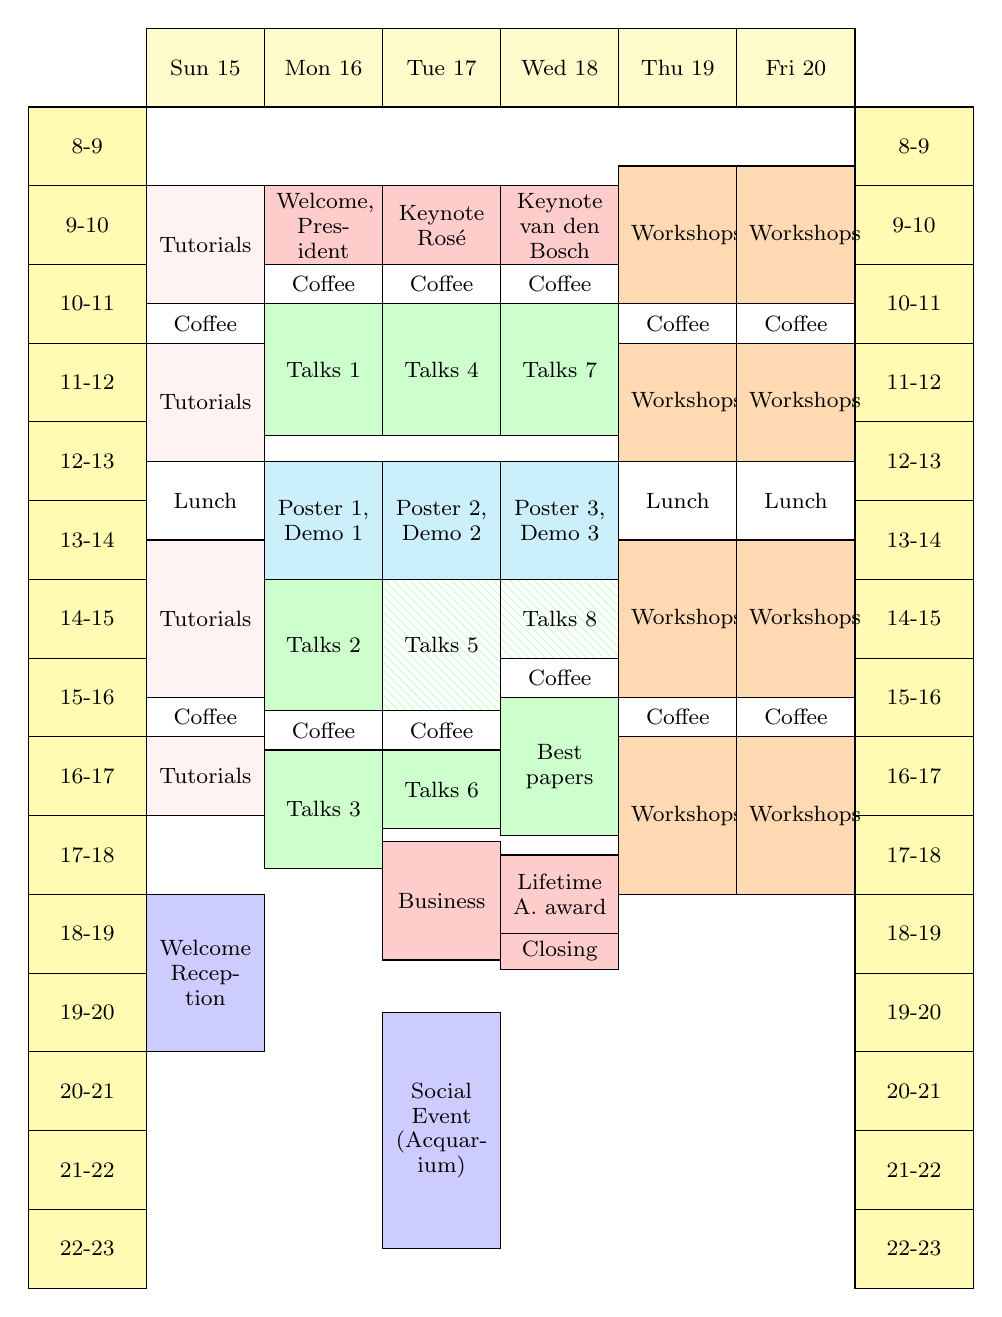
\begin{tikzpicture}[x=\daywidth, y=-1cm, node distance=0 cm,outer sep = 0pt]
% Style for Days
\tikzstyle{day}=[draw, rectangle,  minimum height=1cm, minimum width=\daywidth, fill=yellow!20,anchor=south west]
% Style for hours
\tikzstyle{hour}=[draw, rectangle, minimum height=1 cm, minimum width=1.5 cm, fill=yellow!30,anchor=north east]
\tikzstyle{hourr}=[draw, rectangle, minimum height=1 cm, minimum width=1.5 cm, fill=yellow!30,anchor=north west]
% Styles for events
% Duration of sequences
\tikzstyle{hours}=[rectangle,draw, minimum width=\daywidth, anchor=north west,text centered,text width=4 em]
\tikzstyle{1hour}=[hours,minimum height=1cm]
\tikzstyle{2hours}=[hours,minimum height=2cm]
\tikzstyle{3hours}=[hours,minimum height=3cm]
%Style for type of sequence 
\tikzstyle{Ang2h}=[2hours,fill=green!20]
\tikzstyle{Phys2h}=[2hours,fill=red!20]
\tikzstyle{Math2h}=[2hours,fill=blue!20]
\tikzstyle{TIPE2h}=[2hours,fill=blue!10]
\tikzstyle{TP2h}=[2hours, pattern=north east lines, pattern color=magenta]
\tikzstyle{G3h}=[3hours, pattern=north west lines, pattern color=magenta!60!white]
\tikzstyle{Planche}=[1hour,fill=white]
% Positioning labels for days and hours
\node[day] (sun) at (1,8) {Sun 15};
\node[day] (mon) [right = of sun] {Mon 16};
\node[day] (tue) [right = of mon] {Tue 17};
\node[day] (wed) [right = of tue] {Wed 18};
\node[day] (thu) [right = of wed] {Thu 19};
\node[day] (fri) [right = of thu] {Fri 20};
\node[hour] (8-9) at (1,8) {8-9};
\node[hour] (9-10) [below = of 8-9] {9-10};
\node[hour] (10-11) [below= of 9-10] {10-11};
\node[hour] (11-12) [below = of 10-11] {11-12};
\node[hour] (12-13) [below  = of 11-12] {12-13};
\node[hour] (13-14) [below = of 12-13] {13-14};
\node[hour] (14-15) [below = of 13-14] {14-15};
\node[hour] (15-16) [below = of 14-15] {15-16};
\node[hour] (16-17) [below = of 15-16] {16-17};
\node[hour] (17-18) [below = of 16-17] {17-18};
\node[hour] (18-19) [below = of 17-18] {18-19};
\node[hour] (19-20) [below = of 18-19] {19-20};
\node[hour] (20-21) [below = of 19-20] {20-21};
\node[hour] (21-22) [below = of 20-21] {21-22};
\node[hour] (22-23) [below = of 21-22] {22-23};
%
\node[hourr] (8-9) at (7,8) {8-9};
\node[hourr] (9-10) [below = of 8-9] {9-10};
\node[hourr] (10-11) [below= of 9-10] {10-11};
\node[hourr] (11-12) [below = of 10-11] {11-12};
\node[hourr] (12-13) [below  = of 11-12] {12-13};
\node[hourr] (13-14) [below = of 12-13] {13-14};
\node[hourr] (14-15) [below = of 13-14] {14-15};
\node[hourr] (15-16) [below = of 14-15] {15-16};
\node[hourr] (16-17) [below = of 15-16] {16-17};
\node[hourr] (17-18) [below = of 16-17] {17-18};
\node[hourr] (18-19) [below = of 17-18] {18-19};
\node[hourr] (19-20) [below = of 18-19] {19-20};
\node[hourr] (20-21) [below = of 19-20] {20-21};
\node[hourr] (21-22) [below = of 20-21] {21-22};
\node[hourr] (22-23) [below = of 21-22] {22-23};
%Position of sequences
\node[hours,minimum height=1.5cm,fill=pink!20] at (1,9) {Tutorials};
\node[Planche,minimum height=0.5cm] at (1,10.5) {Coffee};
\node[hours,minimum height=1.5cm,fill=pink!20] at (1,11) {Tutorials};
\node[Planche] at (1,12.5) {Lunch};
\node[hours,minimum height=2cm,fill=pink!20] at (1,13.5) {Tutorials};
\node[Planche,minimum height=0.5cm] at (1,15.5) {Coffee};
\node[hours,minimum height=1cm,fill=pink!20] at (1,16) {Tutorials};
\node[hours,minimum height=2cm,fill=blue!20] at (1,18) {Welcome Reception};
%
\node[hours,minimum height=1cm,fill=red!20] at (2,9) {Welcome, President};
\node[Planche,minimum height=0.5cm] at (2,10) {Coffee};
\node[hours,minimum height=1.667cm,fill=green!20] at (2,10.5) {Talks 1};
\node[hours,minimum height=1.5cm,fill=cyan!20] at (2,12.5) {Poster 1, Demo 1};
\node[hours,minimum height=1.667cm,fill=green!20] at (2,14) {Talks 2};
\node[Planche,minimum height=0.5cm] at (2,15.667) {Coffee};
\node[hours,minimum height=1.5cm,fill=green!20] at (2,16.1667) {Talks 3};
%
\node[hours,minimum height=1cm,fill=red!20] at (3,9) {Keynote Ros\'{e}};
\node[Planche,minimum height=0.5cm] at (3,10) {Coffee};
\node[hours,minimum height=1.667cm,fill=green!20] at (3,10.5) {Talks 4};
\node[hours,minimum height=1.5cm,fill=cyan!20] at (3,12.5) {Poster 2, Demo 2};
\node[hours,minimum height=1.667cm,pattern color=green!20,pattern=north west lines] at (3,14) {Talks 5};
\node[Planche,minimum height=0.5cm] at (3,15.667) {Coffee};
\node[hours,minimum height=1cm,fill=green!20] at (3,16.1667) {Talks 6};
\node[hours,minimum height=1.5cm,fill=red!20] at (3,17.3333) {Business};
\node[hours,minimum height=3cm,fill=blue!20] at (3,19.5) {Social Event (Acquarium)};
%
\node[hours,minimum height=1cm,fill=red!20] at (4,9) {Keynote van den Bosch};
\node[Planche,minimum height=0.5cm] at (4,10) {Coffee};
\node[hours,minimum height=1.667cm,fill=green!20] at (4,10.5) {Talks 7};
\node[hours,minimum height=1.5cm,fill=cyan!20] at (4,12.5) {Poster 3, Demo 3};
\node[hours,minimum height=1cm,pattern color=green!20,pattern=north west lines] at (4,14) {Talks 8};
\node[Planche,minimum height=0.5cm] at (4,15) {Coffee};
\node[hours,minimum height=1.75cm,fill=green!20] at (4,15.5) {Best papers};
\node[hours,minimum height=1cm,fill=red!20] at (4,17.5) {Lifetime A. award};
\node[hours,minimum height=0.25cm,fill=red!20] at (4,18.5) {Closing};
%
\node[hours,minimum height=1.75cm,fill=orange!30] at (5,8.75) {Workshops};
\node[Planche,minimum height=0.5cm] at (5,10.50) {Coffee};
\node[hours,minimum height=1.5cm,fill=orange!30] at (5,11) {Workshops};
\node[Planche,minimum height=1cm] at (5,12.50) {Lunch};
\node[hours,minimum height=2cm,fill=orange!30] at (5,13.5) {Workshops};
\node[Planche,minimum height=0.5cm] at (5,15.50) {Coffee};
\node[hours,minimum height=2cm,fill=orange!30] at (5,16) {Workshops};
%
\node[hours,minimum height=1.75cm,fill=orange!30] at (6,8.75) {Workshops};
\node[Planche,minimum height=0.5cm] at (6,10.50) {Coffee};
\node[hours,minimum height=1.5cm,fill=orange!30] at (6,11) {Workshops};
\node[Planche,minimum height=1cm] at (6,12.50) {Lunch};
\node[hours,minimum height=2cm,fill=orange!30] at (6,13.5) {Workshops};
\node[Planche,minimum height=0.5cm] at (6,15.50) {Coffee};
\node[hours,minimum height=2cm,fill=orange!30] at (6,16) {Workshops};
\end{tikzpicture}

\noindent\emph{Cover design by Carrie Chilton}\\\index{Chilton, Carrie}
\noindent\emph{Handbook assembled by Jey Han Lau and Trevor Cohn}\\\index{Lau, Jey Han} 
\index{Cohn, Trevor}
\emph{Printing by Minuteman Press}

\newpage
\cleardoublepage
\fancyfoot[C]{\thepage}
\frontmatter

%% SPONSORS %%%%%%%%%%%%%%%%%%%%%%%%%%%%%%%%%%%%%%%%%%%%%%%%%%%%%

%% Putting on back cover

%% \addcontentsline{toc}{chapter}{Sponsorship}
%% \thispagestyle{empty}
%% \setheaders{}{}
%% 
Diamond Sponsors:\\

\begin{tabular}{ c c c }
\raisebox{-0.5\height}{\includegraphics[width=2cm]{content/sponsors/logos/google.png}} & \raisebox{-0.5\height}{\includegraphics[width=2cm]{content/sponsors/logos/bytedance-toutiao.png}} & \raisebox{-0.5\height}{\includegraphics[width=2cm]{content/sponsors/logos/samsung.jpg}} \\ 
\raisebox{-0.5\height}{\includegraphics[width=2cm]{content/sponsors/logos/Apple_Logo_429C_RGB_090318_clearspace.pdf}} & 
\raisebox{-0.5\height}{\includegraphics[width=2cm]{content/sponsors/logos/facebook.png}} & 
\end{tabular}
\\

%\includegraphics[width=3.5cm]{content/sponsors/logos/google.png}\qquad
%\includegraphics[width=3.5cm]{content/sponsors/logos/bytedance-toutiao.png}\qquad
%\includegraphics[width=3.5cm]{content/sponsors/logos/samsung.jpg}\\%\qquad
%\includegraphics[width=3.5cm]{content/sponsors/logos/Apple_Logo_429C_RGB_090318_clearspace.pdf}\qquad
%\includegraphics[width=3.5cm]{content/sponsors/logos/facebook.png}\\

Platinum Sponsors:\\

\begin{tabular}{ c c c }
	\raisebox{-0.5\height}{\includegraphics[width=3.2cm]{content/sponsors/logos/amazon.png}} & \raisebox{-0.5\height}{\includegraphics[width=3.5cm]{content/sponsors/logos/baidu.png}} & \raisebox{-0.5\height}{\includegraphics[width=3.5cm]{content/sponsors/logos/jingdong.png}} \\ 
	&&\\
	\raisebox{-0.5\height}{\includegraphics[width=3.5cm]{content/sponsors/logos/rit.png}} & 
	\raisebox{-0.5\height}{\includegraphics[width=3.5cm]{content/sponsors/logos/tencent.png}} & \\
\end{tabular}
\\
\\
\\

%\includegraphics[width=3.1cm]{content/sponsors/logos/amazon.png}\qquad
%\includegraphics[width=3.4cm]{content/sponsors/logos/baidu.png}\qquad
%\includegraphics[width=3.4cm]{content/sponsors/logos/jingdong.png}\qquad
%\includegraphics[width=3.4cm]{content/sponsors/logos/rit.png}\qquad
%\includegraphics[width=3.5cm]{content/sponsors/logos/tencent.png}\\

Gold Sponsors:\\

\begin{tabular}{ c c c }
	\raisebox{-0.5\height}{\LARGE \bf IBM Research} & \raisebox{-0.5\height}{\includegraphics[width=4cm]{content/sponsors/logos/microsoft.png}} & \raisebox{-0.5\height}{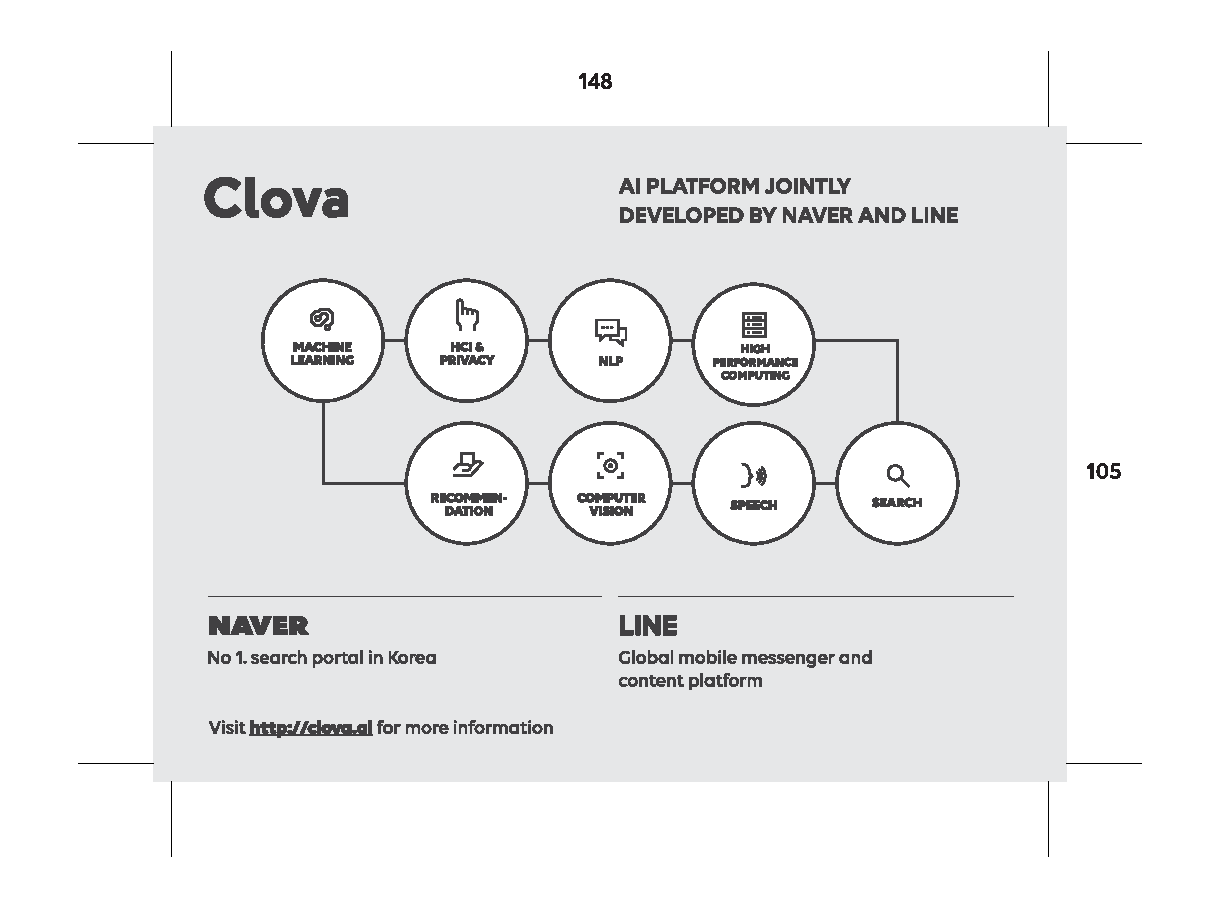
\includegraphics[width=3.9cm]{content/sponsors/logos/naver.png}} \\
	&&\\
	\raisebox{-0.5\height}{\includegraphics[width=3.9cm]{content/sponsors/logos/cvte.jpg}} & 
	\raisebox{-0.5\height}{\includegraphics[width=4.5cm]{content/sponsors/logos/dhcrc.jpg}} & 
\end{tabular}
\\
\\
\\

%IBM Research\qquad 
%\includegraphics[width=3.6cm]{content/sponsors/logos/microsoft.png}\qquad
%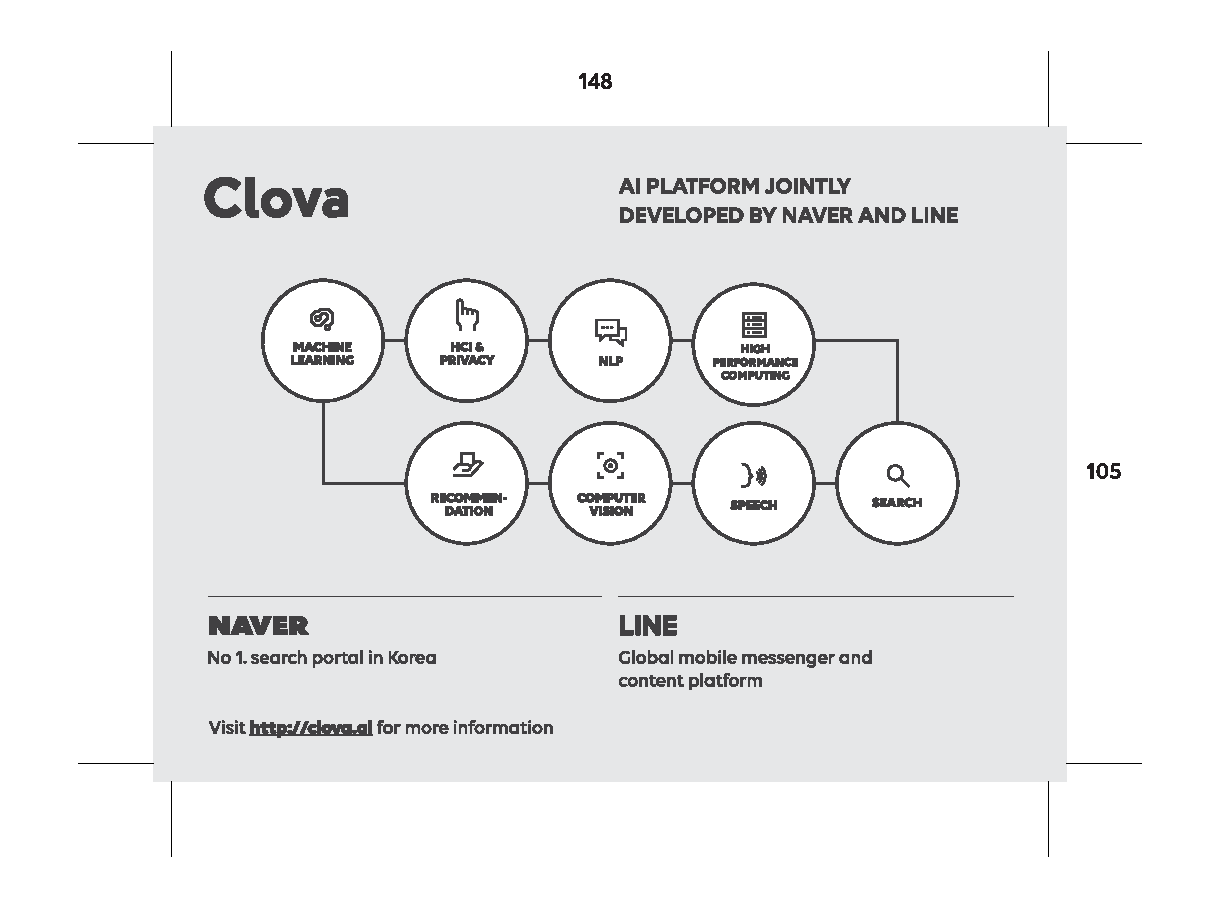
\includegraphics[width=3.6cm]{content/sponsors/logos/naver.png}\qquad
%\includegraphics[width=3.6cm]{content/sponsors/logos/cvte.jpg}\\

Silver Sponsors:\\

\begin{tabular}{ c c c c }
	\raisebox{-0.5\height}{\includegraphics[width=3.5cm]{content/sponsors/logos/nuance.png}}\quad & 
	\raisebox{-0.5\height}{\includegraphics[width=2.1cm]{content/sponsors/logos/huawei.png}}\quad\quad & 
	\raisebox{-0.5\height}{\includegraphics[width=2.1cm]{content/sponsors/logos/elsevier.png}}\quad &
	\raisebox{-0.5\height}{\includegraphics[width=3.5cm]{content/sponsors/logos/duolingo-cropped.jpg}} \\
\end{tabular}


%\includegraphics[width=3.6cm]{content/sponsors/logos/nuance.png}\qquad\qquad
%\includegraphics[width=2cm]{content/sponsors/logos/huawei.png}\qquad\qquad
%\includegraphics[width=2cm]{content/sponsors/logos/elsevier.png}\qquad\qquad
%\includegraphics[width=3.7cm]{content/sponsors/logos/duolingo.jpg}
%\qquad
%%\includegraphics[width=3.5cm]{content/sponsors/logos/tencent.png}\\

\newpage

Bronze Sponsors:\\

%\includegraphics[width=3.6cm]{content/sponsors/logos/isi-nlp.jpg}\qquad 

\begin{tabular}{ c c }
	\raisebox{-0.5\height}{\includegraphics[width=3.5cm]{content/sponsors/logos/isi-nlp.jpg}}\quad\quad & \raisebox{-0.5\height}{\includegraphics[width=6.5cm]{content/sponsors/logos/dstg.pdf}}\quad\quad \\
\end{tabular}
\\
\\

%\includegraphics[width=3.6cm]{content/sponsors/logos/isi-nlp.jpg}\qquad 
%\includegraphics[width=3.6cm]{content/sponsors/logos/DSTGroup-Logo-Vert.jpg}

Supporters: \\

\begin{tabular}{ c c }
	\raisebox{-0.5\height}{\includegraphics[width=3.5cm]{content/sponsors/logos/roam.png}}\quad\quad & \raisebox{-0.5\height}{\includegraphics[width=3.5cm]{content/sponsors/logos/sap.png}}\quad\quad \\
\end{tabular}
\\
\\

%\includegraphics[width=3.5cm]{content/sponsors/logos/roam.png} \qquad
%\includegraphics[width=3.5cm]{content/sponsors/logos/sap.png}\\

Student Volunteers Sponsors: \\

\quad\enskip\includegraphics[width=3.5cm]{content/sponsors/logos/data61.png}


%% TOC %%%%%%%%%%%%%%%%%%%%%%%%%%%%%%%%%%%%%%%%%%%%%%%%%%%%%%%%%%

\addcontentsline{toc}{chapter}{Table of Contents}
\setcounter{tocdepth}{2}
\tableofcontents
\mainmatter
\pagestyle{fancy}

%% PREFACE %%%%%%%%%%%%%%%%%%%%%%%%%%%%%%%%%%%%%%%%%%%%%%%%%%%%%%

\chapter{Conference Information}

\section{Message from the General Chair}\vspace{2em}
\setheaders%
    {Message from the General Chair}%
    {Message from the General Chair}
\thispagestyle{emptyheader}

\setlength{\parskip}{.7ex}

TOUPDATE \\

\vspace{1.0em} 
\noindent ACL 2020 General Chair\\
% Claire Cardie, Cornell University\\
% \index{Cardie, Claire}

\clearpage
\section{Message from the Program Committee Co-Chairs}\vspace{2em}
\setheaders%
    {Message from the Program Committee Co-Chairs}%
    {Message from the Program Committee Co-Chairs}
\thispagestyle{emptyheader}
%\renewcommand{\large}{\fontsize{9}{11}\selectfont}
% that's a hack to make this part nicely fill the pages

\setlength{\parskip}{.7ex}
%\setlength{\parindent}{0pt}


Welcome to the 56th Annual Meeting of the Association for Computational Linguistics 2018 -- or ACL 2018 for short. 

In September 2017, Program Committee Co-Chairs (PCs) posted the call for nominations of Area Chairs (AC), Reviewers and Invited Speakers. We received 752 responses in total. Overall, out of 388 valid nominations for area chairs, 299 unique persons were suggested; 110 persons were self-nominations. About 70\% of the 56 selected area chairs (later expanded to 61 area chairs due to the high number of submissions) were nominated by the community. For the reviewers, we collected 936 valid nominations. At the PhD level, 139 persons were self-nominations and 129 were nominated by others. At the Postdoc/Ass.Prof.~level, 160 were self-nominated, 112 nominated by others. At the Prof.~level, 221 persons were self-nominated, 175 nominated by others. 

We received 138 unique nominations for invited speakers, from which two invited speakers of the conference were selected: 
\begin{itemize}
	\item Carolyn Penstein Rosé, Language Technologies Institute at Carnegie Mellon University, USA
	\item Anton van den Hengel, Australian Centre for Visual Technologies at University of Adelaide, Australia
\end{itemize}

%% # reviewers: 1473 (primary), 137 (secondary) -> total 1610
%% # good reviewers: 192

Our community is steadily growing: in total, 1621 submissions were received right after the submission deadline: 1045 long, 576 short papers. 13 erroneous submissions were deleted or withdrawn in the preliminary checks by PCs. 25 papers were rejected without review (16 long, 9 short); the reasons are the violation of the ACL 2018 style and dual submission guidelines. 32 papers were withdrawn before the review period started; the main reason was that the papers have been accepted as the short papers at NAACL HLT 2018. In total, 1551 papers went into the reviewing phase: 1021 long, 530 short papers. 1610 reviewers (1473 primary and 137 secondary reviewers) were involved in the reviewing process; each reviewer has reviewed about 3 papers on average.  3 long and 4 short papers were withdrawn during the reviewing period, and finally 1018 long and 526 short papers were considered during the acceptance decision phase.

The assignment of papers to areas and reviewers has been done in multiple rounds. First round: Initial assignments of papers to areas were determined automatically with the help of the authors’ input, while PCs went through all submissions and moved papers to other areas, considering COI and the topical fit. PCs assigned one AC as a meta-reviewer to each paper using Toronto Paper Matching System (TPMS) scores. Second round: ACs looked into the papers in their area, and adjusted meta-reviewer assignments. ACs sent a report to PCs if they found any problems. Third round: PCs made the final decision, considering the workload balance, possible COIs and the topical fit. Fourth round: ACs decided which reviewers would review each paper, based on AC’s knowledge about the reviewers, TPMS scores, reviewers’ bids, and COI.

We have introduced several innovations to the reviewing process. One of them is an argument-based review form. The reviewers were asked to provide arguments for and against the paper. This has been tremendously helpful for ACs and PCs to analyze the reviews and come up with final recommendations. The authors were asked to respond to the con arguments during the rebuttal. In coordination with the NAACL HLT 2018 PCs, we plan to do some analytics on anonymized reviews and rebuttal statements, with the consent of the reviewers and authors. Our purpose is to improve the quality of the review process. The data will be compiled into a unique corpus for NLP, and will be made available to the research community after appropriate anonymization checks, at the earliest in 2 years after ACL 2018. We hope to provide data on \emph{how to review} to younger researchers, and to improve the transparency of the reviewing process in general. 

The ACL 2018 conference is super-competitive: We accepted 256 out of 1018 submitted long papers and 125 out of 526 short papers, with an overall acceptance rate of 24.7\%. The details of the review process are available at the conference homepage. 
Criteria of acceptance were mainly: 
\begin{itemize}
	\item strengths/weaknesses raised by reviewers and their significance;
	\item the result of discussions and author responses;
	\item contribution to CL as the science of language: whether the paper advances (or contributes to) our understanding of language in any way;
	\item diversity: we do not want to fill ACL with similar papers like achieving 1\% improvement on a well-known task.  
\end{itemize}
We also considered the balance of paper types, topics and contributions and
re-considered the acceptance when reviewers reported any problem in preliminary checks (\textit{Appropriateness} to \textit{Handling of Human Participants}).

Continuing the tradition, ACL 2018 will feature 20 papers
which were accepted for publication in the Transactions of the
Association for Computational Linguistics (TACL). The TACL papers
were split into 10 oral presentations and 10 poster presentations.

There are many people to thank for who have worked diligently to
make ACL 2018 possible. All names are listed in the Program Committee section of the Front
Matter. 

Since the conference size continues to grow and the organizational complexity increases, we have introduced the role of Program Committee Co-Chair Assistants. In total, 5 senior researchers have supported the PCs during most intensive work phases to handle the communication in a timely manner, draft various documents and effectively prepare decisions.

Thanks to our area chairs for their hard work on recruiting reviewers, managing reviews,
leading discussions, and making recommendations.  

This program certainly would not be possible without the help of
the 1610 reviewers.
%Their names are listed in the Program Committee section.  
In particular, 192 reviewers from this list were recognized
by the area chairs as outstanding reviewers who have turned in exceptionally
well-written and constructive reviews and who have actively engaged themselves in
the post-rebuttal discussions. 

We are also deeply indebted to the best paper selection committee which consists
of 22 members. They had to additionally review 6-8 papers according to the best paper criteria on short notice. Their time and effort in recommending the best paper awards is much appreciated.

We also would like to thank many colleagues for generously sharing their experience in
organizing prior ACL conferences and for their advice. We are
grateful for the guidance and the support of the ACL presidents
Joakim Nivre and Marti Hearst, and the ACL board. We also would like to thank
the publication co-chairs Shay Cohen, Kevin Gimpel and Wei Lu (Advisory) and the handbook chair Jey Han Lau for putting
together the proceedings and the conference handbook; and Rich Gerber from Softconf for always being responsive to our
requests. We would like to thank the ACL Business Manager Priscilla Rasmussen for helping us to sort important things out. 
Finally, this conference could not have happened without the efforts
of the general chair, Claire Cardie. We thank her for the leadership and advice, especially when matters got complicated.

We hope you will enjoy ACL 2018 and contribute to the future success of our community!

%\noindent\includegraphics[scale=1.5]{content/fmatter/easteregg.pdf}

\vspace{1.0em}
\noindent ACL 2018 Program Committee Co-Chairs \\
Iryna Gurevych, TU Darmstadt, Germany \\
Yusuke Miyao, National Institute of Informatics, Japan
\index{Gurevych, Iryna}
\index{Miyao, Yusuke}


\clearpage%{\thispagestyle{emptyheader}\cleardoublepage}
\setheaders{}{}
\markboth{}{} % clear the right header
\markright{}{} % clear the right header

\section{Organizing Committee}{}

\setlength{\parindent}{0pt}

TOUPDATE % BUG

{\bf General Chair} \\
Claire Cardie, Cornell University

{\bf Program Chairs} \\
Iryna Gurevych, TU Darmstadt\\
Yusuke Miyao, National Institute of Informatics

{\bf Workshop Chairs} \\
Brendan O’Connor, University of Massachusetts Amherst\\
Eva Maria Vecchi, University of Cambridge

{\bf Tutorial Chairs} \\
Yoav Artzi, Cornell University\\
Jacob Eisenstein, Georgia Institute of Technology

{\bf Demo Chairs} \\
Fei Liu, University of Central Florida\\
Thamar Solorio, University of Houston

{\bf Publication Chairs} \\
Shay Cohen, University of Edinburgh\\
Kevin Gimpel, Toyota Technological Institute at Chicago\\
Wei Lu, Singapore University of Technology and Design (Advisory)

{\bf Exhibits Coordinator} \\
Karin Verspoor, University of Melbourne

{\bf Conference Handbook Chairs} \\
Jey Han Lau, IBM Research\\
Trevor Cohn, University of Melbourne

{\bf Publicity Chair} \\
Sarvnaz Karimi, CSIRO

{\bf Local Sponsorship Chair} \\
Cecile Paris, CSIRO

{\bf Student Volunteer Coordinator} \\
Karin Verspoor, University of Melbourne

{\bf Local Chairs} \\
Tim Baldwin, University of Melbourne\\
Karin Verspoor, University of Melbourne\\
Trevor Cohn, University of Melbourne

{\bf Student Research Workshop Organisers} \\
Vered Shwartz, Bar-Ilan University\\
Jeniya Tabassum, Ohio State University\\
Rob Voigt, Stanford University

{\bf Faculty Advisors to the Student Research Workshop} \\
Marie-Catherine de Marneffe, Ohio State University\\
Wanxiang Che, Harbin Institute of Technology\\
Malvina Nissim, University of Groningen

{\bf Webmaster} \\
Andrew MacKinlay, Culture Amp / University of Melbourne

%%%%%%%%%%%%%%%%%%%%%%%%%%%%%%%%%%%%%%%%%%%%%%%%%%%%%%%%%%%%%%%%%%%%%%%%

\clearpage
\section{Program Committee}
\setlength{\parindent}{0pt}

TOUPDATE % BUG

{\bf Program Committee Co-chairs} \\
Iryna Gurevych, TU Darmstadt, Germany \\
Yusuke Miyao, National Institute of Informatics, Japan

{\bf Program Committee Co-Chair Assistants} \\
Yang Gao, TU Darmstadt, Germany \\
Ivan Habernal, TU Darmstadt, Germany \\
Sang Phan, National Institute of Informatics, Japan \\
Steffen Eger, TU Darmstadt, Germany \\
Christian Meyer, TU Darmstadt, Germany

{\bf Area Chairs} \\
(Senior Area Chairs are indicated in boldface.)

\emph{Dialogue and Interactive Systems} \\
\hspace*{5mm}\textbf{Asli Celikyilmaz} \\
\hspace*{5mm}Verena Rieser \\
\hspace*{5mm}Milica Gasic \\
\hspace*{5mm}Jason Williams

\emph{Discourse and Pragmatics} \\
\hspace*{5mm}Manfred Stede \\
\hspace*{5mm}\textbf{Ani Nenkova}

\emph{Document Analysis} \\
\hspace*{5mm}\textbf{Hang Li} \\
\hspace*{5mm}Yiqun Liu \\
\hspace*{5mm}Eugene Agichtein

\emph{Generation} \\
\hspace*{5mm}Ioannis Konstas \\
\hspace*{5mm}\textbf{Claire Gardent}

\emph{Information Extraction and Text Mining} \\
\hspace*{5mm}Feiyu Xu \\
\hspace*{5mm}Kevin Cohen \\
\hspace*{5mm}Zhiyuan Liu \\
\hspace*{5mm}\textbf{Ralph Grishman} \\
\hspace*{5mm}Yi Yang \\
\hspace*{5mm}Nazli Goharian

\emph{Linguistic Theories, Cognitive Modeling and Psycholinguistics}\\
\hspace*{5mm}\textbf{Shuly Wintner} \\
\hspace*{5mm}\textbf{Tim O'Donnell}

\emph{Machine Learning} \\
\hspace*{5mm}Andre Martins \\
\hspace*{5mm}Ariadna Quattoni \\
\hspace*{5mm}\textbf{Jun Suzuki}

\emph{Machine Translation} \\
\hspace*{5mm}Yang Liu (Tsinghua University)\\
\hspace*{5mm}\textbf{Matt Post} \\
\hspace*{5mm}Lucia Specia \\
\hspace*{5mm}Dekai Wu

\emph{Multidisciplinary and Area Chair COI}\\
\hspace*{5mm}\textbf{Yoav Goldberg} \\
\hspace*{5mm}\textbf{Anders Søgaard} \\
\hspace*{5mm}\textbf{Mirella Lapata}

\emph{Multilinguality}\\
\hspace*{5mm}\textbf{Bernardo Magnini} \\
\hspace*{5mm}Tristan Miller

\emph{Phonology, Morphology, and Word Segmentation} \\
\hspace*{5mm}Graham Neubig \\
\hspace*{5mm}\textbf{Hai Zhao}

\emph{Question Answering}\\
\hspace*{5mm}\textbf{Lluís Màrquez} \\
\hspace*{5mm}Teruko Mitamura \\
\hspace*{5mm}Zornitsa Kozareva \\
\hspace*{5mm}Richard Socher

\emph{Resources and Evaluation}\\
\hspace*{5mm}Gerard de Melo \\
\hspace*{5mm}Sara Tonelli \\
\hspace*{5mm}\textbf{Karën Fort}

\emph{Sentence-level Semantics} \\
\hspace*{5mm}\textbf{Luke Zettlemoyer} \\
\hspace*{5mm}Ellie Pavlick \\
\hspace*{5mm}Jacob Uszkoreit

\emph{Sentiment Analysis and Argument Mining} \\
\hspace*{5mm}Smaranda Muresan \\
\hspace*{5mm}Benno Stein \\
\hspace*{5mm}\textbf{Yulan He}

\emph{Social Media}\\
\hspace*{5mm}David Jurgens \\
\hspace*{5mm}\textbf{Jing Jiang}

\emph{Summarization}\\
\hspace*{5mm}\textbf{Kathleen McKeown} \\
\hspace*{5mm}Xiaodan Zhu

\emph{Tagging, Chunking, Syntax, and Parsing} \\
\hspace*{5mm}\textbf{Liang Huang} \\
\hspace*{5mm}Weiwei Sun \\
\hspace*{5mm}Željko Agić \\
\hspace*{5mm}Yue Zhang

\emph{Textual Inference and Other Areas of Semantics}\\
\hspace*{5mm}\textbf{Michael Roth} \\
\hspace*{5mm}\textbf{Fabio Massimo Zanzotto}

\emph{Vision, Robotics, Multimodal, Grounding and Speech}\\
\hspace*{5mm}\textbf{Yoav Artzi} \\
\hspace*{5mm}Shinji Watanabe \\
\hspace*{5mm}Timothy Hospedales

\emph{Word-level Semantics}\\
\hspace*{5mm}Ekaterina Shutova \\
\hspace*{5mm}\textbf{Roberto Navigli}

{\bf Best Paper Selection Committee} \\
Timothy	Baldwin \\
Pushpak	Bhattacharyya \\
Phil	Blunsom \\
Johan	Bos \\
Jordan	Boyd-Graber \\
Trevor	Cohn \\
Vera	Demberg \\
Kevin	Duh \\
Katrin	Erk \\
Mark	Johnson \\
Yang	Liu (Tsinghua University)\\
Yuji	Matsumoto \\
Jong	Park \\
Ellie	Pavlick \\
Simone Paolo	Ponzetto \\
Sebastian	Riedel \\
Carolyn	Penstein Rosé \\
Noah A.~Smith \\
Anders	Søgaard \\
Ivan	Titov \\
Benjamin	Van Durme \\
Ming	Zhou



%% \clearpage
%
Diamond Sponsors:\\

\begin{tabular}{ c c c }
\raisebox{-0.5\height}{\includegraphics[width=2cm]{content/sponsors/logos/google.png}} & \raisebox{-0.5\height}{\includegraphics[width=2cm]{content/sponsors/logos/bytedance-toutiao.png}} & \raisebox{-0.5\height}{\includegraphics[width=2cm]{content/sponsors/logos/samsung.jpg}} \\ 
\raisebox{-0.5\height}{\includegraphics[width=2cm]{content/sponsors/logos/Apple_Logo_429C_RGB_090318_clearspace.pdf}} & 
\raisebox{-0.5\height}{\includegraphics[width=2cm]{content/sponsors/logos/facebook.png}} & 
\end{tabular}
\\

%\includegraphics[width=3.5cm]{content/sponsors/logos/google.png}\qquad
%\includegraphics[width=3.5cm]{content/sponsors/logos/bytedance-toutiao.png}\qquad
%\includegraphics[width=3.5cm]{content/sponsors/logos/samsung.jpg}\\%\qquad
%\includegraphics[width=3.5cm]{content/sponsors/logos/Apple_Logo_429C_RGB_090318_clearspace.pdf}\qquad
%\includegraphics[width=3.5cm]{content/sponsors/logos/facebook.png}\\

Platinum Sponsors:\\

\begin{tabular}{ c c c }
	\raisebox{-0.5\height}{\includegraphics[width=3.2cm]{content/sponsors/logos/amazon.png}} & \raisebox{-0.5\height}{\includegraphics[width=3.5cm]{content/sponsors/logos/baidu.png}} & \raisebox{-0.5\height}{\includegraphics[width=3.5cm]{content/sponsors/logos/jingdong.png}} \\ 
	&&\\
	\raisebox{-0.5\height}{\includegraphics[width=3.5cm]{content/sponsors/logos/rit.png}} & 
	\raisebox{-0.5\height}{\includegraphics[width=3.5cm]{content/sponsors/logos/tencent.png}} & \\
\end{tabular}
\\
\\
\\

%\includegraphics[width=3.1cm]{content/sponsors/logos/amazon.png}\qquad
%\includegraphics[width=3.4cm]{content/sponsors/logos/baidu.png}\qquad
%\includegraphics[width=3.4cm]{content/sponsors/logos/jingdong.png}\qquad
%\includegraphics[width=3.4cm]{content/sponsors/logos/rit.png}\qquad
%\includegraphics[width=3.5cm]{content/sponsors/logos/tencent.png}\\

Gold Sponsors:\\

\begin{tabular}{ c c c }
	\raisebox{-0.5\height}{\LARGE \bf IBM Research} & \raisebox{-0.5\height}{\includegraphics[width=4cm]{content/sponsors/logos/microsoft.png}} & \raisebox{-0.5\height}{\includegraphics[width=3.9cm]{content/sponsors/logos/naver.png}} \\
	&&\\
	\raisebox{-0.5\height}{\includegraphics[width=3.9cm]{content/sponsors/logos/cvte.jpg}} & 
	\raisebox{-0.5\height}{\includegraphics[width=4.5cm]{content/sponsors/logos/dhcrc.jpg}} & 
\end{tabular}
\\
\\
\\

%IBM Research\qquad 
%\includegraphics[width=3.6cm]{content/sponsors/logos/microsoft.png}\qquad
%\includegraphics[width=3.6cm]{content/sponsors/logos/naver.png}\qquad
%\includegraphics[width=3.6cm]{content/sponsors/logos/cvte.jpg}\\

Silver Sponsors:\\

\begin{tabular}{ c c c c }
	\raisebox{-0.5\height}{\includegraphics[width=3.5cm]{content/sponsors/logos/nuance.png}}\quad & 
	\raisebox{-0.5\height}{\includegraphics[width=2.1cm]{content/sponsors/logos/huawei.png}}\quad\quad & 
	\raisebox{-0.5\height}{\includegraphics[width=2.1cm]{content/sponsors/logos/elsevier.png}}\quad &
	\raisebox{-0.5\height}{\includegraphics[width=3.5cm]{content/sponsors/logos/duolingo-cropped.jpg}} \\
\end{tabular}


%\includegraphics[width=3.6cm]{content/sponsors/logos/nuance.png}\qquad\qquad
%\includegraphics[width=2cm]{content/sponsors/logos/huawei.png}\qquad\qquad
%\includegraphics[width=2cm]{content/sponsors/logos/elsevier.png}\qquad\qquad
%\includegraphics[width=3.7cm]{content/sponsors/logos/duolingo.jpg}
%\qquad
%%\includegraphics[width=3.5cm]{content/sponsors/logos/tencent.png}\\

\newpage

Bronze Sponsors:\\

%\includegraphics[width=3.6cm]{content/sponsors/logos/isi-nlp.jpg}\qquad 

\begin{tabular}{ c c }
	\raisebox{-0.5\height}{\includegraphics[width=3.5cm]{content/sponsors/logos/isi-nlp.jpg}}\quad\quad & \raisebox{-0.5\height}{\includegraphics[width=6.5cm]{content/sponsors/logos/dstg.pdf}}\quad\quad \\
\end{tabular}
\\
\\

%\includegraphics[width=3.6cm]{content/sponsors/logos/isi-nlp.jpg}\qquad 
%\includegraphics[width=3.6cm]{content/sponsors/logos/DSTGroup-Logo-Vert.jpg}

Supporters: \\

\begin{tabular}{ c c }
	\raisebox{-0.5\height}{\includegraphics[width=3.5cm]{content/sponsors/logos/roam.png}}\quad\quad & \raisebox{-0.5\height}{\includegraphics[width=3.5cm]{content/sponsors/logos/sap.png}}\quad\quad \\
\end{tabular}
\\
\\

%\includegraphics[width=3.5cm]{content/sponsors/logos/roam.png} \qquad
%\includegraphics[width=3.5cm]{content/sponsors/logos/sap.png}\\

Student Volunteers Sponsors: \\

\quad\enskip\includegraphics[width=3.5cm]{content/sponsors/logos/data61.png}

\clearpage%{\thispagestyle{emptyheader}\cleardoublepage}
\setheaders{}{}

\setheaders{}{}
\section{Meal Info}{}

The following meals are provided as part of your registration fee:

\begin{itemize}
\item Mid-morning breaks include coffee, tea, water and snacks
	in the Melbourne Room and level 2 foyer
\item A light lunch of sandwiches and a muffin is provided during each
	of the midday poster sesions on Monday -- Wednesday,
	in the Melbourne Room
\item Mid-Afternoon breaks include coffee, tea, water, and 
	snacks in the Melbourne Room and level 2 foyer
\end{itemize}

Light refreshments are provided for students on Monday at the recuitment event,
but you are otherwise on your own.


\clearpage

%% TUTORIALS %%%%%%%%%%%%%%%%%%%%%%%%%%%%%%%%%%%%%%%%%%%%%%%%%%%%

\setdaydateyear{Sunday}{July 15}{2018}
% This file is just done manually

\cleardoublepage
\chapter{Tutorials: \daydate}
\thispagestyle{emptyheader}
\setheaders{Tutorials}{\daydateyear}
\setlength{\parindent}{0in}
\setlength{\parskip}{2ex}
\renewcommand{\baselinestretch}{0.87}

\newcommand{\tutorialtimea}{6:00--9:30}
\newcommand{\tutorialtimeb}{10:30--14:00}
\newcommand{\tutorialtimec}{15:00--18:30}
\newcommand{\tutorialtimezone}{(Seattle, Pacific Daytime Time, UTC/GMT-7)}
\newcommand{\tutol}{\hspace{-.25in}}

\section*{Overview}
\renewcommand{\arraystretch}{1.2}
\begin{SingleTrackSchedule}
  % 07:30 & -- & 18:00 &
  % {\bfseries Registration} \hfill\emph{\RegistrationLoc}
  % \\
%  7:30 & -- & 9:00 &
%  {\bfseries Breakfast} \hfill\emph{\BreakfastLoc}
%  \\
  06:00 & -- & 09:30 &
  {\bfseries Tutorials Session 1} \hfill
  \\
  & & & \hyperref[tutorial-tutorials-003]{\papertitle{tutorials-003}} (\TutLevelA)\hfill\emph{\TutLocA}\newline
  \tutorialauthors{tutorials-003} \\
  \\[-2mm]
  & & & \hyperref[tutorial-tutorials-046]{\papertitle{tutorials-046}} (\TutLevelE)\hfill\emph{\TutLocE}\newline
  \tutorialauthors{tutorials-046} \\
  \\[-2mm]
  & & & \hyperref[tutorial-tutorials-014]{\papertitle{tutorials-014}} (\TutLevelG)\hfill\emph{\TutLocG}\newline
  \tutorialauthors{tutorials-014} \\
  % 10:30 & -- & 11:00 &
  % {\bfseries Coffee Break}\hfill\emph{\CoffeeLocTut} \\
  % 12:30 & -- & 13:30 &
  % {\bfseries Lunch Break} \\
  10:30 & -- & 14:00 &
  {\bfseries Tutorials Session 2} \hfill
  \\
  & & & \hyperref[tutorial-tutorials-003]{\papertitle{tutorials-003}} (\TutLevelA)\hfill\emph{\TutLocA}\newline
  \tutorialauthors{tutorials-003} \\
  \\[-2mm]
  & & & \hyperref[tutorial-tutorials-018]{\papertitle{tutorials-018}} (\TutLevelC)\hfill\emph{\TutLocC}\newline
  \tutorialauthors{tutorials-018} \\
  \\[-2mm]
  & & & \hyperref[tutorial-tutorials-023]{\papertitle{tutorials-023}} (\TutLevelD)\hfill\emph{\TutLocD}\newline
  \tutorialauthors{tutorials-023} \\
  \\[-2mm]
  & & & \hyperref[tutorial-tutorials-014]{\papertitle{tutorials-014}} (\TutLevelG)\hfill\emph{\TutLocG}\newline
  \tutorialauthors{tutorials-014} \\
  15:00 & -- & 16:30 &
  {\bfseries Tutorials Session 3} \hfill
  \\
  & & & \hyperref[tutorial-tutorials-041]{\papertitle{tutorials-041}} (\TutLevelB)\hfill\emph{\TutLocB}\newline
  \tutorialauthors{tutorials-041} \\
  \\[-2mm]
  & & & \hyperref[tutorial-tutorials-046]{\papertitle{tutorials-046}} (\TutLevelE)\hfill\emph{\TutLocE}\newline
  \tutorialauthors{tutorials-046} \\
  \\[-2mm]
  & & & \hyperref[tutorial-tutorials-042]{\papertitle{tutorials-042}} (\TutLevelF)\hfill\emph{\TutLocF}\newline
  \tutorialauthors{tutorials-042} \\
  \\[-2mm]
  & & & \hyperref[tutorial-tutorials-044]{\papertitle{tutorials-044}} (\TutLevelH)\hfill\emph{\TutLocH}\newline
  \tutorialauthors{tutorials-044} \\
  % 15:00 & -- & 15:30 &
  % {\bfseries Coffee Break}\hfill\emph{\CoffeeLocTut} \\
  % 18:00 & -- & 20:00 &
  % {\bfseries Welcome Reception} \hfill \emph{\WelcomeReceptionLoc}
\end{SingleTrackSchedule}
% \afterpage{\null\newpage}

\clearpage\section{Message from the Tutorial Co-Chairs}\vspace{2em}
%\setheaders%
%    {Message from the Tutorial Co-Chairs}%
%    {Message from the Tutorial Co-Chairs}
\thispagestyle{emptyheader}
%\renewcommand{\large}{\fontsize{9}{11}\selectfont}
% that's a hack to make this part nicely fill the pages

\setlength{\parskip}{.7ex}
%\setlength{\parindent}{0pt}

This volume contains the abstracts of the ACL 2018 tutorials. Tutorials 
were selected from 49 submissions to a joint call, which was coordinated 
with NAACL, COLING, and EMNLP. From these submissions, eight half-day 
tutorials were selected for ACL, on the criteria of quality, relevance, 
interest, and balance. We thank Mausam for coordinating this process 
across all four conferences, and we wish to acknowledge support from the 
publications chairs Kevin Gimpel, Shay Cohen, and Wei Lu (ACL 
publications chairs) and Jey Han Lau and Trevor Cohn (ACL handbook 
chairs), as well as Stephanie Lukin (NAACL publications co-chair). Most 
importantly, we thank the tutorial presenters for their contributions, 
which we hope that you will enjoy.


%\noindent\includegraphics[scale=1.5]{content/fmatter/easteregg.pdf}

\vspace{1.0em}
\noindent ACL 2018 Tutorial Co-Chairs \\
Yoav Artzi, Cornell University
Jacob Eisenstein, Georgia Institute of Technology
\index{Artzi, Yoav}
\index{Eisenstein, Jacob}

\clearpage\begin{bio}
{\bfseries Wilker Aziz} 

{\bfseries Philip Schulz}
\end{bio}

\begin{tutorial}
  {Variational Inference and Deep Generative Models}
  {tutorial-027}
  {\daydateyear, \tutorialmorningtime}
  {\TutLocC}

\end{tutorial}

\clearpage
\begin{tutorial}
  {}
  {tutorials-041}
  {\daydateyear, \tutorialtimec \\\tutorialtimezone}
  {\TutLocB}
  {\TutLevelB}
\end{tutorial}


\tutorialabstract{}{}{}{}{tutorials-041}

\vspace{2ex}\centerline{\rule{.5\linewidth}{.5pt}}\vspace{2ex}
\setlength{\parskip}{1ex}\setlength{\parindent}{0ex}

%\begin{bio}
{\bfseries NAME} bio goes here TOUPDATE
  
%\end{bio}
\clearpage
\begin{tutorial}
  {}
  {tutorials-018}
  {\daydateyear, \tutorialtimeb \\\tutorialtimezone}
  {\TutLocC}
  {\TutLevelC}
\end{tutorial}


\tutorialabstract{}{}{}{}{tutorials-018}

\vspace{2ex}\centerline{\rule{.5\linewidth}{.5pt}}\vspace{2ex}
\setlength{\parskip}{1ex}\setlength{\parindent}{0ex}

%\begin{bio}
{\small
In alphabetical order,

{\bfseries Kevin Bretonnel Cohen} has written, overseen,
and received hundreds of reviews in his capacity as deputy editor-in-chief of a biomedical informatics journal, associate editor of five natural language processing or bioinformatics journals, special issue editor, workshop organizer, and author
of 100+ publications in computational linguistics
and natural language processing. His forthcoming
book Writing about data science research: With
examples from machine and natural language processing includes coverage of a number of aspects
of the reviewing process. His current research focuses on issues of reproducibility.

{\bfseries Karën Fort} is an associate professor at Sorbonne
Universite. Besides being a reviewer for most major NLP conferences, she has been editor in chief
for a Traitement automatique des langues journal
special issue on ethics and acted as Area Chair
for ACL in 2017 and 2018 (as senior AC). Her
main research interests are ethics, and the construction of language resources for natural language processing. She co-authored the report on
the EMNLP reviewer survey (Névéol et al., 2017).

{\bfseries Margot Mieskes} is a professor at the Darmstadt
University of Applied Sciences and as such has a
lot experience teaching, also in culturally diverse
settings, which are prevalent in German Universities of Applied Sciences. Additionally, she has written and received a number of reviews in conferences as well as journals. She is a member of
the ACL Professional Conduct Committee and an
active member of the Widening NLP efforts. Her
research interests are in summarization and summarization evaluation, replicability, repeatability
and transparency of NLP experiments in general.

{\bfseries Aurélie Névéol} is a permanent researcher at
LIMSI CNRS and Universite Paris Saclay. She ´
has been involved in reviewing natural language
processing papers at many stages of the reviewing process, including: reviewer, associate editor for three journals, area chair for *ACL and
bioinformatics conferences, workshop organizer.
Her research focuses on biomedical natural language processing as well as ethics issues in NLP
research. She co-authored the report on EMNLP
reviewer survey (Névéol et al., 2017).

}
  
%\end{bio}
\clearpage
\begin{tutorial}
  {}
  {tutorials-023}
  % {\daydateyear, \tutorialtimeb \\\tutorialtimezone}
  {}
  {\TutLocD}
  {\TutLevelD}
\end{tutorial}


\tutorialabstract{}{}{}{}{tutorials-023}

\vspace{2ex}\centerline{\rule{.5\linewidth}{.5pt}}\vspace{2ex}
\setlength{\parskip}{1ex}\setlength{\parindent}{0ex}

{\small
{\bfseries Lili Mou}

{\tt doublepower.mou@gmail.com}

{\tt https://lili-mou.github.io}

Dr. Lili Mou is an Assistant Professor at the
Department of Computing Science, University of
Alberta. He is also an Amii Fellow and a Canadian CIFAR AI Chair. Lili received his BS and
PhD degrees in 2012 and 2017, respectively, from
School of EECS, Peking University. After that,
he worked as a postdoctoral fellow at the University of Waterloo and a research scientist at Adeptmind (a startup in Toronto, Canada). His research interests include deep learning applied to natural
language processing as well as programming language processing. Recently, he has been focusing
more on text generation, from both continuous latent space and discrete word space. He has more
than 30 papers published at top-tier conferences
and journals, including AAAI, ACL, CIKM, COLING, EMNLP, ICASSP, ICLR, ICML, IJCAI, INTERSPEECH, NAACL-HLT, and TACL. He presented a tutorial “Discreteness in Neural Natural
Language Processing” at EMNLP-IJCNLP’19.

{\bfseries Olga Vechtomova}

{\tt ovechtomova@uwaterloo.ca}

{\tt https://ov-research.uwaterloo.ca}

Dr. Olga Vechtomova is an Associate Professor
in the Department of Management Sciences, Faculty of Engineering, cross-appointed in the School
of Computer Science at the University of Waterloo. Olga leads the Natural Language Processing
Lab, affiliated with the Waterloo.AI Institute. Her
research has been supported by a number of industry and government grants, including Amazon Research Award and Natural Sciences and Engineering Research Council (NSERC). The research in
her Lab is mainly focused on designing deep neural networks for natural language generation tasks.
Her current and recent projects include controlled
text generation, text style transfer, and designing
text generative models for creative applications.
She has over 50 publications in NLP and Information Retrieval conferences and journals, including
NAACL-HLT, COLING, ACL, ACM SIGIR, and
CIKM. She and her colleagues recently received
the ACM SIGIR 2019 Test of Time Award.

}
\clearpage
\begin{tutorial}
  {}
  {tutorials-046}
  {\daydateyear, \tutorialtimea \ and \tutorialtimec \\\tutorialtimezone}
  {\TutLocE}
  {\TutLevelE}
\end{tutorial}


\tutorialabstract{}{}{}{}{tutorials-046}

\vspace{2ex}\centerline{\rule{.5\linewidth}{.5pt}}\vspace{2ex}
\setlength{\parskip}{1ex}\setlength{\parindent}{0ex}

%\begin{bio}
{\bfseries NAME} bio goes here TOUPDATE
  
%\end{bio}
\clearpage
\begin{tutorial}
  {}
  {tutorials-042}
  % {\daydateyear, \tutorialtimec \\\tutorialtimezone}
  {}
  {\TutLocF}
  {\TutLevelF}
\end{tutorial}


\tutorialabstract{}{}{}{}{tutorials-042}

\vspace{2ex}\centerline{\rule{.5\linewidth}{.5pt}}\vspace{2ex}
\setlength{\parskip}{1ex}\setlength{\parindent}{0ex}

{\small

{\bfseries Maarten Sap} is a PhD student in the Paul G.
Allen School of Computer Science \& Engineering at the University of Washington. His research focuses primarily on social applications of
NLP, specifically on endowing machines with social intelligence, social commonsense, or theory
of mind.

{\bfseries Vered Shwartz} is a postdoctoral researcher at
the Allen Institute for Artificial Intelligence (AI2)
and the Paul G. Allen School of Computer Science \& Engineering at the University of Washington, working on lexical semantics, multiword expressions, and commonsense reasoning. She coorganized the ACL 2018 Student Research Workshop, the SemEval 2018 shared task on hypernymy discovery, and the AAAI 2020 Workshop
on Reasoning for Complex Question Answering,
Special Edition on Commonsense Reasoning.

{\bfseries Antoine Bosselut} is a PhD student in the Paul
G. Allen School of Computer Science \& Engineering at the University of Washington and a student
researcher at the Allen Institute for Artificial Intelligence (AI2). His research interests are in integrating commonsense knowledge and reasoning
into downstream applications for text generation,
summarization, and conversational dialogue. He
organized the West Coast NLP (WeCNLP) in 2018
and 2019 and the NeuralGen workshop at NAACL
2019.

{\bfseries Yejin Choi} is an associate professor at the Paul
G. Allen School of Computer Science \& Engineering at the University of Washington and also
a senior research manager at AI2 overseeing the
project Mosaic. Her research interests include
language grounding with vision, physical and social commonsense knowledge, language generation with long-term coherence, conversational AI,
and AI for social good. She was a recipient of
Borg Early Career Award (BECA) in 2018, among
the IEEEs AI Top 10 to Watch in 2015, a corecipient of the Marr Prize at ICCV 2013, and a
faculty advisor for the Sounding Board team that
won the inaugural Alexa Prize Challenge in 2017.
She was on the steering committee of the NeuralGen workshop at NAACL 2019.

{\bfseries Dan Roth} is the Eduardo D. Glandt Distinguished Professor at the Department of Computer
and Information Science, University of Pennsylvania, and a Fellow of the AAAS, the ACM, AAAI,
and the ACL. In 2017 Roth was awarded the John
McCarthy Award, the highest award the AI community gives to mid-career AI researchers. He was
the Editor-in-Chief of the Journal of Artificial Intelligence Research (JAIR) and a program co-chair
of AAAI, ACL and CoNLL. Dan has presented
several tutorials in conferences including at ACL,
on entity linking, temporal reasoning, transferable
representation learning, and more.

}
\clearpage
\begin{tutorial}
  {}
  {tutorials-014}
  {\daydateyear, \tutorialtimea \ and \tutorialtimeb \\\tutorialtimezone}
  {\TutLocG}
  {\TutLevelG}
\end{tutorial}


\tutorialabstract{}{}{}{}{tutorials-014}

\vspace{2ex}\centerline{\rule{.5\linewidth}{.5pt}}\vspace{2ex}
\setlength{\parskip}{1ex}\setlength{\parindent}{0ex}

%\begin{bio}
{\bfseries NAME} bio goes here TOUPDATE
  
%\end{bio}
\clearpage
\begin{tutorial}
  {}
  {tutorials-044}
  {\daydateyear, \tutorialtimec \\\tutorialtimezone}
  {\TutLocH}
  {\TutLevelH}
\end{tutorial}


\tutorialabstract{}{}{}{}{tutorials-044}

\vspace{2ex}\centerline{\rule{.5\linewidth}{.5pt}}\vspace{2ex}
\setlength{\parskip}{1ex}\setlength{\parindent}{0ex}

%\begin{bio}
{\bfseries NAME} bio goes here TOUPDATE
  
%\end{bio}

%% Welcome reception %%%%%%%%%%%%%%%%%%%%%%%%%%%%%%%%%%%%%%%%%%%%

%% \addcontentsline{toc}{chapter}{Welcome Reception: \daydate, 6:00pm}
\clearpage
\section[Welcome Reception]{Welcome Reception}
\setheaders{}{\daydateyear}

\begin{center}

%% \includegraphics[width=4in]{content/day0/aqua.jpg} \\
%% {\tiny \copyright Public Domain}

\daydateyear, 6:00pm -- 9:00pm \vspace{1em}\\
Melbourne Convention and Exhibition Centre (conference venue)\\
\WelcomeReceptionLoc\\
\end{center}

\noindent Catch up with your colleagues at the \textbf{Welcome
Reception}! It will be held immediately following the Tutorials
on \daydate at 6:00pm in the Melbourne Room (level 2) of the 
Melbourne Convention and Exhibition Centre (the conference venue).  
Refreshments and a light dinner will be provided, and a cash bar 
will be available.

\newpage

%% MAIN CONFERENCE %%%%%%%%%%%%%%%%%%%%%%%%%%%%%%%%%%%%%%%%%%%%%%

\setdaydateyear{Monday}{July 16}{2018}
\cleardoublepage
\chapter{Main Conference: \daydate}
\thispagestyle{emptyheader}
\setheaders{Main Conference}{\daydateyear}

%% Overview page %%%%%%%%%%%%%%%%%%%%%%%%%%%%%%%%%%%%%%%%%%%%%%%%
\section*{Overview}
\renewcommand{\arraystretch}{1.2}
\begin{SingleTrackSchedule}
  05:00 & -- & 05:45 &
  {\bfseries \hyperref[poster-session-Monday-demo-1A]{Demo Session 1A}} \hfill \emph{\PlenaryLoc}
  \\
  05:00 & -- & 06:00 &
{\bfseries \hyperref[parallel-session-1A]{Session 1A}} \newline
\hyperref[parallel-session-1A-trackA]{Cognitive Modeling and Psycholinguistics-1} \hfill \emph{\TrackALoc} \newline
\hyperref[parallel-session-1A-trackB]{Dialogue and Interactive Systems-1} \hfill \emph{\TrackBLoc} \newline
\hyperref[parallel-session-1A-trackC]{Discourse and Pragmatics-1} \hfill \emph{\TrackCLoc} \newline
\hyperref[parallel-session-1A-trackD]{Generation-1} \hfill \emph{\TrackDLoc} \newline
\hyperref[parallel-session-1A-trackE]{Information Retrieval and Text Mining-1} \hfill \emph{\TrackELoc} \newline
\hyperref[parallel-session-1A-trackF]{Machine Translation-1} \hfill \emph{\TrackFLoc} \newline
\hyperref[parallel-session-1A-trackG]{Student Research Workshop} \hfill \emph{\TrackGLoc} \newline
\hyperref[parallel-session-1A-trackH]{Theory and Formalism in NLP (Linguistic and Mathematical)-1} \hfill \emph{\TrackHLoc} \newline
\\
  05:45 & -- & 06:30 &
  {\bfseries \hyperref[poster-session-Monday-demo-1B]{Demo Session 1B}} \hfill \emph{\PlenaryLoc}
  \\
  06:00 & -- & 07:00 &
{\bfseries \hyperref[parallel-session-1B]{Session 1B}} \newline
\hyperref[parallel-session-1B-trackA]{Computational Social Science and Social Media-1} \hfill \emph{\TrackALoc} \newline
\hyperref[parallel-session-1B-trackB]{Dialogue and Interactive Systems-2} \hfill \emph{\TrackBLoc} \newline
\hyperref[parallel-session-1B-trackC]{Generation-2} \hfill \emph{\TrackCLoc} \newline
\hyperref[parallel-session-1B-trackD]{Information Retrieval and Text Mining-2} \hfill \emph{\TrackDLoc} \newline
\hyperref[parallel-session-1B-trackE]{NLP Applications-1} \hfill \emph{\TrackELoc} \newline
\hyperref[parallel-session-1B-trackF]{Question Answering-1} \hfill \emph{\TrackFLoc} \newline
\hyperref[parallel-session-1B-trackG]{Resources and Evaluation-1} \hfill \emph{\TrackGLoc} \newline
\hyperref[parallel-session-1B-trackH]{Lexical-1} \hfill \emph{\TrackHLoc} \newline
\hyperref[parallel-session-1B-trackI]{Student Research Workshop} \hfill \emph{\TrackILoc} \newline
\\
  06:30 & -- & 07:15 &
  {\bfseries \hyperref[poster-session-Monday-demo-1C]{Demo Session 1C}} \hfill \emph{\PlenaryLoc}
  \\
  08:00 & -- & 09:00 &
{\bfseries \hyperref[parallel-session-2A]{Session 2A}} \newline
\hyperref[parallel-session-2A-trackA]{Computational Social Science and Social Media-2} \hfill \emph{\TrackALoc} \newline
\hyperref[parallel-session-2A-trackB]{Dialogue and Interactive Systems-3} \hfill \emph{\TrackBLoc} \newline
\hyperref[parallel-session-2A-trackC]{Generation-3} \hfill \emph{\TrackCLoc} \newline
\hyperref[parallel-session-2A-trackD]{Information Retrieval and Text Mining-3} \hfill \emph{\TrackDLoc} \newline
\hyperref[parallel-session-2A-trackE]{Phonology, Morphology and Word Segmentation-1} \hfill \emph{\TrackELoc} \newline
\hyperref[parallel-session-2A-trackF]{Question Answering-2} \hfill \emph{\TrackFLoc} \newline
\hyperref[parallel-session-2A-trackG]{Resources and Evaluation-2} \hfill \emph{\TrackGLoc} \newline
\hyperref[parallel-session-2A-trackH]{Sentence Level-1} \hfill \emph{\TrackHLoc} \newline
\hyperref[parallel-session-2A-trackI]{Student Research Workshop} \hfill \emph{\TrackILoc} \newline
\hyperref[parallel-session-2A-trackJ]{Summarization-1} \hfill \emph{\TrackJLoc} \newline
\\
  08:00 & -- & 08:45 &
  {\bfseries \hyperref[poster-session-Monday-demo-2A]{Demo Session 2A}} \hfill \emph{\PlenaryLoc}
  \\
  08:45 & -- & 09:30 &
  {\bfseries \hyperref[poster-session-Monday-demo-2B]{Demo Session 2B}} \hfill \emph{\PlenaryLoc}
  \\
  09:00 & -- & 10:00 &
{\bfseries \hyperref[parallel-session-2B]{Session 2B}} \newline
\hyperref[parallel-session-2B-trackA]{Cognitive Modeling and Psycholinguistics-2} \hfill \emph{\TrackALoc} \newline
\hyperref[parallel-session-2B-trackB]{Dialogue and Interactive Systems-4} \hfill \emph{\TrackBLoc} \newline
\hyperref[parallel-session-2B-trackC]{Discourse and Pragmatics-2} \hfill \emph{\TrackCLoc} \newline
\hyperref[parallel-session-2B-trackD]{Generation-4} \hfill \emph{\TrackDLoc} \newline
\hyperref[parallel-session-2B-trackE]{Information Extraction-1} \hfill \emph{\TrackELoc} \newline
\hyperref[parallel-session-2B-trackF]{Machine Translation-2} \hfill \emph{\TrackFLoc} \newline
\hyperref[parallel-session-2B-trackG]{NLP Applications-2} \hfill \emph{\TrackGLoc} \newline
\hyperref[parallel-session-2B-trackH]{Resources and Evaluation-3} \hfill \emph{\TrackHLoc} \newline
\hyperref[parallel-session-2B-trackI]{Student Research Workshop} \hfill \emph{\TrackILoc} \newline
\hyperref[parallel-session-2B-trackJ]{Theory and Formalism in NLP (Linguistic and Mathematical)-2} \hfill \emph{\TrackJLoc} \newline
\\
  09:30 & -- & 10:15 &
  {\bfseries \hyperref[poster-session-Monday-demo-2C]{Demo Session 2C}} \hfill \emph{\PlenaryLoc}
  \\
  12:00 & -- & 12:45 &
  {\bfseries \hyperref[poster-session-Monday-demo-3A]{Demo Session 3A}} \hfill \emph{\PlenaryLoc}
  \\
  12:00 & -- & 13:00 &
{\bfseries \hyperref[parallel-session-3A]{Session 3A}} \newline
\hyperref[parallel-session-3A-trackA]{Cognitive Modeling and Psycholinguistics-3} \hfill \emph{\TrackALoc} \newline
\hyperref[parallel-session-3A-trackB]{Computational Social Science and Social Media-3} \hfill \emph{\TrackBLoc} \newline
\hyperref[parallel-session-3A-trackC]{Dialogue and Interactive Systems-5} \hfill \emph{\TrackCLoc} \newline
\hyperref[parallel-session-3A-trackD]{Generation-5} \hfill \emph{\TrackDLoc} \newline
\hyperref[parallel-session-3A-trackE]{Information Retrieval and Text Mining-4} \hfill \emph{\TrackELoc} \newline
\hyperref[parallel-session-3A-trackF]{Machine Translation-3} \hfill \emph{\TrackFLoc} \newline
\hyperref[parallel-session-3A-trackG]{Resources and Evaluation-4} \hfill \emph{\TrackGLoc} \newline
\hyperref[parallel-session-3A-trackH]{Sentence Level-2} \hfill \emph{\TrackHLoc} \newline
\hyperref[parallel-session-3A-trackI]{Student Research Workshop} \hfill \emph{\TrackILoc} \newline
\\
  12:45 & -- & 13:30 &
  {\bfseries \hyperref[poster-session-Monday-demo-3B]{Demo Session 3B}} \hfill \emph{\PlenaryLoc}
  \\
  13:00 & -- & 14:00 &
{\bfseries \hyperref[parallel-session-3B]{Session 3B}} \newline
\hyperref[parallel-session-3B-trackA]{Dialogue and Interactive Systems-6} \hfill \emph{\TrackALoc} \newline
\hyperref[parallel-session-3B-trackB]{Discourse and Pragmatics-3} \hfill \emph{\TrackBLoc} \newline
\hyperref[parallel-session-3B-trackC]{Generation-6} \hfill \emph{\TrackCLoc} \newline
\hyperref[parallel-session-3B-trackD]{Information Extraction-2} \hfill \emph{\TrackDLoc} \newline
\hyperref[parallel-session-3B-trackE]{Machine Translation-4} \hfill \emph{\TrackELoc} \newline
\hyperref[parallel-session-3B-trackF]{Phonology, Morphology and Word Segmentation-2} \hfill \emph{\TrackFLoc} \newline
\hyperref[parallel-session-3B-trackG]{Student Research Workshop} \hfill \emph{\TrackGLoc} \newline
\hyperref[parallel-session-3B-trackH]{Summarization-2} \hfill \emph{\TrackHLoc} \newline
\\
  13:30 & -- & 14:15 &
  {\bfseries \hyperref[poster-session-Monday-demo-3C]{Demo Session 3C}} \hfill \emph{\PlenaryLoc}
  \\
  14:00 & -- & 14:15 &
  {\bfseries Opening Remarks} \hfill \emph{\OpeningLoc}
  \\
  14:15 & -- & 14:30 &
  {\bfseries Presidential Address} \hfill \emph{\PresidentialLoc}
  \\
  14:30 & -- & 15:15 &
  {\bfseries \hyperref[keynote-1]{Keynote 1 Video Livestream: Kathleen R. McKeown}} \hfill \emph{\KeynoteLoc}
  \\
  15:15 & -- & 15:45 &
  {\bfseries \hyperref[keynote-1]{Keynote 1 Live Q\&A: Kathleen R. McKeown}} \hfill \emph{\KeynoteLoc}
  \\
  15:45 & -- & 16:15 &
  {\bfseries Business Meeting Q\&A} \hfill \emph{\BusinessLoc}
  \\
  17:00 & -- & 18:00 &
{\bfseries \hyperref[parallel-session-4A]{Session 4A}} \newline
\hyperref[parallel-session-4A-trackA]{Cognitive Modeling and Psycholinguistics-4} \hfill \emph{\TrackALoc} \newline
\hyperref[parallel-session-4A-trackB]{Dialogue and Interactive Systems-7} \hfill \emph{\TrackBLoc} \newline
\hyperref[parallel-session-4A-trackC]{Machine Learning for NLP-1} \hfill \emph{\TrackCLoc} \newline
\hyperref[parallel-session-4A-trackD]{NLP Applications-3} \hfill \emph{\TrackDLoc} \newline
\hyperref[parallel-session-4A-trackE]{Question Answering-3} \hfill \emph{\TrackELoc} \newline
\hyperref[parallel-session-4A-trackF]{Textual Inference and Other Areas of Semantics-1} \hfill \emph{\TrackFLoc} \newline
\hyperref[parallel-session-4A-trackG]{Speech and Multimodality-1} \hfill \emph{\TrackGLoc} \newline
\hyperref[parallel-session-4A-trackH]{Student Research Workshop} \hfill \emph{\TrackHLoc} \newline
\\
  17:00 & -- & 17:45 &
  {\bfseries \hyperref[poster-session-Monday-demo-4A]{Demo Session 4A}} \hfill \emph{\PlenaryLoc}
  \\
  17:45 & -- & 18:30 &
  {\bfseries \hyperref[poster-session-Monday-demo-4B]{Demo Session 4B}} \hfill \emph{\PlenaryLoc}
  \\
  18:00 & -- & 19:00 &
{\bfseries \hyperref[parallel-session-4B]{Session 4B}} \newline
\hyperref[parallel-session-4B-trackA]{Dialogue and Interactive Systems-8} \hfill \emph{\TrackALoc} \newline
\hyperref[parallel-session-4B-trackB]{Generation-7} \hfill \emph{\TrackBLoc} \newline
\hyperref[parallel-session-4B-trackC]{Language Grounding to Vision, Robotics and Beyond-1} \hfill \emph{\TrackCLoc} \newline
\hyperref[parallel-session-4B-trackD]{Machine Learning for NLP-2} \hfill \emph{\TrackDLoc} \newline
\hyperref[parallel-session-4B-trackE]{Machine Translation-5} \hfill \emph{\TrackELoc} \newline
\hyperref[parallel-session-4B-trackF]{Lexical-2} \hfill \emph{\TrackFLoc} \newline
\hyperref[parallel-session-4B-trackG]{Student Research Workshop} \hfill \emph{\TrackGLoc} \newline
\hyperref[parallel-session-4B-trackH]{Summarization-3} \hfill \emph{\TrackHLoc} \newline
\\
  18:30 & -- & 19:15 &
  {\bfseries \hyperref[poster-session-Monday-demo-4C]{Demo Session 4C}} \hfill \emph{\PlenaryLoc}
  \\
  20:00 & -- & 21:00 &
{\bfseries \hyperref[parallel-session-5A]{Session 5A}} \newline
\hyperref[parallel-session-5A-trackA]{Dialogue and Interactive Systems-9} \hfill \emph{\TrackALoc} \newline
\hyperref[parallel-session-5A-trackB]{Generation-8} \hfill \emph{\TrackBLoc} \newline
\hyperref[parallel-session-5A-trackC]{Information Retrieval and Text Mining-5} \hfill \emph{\TrackCLoc} \newline
\hyperref[parallel-session-5A-trackD]{Machine Learning for NLP-3} \hfill \emph{\TrackDLoc} \newline
\hyperref[parallel-session-5A-trackE]{Machine Translation-6} \hfill \emph{\TrackELoc} \newline
\hyperref[parallel-session-5A-trackF]{Textual Inference and Other Areas of Semantics-2} \hfill \emph{\TrackFLoc} \newline
\hyperref[parallel-session-5A-trackG]{Speech and Multimodality-2} \hfill \emph{\TrackGLoc} \newline
\hyperref[parallel-session-5A-trackH]{Theory and Formalism in NLP (Linguistic and Mathematical)-3} \hfill \emph{\TrackHLoc} \newline
\\
  20:00 & -- & 20:45 &
  {\bfseries \hyperref[poster-session-Monday-demo-5A]{Demo Session 5A}} \hfill \emph{\PlenaryLoc}
  \\
  20:45 & -- & 21:30 &
  {\bfseries \hyperref[poster-session-Monday-demo-5B]{Demo Session 5B}} \hfill \emph{\PlenaryLoc}
  \\
  21:00 & -- & 22:00 &
{\bfseries \hyperref[parallel-session-5B]{Session 5B}} \newline
\hyperref[parallel-session-5B-trackA]{Cognitive Modeling and Psycholinguistics-5} \hfill \emph{\TrackALoc} \newline
\hyperref[parallel-session-5B-trackB]{Dialogue and Interactive Systems-10} \hfill \emph{\TrackBLoc} \newline
\hyperref[parallel-session-5B-trackC]{Language Grounding to Vision, Robotics and Beyond-2} \hfill \emph{\TrackCLoc} \newline
\hyperref[parallel-session-5B-trackD]{Machine Learning for NLP-4} \hfill \emph{\TrackDLoc} \newline
\hyperref[parallel-session-5B-trackE]{NLP Applications-4} \hfill \emph{\TrackELoc} \newline
\hyperref[parallel-session-5B-trackF]{Lexical-3} \hfill \emph{\TrackFLoc} \newline
\\
  21:30 & -- & 22:15 &
  {\bfseries \hyperref[poster-session-Monday-demo-5C]{Demo Session 5C}} \hfill \emph{\PlenaryLoc}
  \\
\end{SingleTrackSchedule}

\afterpage{\null\newpage}
\newpage


%% Invited talk and other events %%%%%%%%%%%%%%%%%%%%%%%%%%%%%%%%
\clearpage
%\input{content/day1/presidential-address}


%% Sessions  %%%%%%%%%%%%%%%%%%%%%%%%%%%%%%%%%%%%%%%%%%%%%%%%%%%%

{\section{Demo Session 1A}
\label{poster-session-Monday-demo-1A}
{\setheaders{Demo Session 1A}{\daydateyear}
{\large Time: \emph{5:00--5:45}\hfill Location: \PosterLoc}\\
\\
\posterabstract{demos-035}

\clearpage

\clearpage
\setheaders{Session 1A}{\daydateyear}
\section[Session 1A Overview]{Session 1A Overview -- \daydateyear}
\label{parallel-session-1A}
\setheaders{Session 1A}{\daydateyear}
\begin{center}
\righthyphenmin2
\sloppy
\begin{longtable}{>{\RaggedRight}p{0.8in}||>{\RaggedRight}p{0.69in}|>{\RaggedRight}p{0.69in}|>{\RaggedRight}p{0.69in}|>{\RaggedRight}p{0.69in}|>{\RaggedRight}p{0.69in}}
\multirow{1}{0.8in}{\vspace{-2mm} \\ \bf Track A \newline \it Cognitive Modeling and Psycholinguistics-1 \newline 05:00--06:00 \newline \vspace{1mm} \normalfont \hyperref[parallel-session-1A-trackA]{Abstracts}}
& \papertableentry{tacl-1915}
& \papertableentry{papers-3318}
& \papertableentry{papers-1292}
\\ \hline
\multirow{2}{0.8in}{\vspace{-2mm} \\ \bf Track B \newline \it Dialogue and Interactive Systems-1 \newline 05:00--06:00 \newline \vspace{1mm} \normalfont \hyperref[parallel-session-1A-trackB]{Abstracts}}
& \papertableentry{papers-462}
& \papertableentry{papers-664}
& \papertableentry{papers-2742}
& \papertableentry{papers-1694}
& \papertableentry{papers-473}
\\ \cline{2-6}
& \papertableentry{papers-1390}
& \papertableentry{papers-480}
& \papertableentry{papers-684}
& \papertableentry{papers-1709}
& \papertableentry{papers-2078}
\\ \hline
\multirow{1}{0.8in}{\vspace{-2mm} \\ \bf Track C \newline \it Discourse and Pragmatics-1 \newline 05:00--06:00 \newline \vspace{1mm} \normalfont \hyperref[parallel-session-1A-trackC]{Abstracts}}
& \papertableentry{papers-3028}
& \papertableentry{papers-860}
\\ \hline
\multirow{3}{0.8in}{\vspace{-2mm} \\ \bf Track D \newline \it Generation-1 \newline 05:00--06:00 \newline \vspace{1mm} \normalfont \hyperref[parallel-session-1A-trackD]{Abstracts}}
& \papertableentry{papers-2714}
& \papertableentry{papers-2537}
& \papertableentry{papers-2474}
& \papertableentry{papers-727}
& \papertableentry{papers-1469}
\\ \cline{2-6}
& \papertableentry{papers-789}
& \papertableentry{papers-2793}
& \papertableentry{papers-561}
& \papertableentry{papers-806}
& \papertableentry{papers-3438}
\\ \cline{2-6}
& \papertableentry{papers-2506}
& \papertableentry{papers-2553}
& \papertableentry{papers-3009}
& \papertableentry{papers-449}
\\ \hline
\multirow{1}{0.8in}{\vspace{-2mm} \\ \bf Track E \newline \it Information Retrieval and Text Mining-1 \newline 05:00--06:00 \newline \vspace{1mm} \normalfont \hyperref[parallel-session-1A-trackE]{Abstracts}}
& \papertableentry{papers-1765}
& \papertableentry{papers-2638}
& \papertableentry{papers-3020}
& \papertableentry{papers-1474}
& \papertableentry{papers-2265}
\\ \hline
\multirow{2}{0.8in}{\vspace{-2mm} \\ \bf Track F \newline \it Machine Translation-1 \newline 05:00--06:00 \newline \vspace{1mm} \normalfont \hyperref[parallel-session-1A-trackF]{Abstracts}}
& \papertableentry{papers-841}
& \papertableentry{papers-3025}
& \papertableentry{papers-201}
& \papertableentry{papers-027}
& \papertableentry{papers-012}
\\ \cline{2-6}
& \papertableentry{papers-3207}
& \papertableentry{papers-1206}
& \papertableentry{papers-598}
& \papertableentry{papers-2914}
\\ \hline
\multirow{2}{0.8in}{\vspace{-2mm} \\ \bf Track G \newline \it Theory and Formalism in NLP (Linguistic and Mathematical)-1 \newline 05:00--06:00 \newline \vspace{1mm} \normalfont \hyperref[parallel-session-1A-trackG]{Abstracts}}
& \papertableentry{papers-1032}
& \papertableentry{papers-108}
& \papertableentry{papers-072}
& \papertableentry{papers-1907}
& \papertableentry{papers-648}
\\ \cline{2-6}
& \papertableentry{tacl-1815}
\end{longtable}\end{center}
\newpage
\section{Session 1A Details}
\subsection{\large Session 1A: Cognitive Modeling and Psycholinguistics-1}
\label{parallel-session-1A-trackA}
\TrackALoc\hfill\sessionchair{}{}
\paperabstract{\day}{None}{}{}{tacl-1915}
\paperabstract{\day}{None}{}{}{papers-3318}
\paperabstract{\day}{None}{}{}{papers-1292}
\clearpage
\subsection{\large Session 1A: Dialogue and Interactive Systems-1}
\label{parallel-session-1A-trackB}
\TrackBLoc\hfill\sessionchair{}{}
\paperabstract{\day}{None}{}{}{papers-462}
\paperabstract{\day}{None}{}{}{papers-664}
\paperabstract{\day}{None}{}{}{papers-2742}
\paperabstract{\day}{None}{}{}{papers-1694}
\paperabstract{\day}{None}{}{}{papers-473}
\paperabstract{\day}{None}{}{}{papers-1390}
\paperabstract{\day}{None}{}{}{papers-480}
\paperabstract{\day}{None}{}{}{papers-684}
\paperabstract{\day}{None}{}{}{papers-1709}
\paperabstract{\day}{None}{}{}{papers-2078}
\clearpage
\subsection{\large Session 1A: Discourse and Pragmatics-1}
\label{parallel-session-1A-trackC}
\TrackCLoc\hfill\sessionchair{}{}
\paperabstract{\day}{None}{}{}{papers-3028}
\paperabstract{\day}{None}{}{}{papers-860}
\clearpage
\subsection{\large Session 1A: Generation-1}
\label{parallel-session-1A-trackD}
\TrackDLoc\hfill\sessionchair{}{}
\paperabstract{\day}{None}{}{}{papers-2714}
\paperabstract{\day}{None}{}{}{papers-2537}
\paperabstract{\day}{None}{}{}{papers-2474}
\paperabstract{\day}{None}{}{}{papers-727}
\paperabstract{\day}{None}{}{}{papers-1469}
\paperabstract{\day}{None}{}{}{papers-789}
\paperabstract{\day}{None}{}{}{papers-2793}
\paperabstract{\day}{None}{}{}{papers-561}
\paperabstract{\day}{None}{}{}{papers-806}
\paperabstract{\day}{None}{}{}{papers-3438}
\paperabstract{\day}{None}{}{}{papers-2506}
\paperabstract{\day}{None}{}{}{papers-2553}
\paperabstract{\day}{None}{}{}{papers-3009}
\paperabstract{\day}{None}{}{}{papers-449}
\clearpage
\subsection{\large Session 1A: Information Retrieval and Text Mining-1}
\label{parallel-session-1A-trackE}
\TrackELoc\hfill\sessionchair{}{}
\paperabstract{\day}{None}{}{}{papers-1765}
\paperabstract{\day}{None}{}{}{papers-2638}
\paperabstract{\day}{None}{}{}{papers-3020}
\paperabstract{\day}{None}{}{}{papers-1474}
\paperabstract{\day}{None}{}{}{papers-2265}
\clearpage
\subsection{\large Session 1A: Machine Translation-1}
\label{parallel-session-1A-trackF}
\TrackFLoc\hfill\sessionchair{}{}
\paperabstract{\day}{None}{}{}{papers-841}
\paperabstract{\day}{None}{}{}{papers-3025}
\paperabstract{\day}{None}{}{}{papers-201}
\paperabstract{\day}{None}{}{}{papers-027}
\paperabstract{\day}{None}{}{}{papers-012}
\paperabstract{\day}{None}{}{}{papers-3207}
\paperabstract{\day}{None}{}{}{papers-1206}
\paperabstract{\day}{None}{}{}{papers-598}
\paperabstract{\day}{None}{}{}{papers-2914}
\clearpage
\subsection{\large Session 1A: Theory and Formalism in NLP (Linguistic and Mathematical)-1}
\label{parallel-session-1A-trackG}
\TrackGLoc\hfill\sessionchair{}{}
\paperabstract{\day}{None}{}{}{papers-1032}
\paperabstract{\day}{None}{}{}{papers-108}
\paperabstract{\day}{None}{}{}{papers-072}
\paperabstract{\day}{None}{}{}{papers-1907}
\paperabstract{\day}{None}{}{}{papers-648}
\paperabstract{\day}{None}{}{}{tacl-1815}
\clearpage



\input{auto/papers/Monday-Demo-Session-1B.tex}
\clearpage
\setheaders{Session 1B}{\daydateyear}
\section[Session 1B Overview]{Session 1B Overview -- \daydateyear}
\label{parallel-session-1B}
\setheaders{Session 1B}{\daydateyear}
\begin{center}
\righthyphenmin2
\sloppy
\begin{longtable}{>{\RaggedRight}p{0.8in}||>{\RaggedRight}p{0.69in}|>{\RaggedRight}p{0.69in}|>{\RaggedRight}p{0.69in}|>{\RaggedRight}p{0.69in}|>{\RaggedRight}p{0.69in}}
\multirow{1}{0.8in}{\vspace{-2mm} \\ \bf Track A \newline \it Computational Social Science and Social Media-1 \newline 06:00--07:00 \newline \vspace{1mm} \normalfont \hyperref[parallel-session-1B-trackA]{Abstracts}}
& \papertableentry{papers-918}
& \papertableentry{papers-2426}
& \papertableentry{papers-3085}
& \papertableentry{papers-1815}
\\ \hline
\multirow{3}{0.8in}{\vspace{-2mm} \\ \bf Track B \newline \it Dialogue and Interactive Systems-2 \newline 06:00--07:00 \newline \vspace{1mm} \normalfont \hyperref[parallel-session-1B-trackB]{Abstracts}}
& \papertableentry{papers-2794}
& \papertableentry{tacl-1901}
& \papertableentry{papers-2950}
& \papertableentry{papers-3055}
& \papertableentry{papers-1112}
\\ \cline{2-6}
& \papertableentry{papers-3193}
& \papertableentry{papers-3458}
& \papertableentry{papers-870}
& \papertableentry{papers-1106}
& \papertableentry{papers-1343}
\\ \cline{2-6}
& \papertableentry{papers-2768}
& \papertableentry{papers-3018}
& \papertableentry{papers-3322}
& \papertableentry{papers-710}
\\ \hline
\multirow{1}{0.8in}{\vspace{-2mm} \\ \bf Track C \newline \it Generation-2 \newline 06:00--07:00 \newline \vspace{1mm} \normalfont \hyperref[parallel-session-1B-trackC]{Abstracts}}
& \papertableentry{papers-1431}
& \papertableentry{papers-2354}
& \papertableentry{papers-1579}
& \papertableentry{papers-1038}
& \papertableentry{papers-1549}
\\ \hline
\multirow{1}{0.8in}{\vspace{-2mm} \\ \bf Track D \newline \it Information Retrieval and Text Mining-2 \newline 06:00--07:00 \newline \vspace{1mm} \normalfont \hyperref[parallel-session-1B-trackD]{Abstracts}}
& \papertableentry{papers-1349}
& \papertableentry{papers-1047}
& \papertableentry{papers-687}
& \papertableentry{papers-670}
& \papertableentry{papers-1208}
\\ \hline
\multirow{2}{0.8in}{\vspace{-2mm} \\ \bf Track E \newline \it NLP Applications-1 \newline 06:00--07:00 \newline \vspace{1mm} \normalfont \hyperref[parallel-session-1B-trackE]{Abstracts}}
& \papertableentry{papers-991}
& \papertableentry{papers-1079}
& \papertableentry{papers-3091}
& \papertableentry{papers-2467}
& \papertableentry{papers-2462}
\\ \cline{2-6}
& \papertableentry{papers-1412}
& \papertableentry{papers-147}
& \papertableentry{papers-797}
\\ \hline
\multirow{2}{0.8in}{\vspace{-2mm} \\ \bf Track F \newline \it Question Answering-1 \newline 06:00--07:00 \newline \vspace{1mm} \normalfont \hyperref[parallel-session-1B-trackF]{Abstracts}}
& \papertableentry{papers-822}
& \papertableentry{papers-1603}
& \papertableentry{papers-1800}
& \papertableentry{papers-2582}
& \papertableentry{papers-2461}
\\ \cline{2-6}
& \papertableentry{papers-1424}
& \papertableentry{papers-1552}
& \papertableentry{papers-2648}
& \papertableentry{papers-2484}
\\ \hline
\multirow{1}{0.8in}{\vspace{-2mm} \\ \bf Track G \newline \it Resources and Evaluation-1 \newline 06:00--07:00 \newline \vspace{1mm} \normalfont \hyperref[parallel-session-1B-trackG]{Abstracts}}
& \papertableentry{papers-1203}
& \papertableentry{papers-1541}
& \papertableentry{papers-1014}
\\ \hline
\multirow{1}{0.8in}{\vspace{-2mm} \\ \bf Track H \newline \it Lexical-1 \newline 06:00--07:00 \newline \vspace{1mm} \normalfont \hyperref[parallel-session-1B-trackH]{Abstracts}}
& \papertableentry{papers-362}
\end{longtable}\end{center}
\newpage
\section{Session 1B Details}
\subsection{\large Session 1B: Computational Social Science and Social Media-1}
\label{parallel-session-1B-trackA}
\TrackALoc\hfill\sessionchair{}{}
\paperabstract{\day}{None}{}{}{papers-918}
\paperabstract{\day}{None}{}{}{papers-2426}
\paperabstract{\day}{None}{}{}{papers-3085}
\paperabstract{\day}{None}{}{}{papers-1815}
\clearpage
\subsection{\large Session 1B: Dialogue and Interactive Systems-2}
\label{parallel-session-1B-trackB}
\TrackBLoc\hfill\sessionchair{}{}
\paperabstract{\day}{None}{}{}{papers-2794}
\paperabstract{\day}{None}{}{}{tacl-1901}
\paperabstract{\day}{None}{}{}{papers-2950}
\paperabstract{\day}{None}{}{}{papers-3055}
\paperabstract{\day}{None}{}{}{papers-1112}
\paperabstract{\day}{None}{}{}{papers-3193}
\paperabstract{\day}{None}{}{}{papers-3458}
\paperabstract{\day}{None}{}{}{papers-870}
\paperabstract{\day}{None}{}{}{papers-1106}
\paperabstract{\day}{None}{}{}{papers-1343}
\paperabstract{\day}{None}{}{}{papers-2768}
\paperabstract{\day}{None}{}{}{papers-3018}
\paperabstract{\day}{None}{}{}{papers-3322}
\paperabstract{\day}{None}{}{}{papers-710}
\clearpage
\subsection{\large Session 1B: Generation-2}
\label{parallel-session-1B-trackC}
\TrackCLoc\hfill\sessionchair{}{}
\paperabstract{\day}{None}{}{}{papers-1431}
\paperabstract{\day}{None}{}{}{papers-2354}
\paperabstract{\day}{None}{}{}{papers-1579}
\paperabstract{\day}{None}{}{}{papers-1038}
\paperabstract{\day}{None}{}{}{papers-1549}
\clearpage
\subsection{\large Session 1B: Information Retrieval and Text Mining-2}
\label{parallel-session-1B-trackD}
\TrackDLoc\hfill\sessionchair{}{}
\paperabstract{\day}{None}{}{}{papers-1349}
\paperabstract{\day}{None}{}{}{papers-1047}
\paperabstract{\day}{None}{}{}{papers-687}
\paperabstract{\day}{None}{}{}{papers-670}
\paperabstract{\day}{None}{}{}{papers-1208}
\clearpage
\subsection{\large Session 1B: NLP Applications-1}
\label{parallel-session-1B-trackE}
\TrackELoc\hfill\sessionchair{}{}
\paperabstract{\day}{None}{}{}{papers-991}
\paperabstract{\day}{None}{}{}{papers-1079}
\paperabstract{\day}{None}{}{}{papers-3091}
\paperabstract{\day}{None}{}{}{papers-2467}
\paperabstract{\day}{None}{}{}{papers-2462}
\paperabstract{\day}{None}{}{}{papers-1412}
\paperabstract{\day}{None}{}{}{papers-147}
\paperabstract{\day}{None}{}{}{papers-797}
\clearpage
\subsection{\large Session 1B: Question Answering-1}
\label{parallel-session-1B-trackF}
\TrackFLoc\hfill\sessionchair{}{}
\paperabstract{\day}{None}{}{}{papers-822}
\paperabstract{\day}{None}{}{}{papers-1603}
\paperabstract{\day}{None}{}{}{papers-1800}
\paperabstract{\day}{None}{}{}{papers-2582}
\paperabstract{\day}{None}{}{}{papers-2461}
\paperabstract{\day}{None}{}{}{papers-1424}
\paperabstract{\day}{None}{}{}{papers-1552}
\paperabstract{\day}{None}{}{}{papers-2648}
\paperabstract{\day}{None}{}{}{papers-2484}
\clearpage
\subsection{\large Session 1B: Resources and Evaluation-1}
\label{parallel-session-1B-trackG}
\TrackGLoc\hfill\sessionchair{}{}
\paperabstract{\day}{None}{}{}{papers-1203}
\paperabstract{\day}{None}{}{}{papers-1541}
\paperabstract{\day}{None}{}{}{papers-1014}
\clearpage
\subsection{\large Session 1B Semantics: Lexical-1}
\label{parallel-session-1B-trackH}
\TrackHLoc\hfill\sessionchair{}{}
\paperabstract{\day}{None}{}{}{papers-362}
\clearpage



{\section{Demo Session 1C}
\label{poster-session-Monday-demo-1C}
{\setheaders{Demo Session 1C}{\daydateyear}
{\large Time: \emph{6:30--7:15}\hfill Location: \PosterLoc}\\
\\
\posterabstract{demos-044}

\clearpage

{\section{Demo Session 2A}
\label{poster-session-Monday-demo-2A}
{\setheaders{Demo Session 2A}{\daydateyear}
{\large Time: \emph{8:00--8:45}\hfill Location: \PosterLoc}\\
\\
\posterabstract{demos-032}
\posterabstract{demos-048}

\clearpage

\clearpage
\setheaders{Session 2A}{\daydateyear}
\section[Session 2A Overview]{Session 2A Overview -- \daydateyear}
\label{parallel-session-2A}
\setheaders{Session 2A}{\daydateyear}
\begin{center}
\righthyphenmin2
\sloppy
\begin{longtable}{>{\RaggedRight}p{0.8in}||>{\RaggedRight}p{0.69in}|>{\RaggedRight}p{0.69in}|>{\RaggedRight}p{0.69in}|>{\RaggedRight}p{0.69in}|>{\RaggedRight}p{0.69in}}
\multirow{1}{0.8in}{\vspace{-2mm} \\ \bf Track A \newline \it Computational Social Science and Social Media-2 \newline 08:00--09:00 \newline \vspace{1mm} \normalfont \hyperref[parallel-session-2A-trackA]{Abstracts}}
& \papertableentry{papers-1920}
& \papertableentry{papers-330}
\\ \hline
\multirow{1}{0.8in}{\vspace{-2mm} \\ \bf Track B \newline \it Dialogue and Interactive Systems-3 \newline 08:00--09:00 \newline \vspace{1mm} \normalfont \hyperref[parallel-session-2A-trackB]{Abstracts}}
& \papertableentry{papers-2624}
& \papertableentry{papers-3090}
\\ \hline
\multirow{1}{0.8in}{\vspace{-2mm} \\ \bf Track C \newline \it Generation-3 \newline 08:00--09:00 \newline \vspace{1mm} \normalfont \hyperref[parallel-session-2A-trackC]{Abstracts}}
& \papertableentry{papers-1785}
& \papertableentry{papers-1777}
\\ \hline
\multirow{1}{0.8in}{\vspace{-2mm} \\ \bf Track D \newline \it Information Retrieval and Text Mining-3 \newline 08:00--09:00 \newline \vspace{1mm} \normalfont \hyperref[parallel-session-2A-trackD]{Abstracts}}
& \papertableentry{papers-1167}
& \papertableentry{papers-1238}
& \papertableentry{papers-1492}
& \papertableentry{papers-300}
\\ \hline
\multirow{1}{0.8in}{\vspace{-2mm} \\ \bf Track E \newline \it Phonology, Morphology and Word Segmentation-1 \newline 08:00--09:00 \newline \vspace{1mm} \normalfont \hyperref[parallel-session-2A-trackE]{Abstracts}}
& \papertableentry{papers-1680}
\\ \hline
\multirow{0}{0.8in}{\vspace{-2mm} \\ \bf Track F \newline \it Question Answering-2 \newline 08:00--09:00 \newline \vspace{1mm} \normalfont \hyperref[parallel-session-2A-trackF]{Abstracts}}
\\ \hline
\multirow{3}{0.8in}{\vspace{-2mm} \\ \bf Track G \newline \it Resources and Evaluation-2 \newline 08:00--09:00 \newline \vspace{1mm} \normalfont \hyperref[parallel-session-2A-trackG]{Abstracts}}
& \papertableentry{papers-3473}
& \papertableentry{papers-548}
& \papertableentry{papers-508}
& \papertableentry{papers-531}
& \papertableentry{papers-2476}
\\ \cline{2-6}
& \papertableentry{papers-3180}
& \papertableentry{papers-3480}
& \papertableentry{papers-3449}
& \papertableentry{papers-2135}
& \papertableentry{papers-554}
\\ \cline{2-6}
& \papertableentry{papers-542}
& \papertableentry{papers-2257}
\\ \hline
\multirow{1}{0.8in}{\vspace{-2mm} \\ \bf Track H \newline \it Sentence Level-1 \newline 08:00--09:00 \newline \vspace{1mm} \normalfont \hyperref[parallel-session-2A-trackH]{Abstracts}}
& \papertableentry{papers-1377}
\\ \hline
\multirow{2}{0.8in}{\vspace{-2mm} \\ \bf Track I \newline \it Summarization-1 \newline 08:00--09:00 \newline \vspace{1mm} \normalfont \hyperref[parallel-session-2A-trackI]{Abstracts}}
& \papertableentry{papers-1892}
& \papertableentry{papers-252}
& \papertableentry{papers-1881}
& \papertableentry{papers-2827}
& \papertableentry{papers-1676}
\\ \cline{2-6}
& \papertableentry{papers-3448}
\end{longtable}\end{center}
\newpage
\section{Session 2A Details}
\subsection{\large Session 2A: Computational Social Science and Social Media-2}
\label{parallel-session-2A-trackA}
\TrackALoc\hfill\sessionchair{}{}
\paperabstract{\day}{None}{}{}{papers-1920}
\paperabstract{\day}{None}{}{}{papers-330}
\clearpage
\subsection{\large Session 2A: Dialogue and Interactive Systems-3}
\label{parallel-session-2A-trackB}
\TrackBLoc\hfill\sessionchair{}{}
\paperabstract{\day}{None}{}{}{papers-2624}
\paperabstract{\day}{None}{}{}{papers-3090}
\clearpage
\subsection{\large Session 2A: Generation-3}
\label{parallel-session-2A-trackC}
\TrackCLoc\hfill\sessionchair{}{}
\paperabstract{\day}{None}{}{}{papers-1785}
\paperabstract{\day}{None}{}{}{papers-1777}
\clearpage
\subsection{\large Session 2A: Information Retrieval and Text Mining-3}
\label{parallel-session-2A-trackD}
\TrackDLoc\hfill\sessionchair{}{}
\paperabstract{\day}{None}{}{}{papers-1167}
\paperabstract{\day}{None}{}{}{papers-1238}
\paperabstract{\day}{None}{}{}{papers-1492}
\paperabstract{\day}{None}{}{}{papers-300}
\clearpage
\subsection{\large Session 2A: Phonology, Morphology and Word Segmentation-1}
\label{parallel-session-2A-trackE}
\TrackELoc\hfill\sessionchair{}{}
\paperabstract{\day}{None}{}{}{papers-1680}
\clearpage
\subsection{\large Session 2A: Question Answering-2}
\label{parallel-session-2A-trackF}
\TrackFLoc\hfill\sessionchair{}{}
\clearpage
\subsection{\large Session 2A: Resources and Evaluation-2}
\label{parallel-session-2A-trackG}
\TrackGLoc\hfill\sessionchair{}{}
\paperabstract{\day}{None}{}{}{papers-3473}
\paperabstract{\day}{None}{}{}{papers-548}
\paperabstract{\day}{None}{}{}{papers-508}
\paperabstract{\day}{None}{}{}{papers-531}
\paperabstract{\day}{None}{}{}{papers-2476}
\paperabstract{\day}{None}{}{}{papers-3180}
\paperabstract{\day}{None}{}{}{papers-3480}
\paperabstract{\day}{None}{}{}{papers-3449}
\paperabstract{\day}{None}{}{}{papers-2135}
\paperabstract{\day}{None}{}{}{papers-554}
\paperabstract{\day}{None}{}{}{papers-542}
\paperabstract{\day}{None}{}{}{papers-2257}
\clearpage
\subsection{\large Session 2A Semantics: Sentence Level-1}
\label{parallel-session-2A-trackH}
\TrackHLoc\hfill\sessionchair{}{}
\paperabstract{\day}{None}{}{}{papers-1377}
\clearpage
\subsection{\large Session 2A: Summarization-1}
\label{parallel-session-2A-trackI}
\TrackILoc\hfill\sessionchair{}{}
\paperabstract{\day}{None}{}{}{papers-1892}
\paperabstract{\day}{None}{}{}{papers-252}
\paperabstract{\day}{None}{}{}{papers-1881}
\paperabstract{\day}{None}{}{}{papers-2827}
\paperabstract{\day}{None}{}{}{papers-1676}
\paperabstract{\day}{None}{}{}{papers-3448}
\clearpage



\input{auto/papers/Monday-Demo-Session-2B.tex}
\clearpage
\setheaders{Session 2B}{\daydateyear}
\section[Session 2B]{Session 2B Overview -- \daydateyear 09:00--10:00}
\label{parallel-session-2B}
\setheaders{Session 2B}{\daydateyear}
\begin{center}
\righthyphenmin2
\sloppy
\begin{longtable}{>{\RaggedRight}p{0.8in}||>{\RaggedRight}p{0.69in}|>{\RaggedRight}p{0.69in}|>{\RaggedRight}p{0.69in}|>{\RaggedRight}p{0.69in}|>{\RaggedRight}p{0.69in}}
\multirow{1}{0.8in}{ \vspace{-2mm} \\ 
\bf Track A \newline \it Cognitive Modeling and Psycholinguistics-2 \newline \vspace{1mm} \normalfont \hyperref[parallel-session-2B-trackA]{Abstracts}
}
& \papertableentry{tacl-1915}
& \papertableentry{papers-1292}
\\ \hline
\multirow{2}{0.8in}{ \vspace{-2mm} \\ 
\bf Track B \newline \it Dialogue and Interactive Systems-4 \newline \vspace{1mm} \normalfont \hyperref[parallel-session-2B-trackB]{Abstracts}
}
& \papertableentry{papers-060}
& \papertableentry{papers-463}
& \papertableentry{papers-664}
& \papertableentry{papers-1112}
& \papertableentry{papers-2281}
\\ \cline{2-6}
& \papertableentry{papers-1694}
& \papertableentry{papers-473}
& \papertableentry{papers-547}
& \papertableentry{papers-1420}
& \papertableentry{papers-071}
\\ \hline
\multirow{1}{0.8in}{ \vspace{-2mm} \\ 
\bf Track C \newline \it Discourse and Pragmatics-2 \newline \vspace{1mm} \normalfont \hyperref[parallel-session-2B-trackC]{Abstracts}
}
& \papertableentry{papers-204}
& \papertableentry{papers-1973}
\\ \hline
\multirow{1}{0.8in}{ \vspace{-2mm} \\ 
\bf Track D \newline \it Generation-4 \newline \vspace{1mm} \normalfont \hyperref[parallel-session-2B-trackD]{Abstracts}
}
& \papertableentry{papers-1431}
& \papertableentry{papers-689}
& \papertableentry{papers-1547}
& \papertableentry{papers-1549}
& \papertableentry{papers-449}
\\ \hline
\multirow{2}{0.8in}{ \vspace{-2mm} \\ 
\bf Track E \newline \it Information Extraction-1 \newline \vspace{1mm} \normalfont \hyperref[parallel-session-2B-trackE]{Abstracts}
}
& \papertableentry{papers-914}
& \papertableentry{papers-864}
& \papertableentry{papers-519}
& \papertableentry{papers-2772}
& \papertableentry{papers-1826}
\\ \cline{2-6}
& \papertableentry{papers-3021}
& \papertableentry{papers-951}
\\ \hline
\multirow{3}{0.8in}{ \vspace{-2mm} \\ 
\bf Track F \newline \it Machine Translation-2 \newline \vspace{1mm} \normalfont \hyperref[parallel-session-2B-trackF]{Abstracts}
}
& \papertableentry{papers-1546}
& \papertableentry{papers-1903}
& \papertableentry{papers-1586}
& \papertableentry{papers-1976}
& \papertableentry{papers-2081}
\\ \cline{2-6}
& \papertableentry{papers-1624}
& \papertableentry{papers-3145}
& \papertableentry{papers-2892}
& \papertableentry{papers-598}
& \papertableentry{papers-3353}
\\ \cline{2-6}
& \papertableentry{papers-2328}
& \papertableentry{papers-393}
& \papertableentry{papers-1758}
\\ \hline
\multirow{2}{0.8in}{ \vspace{-2mm} \\ 
\bf Track G \newline \it NLP Applications-2 \newline \vspace{1mm} \normalfont \hyperref[parallel-session-2B-trackG]{Abstracts}
}
& \papertableentry{papers-1079}
& \papertableentry{papers-3091}
& \papertableentry{papers-2467}
& \papertableentry{papers-2462}
& \papertableentry{papers-3205}
\\ \cline{2-6}
& \papertableentry{papers-1412}
& \papertableentry{papers-147}
& \papertableentry{papers-797}
\\ \hline
\multirow{1}{0.8in}{ \vspace{-2mm} \\ 
\bf Track H \newline \it Resources and Evaluation-3 \newline \vspace{1mm} \normalfont \hyperref[parallel-session-2B-trackH]{Abstracts}
}
& \papertableentry{papers-1203}
& \papertableentry{papers-1766}
& \papertableentry{papers-1541}
& \papertableentry{papers-1014}
& \papertableentry{papers-1767}
\\ \hline
\multirow{1}{0.8in}{ \vspace{-2mm} \\ 
\bf Track I \newline \it Student Research Workshop \newline \vspace{1mm} \normalfont \hyperref[parallel-session-2B-trackI]{Abstracts}
}
& \papertableentry{SRW-049}
& \papertableentry{SRW-053}
& \papertableentry{SRW-054}
& \papertableentry{SRW-055}
\\ \hline
\multirow{1}{0.8in}{ \vspace{-2mm} \\ 
\bf Track J \newline \it Theory and Formalism in NLP (Linguistic and Mathematical)-2 \newline \vspace{1mm} \normalfont \hyperref[parallel-session-2B-trackJ]{Abstracts}
}
& \papertableentry{papers-108}
& \papertableentry{papers-072}
& \papertableentry{papers-648}
& \papertableentry{tacl-1815}
\end{longtable}\end{center}
\newpage
\section*{Session 2B Details}
\subsection{\large Session 2B: Cognitive Modeling and Psycholinguistics-2}
\label{parallel-session-2B-trackA}
\TrackALoc\hfill\sessionchair{}{}
\paperabstract{\day}{None}{}{}{tacl-1915}
\paperabstract{\day}{None}{}{}{papers-1292}
\clearpage
\subsection{\large Session 2B: Dialogue and Interactive Systems-4}
\label{parallel-session-2B-trackB}
\TrackBLoc\hfill\sessionchair{}{}
\paperabstract{\day}{None}{}{}{papers-060}
\paperabstract{\day}{None}{}{}{papers-463}
\paperabstract{\day}{None}{}{}{papers-664}
\paperabstract{\day}{None}{}{}{papers-1112}
\paperabstract{\day}{None}{}{}{papers-2281}
\paperabstract{\day}{None}{}{}{papers-1694}
\paperabstract{\day}{None}{}{}{papers-473}
\paperabstract{\day}{None}{}{}{papers-547}
\paperabstract{\day}{None}{}{}{papers-1420}
\paperabstract{\day}{None}{}{}{papers-071}
\clearpage
\subsection{\large Session 2B: Discourse and Pragmatics-2}
\label{parallel-session-2B-trackC}
\TrackCLoc\hfill\sessionchair{}{}
\paperabstract{\day}{None}{}{}{papers-204}
\paperabstract{\day}{None}{}{}{papers-1973}
\clearpage
\subsection{\large Session 2B: Generation-4}
\label{parallel-session-2B-trackD}
\TrackDLoc\hfill\sessionchair{}{}
\paperabstract{\day}{None}{}{}{papers-1431}
\paperabstract{\day}{None}{}{}{papers-689}
\paperabstract{\day}{None}{}{}{papers-1547}
\paperabstract{\day}{None}{}{}{papers-1549}
\paperabstract{\day}{None}{}{}{papers-449}
\clearpage
\subsection{\large Session 2B: Information Extraction-1}
\label{parallel-session-2B-trackE}
\TrackELoc\hfill\sessionchair{}{}
\paperabstract{\day}{None}{}{}{papers-914}
\paperabstract{\day}{None}{}{}{papers-864}
\paperabstract{\day}{None}{}{}{papers-519}
\paperabstract{\day}{None}{}{}{papers-2772}
\paperabstract{\day}{None}{}{}{papers-1826}
\paperabstract{\day}{None}{}{}{papers-3021}
\paperabstract{\day}{None}{}{}{papers-951}
\clearpage
\subsection{\large Session 2B: Machine Translation-2}
\label{parallel-session-2B-trackF}
\TrackFLoc\hfill\sessionchair{}{}
\paperabstract{\day}{None}{}{}{papers-1546}
\paperabstract{\day}{None}{}{}{papers-1903}
\paperabstract{\day}{None}{}{}{papers-1586}
\paperabstract{\day}{None}{}{}{papers-1976}
\paperabstract{\day}{None}{}{}{papers-2081}
\paperabstract{\day}{None}{}{}{papers-1624}
\paperabstract{\day}{None}{}{}{papers-3145}
\paperabstract{\day}{None}{}{}{papers-2892}
\paperabstract{\day}{None}{}{}{papers-598}
\paperabstract{\day}{None}{}{}{papers-3353}
\paperabstract{\day}{None}{}{}{papers-2328}
\paperabstract{\day}{None}{}{}{papers-393}
\paperabstract{\day}{None}{}{}{papers-1758}
\clearpage
\subsection{\large Session 2B: NLP Applications-2}
\label{parallel-session-2B-trackG}
\TrackGLoc\hfill\sessionchair{}{}
\paperabstract{\day}{None}{}{}{papers-1079}
\paperabstract{\day}{None}{}{}{papers-3091}
\paperabstract{\day}{None}{}{}{papers-2467}
\paperabstract{\day}{None}{}{}{papers-2462}
\paperabstract{\day}{None}{}{}{papers-3205}
\paperabstract{\day}{None}{}{}{papers-1412}
\paperabstract{\day}{None}{}{}{papers-147}
\paperabstract{\day}{None}{}{}{papers-797}
\clearpage
\subsection{\large Session 2B: Resources and Evaluation-3}
\label{parallel-session-2B-trackH}
\TrackHLoc\hfill\sessionchair{}{}
\paperabstract{\day}{None}{}{}{papers-1203}
\paperabstract{\day}{None}{}{}{papers-1766}
\paperabstract{\day}{None}{}{}{papers-1541}
\paperabstract{\day}{None}{}{}{papers-1014}
\paperabstract{\day}{None}{}{}{papers-1767}
\clearpage
\subsection{\large Session 2B: Student Research Workshop}
\label{parallel-session-2B-trackI}
\TrackILoc\hfill\sessionchair{}{}
\paperabstract{\day}{None}{}{}{SRW-049}
\paperabstract{\day}{None}{}{}{SRW-053}
\paperabstract{\day}{None}{}{}{SRW-054}
\paperabstract{\day}{None}{}{}{SRW-055}
\clearpage
\subsection{\large Session 2B: Theory and Formalism in NLP (Linguistic and Mathematical)-2}
\label{parallel-session-2B-trackJ}
\TrackJLoc\hfill\sessionchair{}{}
\paperabstract{\day}{None}{}{}{papers-108}
\paperabstract{\day}{None}{}{}{papers-072}
\paperabstract{\day}{None}{}{}{papers-648}
\paperabstract{\day}{None}{}{}{tacl-1815}
\clearpage



{\section{Demo Session 2C}
\label{poster-session-Monday-demo-2C}
{\setheaders{Demo Session 2C}{\daydateyear}
{\large Time: \emph{9:30--10:15}\hfill Location: \PosterLoc}\\
\\
\posterabstract{demos-059}

\clearpage

\clearpage
\setheaders{Session 3A}{\daydateyear}
\section[Session 3A Overview]{Session 3A Overview -- \daydateyear}
\label{parallel-session-3A}
\setheaders{Session 3A}{\daydateyear}
\begin{center}
\righthyphenmin2
\sloppy
\begin{longtable}{>{\RaggedRight}p{0.8in}||>{\RaggedRight}p{0.69in}|>{\RaggedRight}p{0.69in}|>{\RaggedRight}p{0.69in}|>{\RaggedRight}p{0.69in}|>{\RaggedRight}p{0.69in}}
\multirow{1}{0.8in}{ \vspace{-2mm} \\ 
\bf Track A \newline \it Cognitive Modeling and Psycholinguistics-3 \newline 12:00--13:00 \newline \vspace{1mm} \normalfont \hyperref[parallel-session-3A-trackA]{Abstracts}
}
& \papertableentry{papers-3179}
& \papertableentry{papers-3084}
& \papertableentry{papers-1029}
& \papertableentry{papers-566}
& \papertableentry{papers-2083}
\\ \hline
\bf Track B \newline \it Computational Social Science and Social Media-3 \newline 12:00--13:00 \newline \vspace{1mm} \normalfont \hyperref[parallel-session-3A-trackB]{Abstracts}
\\ \hline
\multirow{1}{0.8in}{ \vspace{-2mm} \\ 
\bf Track C \newline \it Dialogue and Interactive Systems-5 \newline 12:00--13:00 \newline \vspace{1mm} \normalfont \hyperref[parallel-session-3A-trackC]{Abstracts}
}
& \papertableentry{papers-1482}
\\ \hline
\multirow{1}{0.8in}{ \vspace{-2mm} \\ 
\bf Track D \newline \it Generation-5 \newline 12:00--13:00 \newline \vspace{1mm} \normalfont \hyperref[parallel-session-3A-trackD]{Abstracts}
}
& \papertableentry{papers-1045}
\\ \hline
\bf Track E \newline \it Information Retrieval and Text Mining-4 \newline 12:00--13:00 \newline \vspace{1mm} \normalfont \hyperref[parallel-session-3A-trackE]{Abstracts}
\\ \hline
\multirow{1}{0.8in}{ \vspace{-2mm} \\ 
\bf Track F \newline \it Machine Translation-3 \newline 12:00--13:00 \newline \vspace{1mm} \normalfont \hyperref[parallel-session-3A-trackF]{Abstracts}
}
& \papertableentry{papers-083}
\\ \hline
\bf Track G \newline \it Resources and Evaluation-4 \newline 12:00--13:00 \newline \vspace{1mm} \normalfont \hyperref[parallel-session-3A-trackG]{Abstracts}
\\ \hline
\bf Track H \newline \it Sentence Level-2 \newline 12:00--13:00 \newline \vspace{1mm} \normalfont \hyperref[parallel-session-3A-trackH]{Abstracts}
\end{longtable}\end{center}
\newpage
\section{Session 3A Details}
\subsection{\large Session 3A: Cognitive Modeling and Psycholinguistics-3}
\label{parallel-session-3A-trackA}
\TrackALoc\hfill\sessionchair{}{}
\paperabstract{\day}{None}{}{}{papers-3179}
\paperabstract{\day}{None}{}{}{papers-3084}
\paperabstract{\day}{None}{}{}{papers-1029}
\paperabstract{\day}{None}{}{}{papers-566}
\paperabstract{\day}{None}{}{}{papers-2083}
\clearpage
\subsection{\large Session 3A: Computational Social Science and Social Media-3}
\label{parallel-session-3A-trackB}
\TrackBLoc\hfill\sessionchair{}{}
\clearpage
\subsection{\large Session 3A: Dialogue and Interactive Systems-5}
\label{parallel-session-3A-trackC}
\TrackCLoc\hfill\sessionchair{}{}
\paperabstract{\day}{None}{}{}{papers-1482}
\clearpage
\subsection{\large Session 3A: Generation-5}
\label{parallel-session-3A-trackD}
\TrackDLoc\hfill\sessionchair{}{}
\paperabstract{\day}{None}{}{}{papers-1045}
\clearpage
\subsection{\large Session 3A: Information Retrieval and Text Mining-4}
\label{parallel-session-3A-trackE}
\TrackELoc\hfill\sessionchair{}{}
\clearpage
\subsection{\large Session 3A: Machine Translation-3}
\label{parallel-session-3A-trackF}
\TrackFLoc\hfill\sessionchair{}{}
\paperabstract{\day}{None}{}{}{papers-083}
\clearpage
\subsection{\large Session 3A: Resources and Evaluation-4}
\label{parallel-session-3A-trackG}
\TrackGLoc\hfill\sessionchair{}{}
\clearpage
\subsection{\large Session 3A Semantics: Sentence Level-2}
\label{parallel-session-3A-trackH}
\TrackHLoc\hfill\sessionchair{}{}
\clearpage



{\section{Demo Session 3A}
\label{poster-session-Monday-demo-3A}
{\setheaders{Demo Session 3A}{\daydateyear}
{\large Time: \emph{12:00--12:45}\hfill Location: \PosterLoc}\\
\\
\posterabstract{demos-024}
\posterabstract{demos-107}

\clearpage

{\section{Demo Session 3B}
\label{poster-session-Monday-demo-3B}
{\setheaders{Demo Session 3B}{\daydateyear}
{\large Time: \emph{12:45--1:30}\hfill Location: \PosterLoc}\\
\\
\posterabstract{demos-046}
\posterabstract{demos-090}

\clearpage

\clearpage
\setheaders{Session 3B}{\daydateyear}
\section[Session 3B Overview]{Session 3B Overview -- \daydateyear}
\label{parallel-session-3B}
\setheaders{Session 3B}{\daydateyear}
\begin{center}
\righthyphenmin2
\sloppy
\begin{longtable}{>{\RaggedRight}p{0.8in}||>{\RaggedRight}p{0.69in}|>{\RaggedRight}p{0.69in}|>{\RaggedRight}p{0.69in}|>{\RaggedRight}p{0.69in}|>{\RaggedRight}p{0.69in}}
\multirow{1}{0.8in}{\vspace{-2mm} \\ \bf Track A \newline \it Dialogue and Interactive Systems-6 \newline 13:00--14:00 \newline \vspace{1mm} \normalfont \hyperref[parallel-session-3B-trackA]{Abstracts}}
& \papertableentry{papers-880}
& \papertableentry{tacl-1901}
\\ \hline
\multirow{0}{0.8in}{\vspace{-2mm} \\ \bf Track B \newline \it Discourse and Pragmatics-3 \newline 13:00--14:00 \newline \vspace{1mm} \normalfont \hyperref[parallel-session-3B-trackB]{Abstracts}}
\\ \hline
\multirow{1}{0.8in}{\vspace{-2mm} \\ \bf Track C \newline \it Generation-6 \newline 13:00--14:00 \newline \vspace{1mm} \normalfont \hyperref[parallel-session-3B-trackC]{Abstracts}}
& \papertableentry{papers-2002}
& \papertableentry{papers-2226}
& \papertableentry{tacl-1849}
& \papertableentry{papers-2505}
\\ \hline
\multirow{0}{0.8in}{\vspace{-2mm} \\ \bf Track D \newline \it Information Extraction-2 \newline 13:00--14:00 \newline \vspace{1mm} \normalfont \hyperref[parallel-session-3B-trackD]{Abstracts}}
\\ \hline
\multirow{1}{0.8in}{\vspace{-2mm} \\ \bf Track E \newline \it Machine Translation-4 \newline 13:00--14:00 \newline \vspace{1mm} \normalfont \hyperref[parallel-session-3B-trackE]{Abstracts}}
& \papertableentry{papers-667}
& \papertableentry{papers-2570}
& \papertableentry{cl-00367}
\\ \hline
\multirow{0}{0.8in}{\vspace{-2mm} \\ \bf Track F \newline \it Phonology, Morphology and Word Segmentation-2 \newline 13:00--14:00 \newline \vspace{1mm} \normalfont \hyperref[parallel-session-3B-trackF]{Abstracts}}
\\ \hline
\multirow{1}{0.8in}{\vspace{-2mm} \\ \bf Track G \newline \it Summarization-2 \newline 13:00--14:00 \newline \vspace{1mm} \normalfont \hyperref[parallel-session-3B-trackG]{Abstracts}}
& \papertableentry{papers-2766}
& \papertableentry{papers-1761}
& \papertableentry{papers-523}
& \papertableentry{papers-384}
\end{longtable}\end{center}
\newpage
\section{Session 3B Details}
\subsection{\large Session 3B: Dialogue and Interactive Systems-6}
\label{parallel-session-3B-trackA}
\TrackALoc\hfill\sessionchair{}{}
\paperabstract{\day}{None}{}{}{papers-880}
\paperabstract{\day}{None}{}{}{tacl-1901}
\clearpage
\subsection{\large Session 3B: Discourse and Pragmatics-3}
\label{parallel-session-3B-trackB}
\TrackBLoc\hfill\sessionchair{}{}
\clearpage
\subsection{\large Session 3B: Generation-6}
\label{parallel-session-3B-trackC}
\TrackCLoc\hfill\sessionchair{}{}
\paperabstract{\day}{None}{}{}{papers-2002}
\paperabstract{\day}{None}{}{}{papers-2226}
\paperabstract{\day}{None}{}{}{tacl-1849}
\paperabstract{\day}{None}{}{}{papers-2505}
\clearpage
\subsection{\large Session 3B: Information Extraction-2}
\label{parallel-session-3B-trackD}
\TrackDLoc\hfill\sessionchair{}{}
\clearpage
\subsection{\large Session 3B: Machine Translation-4}
\label{parallel-session-3B-trackE}
\TrackELoc\hfill\sessionchair{}{}
\paperabstract{\day}{None}{}{}{papers-667}
\paperabstract{\day}{None}{}{}{papers-2570}
\paperabstract{\day}{None}{}{}{cl-00367}
\clearpage
\subsection{\large Session 3B: Phonology, Morphology and Word Segmentation-2}
\label{parallel-session-3B-trackF}
\TrackFLoc\hfill\sessionchair{}{}
\clearpage
\subsection{\large Session 3B: Summarization-2}
\label{parallel-session-3B-trackG}
\TrackGLoc\hfill\sessionchair{}{}
\paperabstract{\day}{None}{}{}{papers-2766}
\paperabstract{\day}{None}{}{}{papers-1761}
\paperabstract{\day}{None}{}{}{papers-523}
\paperabstract{\day}{None}{}{}{papers-384}
\clearpage



{\section{Demo Session 3C}
\label{poster-session-Monday-demo-3C}
{\setheaders{Demo Session 3C}{\daydateyear}
{\large Time: \emph{1:30--2:15}\hfill Location: \PosterLoc}\\
\\
\posterabstract{demos-032}
\posterabstract{demos-044}

\clearpage


%\thispagestyle{myheadings}
\section{Keynote Address: Kathleen R. McKeown}
\label{keynote-1}
\index{McKeown, Kathy}

\begin{center}
\begin{Large}
{\bfseries\Large Rewriting the Past: Assessing the Field through the Lens of Language Generation}
\vspace{1em}\par
\end{Large}

% \daydateyear, 9:00am--10:00am \vspace{1em}\\
\PlenaryLoc \\
\vspace{1em}\par
%\includegraphics[height=100px]{content/tuesday/popovic-headshot.jpg}
\end{center}

\noindent

{\bf Abstract:} In recent years, we have seen tremendous advances in the field of natural language processing through the use of neural networks. In fact, they have done so well, that they have almost succeeded in rewriting the field as we knew it. In this talk, I examine the state of the field and its link to the past, with a focus on language generation of many forms. I ask where neural networks have been particularly successful, where approaches from the past might still be valuable, and where we need to turn in the future if we are to go beyond our current success. To answer these questions, this talk will feature clips from a series of interviews I carried out with experts in the field.

\vspace{2ex}\centerline{\rule{.5\linewidth}{.5pt}}\vspace{2ex}
\setlength{\parskip}{1ex}\setlength{\parindent}{0ex}

{\bf Biography:} Kathleen R. McKeown is the Henry and Gertrude Rothschild Professor of Computer Science at Columbia University and the Founding Director of the Data Science Institute, serving as Director from 2012 to 2017. She is also an Amazon Scholar. In earlier years, she served as Department Chair 1(998-2003) and as Vice Dean for Research for the School of Engineering and Applied Science (2010-2012). A leading scholar and researcher in the field of natural language processing, McKeown focuses her research on the use of data for societal problems; her interests include text summarization, question answering, natural language generation, social media analysis and multilingual applications. She has received numerous honors and awards, including American Academy of Arts and Science elected member, American Association of Artificial Intelligence Fellow, a Founding Fellow of the Association for Computational Linguistics and an Association for Computing Machinery Fellow. Early on she received the National Science Foundation Presidential Young Investigator Award, and a National Science Foundation Faculty Award for Women. In 2010, she won both the Columbia Great Teacher Award—an honor bestowed by the students—and the Anita Borg Woman of Vision Award for Innovation.

Website: {\tt http://www1.cs.columbia.edu/~kathy/}

\newpage


\clearpage
\setheaders{Session 4A}{\daydateyear}
\section[Session 4A Overview]{Session 4A Overview -- \daydateyear}
\label{parallel-session-4A}
\setheaders{Session 4A}{\daydateyear}
\begin{center}
\righthyphenmin2
\sloppy
\begin{longtable}{>{\RaggedRight}p{0.8in}||>{\RaggedRight}p{0.69in}|>{\RaggedRight}p{0.69in}|>{\RaggedRight}p{0.69in}|>{\RaggedRight}p{0.69in}|>{\RaggedRight}p{0.69in}}
\multirow{2}{0.8in}{ \vspace{-2mm} \\ 
\bf Track A \newline \it Cognitive Modeling and Psycholinguistics-4 \newline 17:00--18:00 \newline \vspace{1mm} \normalfont \hyperref[parallel-session-4A-trackA]{Abstracts}
}
& \papertableentry{papers-2129}
& \papertableentry{papers-2539}
& \papertableentry{papers-2284}
& \papertableentry{papers-1512}
& \papertableentry{papers-2577}
\\ \cline{2-6}
& \papertableentry{papers-2059}
\\ \hline
\multirow{2}{0.8in}{ \vspace{-2mm} \\ 
\bf Track B \newline \it Dialogue and Interactive Systems-7 \newline 17:00--18:00 \newline \vspace{1mm} \normalfont \hyperref[parallel-session-4A-trackB]{Abstracts}
}
& \papertableentry{papers-2233}
& \papertableentry{papers-2603}
& \papertableentry{papers-707}
& \papertableentry{papers-061}
& \papertableentry{papers-723}
\\ \cline{2-6}
& \papertableentry{papers-605}
& \papertableentry{cl-00368}
\\ \hline
\multirow{3}{0.8in}{ \vspace{-2mm} \\ 
\bf Track C \newline \it Machine Learning for NLP-1 \newline 17:00--18:00 \newline \vspace{1mm} \normalfont \hyperref[parallel-session-4A-trackC]{Abstracts}
}
& \papertableentry{papers-2122}
& \papertableentry{papers-1813}
& \papertableentry{papers-1256}
& \papertableentry{papers-574}
& \papertableentry{papers-1067}
\\ \cline{2-6}
& \papertableentry{papers-1309}
& \papertableentry{papers-2413}
& \papertableentry{papers-454}
& \papertableentry{papers-2127}
& \papertableentry{papers-571}
\\ \cline{2-6}
& \papertableentry{papers-2141}
& \papertableentry{papers-438}
& \papertableentry{papers-1808}
& \papertableentry{papers-260}
& \papertableentry{papers-2162}
\\ \hline
\multirow{2}{0.8in}{ \vspace{-2mm} \\ 
\bf Track D \newline \it NLP Applications-3 \newline 17:00--18:00 \newline \vspace{1mm} \normalfont \hyperref[parallel-session-4A-trackD]{Abstracts}
}
& \papertableentry{papers-2211}
& \papertableentry{papers-349}
& \papertableentry{papers-3119}
& \papertableentry{papers-1987}
& \papertableentry{papers-429}
\\ \cline{2-6}
& \papertableentry{papers-3309}
\\ \hline
\bf Track E \newline \it Question Answering-3 \newline 17:00--18:00 \newline \vspace{1mm} \normalfont \hyperref[parallel-session-4A-trackE]{Abstracts}
\\ \hline
\multirow{2}{0.8in}{ \vspace{-2mm} \\ 
\bf Track F \newline \it Textual Inference and Other Areas of Semantics-1 \newline 17:00--18:00 \newline \vspace{1mm} \normalfont \hyperref[parallel-session-4A-trackF]{Abstracts}
}
& \papertableentry{papers-3296}
& \papertableentry{tacl-1720}
& \papertableentry{papers-2363}
& \papertableentry{tacl-1780}
& \papertableentry{papers-1901}
\\ \cline{2-6}
& \papertableentry{papers-718}
\\ \hline
\multirow{2}{0.8in}{ \vspace{-2mm} \\ 
\bf Track G \newline \it Speech and Multimodality-1 \newline 17:00--18:00 \newline \vspace{1mm} \normalfont \hyperref[parallel-session-4A-trackG]{Abstracts}
}
& \papertableentry{tacl-1834}
& \papertableentry{papers-416}
& \papertableentry{papers-1977}
& \papertableentry{papers-1514}
& \papertableentry{papers-288}
\\ \cline{2-6}
& \papertableentry{papers-2572}
\end{longtable}\end{center}
\newpage
\section{Session 4A Details}
\subsection{\large Session 4A: Cognitive Modeling and Psycholinguistics-4}
\label{parallel-session-4A-trackA}
\TrackALoc\hfill\sessionchair{}{}
\paperabstract{\day}{None}{}{}{papers-2129}
\paperabstract{\day}{None}{}{}{papers-2539}
\paperabstract{\day}{None}{}{}{papers-2284}
\paperabstract{\day}{None}{}{}{papers-1512}
\paperabstract{\day}{None}{}{}{papers-2577}
\paperabstract{\day}{None}{}{}{papers-2059}
\clearpage
\subsection{\large Session 4A: Dialogue and Interactive Systems-7}
\label{parallel-session-4A-trackB}
\TrackBLoc\hfill\sessionchair{}{}
\paperabstract{\day}{None}{}{}{papers-2233}
\paperabstract{\day}{None}{}{}{papers-2603}
\paperabstract{\day}{None}{}{}{papers-707}
\paperabstract{\day}{None}{}{}{papers-061}
\paperabstract{\day}{None}{}{}{papers-723}
\paperabstract{\day}{None}{}{}{papers-605}
\paperabstract{\day}{None}{}{}{cl-00368}
\clearpage
\subsection{\large Session 4A: Machine Learning for NLP-1}
\label{parallel-session-4A-trackC}
\TrackCLoc\hfill\sessionchair{}{}
\paperabstract{\day}{None}{}{}{papers-2122}
\paperabstract{\day}{None}{}{}{papers-1813}
\paperabstract{\day}{None}{}{}{papers-1256}
\paperabstract{\day}{None}{}{}{papers-574}
\paperabstract{\day}{None}{}{}{papers-1067}
\paperabstract{\day}{None}{}{}{papers-1309}
\paperabstract{\day}{None}{}{}{papers-2413}
\paperabstract{\day}{None}{}{}{papers-454}
\paperabstract{\day}{None}{}{}{papers-2127}
\paperabstract{\day}{None}{}{}{papers-571}
\paperabstract{\day}{None}{}{}{papers-2141}
\paperabstract{\day}{None}{}{}{papers-438}
\paperabstract{\day}{None}{}{}{papers-1808}
\paperabstract{\day}{None}{}{}{papers-260}
\paperabstract{\day}{None}{}{}{papers-2162}
\clearpage
\subsection{\large Session 4A: NLP Applications-3}
\label{parallel-session-4A-trackD}
\TrackDLoc\hfill\sessionchair{}{}
\paperabstract{\day}{None}{}{}{papers-2211}
\paperabstract{\day}{None}{}{}{papers-349}
\paperabstract{\day}{None}{}{}{papers-3119}
\paperabstract{\day}{None}{}{}{papers-1987}
\paperabstract{\day}{None}{}{}{papers-429}
\paperabstract{\day}{None}{}{}{papers-3309}
\clearpage
\subsection{\large Session 4A: Question Answering-3}
\label{parallel-session-4A-trackE}
\TrackELoc\hfill\sessionchair{}{}
\clearpage
\subsection{\large Session 4A Semantics: Textual Inference and Other Areas of Semantics-1}
\label{parallel-session-4A-trackF}
\TrackFLoc\hfill\sessionchair{}{}
\paperabstract{\day}{None}{}{}{papers-3296}
\paperabstract{\day}{None}{}{}{tacl-1720}
\paperabstract{\day}{None}{}{}{papers-2363}
\paperabstract{\day}{None}{}{}{tacl-1780}
\paperabstract{\day}{None}{}{}{papers-1901}
\paperabstract{\day}{None}{}{}{papers-718}
\clearpage
\subsection{\large Session 4A: Speech and Multimodality-1}
\label{parallel-session-4A-trackG}
\TrackGLoc\hfill\sessionchair{}{}
\paperabstract{\day}{None}{}{}{tacl-1834}
\paperabstract{\day}{None}{}{}{papers-416}
\paperabstract{\day}{None}{}{}{papers-1977}
\paperabstract{\day}{None}{}{}{papers-1514}
\paperabstract{\day}{None}{}{}{papers-288}
\paperabstract{\day}{None}{}{}{papers-2572}
\clearpage



{\section{Demo Session 4A}
\label{poster-session-Monday-demo-4A}
{\setheaders{Demo Session 4A}{\daydateyear}
{\large Time: \emph{5:00--5:45}\hfill Location: \PosterLoc}\\
\\
\posterabstract{demos-069}
\posterabstract{demos-094}
\posterabstract{demos-116}

\clearpage

{\section{Demo Session 4B}
\label{poster-session-Monday-demo-4B}
{\setheaders{Demo Session 4B}{\daydateyear}
{\large Time: \emph{5:45--6:30}\hfill Location: \PosterLoc}\\
\\
\posterabstract{demos-048}
\posterabstract{demos-104}
\posterabstract{demos-115}

\clearpage

\clearpage
\setheaders{Session 4B}{\daydateyear}
\section[Session 4B Overview]{Session 4B Overview -- \daydateyear}
\label{parallel-session-4B}
\setheaders{Session 4B}{\daydateyear}
\begin{center}
\righthyphenmin2
\sloppy
\begin{longtable}{>{\RaggedRight}p{0.8in}||>{\RaggedRight}p{0.69in}|>{\RaggedRight}p{0.69in}|>{\RaggedRight}p{0.69in}|>{\RaggedRight}p{0.69in}|>{\RaggedRight}p{0.69in}}
\multirow{1}{0.8in}{\vspace{-2mm} \\ \bf Track A \newline \it Dialogue and Interactive Systems-8 \newline 18:00--19:00 \newline \vspace{1mm} \normalfont \hyperref[parallel-session-4B-trackA]{Abstracts}}
& \papertableentry{papers-1193}
& \papertableentry{papers-1023}
& \papertableentry{papers-753}
& \papertableentry{papers-1096}
& \papertableentry{papers-956}
\\ \hline
\multirow{2}{0.8in}{\vspace{-2mm} \\ \bf Track B \newline \it Generation-7 \newline 18:00--19:00 \newline \vspace{1mm} \normalfont \hyperref[parallel-session-4B-trackB]{Abstracts}}
& \papertableentry{papers-1948}
& \papertableentry{papers-2116}
& \papertableentry{papers-2130}
& \papertableentry{papers-3105}
& \papertableentry{papers-152}
\\ \cline{2-6}
& \papertableentry{tacl-1849}
& \papertableentry{papers-2595}
\\ \hline
\multirow{2}{0.8in}{\vspace{-2mm} \\ \bf Track C \newline \it Language Grounding to Vision, Robotics and Beyond-1 \newline 18:00--19:00 \newline \vspace{1mm} \normalfont \hyperref[parallel-session-4B-trackC]{Abstracts}}
& \papertableentry{papers-158}
& \papertableentry{papers-047}
& \papertableentry{papers-2716}
& \papertableentry{papers-1700}
& \papertableentry{papers-1775}
\\ \cline{2-6}
& \papertableentry{papers-1938}
\\ \hline
\multirow{4}{0.8in}{\vspace{-2mm} \\ \bf Track D \newline \it Machine Learning for NLP-2 \newline 18:00--19:00 \newline \vspace{1mm} \normalfont \hyperref[parallel-session-4B-trackD]{Abstracts}}
& \papertableentry{papers-688}
& \papertableentry{papers-2006}
& \papertableentry{tacl-1766}
& \papertableentry{papers-2528}
& \papertableentry{papers-898}
\\ \cline{2-6}
& \papertableentry{papers-671}
& \papertableentry{papers-3104}
& \papertableentry{papers-730}
& \papertableentry{tacl-1727}
& \papertableentry{papers-1870}
\\ \cline{2-6}
& \papertableentry{papers-2431}
& \papertableentry{papers-2853}
& \papertableentry{papers-2920}
& \papertableentry{papers-1900}
& \papertableentry{papers-1945}
\\ \cline{2-6}
& \papertableentry{papers-1916}
& \papertableentry{papers-1034}
& \papertableentry{papers-2885}
\\ \hline
\multirow{1}{0.8in}{\vspace{-2mm} \\ \bf Track E \newline \it Machine Translation-5 \newline 18:00--19:00 \newline \vspace{1mm} \normalfont \hyperref[parallel-session-4B-trackE]{Abstracts}}
& \papertableentry{papers-2841}
& \papertableentry{papers-2456}
& \papertableentry{papers-570}
& \papertableentry{cl-00367}
& \papertableentry{papers-1132}
\\ \hline
\multirow{2}{0.8in}{\vspace{-2mm} \\ \bf Track F \newline \it Lexical-2 \newline 18:00--19:00 \newline \vspace{1mm} \normalfont \hyperref[parallel-session-4B-trackF]{Abstracts}}
& \papertableentry{papers-2319}
& \papertableentry{papers-1345}
& \papertableentry{tacl-1903}
& \papertableentry{papers-1379}
& \papertableentry{papers-101}
\\ \cline{2-6}
& \papertableentry{papers-2865}
\\ \hline
\multirow{0}{0.8in}{\vspace{-2mm} \\ \bf Track G \newline \it Summarization-3 \newline 18:00--19:00 \newline \vspace{1mm} \normalfont \hyperref[parallel-session-4B-trackG]{Abstracts}}
\end{longtable}\end{center}
\newpage
\section{Session 4B Details}
\subsection{\large Session 4B: Dialogue and Interactive Systems-8}
\label{parallel-session-4B-trackA}
\TrackALoc\hfill\sessionchair{}{}
\paperabstract{\day}{None}{}{}{papers-1193}
\paperabstract{\day}{None}{}{}{papers-1023}
\paperabstract{\day}{None}{}{}{papers-753}
\paperabstract{\day}{None}{}{}{papers-1096}
\paperabstract{\day}{None}{}{}{papers-956}
\clearpage
\subsection{\large Session 4B: Generation-7}
\label{parallel-session-4B-trackB}
\TrackBLoc\hfill\sessionchair{}{}
\paperabstract{\day}{None}{}{}{papers-1948}
\paperabstract{\day}{None}{}{}{papers-2116}
\paperabstract{\day}{None}{}{}{papers-2130}
\paperabstract{\day}{None}{}{}{papers-3105}
\paperabstract{\day}{None}{}{}{papers-152}
\paperabstract{\day}{None}{}{}{tacl-1849}
\paperabstract{\day}{None}{}{}{papers-2595}
\clearpage
\subsection{\large Session 4B: Language Grounding to Vision, Robotics and Beyond-1}
\label{parallel-session-4B-trackC}
\TrackCLoc\hfill\sessionchair{}{}
\paperabstract{\day}{None}{}{}{papers-158}
\paperabstract{\day}{None}{}{}{papers-047}
\paperabstract{\day}{None}{}{}{papers-2716}
\paperabstract{\day}{None}{}{}{papers-1700}
\paperabstract{\day}{None}{}{}{papers-1775}
\paperabstract{\day}{None}{}{}{papers-1938}
\clearpage
\subsection{\large Session 4B: Machine Learning for NLP-2}
\label{parallel-session-4B-trackD}
\TrackDLoc\hfill\sessionchair{}{}
\paperabstract{\day}{None}{}{}{papers-688}
\paperabstract{\day}{None}{}{}{papers-2006}
\paperabstract{\day}{None}{}{}{tacl-1766}
\paperabstract{\day}{None}{}{}{papers-2528}
\paperabstract{\day}{None}{}{}{papers-898}
\paperabstract{\day}{None}{}{}{papers-671}
\paperabstract{\day}{None}{}{}{papers-3104}
\paperabstract{\day}{None}{}{}{papers-730}
\paperabstract{\day}{None}{}{}{tacl-1727}
\paperabstract{\day}{None}{}{}{papers-1870}
\paperabstract{\day}{None}{}{}{papers-2431}
\paperabstract{\day}{None}{}{}{papers-2853}
\paperabstract{\day}{None}{}{}{papers-2920}
\paperabstract{\day}{None}{}{}{papers-1900}
\paperabstract{\day}{None}{}{}{papers-1945}
\paperabstract{\day}{None}{}{}{papers-1916}
\paperabstract{\day}{None}{}{}{papers-1034}
\paperabstract{\day}{None}{}{}{papers-2885}
\clearpage
\subsection{\large Session 4B: Machine Translation-5}
\label{parallel-session-4B-trackE}
\TrackELoc\hfill\sessionchair{}{}
\paperabstract{\day}{None}{}{}{papers-2841}
\paperabstract{\day}{None}{}{}{papers-2456}
\paperabstract{\day}{None}{}{}{papers-570}
\paperabstract{\day}{None}{}{}{cl-00367}
\paperabstract{\day}{None}{}{}{papers-1132}
\clearpage
\subsection{\large Session 4B Semantics: Lexical-2}
\label{parallel-session-4B-trackF}
\TrackFLoc\hfill\sessionchair{}{}
\paperabstract{\day}{None}{}{}{papers-2319}
\paperabstract{\day}{None}{}{}{papers-1345}
\paperabstract{\day}{None}{}{}{tacl-1903}
\paperabstract{\day}{None}{}{}{papers-1379}
\paperabstract{\day}{None}{}{}{papers-101}
\paperabstract{\day}{None}{}{}{papers-2865}
\clearpage
\subsection{\large Session 4B: Summarization-3}
\label{parallel-session-4B-trackG}
\TrackGLoc\hfill\sessionchair{}{}
\clearpage



{\section{Demo Session 4C}
\label{poster-session-Monday-demo-4C}
{\setheaders{Demo Session 4C}{\daydateyear}
{\large Time: \emph{6:30--7:15}\hfill Location: \PosterLoc}\\
\\
\posterabstract{demos-035}
\posterabstract{demos-047}
\posterabstract{demos-091}

\clearpage

{\section{Demo Session 5A}
\label{poster-session-Monday-demo-5A}
{\setheaders{Demo Session 5A}{\daydateyear}
{\large Time: \emph{8:00--8:45}\hfill Location: \PosterLoc}\\
\\
\posterabstract{demos-094}
\posterabstract{demos-107}
\posterabstract{demos-059}

\clearpage

\clearpage
\setheaders{Session 5A}{\daydateyear}
\section[Session 5A Overview]{Session 5A Overview -- \daydateyear}
\label{parallel-session-5A}
\setheaders{Session 5A}{\daydateyear}
\begin{center}
\righthyphenmin2
\sloppy
\begin{longtable}{>{\RaggedRight}p{0.8in}||>{\RaggedRight}p{0.69in}|>{\RaggedRight}p{0.69in}|>{\RaggedRight}p{0.69in}|>{\RaggedRight}p{0.69in}|>{\RaggedRight}p{0.69in}}
\bf Track A \newline \it Dialogue and Interactive Systems-9 \newline 20:00--21:00 \newline \vspace{1mm} \normalfont \hyperref[parallel-session-5A-trackA]{Abstracts}
\\ \hline
\bf Track B \newline \it Generation-8 \newline 20:00--21:00 \newline \vspace{1mm} \normalfont \hyperref[parallel-session-5A-trackB]{Abstracts}
\\ \hline
\bf Track C \newline \it Information Retrieval and Text Mining-5 \newline 20:00--21:00 \newline \vspace{1mm} \normalfont \hyperref[parallel-session-5A-trackC]{Abstracts}
\\ \hline
\bf Track D \newline \it Machine Learning for NLP-3 \newline 20:00--21:00 \newline \vspace{1mm} \normalfont \hyperref[parallel-session-5A-trackD]{Abstracts}
\\ \hline
\bf Track E \newline \it Machine Translation-6 \newline 20:00--21:00 \newline \vspace{1mm} \normalfont \hyperref[parallel-session-5A-trackE]{Abstracts}
\\ \hline
\multirow{1}{0.8in}{ \vspace{-2mm} \\ 
\bf Track F \newline \it Textual Inference and Other Areas of Semantics-2 \newline 20:00--21:00 \newline \vspace{1mm} \normalfont \hyperref[parallel-session-5A-trackF]{Abstracts}
}
& \papertableentry{tacl-1720}
& \papertableentry{tacl-1780}
\\ \hline
\multirow{1}{0.8in}{ \vspace{-2mm} \\ 
\bf Track G \newline \it Speech and Multimodality-2 \newline 20:00--21:00 \newline \vspace{1mm} \normalfont \hyperref[parallel-session-5A-trackG]{Abstracts}
}
& \papertableentry{tacl-1834}
\\ \hline
\bf Track H \newline \it Theory and Formalism in NLP (Linguistic and Mathematical)-3 \newline 20:00--21:00 \newline \vspace{1mm} \normalfont \hyperref[parallel-session-5A-trackH]{Abstracts}
\end{longtable}\end{center}
\newpage
\section{Session 5A Details}
\subsection{\large Session 5A: Dialogue and Interactive Systems-9}
\label{parallel-session-5A-trackA}
\TrackALoc\hfill\sessionchair{}{}
\clearpage
\subsection{\large Session 5A: Generation-8}
\label{parallel-session-5A-trackB}
\TrackBLoc\hfill\sessionchair{}{}
\clearpage
\subsection{\large Session 5A: Information Retrieval and Text Mining-5}
\label{parallel-session-5A-trackC}
\TrackCLoc\hfill\sessionchair{}{}
\clearpage
\subsection{\large Session 5A: Machine Learning for NLP-3}
\label{parallel-session-5A-trackD}
\TrackDLoc\hfill\sessionchair{}{}
\clearpage
\subsection{\large Session 5A: Machine Translation-6}
\label{parallel-session-5A-trackE}
\TrackELoc\hfill\sessionchair{}{}
\clearpage
\subsection{\large Session 5A Semantics: Textual Inference and Other Areas of Semantics-2}
\label{parallel-session-5A-trackF}
\TrackFLoc\hfill\sessionchair{}{}
\paperabstract{\day}{None}{}{}{tacl-1720}
\paperabstract{\day}{None}{}{}{tacl-1780}
\clearpage
\subsection{\large Session 5A: Speech and Multimodality-2}
\label{parallel-session-5A-trackG}
\TrackGLoc\hfill\sessionchair{}{}
\paperabstract{\day}{None}{}{}{tacl-1834}
\clearpage
\subsection{\large Session 5A: Theory and Formalism in NLP (Linguistic and Mathematical)-3}
\label{parallel-session-5A-trackH}
\TrackHLoc\hfill\sessionchair{}{}
\clearpage



{\section{Demo Session 5B}
\label{poster-session-Monday-demo-5B}
{\setheaders{Demo Session 5B}{\daydateyear}
{\large Time: \emph{8:45--9:30}\hfill Location: \PosterLoc}\\
\\
\posterabstract{demos-116}
\posterabstract{demos-090}

\clearpage

\clearpage
\setheaders{Session 5B}{\daydateyear}
\section[Session 5B Overview]{Session 5B Overview -- \daydateyear}
\label{parallel-session-5B}
\setheaders{Session 5B}{\daydateyear}
\begin{center}
\righthyphenmin2
\sloppy
\begin{longtable}{>{\RaggedRight}p{0.8in}||>{\RaggedRight}p{0.69in}|>{\RaggedRight}p{0.69in}|>{\RaggedRight}p{0.69in}|>{\RaggedRight}p{0.69in}|>{\RaggedRight}p{0.69in}}
\multirow{0}{0.8in}{\vspace{-2mm} \\ \bf Track A \newline \it Cognitive Modeling and Psycholinguistics-5 \newline 21:00--22:00 \newline \vspace{1mm} \normalfont \hyperref[parallel-session-5B-trackA]{Abstracts}}
\\ \hline
\multirow{1}{0.8in}{\vspace{-2mm} \\ \bf Track B \newline \it Dialogue and Interactive Systems-10 \newline 21:00--22:00 \newline \vspace{1mm} \normalfont \hyperref[parallel-session-5B-trackB]{Abstracts}}
& \papertableentry{cl-00368}
\\ \hline
\multirow{0}{0.8in}{\vspace{-2mm} \\ \bf Track C \newline \it Language Grounding to Vision, Robotics and Beyond-2 \newline 21:00--22:00 \newline \vspace{1mm} \normalfont \hyperref[parallel-session-5B-trackC]{Abstracts}}
\\ \hline
\multirow{1}{0.8in}{\vspace{-2mm} \\ \bf Track D \newline \it Machine Learning for NLP-4 \newline 21:00--22:00 \newline \vspace{1mm} \normalfont \hyperref[parallel-session-5B-trackD]{Abstracts}}
& \papertableentry{tacl-1766}
& \papertableentry{tacl-1727}
\\ \hline
\multirow{0}{0.8in}{\vspace{-2mm} \\ \bf Track E \newline \it NLP Applications-4 \newline 21:00--22:00 \newline \vspace{1mm} \normalfont \hyperref[parallel-session-5B-trackE]{Abstracts}}
\\ \hline
\multirow{1}{0.8in}{\vspace{-2mm} \\ \bf Track F \newline \it Lexical-3 \newline 21:00--22:00 \newline \vspace{1mm} \normalfont \hyperref[parallel-session-5B-trackF]{Abstracts}}
& \papertableentry{tacl-1903}
\end{longtable}\end{center}
\newpage
\section{Session 5B Details}
\subsection{\large Session 5B: Cognitive Modeling and Psycholinguistics-5}
\label{parallel-session-5B-trackA}
\TrackALoc\hfill\sessionchair{}{}
\clearpage
\subsection{\large Session 5B: Dialogue and Interactive Systems-10}
\label{parallel-session-5B-trackB}
\TrackBLoc\hfill\sessionchair{}{}
\paperabstract{\day}{None}{}{}{cl-00368}
\clearpage
\subsection{\large Session 5B: Language Grounding to Vision, Robotics and Beyond-2}
\label{parallel-session-5B-trackC}
\TrackCLoc\hfill\sessionchair{}{}
\clearpage
\subsection{\large Session 5B: Machine Learning for NLP-4}
\label{parallel-session-5B-trackD}
\TrackDLoc\hfill\sessionchair{}{}
\paperabstract{\day}{None}{}{}{tacl-1766}
\paperabstract{\day}{None}{}{}{tacl-1727}
\clearpage
\subsection{\large Session 5B: NLP Applications-4}
\label{parallel-session-5B-trackE}
\TrackELoc\hfill\sessionchair{}{}
\clearpage
\subsection{\large Session 5B Semantics: Lexical-3}
\label{parallel-session-5B-trackF}
\TrackFLoc\hfill\sessionchair{}{}
\paperabstract{\day}{None}{}{}{tacl-1903}
\clearpage



{\section{Demo Session 5C}
\label{poster-session-Monday-demo-5C}
{\setheaders{Demo Session 5C}{\daydateyear}
{\large Time: \emph{9:30--10:15}\hfill Location: \PosterLoc}\\
\\
\posterabstract{demos-047}
\posterabstract{demos-091}
\posterabstract{demos-115}

\clearpage


%% Student lunch (dinner this year!) %%%%%%%%%%%%%%%%%%%%%%%%%%%%%%%%%%%%%%%%%%%%%%%%

% \clearpage
\section{Student Recruitment Event}
\setheaders{}{\daydateyear}

\begin{center}

% \includegraphics[width=4in]{content/tuesday/aqua.jpg} \\

% {\tiny \copyright Public Domain}

\daydateyear, 6:15--7:45pm \vspace{1em}\\
\StudentLunchLoc \\
\end{center}

Join your fellow students for a free students-only networking event, on
\daydate from 6:15pm, straight after the end of the final session of Day
1 of the main conference. The event will be split across two adjoining
venues (Showtime and Common Man), just outside the Melbourne Convention
and Exhibition Centre on the Yarra River.  Soft drinks and canap\'es
will be provided, and there will be a cash bar for those who want to
imbibe. Tickets to the event have been allocated to student registrants
on a first-come-first-served basis, and can be found inside your
conference badge. This is a chance to get to know other students in a
casual atmosphere, and also speak to recruiters about possible future
career paths.


%% Sessions %%%%%%%%%%%%%%%%%%%%%%%%%%%%%%%%%%%%%%%%%%%%%%%%%%%%%


%\clearpage
%\section{One Minute Madness!}
%
%Prior to the poster session, TACL and long-paper poster presenters
%will be given one minute each to pitch their paper. The poster session
%will immediately follow these presentations along with a buffet
%dinner.
%
%\sessionchair{Joel}{Tetreault}


%\input{auto/papers/Monday-SRW-Poster-Session.tex}

\newpage

\setdaydateyear{Tuesday}{July 17}{2018}
\cleardoublepage
\chapter{Main Conference: \daydate}
\thispagestyle{emptyheader}
\setheaders{Main Conference}{\daydateyear}

%% Overview %%%%%%%%%%%%%%%%%%%%%%%%%%%%%%%%%%%%%%%%%%%%%%%%%%%%%
\section*{Overview}
\renewcommand{\arraystretch}{1.2}
\begin{SingleTrackSchedule}
  5:00 & -- & 6:00 &
{\bfseries \hyperref[parallel-session-6A]{Session 6A}} \newline
\hyperref[parallel-session-6A-trackA]{Ethics and NLP-1} \hfill \emph{\TrackALoc} \newline
\hyperref[parallel-session-6A-trackB]{Machine Learning for NLP-5} \hfill \emph{\TrackBLoc} \newline
\hyperref[parallel-session-6A-trackC]{Machine Translation-7} \hfill \emph{\TrackCLoc} \newline
\hyperref[parallel-session-6A-trackD]{NLP Applications-5} \hfill \emph{\TrackDLoc} \newline
\hyperref[parallel-session-6A-trackE]{Sentiment Analysis, Stylistic Analysis, and Argument Mining-1} \hfill \emph{\TrackELoc} \newline
\hyperref[parallel-session-6A-trackF]{Tagging, Chunking and Parsing-1} \hfill \emph{\TrackFLoc} \newline
\\
  6:00 & -- & 7:00 &
{\bfseries \hyperref[parallel-session-6B]{Session 6B}} \newline
\hyperref[parallel-session-6B-trackA]{Computational Social Science and Social Media-4} \hfill \emph{\TrackALoc} \newline
\hyperref[parallel-session-6B-trackB]{Interpretability and Analysis of Models for NLP-1} \hfill \emph{\TrackBLoc} \newline
\hyperref[parallel-session-6B-trackC]{Machine Learning for NLP-6} \hfill \emph{\TrackCLoc} \newline
\hyperref[parallel-session-6B-trackD]{Machine Translation-8} \hfill \emph{\TrackDLoc} \newline
\hyperref[parallel-session-6B-trackE]{Resources and Evaluation-5} \hfill \emph{\TrackELoc} \newline
\hyperref[parallel-session-6B-trackF]{Lexical-4} \hfill \emph{\TrackFLoc} \newline
\hyperref[parallel-session-6B-trackG]{Sentiment Analysis, Stylistic Analysis, and Argument Mining-2} \hfill \emph{\TrackGLoc} \newline
\hyperref[parallel-session-6B-trackH]{Speech and Multimodality-3} \hfill \emph{\TrackHLoc} \newline
\\
  8:00 & -- & 9:00 &
{\bfseries \hyperref[parallel-session-7A]{Session 7A}} \newline
\hyperref[parallel-session-7A-trackA]{Computational Social Science and Social Media-5} \hfill \emph{\TrackALoc} \newline
\hyperref[parallel-session-7A-trackB]{Generation-9} \hfill \emph{\TrackBLoc} \newline
\hyperref[parallel-session-7A-trackC]{Machine Learning for NLP-7} \hfill \emph{\TrackCLoc} \newline
\hyperref[parallel-session-7A-trackD]{Machine Translation-9} \hfill \emph{\TrackDLoc} \newline
\hyperref[parallel-session-7A-trackE]{Question Answering-4} \hfill \emph{\TrackELoc} \newline
\hyperref[parallel-session-7A-trackF]{Resources and Evaluation-6} \hfill \emph{\TrackFLoc} \newline
\hyperref[parallel-session-7A-trackG]{Lexical-5} \hfill \emph{\TrackGLoc} \newline
\hyperref[parallel-session-7A-trackH]{Sentiment Analysis, Stylistic Analysis, and Argument Mining-3} \hfill \emph{\TrackHLoc} \newline
\hyperref[parallel-session-7A-trackI]{Tagging, Chunking and Parsing-2} \hfill \emph{\TrackILoc} \newline
\\
  9:00 & -- & 10:00 &
{\bfseries \hyperref[parallel-session-7B]{Session 7B}} \newline
\hyperref[parallel-session-7B-trackA]{Ethics and NLP-2} \hfill \emph{\TrackALoc} \newline
\hyperref[parallel-session-7B-trackB]{Interpretability and Analysis of Models for NLP-2} \hfill \emph{\TrackBLoc} \newline
\hyperref[parallel-session-7B-trackC]{Machine Learning for NLP-8} \hfill \emph{\TrackCLoc} \newline
\hyperref[parallel-session-7B-trackD]{Machine Translation-10} \hfill \emph{\TrackDLoc} \newline
\hyperref[parallel-session-7B-trackE]{NLP Applications-6} \hfill \emph{\TrackELoc} \newline
\hyperref[parallel-session-7B-trackF]{Sentence Level-3} \hfill \emph{\TrackFLoc} \newline
\hyperref[parallel-session-7B-trackG]{Sentiment Analysis, Stylistic Analysis, and Argument Mining-4} \hfill \emph{\TrackGLoc} \newline
\hyperref[parallel-session-7B-trackH]{Speech and Multimodality-4} \hfill \emph{\TrackHLoc} \newline
\\
  12:00 & -- & 1:00 &
{\bfseries \hyperref[parallel-session-8A]{Session 8A}} \newline
\hyperref[parallel-session-8A-trackA]{Computational Social Science and Social Media-6} \hfill \emph{\TrackALoc} \newline
\hyperref[parallel-session-8A-trackB]{Interpretability and Analysis of Models for NLP-3} \hfill \emph{\TrackBLoc} \newline
\hyperref[parallel-session-8A-trackC]{Machine Translation-11} \hfill \emph{\TrackCLoc} \newline
\hyperref[parallel-session-8A-trackD]{Question Answering-5} \hfill \emph{\TrackDLoc} \newline
\hyperref[parallel-session-8A-trackE]{Resources and Evaluation-7} \hfill \emph{\TrackELoc} \newline
\hyperref[parallel-session-8A-trackF]{Lexical-6} \hfill \emph{\TrackFLoc} \newline
\hyperref[parallel-session-8A-trackG]{Sentence Level-4} \hfill \emph{\TrackGLoc} \newline
\hyperref[parallel-session-8A-trackH]{Sentiment Analysis, Stylistic Analysis, and Argument Mining-5} \hfill \emph{\TrackHLoc} \newline
\hyperref[parallel-session-8A-trackI]{Tagging, Chunking and Parsing-3} \hfill \emph{\TrackILoc} \newline
\\
  1:00 & -- & 2:00 &
{\bfseries \hyperref[parallel-session-8B]{Session 8B}} \newline
\hyperref[parallel-session-8B-trackA]{Ethics and NLP-3} \hfill \emph{\TrackALoc} \newline
\hyperref[parallel-session-8B-trackB]{Generation-10} \hfill \emph{\TrackBLoc} \newline
\hyperref[parallel-session-8B-trackC]{Interpretability and Analysis of Models for NLP-4} \hfill \emph{\TrackCLoc} \newline
\hyperref[parallel-session-8B-trackD]{Machine Learning for NLP-9} \hfill \emph{\TrackDLoc} \newline
\hyperref[parallel-session-8B-trackE]{Machine Translation-12} \hfill \emph{\TrackELoc} \newline
\hyperref[parallel-session-8B-trackF]{NLP Applications-7} \hfill \emph{\TrackFLoc} \newline
\hyperref[parallel-session-8B-trackG]{Resources and Evaluation-8} \hfill \emph{\TrackGLoc} \newline
\hyperref[parallel-session-8B-trackH]{Sentiment Analysis, Stylistic Analysis, and Argument Mining-6} \hfill \emph{\TrackHLoc} \newline
\hyperref[parallel-session-8B-trackI]{Speech and Multimodality-5} \hfill \emph{\TrackILoc} \newline
\\
  2:00 & -- & 2:30 &
  {\bfseries Lifetime Achievement Award Video Livestream} \hfill \emph{\LifetimeLoc}
  \\
  2:30 & -- & 2:45 &
  {\bfseries Lifetime Achievement Award Live Q\&A} \hfill \emph{\LifetimeLoc}
  \\
  2:45 & -- & 3:15 &
  {\bfseries Distinguished Service Award, Test-of-Time Award Video and Q\&A} \hfill \emph{\DistinguishedLoc}
  \\
  3:15 & -- & 4:00 &
  {\bfseries Reviewing Meeting Q\&A} \hfill \emph{\ReviewingLoc}
  \\
  5:00 & -- & 6:00 &
{\bfseries \hyperref[parallel-session-9A]{Session 9A}} \newline
\hyperref[parallel-session-9A-trackA]{Dialogue and Interactive Systems-11} \hfill \emph{\TrackALoc} \newline
\hyperref[parallel-session-9A-trackB]{Interpretability and Analysis of Models for NLP-5} \hfill \emph{\TrackBLoc} \newline
\hyperref[parallel-session-9A-trackC]{Language Grounding to Vision, Robotics and Beyond-3} \hfill \emph{\TrackCLoc} \newline
\hyperref[parallel-session-9A-trackD]{Machine Learning for NLP-10} \hfill \emph{\TrackDLoc} \newline
\hyperref[parallel-session-9A-trackE]{Resources and Evaluation-9} \hfill \emph{\TrackELoc} \newline
\hyperref[parallel-session-9A-trackF]{Summarization-4} \hfill \emph{\TrackFLoc} \newline
\hyperref[parallel-session-9A-trackG]{Theme-1} \hfill \emph{\TrackGLoc} \newline
\\
  6:00 & -- & 7:00 &
{\bfseries \hyperref[parallel-session-9B]{Session 9B}} \newline
\hyperref[parallel-session-9B-trackA]{Computational Social Science and Social Media-7} \hfill \emph{\TrackALoc} \newline
\hyperref[parallel-session-9B-trackB]{Discourse and Pragmatics-4} \hfill \emph{\TrackBLoc} \newline
\hyperref[parallel-session-9B-trackC]{Ethics and NLP-4} \hfill \emph{\TrackCLoc} \newline
\hyperref[parallel-session-9B-trackD]{Interpretability and Analysis of Models for NLP-6} \hfill \emph{\TrackDLoc} \newline
\hyperref[parallel-session-9B-trackE]{Question Answering-6} \hfill \emph{\TrackELoc} \newline
\hyperref[parallel-session-9B-trackF]{Resources and Evaluation-10} \hfill \emph{\TrackFLoc} \newline
\hyperref[parallel-session-9B-trackG]{Sentiment Analysis, Stylistic Analysis, and Argument Mining-7} \hfill \emph{\TrackGLoc} \newline
\\
  8:00 & -- & 9:00 &
{\bfseries \hyperref[parallel-session-10A]{Session 10A}} \newline
\hyperref[parallel-session-10A-trackA]{Computational Social Science and Social Media-8} \hfill \emph{\TrackALoc} \newline
\hyperref[parallel-session-10A-trackB]{Dialogue and Interactive Systems-12} \hfill \emph{\TrackBLoc} \newline
\hyperref[parallel-session-10A-trackC]{Interpretability and Analysis of Models for NLP-7} \hfill \emph{\TrackCLoc} \newline
\hyperref[parallel-session-10A-trackD]{Question Answering-7} \hfill \emph{\TrackDLoc} \newline
\hyperref[parallel-session-10A-trackE]{Resources and Evaluation-11} \hfill \emph{\TrackELoc} \newline
\hyperref[parallel-session-10A-trackF]{Sentiment Analysis, Stylistic Analysis, and Argument Mining-8} \hfill \emph{\TrackFLoc} \newline
\hyperref[parallel-session-10A-trackG]{Theme-2} \hfill \emph{\TrackGLoc} \newline
\\
  9:00 & -- & 10:00 &
{\bfseries \hyperref[parallel-session-10B]{Session 10B}} \newline
\hyperref[parallel-session-10B-trackA]{Discourse and Pragmatics-5} \hfill \emph{\TrackALoc} \newline
\hyperref[parallel-session-10B-trackB]{Ethics and NLP-5} \hfill \emph{\TrackBLoc} \newline
\hyperref[parallel-session-10B-trackC]{Interpretability and Analysis of Models for NLP-8} \hfill \emph{\TrackCLoc} \newline
\hyperref[parallel-session-10B-trackD]{Language Grounding to Vision, Robotics and Beyond-4} \hfill \emph{\TrackDLoc} \newline
\hyperref[parallel-session-10B-trackE]{Machine Learning for NLP-11} \hfill \emph{\TrackELoc} \newline
\hyperref[parallel-session-10B-trackF]{Question Answering-8} \hfill \emph{\TrackFLoc} \newline
\hyperref[parallel-session-10B-trackG]{Resources and Evaluation-12} \hfill \emph{\TrackGLoc} \newline
\hyperref[parallel-session-10B-trackH]{Speech and Multimodality-6} \hfill \emph{\TrackHLoc} \newline
\hyperref[parallel-session-10B-trackI]{Summarization-5} \hfill \emph{\TrackILoc} \newline
\\
\end{SingleTrackSchedule}

\afterpage{\null\newpage}
\newpage
\clearpage

%% Invited talk and other events %%%%%%%%%%%%%%%%%%%%%%%%%%%%%%%%
% %\thispagestyle{myheadings}
\section{Keynote Address: Carolyn Penstein Rosé}
\index{Rosé, Carolyn Penstein}

\begin{center}
\begin{Large}
{\bfseries\Large Who is the Bridge Between the What and the How}
\vspace{1em}\par
\end{Large}

\daydateyear, 9:00--10:00 \vspace{1em}\\
\PlenaryLoc \\
\vspace{1em}\par
%\includegraphics[height=100px]{content/tuesday/popovic-headshot.jpg}
\end{center}

\noindent

{\bf Abstract:} This talk reports on over a decade of research where theoretical foundations motivate computational models that produce real world impact in online spaces. Both the earliest philosophers of language and the most recent researchers in computational approaches to social media analysis have acknowledged the distinction between the what of language, namely its propositional content, and the how of language, or its form, style, or framing. What bridges between these realms are social processes that motivate the linguistic choices that result in specific realizations of propositional content situated within social interactions, designed to achieve social goals. These insights allow researchers to make sense of the connection between discussion processes and outcomes from those discussions. These findings motivate on the one hand design of computational approaches to real time monitoring of discussion processes and on the other hand the design of interventions that support interactions in online spaces with the goal of increasing desired outcomes, including learning, health, and wellbeing.

As an example, in this talk we probe into a specific quality of discussion referred to as Transactivity. Transactivity is the extent to which a contribution articulates the reasoning of the speaker, that of an interlocutor, and the relation between them. In different contexts, and within very distinct theoretical frameworks, this construct has been associated with solidarity, influence, expertise transfer, and learning. Within the construct of Transactivity, the cognitive and social underpinnings are inextricably linked such that modeling the who enables prediction of the connection between the what and the how.

\vspace{2ex}\centerline{\rule{.5\linewidth}{.5pt}}\vspace{2ex}
\setlength{\parskip}{1ex}\setlength{\parindent}{0ex}

{\bf Biography:} Dr. Carolyn Rosé is a Professor of Language Technologies and Human-Computer Interaction in the School of Computer Science at Carnegie Mellon University. Her research program is focused on better understanding the social and pragmatic nature of conversation, and using this understanding to build computational systems that can improve the efficacy of conversation between people, and between people and computers. In order to pursue these goals, she invokes approaches from computational discourse analysis and text mining, conversational agents, and computer supported collaborative learning. Her research group’s highly interdisciplinary work, published in 200 peer reviewed publications, is represented in the top venues in 5 fields: namely, Language Technologies, Learning Sciences, Cognitive Science, Educational Technology, and Human-Computer Interaction, with awards in 3 of these fields. She serves as Past President and Inaugural Fellow of the International Society of the Learning Sciences, Chair of the International Alliance to Advance Learning in the Digital Era, and Executive Editor of the International Journal of Computer-Supported Collaborative Learning. 

\newpage


%% Sessions %%%%%%%%%%%%%%%%%%%%%%%%%%%%%%%%%%%%%%%%%%%%%%%%%%%%%

\clearpage
\setheaders{Session 6A}{\daydateyear}
\section[Session 6A Overview]{Session 6A Overview -- \daydateyear}
\label{parallel-session-6A}
\setheaders{Session 6A}{\daydateyear}
\begin{center}
\righthyphenmin2
\sloppy
\begin{longtable}{>{\RaggedRight}p{0.8in}||>{\RaggedRight}p{0.69in}|>{\RaggedRight}p{0.69in}|>{\RaggedRight}p{0.69in}|>{\RaggedRight}p{0.69in}|>{\RaggedRight}p{0.69in}}
\multirow{2}{0.8in}{ \vspace{-2mm} \\ 
\bf Track A \newline \it Ethics and NLP-1 \newline 05:00--06:00 \newline \vspace{1mm} \normalfont \hyperref[parallel-session-6A-trackA]{Abstracts}
}
& \papertableentry{papers-1209}
& \papertableentry{papers-2704}
& \papertableentry{papers-734}
& \papertableentry{papers-606}
& \papertableentry{papers-1050}
\\ \cline{2-6}
& \papertableentry{papers-2428}
\\ \hline
\multirow{2}{0.8in}{ \vspace{-2mm} \\ 
\bf Track B \newline \it Machine Learning for NLP-5 \newline 05:00--06:00 \newline \vspace{1mm} \normalfont \hyperref[parallel-session-6A-trackB]{Abstracts}
}
& \papertableentry{papers-3253}
& \papertableentry{papers-1580}
& \papertableentry{papers-1489}
& \papertableentry{papers-1656}
& \papertableentry{papers-1094}
\\ \cline{2-6}
& \papertableentry{papers-3248}
& \papertableentry{papers-2343}
\\ \hline
\multirow{2}{0.8in}{ \vspace{-2mm} \\ 
\bf Track C \newline \it Machine Translation-7 \newline 05:00--06:00 \newline \vspace{1mm} \normalfont \hyperref[parallel-session-6A-trackC]{Abstracts}
}
& \papertableentry{papers-2587}
& \papertableentry{papers-3276}
& \papertableentry{papers-2555}
& \papertableentry{papers-2728}
& \papertableentry{papers-2435}
\\ \cline{2-6}
& \papertableentry{papers-3046}
& \papertableentry{cl-00374}
\\ \hline
\multirow{2}{0.8in}{ \vspace{-2mm} \\ 
\bf Track D \newline \it NLP Applications-5 \newline 05:00--06:00 \newline \vspace{1mm} \normalfont \hyperref[parallel-session-6A-trackD]{Abstracts}
}
& \papertableentry{papers-2438}
& \papertableentry{papers-514}
& \papertableentry{papers-2245}
& \papertableentry{papers-1150}
& \papertableentry{papers-492}
\\ \cline{2-6}
& \papertableentry{papers-2131}
& \papertableentry{papers-743}
& \papertableentry{papers-256}
\\ \hline
\multirow{3}{0.8in}{ \vspace{-2mm} \\ 
\bf Track E \newline \it Sentiment Analysis, Stylistic Analysis, and Argument Mining-1 \newline 05:00--06:00 \newline \vspace{1mm} \normalfont \hyperref[parallel-session-6A-trackE]{Abstracts}
}
& \papertableentry{papers-2120}
& \papertableentry{papers-3464}
& \papertableentry{papers-703}
& \papertableentry{papers-1636}
& \papertableentry{papers-2790}
\\ \cline{2-6}
& \papertableentry{papers-2371}
& \papertableentry{papers-645}
& \papertableentry{papers-2986}
& \papertableentry{papers-120}
& \papertableentry{papers-164}
\\ \cline{2-6}
& \papertableentry{papers-1697}
& \papertableentry{tacl-1843}
& \papertableentry{papers-022}
\\ \hline
\multirow{2}{0.8in}{ \vspace{-2mm} \\ 
\bf Track F \newline \it Tagging, Chunking and Parsing-1 \newline 05:00--06:00 \newline \vspace{1mm} \normalfont \hyperref[parallel-session-6A-trackF]{Abstracts}
}
& \papertableentry{tacl-1876}
& \papertableentry{papers-388}
& \papertableentry{papers-2871}
& \papertableentry{papers-654}
& \papertableentry{papers-395}
\\ \cline{2-6}
& \papertableentry{papers-1000}
& \papertableentry{papers-804}
\end{longtable}\end{center}
\newpage
\section{Session 6A Details}
\subsection{\large Session 6A: Ethics and NLP-1}
\label{parallel-session-6A-trackA}
\TrackALoc\hfill\sessionchair{}{}
\paperabstract{\day}{None}{}{}{papers-1209}
\paperabstract{\day}{None}{}{}{papers-2704}
\paperabstract{\day}{None}{}{}{papers-734}
\paperabstract{\day}{None}{}{}{papers-606}
\paperabstract{\day}{None}{}{}{papers-1050}
\paperabstract{\day}{None}{}{}{papers-2428}
\clearpage
\subsection{\large Session 6A: Machine Learning for NLP-5}
\label{parallel-session-6A-trackB}
\TrackBLoc\hfill\sessionchair{}{}
\paperabstract{\day}{None}{}{}{papers-3253}
\paperabstract{\day}{None}{}{}{papers-1580}
\paperabstract{\day}{None}{}{}{papers-1489}
\paperabstract{\day}{None}{}{}{papers-1656}
\paperabstract{\day}{None}{}{}{papers-1094}
\paperabstract{\day}{None}{}{}{papers-3248}
\paperabstract{\day}{None}{}{}{papers-2343}
\clearpage
\subsection{\large Session 6A: Machine Translation-7}
\label{parallel-session-6A-trackC}
\TrackCLoc\hfill\sessionchair{}{}
\paperabstract{\day}{None}{}{}{papers-2587}
\paperabstract{\day}{None}{}{}{papers-3276}
\paperabstract{\day}{None}{}{}{papers-2555}
\paperabstract{\day}{None}{}{}{papers-2728}
\paperabstract{\day}{None}{}{}{papers-2435}
\paperabstract{\day}{None}{}{}{papers-3046}
\paperabstract{\day}{None}{}{}{cl-00374}
\clearpage
\subsection{\large Session 6A: NLP Applications-5}
\label{parallel-session-6A-trackD}
\TrackDLoc\hfill\sessionchair{}{}
\paperabstract{\day}{None}{}{}{papers-2438}
\paperabstract{\day}{None}{}{}{papers-514}
\paperabstract{\day}{None}{}{}{papers-2245}
\paperabstract{\day}{None}{}{}{papers-1150}
\paperabstract{\day}{None}{}{}{papers-492}
\paperabstract{\day}{None}{}{}{papers-2131}
\paperabstract{\day}{None}{}{}{papers-743}
\paperabstract{\day}{None}{}{}{papers-256}
\clearpage
\subsection{\large Session 6A: Sentiment Analysis, Stylistic Analysis, and Argument Mining-1}
\label{parallel-session-6A-trackE}
\TrackELoc\hfill\sessionchair{}{}
\paperabstract{\day}{None}{}{}{papers-2120}
\paperabstract{\day}{None}{}{}{papers-3464}
\paperabstract{\day}{None}{}{}{papers-703}
\paperabstract{\day}{None}{}{}{papers-1636}
\paperabstract{\day}{None}{}{}{papers-2790}
\paperabstract{\day}{None}{}{}{papers-2371}
\paperabstract{\day}{None}{}{}{papers-645}
\paperabstract{\day}{None}{}{}{papers-2986}
\paperabstract{\day}{None}{}{}{papers-120}
\paperabstract{\day}{None}{}{}{papers-164}
\paperabstract{\day}{None}{}{}{papers-1697}
\paperabstract{\day}{None}{}{}{tacl-1843}
\paperabstract{\day}{None}{}{}{papers-022}
\clearpage
\subsection{\large Session 6A Syntax: Tagging, Chunking and Parsing-1}
\label{parallel-session-6A-trackF}
\TrackFLoc\hfill\sessionchair{}{}
\paperabstract{\day}{None}{}{}{tacl-1876}
\paperabstract{\day}{None}{}{}{papers-388}
\paperabstract{\day}{None}{}{}{papers-2871}
\paperabstract{\day}{None}{}{}{papers-654}
\paperabstract{\day}{None}{}{}{papers-395}
\paperabstract{\day}{None}{}{}{papers-1000}
\paperabstract{\day}{None}{}{}{papers-804}
\clearpage



\clearpage
\setheaders{Session 6B}{\daydateyear}
\section[Session 6B]{Session 6B Overview -- \daydateyear 06:00--07:00}
\label{parallel-session-6B}
\setheaders{Session 6B}{\daydateyear}
\begin{center}
\righthyphenmin2
\sloppy
\begin{longtable}{>{\RaggedRight}p{0.8in}||>{\RaggedRight}p{0.69in}|>{\RaggedRight}p{0.69in}|>{\RaggedRight}p{0.69in}|>{\RaggedRight}p{0.69in}|>{\RaggedRight}p{0.69in}}
\multirow{1}{0.8in}{ \vspace{-2mm} \\ 
\bf Track A \newline \it Computational Social Science and Social Media-4 \newline \vspace{1mm} \normalfont \hyperref[parallel-session-6B-trackA]{Abstracts}
}
& \papertableentry{papers-1162}
& \papertableentry{papers-2091}
& \papertableentry{papers-766}
& \papertableentry{papers-3067}
\\ \hline
\multirow{2}{0.8in}{ \vspace{-2mm} \\ 
\bf Track B \newline \it Interpretability and Analysis of Models for NLP-1 \newline \vspace{1mm} \normalfont \hyperref[parallel-session-6B-trackB]{Abstracts}
}
& \papertableentry{papers-3433}
& \papertableentry{tacl-1779}
& \papertableentry{papers-2674}
& \papertableentry{papers-074}
& \papertableentry{tacl-1709}
\\ \cline{2-6}
& \papertableentry{papers-2951}
\\ \hline
\multirow{1}{0.8in}{ \vspace{-2mm} \\ 
\bf Track C \newline \it Machine Learning for NLP-6 \newline \vspace{1mm} \normalfont \hyperref[parallel-session-6B-trackC]{Abstracts}
}
& \papertableentry{papers-1036}
& \papertableentry{papers-1065}
& \papertableentry{papers-221}
& \papertableentry{papers-432}
& \papertableentry{papers-412}
\\ \hline
\multirow{2}{0.8in}{ \vspace{-2mm} \\ 
\bf Track D \newline \it Machine Translation-8 \newline \vspace{1mm} \normalfont \hyperref[parallel-session-6B-trackD]{Abstracts}
}
& \papertableentry{papers-803}
& \papertableentry{papers-1481}
& \papertableentry{papers-1169}
& \papertableentry{papers-1551}
& \papertableentry{papers-1498}
\\ \cline{2-6}
& \papertableentry{papers-1529}
& \papertableentry{papers-769}
& \papertableentry{papers-465}
& \papertableentry{papers-351}
\\ \hline
\multirow{2}{0.8in}{ \vspace{-2mm} \\ 
\bf Track E \newline \it Resources and Evaluation-5 \newline \vspace{1mm} \normalfont \hyperref[parallel-session-6B-trackE]{Abstracts}
}
& \papertableentry{papers-1450}
& \papertableentry{papers-756}
& \papertableentry{papers-1381}
& \papertableentry{papers-811}
& \papertableentry{papers-1449}
\\ \cline{2-6}
& \papertableentry{papers-2806}
& \papertableentry{papers-3191}
\\ \hline
\multirow{1}{0.8in}{ \vspace{-2mm} \\ 
\bf Track F \newline \it Lexical-4 \newline \vspace{1mm} \normalfont \hyperref[parallel-session-6B-trackF]{Abstracts}
}
& \papertableentry{papers-3073}
& \papertableentry{papers-1641}
& \papertableentry{papers-1516}
& \papertableentry{papers-722}
\\ \hline
\multirow{1}{0.8in}{ \vspace{-2mm} \\ 
\bf Track G \newline \it Sentiment Analysis, Stylistic Analysis, and Argument Mining-2 \newline \vspace{1mm} \normalfont \hyperref[parallel-session-6B-trackG]{Abstracts}
}
& \papertableentry{papers-1632}
& \papertableentry{papers-871}
& \papertableentry{papers-798}
& \papertableentry{papers-937}
& \papertableentry{papers-946}
\\ \hline
\multirow{2}{0.8in}{ \vspace{-2mm} \\ 
\bf Track H \newline \it Speech and Multimodality-3 \newline \vspace{1mm} \normalfont \hyperref[parallel-session-6B-trackH]{Abstracts}
}
& \papertableentry{papers-1125}
& \papertableentry{papers-390}
& \papertableentry{papers-3319}
& \papertableentry{papers-2293}
& \papertableentry{papers-2623}
\\ \cline{2-6}
& \papertableentry{papers-331}
& \papertableentry{papers-121}
& \papertableentry{papers-2422}
& \papertableentry{papers-2639}
\\ \hline
\multirow{1}{0.8in}{ \vspace{-2mm} \\ 
\bf Track I \newline \it Student Research Workshop \newline \vspace{1mm} \normalfont \hyperref[parallel-session-6B-trackI]{Abstracts}
}
& \papertableentry{SRW-123}
& \papertableentry{SRW-129}
& \papertableentry{SRW-131}
\end{longtable}\end{center}
\newpage
\section*{Session 6B Details}
\subsection{\large Session 6B: Computational Social Science and Social Media-4}
\label{parallel-session-6B-trackA}
\TrackALoc\hfill\sessionchair{}{}
\paperabstract{\day}{None}{}{}{papers-1162}
\paperabstract{\day}{None}{}{}{papers-2091}
\paperabstract{\day}{None}{}{}{papers-766}
\paperabstract{\day}{None}{}{}{papers-3067}
\clearpage
\subsection{\large Session 6B: Interpretability and Analysis of Models for NLP-1}
\label{parallel-session-6B-trackB}
\TrackBLoc\hfill\sessionchair{}{}
\paperabstract{\day}{None}{}{}{papers-3433}
\paperabstract{\day}{None}{}{}{tacl-1779}
\paperabstract{\day}{None}{}{}{papers-2674}
\paperabstract{\day}{None}{}{}{papers-074}
\paperabstract{\day}{None}{}{}{tacl-1709}
\paperabstract{\day}{None}{}{}{papers-2951}
\clearpage
\subsection{\large Session 6B: Machine Learning for NLP-6}
\label{parallel-session-6B-trackC}
\TrackCLoc\hfill\sessionchair{}{}
\paperabstract{\day}{None}{}{}{papers-1036}
\paperabstract{\day}{None}{}{}{papers-1065}
\paperabstract{\day}{None}{}{}{papers-221}
\paperabstract{\day}{None}{}{}{papers-432}
\paperabstract{\day}{None}{}{}{papers-412}
\clearpage
\subsection{\large Session 6B: Machine Translation-8}
\label{parallel-session-6B-trackD}
\TrackDLoc\hfill\sessionchair{}{}
\paperabstract{\day}{None}{}{}{papers-803}
\paperabstract{\day}{None}{}{}{papers-1481}
\paperabstract{\day}{None}{}{}{papers-1169}
\paperabstract{\day}{None}{}{}{papers-1551}
\paperabstract{\day}{None}{}{}{papers-1498}
\paperabstract{\day}{None}{}{}{papers-1529}
\paperabstract{\day}{None}{}{}{papers-769}
\paperabstract{\day}{None}{}{}{papers-465}
\paperabstract{\day}{None}{}{}{papers-351}
\clearpage
\subsection{\large Session 6B: Resources and Evaluation-5}
\label{parallel-session-6B-trackE}
\TrackELoc\hfill\sessionchair{}{}
\paperabstract{\day}{None}{}{}{papers-1450}
\paperabstract{\day}{None}{}{}{papers-756}
\paperabstract{\day}{None}{}{}{papers-1381}
\paperabstract{\day}{None}{}{}{papers-811}
\paperabstract{\day}{None}{}{}{papers-1449}
\paperabstract{\day}{None}{}{}{papers-2806}
\paperabstract{\day}{None}{}{}{papers-3191}
\clearpage
\subsection{\large Session 6B Semantics: Lexical-4}
\label{parallel-session-6B-trackF}
\TrackFLoc\hfill\sessionchair{}{}
\paperabstract{\day}{None}{}{}{papers-3073}
\paperabstract{\day}{None}{}{}{papers-1641}
\paperabstract{\day}{None}{}{}{papers-1516}
\paperabstract{\day}{None}{}{}{papers-722}
\clearpage
\subsection{\large Session 6B: Sentiment Analysis, Stylistic Analysis, and Argument Mining-2}
\label{parallel-session-6B-trackG}
\TrackGLoc\hfill\sessionchair{}{}
\paperabstract{\day}{None}{}{}{papers-1632}
\paperabstract{\day}{None}{}{}{papers-871}
\paperabstract{\day}{None}{}{}{papers-798}
\paperabstract{\day}{None}{}{}{papers-937}
\paperabstract{\day}{None}{}{}{papers-946}
\clearpage
\subsection{\large Session 6B: Speech and Multimodality-3}
\label{parallel-session-6B-trackH}
\TrackHLoc\hfill\sessionchair{}{}
\paperabstract{\day}{None}{}{}{papers-1125}
\paperabstract{\day}{None}{}{}{papers-390}
\paperabstract{\day}{None}{}{}{papers-3319}
\paperabstract{\day}{None}{}{}{papers-2293}
\paperabstract{\day}{None}{}{}{papers-2623}
\paperabstract{\day}{None}{}{}{papers-331}
\paperabstract{\day}{None}{}{}{papers-121}
\paperabstract{\day}{None}{}{}{papers-2422}
\paperabstract{\day}{None}{}{}{papers-2639}
\clearpage
\subsection{\large Session 6B: Student Research Workshop}
\label{parallel-session-6B-trackI}
\TrackILoc\hfill\sessionchair{}{}
\paperabstract{\day}{None}{}{}{SRW-123}
\paperabstract{\day}{None}{}{}{SRW-129}
\paperabstract{\day}{None}{}{}{SRW-131}
\clearpage



\clearpage
\setheaders{Session 7A}{\daydateyear}
\section[Session 7A]{Session 7A Overview -- \daydateyear 08:00--09:00}
\label{parallel-session-7A}
\setheaders{Session 7A}{\daydateyear}
\begin{center}
\righthyphenmin2
\sloppy
\begin{longtable}{>{\RaggedRight}p{0.8in}||>{\RaggedRight}p{0.69in}|>{\RaggedRight}p{0.69in}|>{\RaggedRight}p{0.69in}|>{\RaggedRight}p{0.69in}|>{\RaggedRight}p{0.69in}}
\multirow{1}{0.8in}{ \vspace{-2mm} \\ 
\bf Track A \newline \it Computational Social Science and Social Media-5 \newline \vspace{1mm} \normalfont \hyperref[parallel-session-7A-trackA]{Abstracts}
}
& \papertableentry{papers-1162}
& \papertableentry{papers-2199}
& \papertableentry{papers-766}
& \papertableentry{papers-3067}
& \papertableentry{papers-215}
\\ \hline
\multirow{1}{0.8in}{ \vspace{-2mm} \\ 
\bf Track B \newline \it Generation-9 \newline \vspace{1mm} \normalfont \hyperref[parallel-session-7A-trackB]{Abstracts}
}
& \papertableentry{papers-2139}
& \papertableentry{papers-2198}
\\ \hline
\multirow{1}{0.8in}{ \vspace{-2mm} \\ 
\bf Track C \newline \it Machine Learning for NLP-7 \newline \vspace{1mm} \normalfont \hyperref[parallel-session-7A-trackC]{Abstracts}
}
& \papertableentry{papers-2055}
& \papertableentry{papers-1656}
& \papertableentry{papers-1691}
& \papertableentry{papers-1630}
& \papertableentry{papers-2343}
\\ \hline
\multirow{2}{0.8in}{ \vspace{-2mm} \\ 
\bf Track D \newline \it Machine Translation-9 \newline \vspace{1mm} \normalfont \hyperref[parallel-session-7A-trackD]{Abstracts}
}
& \papertableentry{papers-2587}
& \papertableentry{cl-00377}
& \papertableentry{tacl-2001}
& \papertableentry{papers-2555}
& \papertableentry{papers-3046}
\\ \cline{2-6}
& \papertableentry{papers-3314}
& \papertableentry{papers-3136}
\\ \hline
\multirow{1}{0.8in}{ \vspace{-2mm} \\ 
\bf Track E \newline \it Question Answering-4 \newline \vspace{1mm} \normalfont \hyperref[parallel-session-7A-trackE]{Abstracts}
}
& \papertableentry{papers-872}
& \papertableentry{papers-2532}
\\ \hline
\multirow{1}{0.8in}{ \vspace{-2mm} \\ 
\bf Track F \newline \it Resources and Evaluation-6 \newline \vspace{1mm} \normalfont \hyperref[parallel-session-7A-trackF]{Abstracts}
}
& \papertableentry{papers-1277}
& \papertableentry{papers-1381}
\\ \hline
\multirow{2}{0.8in}{ \vspace{-2mm} \\ 
\bf Track G \newline \it Lexical-5 \newline \vspace{1mm} \normalfont \hyperref[parallel-session-7A-trackG]{Abstracts}
}
& \papertableentry{papers-1499}
& \papertableentry{papers-1665}
& \papertableentry{papers-785}
& \papertableentry{papers-1707}
& \papertableentry{papers-309}
\\ \cline{2-6}
& \papertableentry{papers-3073}
& \papertableentry{papers-1641}
& \papertableentry{papers-2862}
\\ \hline
\multirow{3}{0.8in}{ \vspace{-2mm} \\ 
\bf Track H \newline \it Sentiment Analysis, Stylistic Analysis, and Argument Mining-3 \newline \vspace{1mm} \normalfont \hyperref[parallel-session-7A-trackH]{Abstracts}
}
& \papertableentry{papers-640}
& \papertableentry{papers-2120}
& \papertableentry{papers-703}
& \papertableentry{papers-2790}
& \papertableentry{papers-1958}
\\ \cline{2-6}
& \papertableentry{papers-1804}
& \papertableentry{papers-1864}
& \papertableentry{papers-2371}
& \papertableentry{papers-645}
& \papertableentry{papers-2986}
\\ \cline{2-6}
& \papertableentry{papers-2338}
& \papertableentry{papers-164}
& \papertableentry{tacl-1843}
& \papertableentry{papers-022}
\\ \hline
\multirow{1}{0.8in}{ \vspace{-2mm} \\ 
\bf Track I \newline \it Student Research Workshop \newline \vspace{1mm} \normalfont \hyperref[parallel-session-7A-trackI]{Abstracts}
}
& \papertableentry{SRW-019}
& \papertableentry{SRW-052}
& \papertableentry{SRW-090}
& \papertableentry{SRW-123}
\\ \hline
\multirow{3}{0.8in}{ \vspace{-2mm} \\ 
\bf Track J \newline \it Tagging, Chunking and Parsing-2 \newline \vspace{1mm} \normalfont \hyperref[parallel-session-7A-trackJ]{Abstracts}
}
& \papertableentry{tacl-1876}
& \papertableentry{cl-00378}
& \papertableentry{papers-2871}
& \papertableentry{papers-3229}
& \papertableentry{papers-654}
\\ \cline{2-6}
& \papertableentry{papers-395}
& \papertableentry{papers-377}
& \papertableentry{papers-3168}
& \papertableentry{papers-564}
& \papertableentry{papers-1594}
\\ \cline{2-6}
& \papertableentry{papers-1000}
& \papertableentry{papers-804}
\end{longtable}\end{center}
\newpage
\section*{Session 7A Details}
\subsection{\large Session 7A: Computational Social Science and Social Media-5}
\label{parallel-session-7A-trackA}
\TrackALoc\hfill\sessionchair{}{}
\paperabstract{\day}{None}{}{}{papers-1162}
\paperabstract{\day}{None}{}{}{papers-2199}
\paperabstract{\day}{None}{}{}{papers-766}
\paperabstract{\day}{None}{}{}{papers-3067}
\paperabstract{\day}{None}{}{}{papers-215}
\clearpage
\subsection{\large Session 7A: Generation-9}
\label{parallel-session-7A-trackB}
\TrackBLoc\hfill\sessionchair{}{}
\paperabstract{\day}{None}{}{}{papers-2139}
\paperabstract{\day}{None}{}{}{papers-2198}
\clearpage
\subsection{\large Session 7A: Machine Learning for NLP-7}
\label{parallel-session-7A-trackC}
\TrackCLoc\hfill\sessionchair{}{}
\paperabstract{\day}{None}{}{}{papers-2055}
\paperabstract{\day}{None}{}{}{papers-1656}
\paperabstract{\day}{None}{}{}{papers-1691}
\paperabstract{\day}{None}{}{}{papers-1630}
\paperabstract{\day}{None}{}{}{papers-2343}
\clearpage
\subsection{\large Session 7A: Machine Translation-9}
\label{parallel-session-7A-trackD}
\TrackDLoc\hfill\sessionchair{}{}
\paperabstract{\day}{None}{}{}{papers-2587}
\paperabstract{\day}{None}{}{}{cl-00377}
\paperabstract{\day}{None}{}{}{tacl-2001}
\paperabstract{\day}{None}{}{}{papers-2555}
\paperabstract{\day}{None}{}{}{papers-3046}
\paperabstract{\day}{None}{}{}{papers-3314}
\paperabstract{\day}{None}{}{}{papers-3136}
\clearpage
\subsection{\large Session 7A: Question Answering-4}
\label{parallel-session-7A-trackE}
\TrackELoc\hfill\sessionchair{}{}
\paperabstract{\day}{None}{}{}{papers-872}
\paperabstract{\day}{None}{}{}{papers-2532}
\clearpage
\subsection{\large Session 7A: Resources and Evaluation-6}
\label{parallel-session-7A-trackF}
\TrackFLoc\hfill\sessionchair{}{}
\paperabstract{\day}{None}{}{}{papers-1277}
\paperabstract{\day}{None}{}{}{papers-1381}
\clearpage
\subsection{\large Session 7A Semantics: Lexical-5}
\label{parallel-session-7A-trackG}
\TrackGLoc\hfill\sessionchair{}{}
\paperabstract{\day}{None}{}{}{papers-1499}
\paperabstract{\day}{None}{}{}{papers-1665}
\paperabstract{\day}{None}{}{}{papers-785}
\paperabstract{\day}{None}{}{}{papers-1707}
\paperabstract{\day}{None}{}{}{papers-309}
\paperabstract{\day}{None}{}{}{papers-3073}
\paperabstract{\day}{None}{}{}{papers-1641}
\paperabstract{\day}{None}{}{}{papers-2862}
\clearpage
\subsection{\large Session 7A: Sentiment Analysis, Stylistic Analysis, and Argument Mining-3}
\label{parallel-session-7A-trackH}
\TrackHLoc\hfill\sessionchair{}{}
\paperabstract{\day}{None}{}{}{papers-640}
\paperabstract{\day}{None}{}{}{papers-2120}
\paperabstract{\day}{None}{}{}{papers-703}
\paperabstract{\day}{None}{}{}{papers-2790}
\paperabstract{\day}{None}{}{}{papers-1958}
\paperabstract{\day}{None}{}{}{papers-1804}
\paperabstract{\day}{None}{}{}{papers-1864}
\paperabstract{\day}{None}{}{}{papers-2371}
\paperabstract{\day}{None}{}{}{papers-645}
\paperabstract{\day}{None}{}{}{papers-2986}
\paperabstract{\day}{None}{}{}{papers-2338}
\paperabstract{\day}{None}{}{}{papers-164}
\paperabstract{\day}{None}{}{}{tacl-1843}
\paperabstract{\day}{None}{}{}{papers-022}
\clearpage
\subsection{\large Session 7A: Student Research Workshop}
\label{parallel-session-7A-trackI}
\TrackILoc\hfill\sessionchair{}{}
\paperabstract{\day}{None}{}{}{SRW-019}
\paperabstract{\day}{None}{}{}{SRW-052}
\paperabstract{\day}{None}{}{}{SRW-090}
\paperabstract{\day}{None}{}{}{SRW-123}
\clearpage
\subsection{\large Session 7A Syntax: Tagging, Chunking and Parsing-2}
\label{parallel-session-7A-trackJ}
\TrackJLoc\hfill\sessionchair{}{}
\paperabstract{\day}{None}{}{}{tacl-1876}
\paperabstract{\day}{None}{}{}{cl-00378}
\paperabstract{\day}{None}{}{}{papers-2871}
\paperabstract{\day}{None}{}{}{papers-3229}
\paperabstract{\day}{None}{}{}{papers-654}
\paperabstract{\day}{None}{}{}{papers-395}
\paperabstract{\day}{None}{}{}{papers-377}
\paperabstract{\day}{None}{}{}{papers-3168}
\paperabstract{\day}{None}{}{}{papers-564}
\paperabstract{\day}{None}{}{}{papers-1594}
\paperabstract{\day}{None}{}{}{papers-1000}
\paperabstract{\day}{None}{}{}{papers-804}
\clearpage



\clearpage
\setheaders{Session 7B}{\daydateyear}
\section[Session 7B Overview]{Session 7B Overview -- \daydateyear}
\label{parallel-session-7B}
\setheaders{Session 7B}{\daydateyear}
\begin{center}
\righthyphenmin2
\sloppy
\begin{longtable}{>{\RaggedRight}p{0.8in}||>{\RaggedRight}p{0.69in}|>{\RaggedRight}p{0.69in}|>{\RaggedRight}p{0.69in}|>{\RaggedRight}p{0.69in}|>{\RaggedRight}p{0.69in}}
\multirow{1}{0.8in}{\vspace{-2mm} \\ \bf Track A \newline \it Ethics and NLP-2 \newline 09:00--10:00 \newline \vspace{1mm} \normalfont \hyperref[parallel-session-7B-trackA]{Abstracts}}
& \papertableentry{papers-232}
\\ \hline
\multirow{2}{0.8in}{\vspace{-2mm} \\ \bf Track B \newline \it Interpretability and Analysis of Models for NLP-2 \newline 09:00--10:00 \newline \vspace{1mm} \normalfont \hyperref[parallel-session-7B-trackB]{Abstracts}}
& \papertableentry{papers-657}
& \papertableentry{papers-693}
& \papertableentry{papers-1595}
& \papertableentry{papers-2000}
& \papertableentry{papers-1170}
\\ \cline{2-6}
& \papertableentry{papers-1860}
& \papertableentry{papers-2642}
\\ \hline
\multirow{1}{0.8in}{\vspace{-2mm} \\ \bf Track C \newline \it Machine Learning for NLP-8 \newline 09:00--10:00 \newline \vspace{1mm} \normalfont \hyperref[parallel-session-7B-trackC]{Abstracts}}
& \papertableentry{papers-387}
\\ \hline
\multirow{1}{0.8in}{\vspace{-2mm} \\ \bf Track D \newline \it Machine Translation-10 \newline 09:00--10:00 \newline \vspace{1mm} \normalfont \hyperref[parallel-session-7B-trackD]{Abstracts}}
& \papertableentry{papers-1873}
\\ \hline
\multirow{2}{0.8in}{\vspace{-2mm} \\ \bf Track E \newline \it NLP Applications-6 \newline 09:00--10:00 \newline \vspace{1mm} \normalfont \hyperref[parallel-session-7B-trackE]{Abstracts}}
& \papertableentry{papers-1471}
& \papertableentry{papers-2487}
& \papertableentry{papers-160}
& \papertableentry{papers-1134}
& \papertableentry{papers-1936}
\\ \cline{2-6}
& \papertableentry{papers-553}
& \papertableentry{papers-3195}
\\ \hline
\multirow{1}{0.8in}{\vspace{-2mm} \\ \bf Track F \newline \it Sentence Level-3 \newline 09:00--10:00 \newline \vspace{1mm} \normalfont \hyperref[parallel-session-7B-trackF]{Abstracts}}
& \papertableentry{papers-1871}
& \papertableentry{papers-1923}
\\ \hline
\multirow{1}{0.8in}{\vspace{-2mm} \\ \bf Track G \newline \it Sentiment Analysis, Stylistic Analysis, and Argument Mining-4 \newline 09:00--10:00 \newline \vspace{1mm} \normalfont \hyperref[parallel-session-7B-trackG]{Abstracts}}
& \papertableentry{papers-1434}
\\ \hline
\multirow{1}{0.8in}{\vspace{-2mm} \\ \bf Track H \newline \it Speech and Multimodality-4 \newline 09:00--10:00 \newline \vspace{1mm} \normalfont \hyperref[parallel-session-7B-trackH]{Abstracts}}
& \papertableentry{papers-3323}
& \papertableentry{papers-3272}
& \papertableentry{papers-3110}
\end{longtable}\end{center}
\newpage
\section{Session 7B Details}
\subsection{\large Session 7B: Ethics and NLP-2}
\label{parallel-session-7B-trackA}
\TrackALoc\hfill\sessionchair{}{}
\paperabstract{\day}{None}{}{}{papers-232}
\clearpage
\subsection{\large Session 7B: Interpretability and Analysis of Models for NLP-2}
\label{parallel-session-7B-trackB}
\TrackBLoc\hfill\sessionchair{}{}
\paperabstract{\day}{None}{}{}{papers-657}
\paperabstract{\day}{None}{}{}{papers-693}
\paperabstract{\day}{None}{}{}{papers-1595}
\paperabstract{\day}{None}{}{}{papers-2000}
\paperabstract{\day}{None}{}{}{papers-1170}
\paperabstract{\day}{None}{}{}{papers-1860}
\paperabstract{\day}{None}{}{}{papers-2642}
\clearpage
\subsection{\large Session 7B: Machine Learning for NLP-8}
\label{parallel-session-7B-trackC}
\TrackCLoc\hfill\sessionchair{}{}
\paperabstract{\day}{None}{}{}{papers-387}
\clearpage
\subsection{\large Session 7B: Machine Translation-10}
\label{parallel-session-7B-trackD}
\TrackDLoc\hfill\sessionchair{}{}
\paperabstract{\day}{None}{}{}{papers-1873}
\clearpage
\subsection{\large Session 7B: NLP Applications-6}
\label{parallel-session-7B-trackE}
\TrackELoc\hfill\sessionchair{}{}
\paperabstract{\day}{None}{}{}{papers-1471}
\paperabstract{\day}{None}{}{}{papers-2487}
\paperabstract{\day}{None}{}{}{papers-160}
\paperabstract{\day}{None}{}{}{papers-1134}
\paperabstract{\day}{None}{}{}{papers-1936}
\paperabstract{\day}{None}{}{}{papers-553}
\paperabstract{\day}{None}{}{}{papers-3195}
\clearpage
\subsection{\large Session 7B Semantics: Sentence Level-3}
\label{parallel-session-7B-trackF}
\TrackFLoc\hfill\sessionchair{}{}
\paperabstract{\day}{None}{}{}{papers-1871}
\paperabstract{\day}{None}{}{}{papers-1923}
\clearpage
\subsection{\large Session 7B: Sentiment Analysis, Stylistic Analysis, and Argument Mining-4}
\label{parallel-session-7B-trackG}
\TrackGLoc\hfill\sessionchair{}{}
\paperabstract{\day}{None}{}{}{papers-1434}
\clearpage
\subsection{\large Session 7B: Speech and Multimodality-4}
\label{parallel-session-7B-trackH}
\TrackHLoc\hfill\sessionchair{}{}
\paperabstract{\day}{None}{}{}{papers-3323}
\paperabstract{\day}{None}{}{}{papers-3272}
\paperabstract{\day}{None}{}{}{papers-3110}
\clearpage



\clearpage
\setheaders{Session 8A}{\daydateyear}
\section[Session 8A Overview]{Session 8A Overview -- \daydateyear}
\label{parallel-session-8A}
\setheaders{Session 8A}{\daydateyear}
\begin{center}
\righthyphenmin2
\sloppy
\begin{longtable}{>{\RaggedRight}p{0.8in}||>{\RaggedRight}p{0.69in}|>{\RaggedRight}p{0.69in}|>{\RaggedRight}p{0.69in}|>{\RaggedRight}p{0.69in}|>{\RaggedRight}p{0.69in}}
\multirow{1}{0.8in}{\vspace{-2mm} \\ \bf Track A \newline \it Computational Social Science and Social Media-6 \newline 12:00--13:00 \newline \vspace{1mm} \normalfont \hyperref[parallel-session-8A-trackA]{Abstracts}}
& \papertableentry{papers-1644}
& \papertableentry{papers-986}
& \papertableentry{papers-2544}
& \papertableentry{papers-249}
\\ \hline
\multirow{1}{0.8in}{\vspace{-2mm} \\ \bf Track B \newline \it Interpretability and Analysis of Models for NLP-3 \newline 12:00--13:00 \newline \vspace{1mm} \normalfont \hyperref[parallel-session-8A-trackB]{Abstracts}}
& \papertableentry{papers-512}
& \papertableentry{papers-1006}
& \papertableentry{papers-2315}
\\ \hline
\multirow{0}{0.8in}{\vspace{-2mm} \\ \bf Track C \newline \it Machine Translation-11 \newline 12:00--13:00 \newline \vspace{1mm} \normalfont \hyperref[parallel-session-8A-trackC]{Abstracts}}
\\ \hline
\multirow{2}{0.8in}{\vspace{-2mm} \\ \bf Track D \newline \it Question Answering-5 \newline 12:00--13:00 \newline \vspace{1mm} \normalfont \hyperref[parallel-session-8A-trackD]{Abstracts}}
& \papertableentry{tacl-1845}
& \papertableentry{papers-1966}
& \papertableentry{papers-3282}
& \papertableentry{papers-3246}
& \papertableentry{papers-678}
\\ \cline{2-6}
& \papertableentry{papers-2667}
\\ \hline
\multirow{1}{0.8in}{\vspace{-2mm} \\ \bf Track E \newline \it Resources and Evaluation-7 \newline 12:00--13:00 \newline \vspace{1mm} \normalfont \hyperref[parallel-session-8A-trackE]{Abstracts}}
& \papertableentry{papers-1176}
& \papertableentry{papers-1113}
& \papertableentry{papers-282}
\\ \hline
\multirow{0}{0.8in}{\vspace{-2mm} \\ \bf Track F \newline \it Lexical-6 \newline 12:00--13:00 \newline \vspace{1mm} \normalfont \hyperref[parallel-session-8A-trackF]{Abstracts}}
\\ \hline
\multirow{0}{0.8in}{\vspace{-2mm} \\ \bf Track G \newline \it Sentence Level-4 \newline 12:00--13:00 \newline \vspace{1mm} \normalfont \hyperref[parallel-session-8A-trackG]{Abstracts}}
\\ \hline
\multirow{0}{0.8in}{\vspace{-2mm} \\ \bf Track H \newline \it Sentiment Analysis, Stylistic Analysis, and Argument Mining-5 \newline 12:00--13:00 \newline \vspace{1mm} \normalfont \hyperref[parallel-session-8A-trackH]{Abstracts}}
\\ \hline
\multirow{1}{0.8in}{\vspace{-2mm} \\ \bf Track I \newline \it Tagging, Chunking and Parsing-3 \newline 12:00--13:00 \newline \vspace{1mm} \normalfont \hyperref[parallel-session-8A-trackI]{Abstracts}}
& \papertableentry{cl-00378}
\end{longtable}\end{center}
\newpage
\section{Session 8A Details}
\subsection{\large Session 8A: Computational Social Science and Social Media-6}
\label{parallel-session-8A-trackA}
\TrackALoc\hfill\sessionchair{}{}
\paperabstract{\day}{None}{}{}{papers-1644}
\paperabstract{\day}{None}{}{}{papers-986}
\paperabstract{\day}{None}{}{}{papers-2544}
\paperabstract{\day}{None}{}{}{papers-249}
\clearpage
\subsection{\large Session 8A: Interpretability and Analysis of Models for NLP-3}
\label{parallel-session-8A-trackB}
\TrackBLoc\hfill\sessionchair{}{}
\paperabstract{\day}{None}{}{}{papers-512}
\paperabstract{\day}{None}{}{}{papers-1006}
\paperabstract{\day}{None}{}{}{papers-2315}
\clearpage
\subsection{\large Session 8A: Machine Translation-11}
\label{parallel-session-8A-trackC}
\TrackCLoc\hfill\sessionchair{}{}
\clearpage
\subsection{\large Session 8A: Question Answering-5}
\label{parallel-session-8A-trackD}
\TrackDLoc\hfill\sessionchair{}{}
\paperabstract{\day}{None}{}{}{tacl-1845}
\paperabstract{\day}{None}{}{}{papers-1966}
\paperabstract{\day}{None}{}{}{papers-3282}
\paperabstract{\day}{None}{}{}{papers-3246}
\paperabstract{\day}{None}{}{}{papers-678}
\paperabstract{\day}{None}{}{}{papers-2667}
\clearpage
\subsection{\large Session 8A: Resources and Evaluation-7}
\label{parallel-session-8A-trackE}
\TrackELoc\hfill\sessionchair{}{}
\paperabstract{\day}{None}{}{}{papers-1176}
\paperabstract{\day}{None}{}{}{papers-1113}
\paperabstract{\day}{None}{}{}{papers-282}
\clearpage
\subsection{\large Session 8A Semantics: Lexical-6}
\label{parallel-session-8A-trackF}
\TrackFLoc\hfill\sessionchair{}{}
\clearpage
\subsection{\large Session 8A Semantics: Sentence Level-4}
\label{parallel-session-8A-trackG}
\TrackGLoc\hfill\sessionchair{}{}
\clearpage
\subsection{\large Session 8A: Sentiment Analysis, Stylistic Analysis, and Argument Mining-5}
\label{parallel-session-8A-trackH}
\TrackHLoc\hfill\sessionchair{}{}
\clearpage
\subsection{\large Session 8A Syntax: Tagging, Chunking and Parsing-3}
\label{parallel-session-8A-trackI}
\TrackILoc\hfill\sessionchair{}{}
\paperabstract{\day}{None}{}{}{cl-00378}
\clearpage



\clearpage
\setheaders{Session 8B}{\daydateyear}
\section[Session 8B]{Session 8B Overview -- \daydateyear 13:00--14:00}
\label{parallel-session-8B}
\setheaders{Session 8B}{\daydateyear}
\begin{center}
\righthyphenmin2
\sloppy
\begin{longtable}{>{\RaggedRight}p{0.8in}||>{\RaggedRight}p{0.69in}|>{\RaggedRight}p{0.69in}|>{\RaggedRight}p{0.69in}|>{\RaggedRight}p{0.69in}|>{\RaggedRight}p{0.69in}}
\multirow{1}{0.8in}{ \vspace{-2mm} \\ 
\bf Track A \newline \it Ethics and NLP-3 \newline \vspace{1mm} \normalfont \hyperref[parallel-session-8B-trackA]{Abstracts}
}
& \papertableentry{papers-232}
& \papertableentry{papers-606}
& \papertableentry{papers-1590}
\\ \hline
\multirow{1}{0.8in}{ \vspace{-2mm} \\ 
\bf Track B \newline \it Generation-10 \newline \vspace{1mm} \normalfont \hyperref[parallel-session-8B-trackB]{Abstracts}
}
& \papertableentry{papers-2139}
& \papertableentry{papers-2198}
\\ \hline
\multirow{3}{0.8in}{ \vspace{-2mm} \\ 
\bf Track C \newline \it Interpretability and Analysis of Models for NLP-4 \newline \vspace{1mm} \normalfont \hyperref[parallel-session-8B-trackC]{Abstracts}
}
& \papertableentry{tacl-1892}
& \papertableentry{papers-1558}
& \papertableentry{papers-1077}
& \papertableentry{tacl-1779}
& \papertableentry{papers-2065}
\\ \cline{2-6}
& \papertableentry{papers-1595}
& \papertableentry{papers-1170}
& \papertableentry{papers-1114}
& \papertableentry{tacl-1709}
& \papertableentry{papers-1860}
\\ \cline{2-6}
& \papertableentry{tacl-1852}
\\ \hline
\multirow{2}{0.8in}{ \vspace{-2mm} \\ 
\bf Track D \newline \it Machine Learning for NLP-9 \newline \vspace{1mm} \normalfont \hyperref[parallel-session-8B-trackD]{Abstracts}
}
& \papertableentry{papers-1580}
& \papertableentry{papers-2055}
& \papertableentry{papers-432}
& \papertableentry{papers-1691}
& \papertableentry{papers-1630}
\\ \cline{2-6}
& \papertableentry{papers-3001}
& \papertableentry{papers-3248}
& \papertableentry{papers-387}
\\ \hline
\multirow{1}{0.8in}{ \vspace{-2mm} \\ 
\bf Track E \newline \it Machine Translation-12 \newline \vspace{1mm} \normalfont \hyperref[parallel-session-8B-trackE]{Abstracts}
}
& \papertableentry{papers-3276}
& \papertableentry{cl-00377}
& \papertableentry{tacl-2001}
& \papertableentry{papers-3314}
& \papertableentry{cl-00374}
\\ \hline
\multirow{2}{0.8in}{ \vspace{-2mm} \\ 
\bf Track F \newline \it NLP Applications-7 \newline \vspace{1mm} \normalfont \hyperref[parallel-session-8B-trackF]{Abstracts}
}
& \papertableentry{papers-1471}
& \papertableentry{papers-2487}
& \papertableentry{papers-160}
& \papertableentry{papers-2245}
& \papertableentry{papers-1134}
\\ \cline{2-6}
& \papertableentry{papers-1936}
& \papertableentry{papers-553}
& \papertableentry{papers-3195}
\\ \hline
\multirow{1}{0.8in}{ \vspace{-2mm} \\ 
\bf Track G \newline \it Resources and Evaluation-8 \newline \vspace{1mm} \normalfont \hyperref[parallel-session-8B-trackG]{Abstracts}
}
& \papertableentry{papers-1519}
& \papertableentry{papers-1450}
& \papertableentry{papers-1922}
& \papertableentry{tacl-1756}
& \papertableentry{papers-2806}
\\ \hline
\multirow{2}{0.8in}{ \vspace{-2mm} \\ 
\bf Track H \newline \it Sentiment Analysis, Stylistic Analysis, and Argument Mining-6 \newline \vspace{1mm} \normalfont \hyperref[parallel-session-8B-trackH]{Abstracts}
}
& \papertableentry{papers-1632}
& \papertableentry{papers-3464}
& \papertableentry{papers-1958}
& \papertableentry{papers-1864}
& \papertableentry{papers-3007}
\\ \cline{2-6}
& \papertableentry{papers-2338}
\\ \hline
\multirow{2}{0.8in}{ \vspace{-2mm} \\ 
\bf Track I \newline \it Speech and Multimodality-5 \newline \vspace{1mm} \normalfont \hyperref[parallel-session-8B-trackI]{Abstracts}
}
& \papertableentry{papers-3319}
& \papertableentry{papers-2623}
& \papertableentry{papers-331}
& \papertableentry{papers-3323}
& \papertableentry{papers-3272}
\\ \cline{2-6}
& \papertableentry{papers-2422}
& \papertableentry{papers-3110}
\\ \hline
\multirow{1}{0.8in}{ \vspace{-2mm} \\ 
\bf Track J \newline \it Student Research Workshop \newline \vspace{1mm} \normalfont \hyperref[parallel-session-8B-trackJ]{Abstracts}
}
& \papertableentry{SRW-048}
& \papertableentry{SRW-131}
\end{longtable}\end{center}
\newpage
\section*{Session 8B Details}
\subsection{\large Session 8B: Ethics and NLP-3}
\label{parallel-session-8B-trackA}
\TrackALoc\hfill\sessionchair{}{}
\paperabstract{\day}{None}{}{}{papers-232}
\paperabstract{\day}{None}{}{}{papers-606}
\paperabstract{\day}{None}{}{}{papers-1590}
\clearpage
\subsection{\large Session 8B: Generation-10}
\label{parallel-session-8B-trackB}
\TrackBLoc\hfill\sessionchair{}{}
\paperabstract{\day}{None}{}{}{papers-2139}
\paperabstract{\day}{None}{}{}{papers-2198}
\clearpage
\subsection{\large Session 8B: Interpretability and Analysis of Models for NLP-4}
\label{parallel-session-8B-trackC}
\TrackCLoc\hfill\sessionchair{}{}
\paperabstract{\day}{None}{}{}{tacl-1892}
\paperabstract{\day}{None}{}{}{papers-1558}
\paperabstract{\day}{None}{}{}{papers-1077}
\paperabstract{\day}{None}{}{}{tacl-1779}
\paperabstract{\day}{None}{}{}{papers-2065}
\paperabstract{\day}{None}{}{}{papers-1595}
\paperabstract{\day}{None}{}{}{papers-1170}
\paperabstract{\day}{None}{}{}{papers-1114}
\paperabstract{\day}{None}{}{}{tacl-1709}
\paperabstract{\day}{None}{}{}{papers-1860}
\paperabstract{\day}{None}{}{}{tacl-1852}
\clearpage
\subsection{\large Session 8B: Machine Learning for NLP-9}
\label{parallel-session-8B-trackD}
\TrackDLoc\hfill\sessionchair{}{}
\paperabstract{\day}{None}{}{}{papers-1580}
\paperabstract{\day}{None}{}{}{papers-2055}
\paperabstract{\day}{None}{}{}{papers-432}
\paperabstract{\day}{None}{}{}{papers-1691}
\paperabstract{\day}{None}{}{}{papers-1630}
\paperabstract{\day}{None}{}{}{papers-3001}
\paperabstract{\day}{None}{}{}{papers-3248}
\paperabstract{\day}{None}{}{}{papers-387}
\clearpage
\subsection{\large Session 8B: Machine Translation-12}
\label{parallel-session-8B-trackE}
\TrackELoc\hfill\sessionchair{}{}
\paperabstract{\day}{None}{}{}{papers-3276}
\paperabstract{\day}{None}{}{}{cl-00377}
\paperabstract{\day}{None}{}{}{tacl-2001}
\paperabstract{\day}{None}{}{}{papers-3314}
\paperabstract{\day}{None}{}{}{cl-00374}
\clearpage
\subsection{\large Session 8B: NLP Applications-7}
\label{parallel-session-8B-trackF}
\TrackFLoc\hfill\sessionchair{}{}
\paperabstract{\day}{None}{}{}{papers-1471}
\paperabstract{\day}{None}{}{}{papers-2487}
\paperabstract{\day}{None}{}{}{papers-160}
\paperabstract{\day}{None}{}{}{papers-2245}
\paperabstract{\day}{None}{}{}{papers-1134}
\paperabstract{\day}{None}{}{}{papers-1936}
\paperabstract{\day}{None}{}{}{papers-553}
\paperabstract{\day}{None}{}{}{papers-3195}
\clearpage
\subsection{\large Session 8B: Resources and Evaluation-8}
\label{parallel-session-8B-trackG}
\TrackGLoc\hfill\sessionchair{}{}
\paperabstract{\day}{None}{}{}{papers-1519}
\paperabstract{\day}{None}{}{}{papers-1450}
\paperabstract{\day}{None}{}{}{papers-1922}
\paperabstract{\day}{None}{}{}{tacl-1756}
\paperabstract{\day}{None}{}{}{papers-2806}
\clearpage
\subsection{\large Session 8B: Sentiment Analysis, Stylistic Analysis, and Argument Mining-6}
\label{parallel-session-8B-trackH}
\TrackHLoc\hfill\sessionchair{}{}
\paperabstract{\day}{None}{}{}{papers-1632}
\paperabstract{\day}{None}{}{}{papers-3464}
\paperabstract{\day}{None}{}{}{papers-1958}
\paperabstract{\day}{None}{}{}{papers-1864}
\paperabstract{\day}{None}{}{}{papers-3007}
\paperabstract{\day}{None}{}{}{papers-2338}
\clearpage
\subsection{\large Session 8B: Speech and Multimodality-5}
\label{parallel-session-8B-trackI}
\TrackILoc\hfill\sessionchair{}{}
\paperabstract{\day}{None}{}{}{papers-3319}
\paperabstract{\day}{None}{}{}{papers-2623}
\paperabstract{\day}{None}{}{}{papers-331}
\paperabstract{\day}{None}{}{}{papers-3323}
\paperabstract{\day}{None}{}{}{papers-3272}
\paperabstract{\day}{None}{}{}{papers-2422}
\paperabstract{\day}{None}{}{}{papers-3110}
\clearpage
\subsection{\large Session 8B: Student Research Workshop}
\label{parallel-session-8B-trackJ}
\TrackJLoc\hfill\sessionchair{}{}
\paperabstract{\day}{None}{}{}{SRW-048}
\paperabstract{\day}{None}{}{}{SRW-131}
\clearpage



\clearpage
\setheaders{Session 9A}{\daydateyear}
\section[Session 9A Overview]{Session 9A Overview -- \daydateyear}
\label{parallel-session-9A}
\setheaders{Session 9A}{\daydateyear}
\begin{center}
\righthyphenmin2
\sloppy
\begin{longtable}{>{\RaggedRight}p{0.8in}||>{\RaggedRight}p{0.69in}|>{\RaggedRight}p{0.69in}|>{\RaggedRight}p{0.69in}|>{\RaggedRight}p{0.69in}|>{\RaggedRight}p{0.69in}}
\multirow{1}{0.8in}{\vspace{-2mm} \\ \bf Track A \newline \it Dialogue and Interactive Systems-11 \newline 17:00--18:00 \newline \vspace{1mm} \normalfont \hyperref[parallel-session-9A-trackA]{Abstracts}}
& \papertableentry{papers-2486}
& \papertableentry{papers-1817}
\\ \hline
\multirow{2}{0.8in}{\vspace{-2mm} \\ \bf Track B \newline \it Interpretability and Analysis of Models for NLP-5 \newline 17:00--18:00 \newline \vspace{1mm} \normalfont \hyperref[parallel-session-9A-trackB]{Abstracts}}
& \papertableentry{papers-713}
& \papertableentry{papers-3049}
& \papertableentry{papers-3133}
& \papertableentry{papers-2549}
& \papertableentry{papers-2536}
\\ \cline{2-6}
& \papertableentry{papers-2759}
\\ \hline
\multirow{1}{0.8in}{\vspace{-2mm} \\ \bf Track C \newline \it Language Grounding to Vision, Robotics and Beyond-3 \newline 17:00--18:00 \newline \vspace{1mm} \normalfont \hyperref[parallel-session-9A-trackC]{Abstracts}}
& \papertableentry{papers-1894}
& \papertableentry{papers-2451}
\\ \hline
\multirow{1}{0.8in}{\vspace{-2mm} \\ \bf Track D \newline \it Machine Learning for NLP-10 \newline 17:00--18:00 \newline \vspace{1mm} \normalfont \hyperref[parallel-session-9A-trackD]{Abstracts}}
& \papertableentry{papers-3194}
& \papertableentry{papers-1248}
& \papertableentry{papers-1319}
& \papertableentry{tacl-1853}
\\ \hline
\multirow{2}{0.8in}{\vspace{-2mm} \\ \bf Track E \newline \it Resources and Evaluation-9 \newline 17:00--18:00 \newline \vspace{1mm} \normalfont \hyperref[parallel-session-9A-trackE]{Abstracts}}
& \papertableentry{papers-2266}
& \papertableentry{papers-280}
& \papertableentry{papers-2531}
& \papertableentry{papers-2808}
& \papertableentry{papers-065}
\\ \cline{2-6}
& \papertableentry{papers-056}
& \papertableentry{cl-00376}
& \papertableentry{papers-1862}
& \papertableentry{papers-1952}
& \papertableentry{papers-3430}
\\ \hline
\multirow{3}{0.8in}{\vspace{-2mm} \\ \bf Track F \newline \it Summarization-4 \newline 17:00--18:00 \newline \vspace{1mm} \normalfont \hyperref[parallel-session-9A-trackF]{Abstracts}}
& \papertableentry{papers-1769}
& \papertableentry{papers-2725}
& \papertableentry{papers-2221}
& \papertableentry{papers-2154}
& \papertableentry{papers-2878}
\\ \cline{2-6}
& \papertableentry{papers-2902}
& \papertableentry{papers-2533}
& \papertableentry{papers-2896}
& \papertableentry{papers-2374}
& \papertableentry{papers-1009}
\\ \cline{2-6}
& \papertableentry{papers-413}
& \papertableentry{papers-2152}
& \papertableentry{papers-1272}
\\ \hline
\multirow{2}{0.8in}{\vspace{-2mm} \\ \bf Track G \newline \it Theme-1 \newline 17:00--18:00 \newline \vspace{1mm} \normalfont \hyperref[parallel-session-9A-trackG]{Abstracts}}
& \papertableentry{papers-990}
& \papertableentry{papers-2289}
& \papertableentry{papers-2391}
& \papertableentry{papers-1856}
& \papertableentry{papers-1186}
\\ \cline{2-6}
& \papertableentry{papers-2039}
& \papertableentry{papers-3486}
& \papertableentry{papers-748}
\end{longtable}\end{center}
\newpage
\section{Session 9A Details}
\subsection{\large Session 9A: Dialogue and Interactive Systems-11}
\label{parallel-session-9A-trackA}
\TrackALoc\hfill\sessionchair{}{}
\paperabstract{\day}{None}{}{}{papers-2486}
\paperabstract{\day}{None}{}{}{papers-1817}
\clearpage
\subsection{\large Session 9A: Interpretability and Analysis of Models for NLP-5}
\label{parallel-session-9A-trackB}
\TrackBLoc\hfill\sessionchair{}{}
\paperabstract{\day}{None}{}{}{papers-713}
\paperabstract{\day}{None}{}{}{papers-3049}
\paperabstract{\day}{None}{}{}{papers-3133}
\paperabstract{\day}{None}{}{}{papers-2549}
\paperabstract{\day}{None}{}{}{papers-2536}
\paperabstract{\day}{None}{}{}{papers-2759}
\clearpage
\subsection{\large Session 9A: Language Grounding to Vision, Robotics and Beyond-3}
\label{parallel-session-9A-trackC}
\TrackCLoc\hfill\sessionchair{}{}
\paperabstract{\day}{None}{}{}{papers-1894}
\paperabstract{\day}{None}{}{}{papers-2451}
\clearpage
\subsection{\large Session 9A: Machine Learning for NLP-10}
\label{parallel-session-9A-trackD}
\TrackDLoc\hfill\sessionchair{}{}
\paperabstract{\day}{None}{}{}{papers-3194}
\paperabstract{\day}{None}{}{}{papers-1248}
\paperabstract{\day}{None}{}{}{papers-1319}
\paperabstract{\day}{None}{}{}{tacl-1853}
\clearpage
\subsection{\large Session 9A: Resources and Evaluation-9}
\label{parallel-session-9A-trackE}
\TrackELoc\hfill\sessionchair{}{}
\paperabstract{\day}{None}{}{}{papers-2266}
\paperabstract{\day}{None}{}{}{papers-280}
\paperabstract{\day}{None}{}{}{papers-2531}
\paperabstract{\day}{None}{}{}{papers-2808}
\paperabstract{\day}{None}{}{}{papers-065}
\paperabstract{\day}{None}{}{}{papers-056}
\paperabstract{\day}{None}{}{}{cl-00376}
\paperabstract{\day}{None}{}{}{papers-1862}
\paperabstract{\day}{None}{}{}{papers-1952}
\paperabstract{\day}{None}{}{}{papers-3430}
\clearpage
\subsection{\large Session 9A: Summarization-4}
\label{parallel-session-9A-trackF}
\TrackFLoc\hfill\sessionchair{}{}
\paperabstract{\day}{None}{}{}{papers-1769}
\paperabstract{\day}{None}{}{}{papers-2725}
\paperabstract{\day}{None}{}{}{papers-2221}
\paperabstract{\day}{None}{}{}{papers-2154}
\paperabstract{\day}{None}{}{}{papers-2878}
\paperabstract{\day}{None}{}{}{papers-2902}
\paperabstract{\day}{None}{}{}{papers-2533}
\paperabstract{\day}{None}{}{}{papers-2896}
\paperabstract{\day}{None}{}{}{papers-2374}
\paperabstract{\day}{None}{}{}{papers-1009}
\paperabstract{\day}{None}{}{}{papers-413}
\paperabstract{\day}{None}{}{}{papers-2152}
\paperabstract{\day}{None}{}{}{papers-1272}
\clearpage
\subsection{\large Session 9A: Theme-1}
\label{parallel-session-9A-trackG}
\TrackGLoc\hfill\sessionchair{}{}
\paperabstract{\day}{None}{}{}{papers-990}
\paperabstract{\day}{None}{}{}{papers-2289}
\paperabstract{\day}{None}{}{}{papers-2391}
\paperabstract{\day}{None}{}{}{papers-1856}
\paperabstract{\day}{None}{}{}{papers-1186}
\paperabstract{\day}{None}{}{}{papers-2039}
\paperabstract{\day}{None}{}{}{papers-3486}
\paperabstract{\day}{None}{}{}{papers-748}
\clearpage



\clearpage
\setheaders{Session 9B}{\daydateyear}
\section[Session 9B Overview]{Session 9B Overview -- \daydateyear}
\label{parallel-session-9B}
\setheaders{Session 9B}{\daydateyear}
\begin{center}
\righthyphenmin2
\sloppy
\begin{longtable}{>{\RaggedRight}p{0.8in}||>{\RaggedRight}p{0.69in}|>{\RaggedRight}p{0.69in}|>{\RaggedRight}p{0.69in}|>{\RaggedRight}p{0.69in}|>{\RaggedRight}p{0.69in}}
\multirow{2}{0.8in}{\vspace{-2mm} \\ \bf Track A \newline \it Computational Social Science and Social Media-7 \newline 18:00--19:00 \newline \vspace{1mm} \normalfont \hyperref[parallel-session-9B-trackA]{Abstracts}}
& \papertableentry{papers-618}
& \papertableentry{papers-2336}
& \papertableentry{papers-2626}
& \papertableentry{papers-1699}
& \papertableentry{papers-1978}
\\ \cline{2-6}
& \papertableentry{papers-2410}
& \papertableentry{papers-3292}
& \papertableentry{papers-2663}
\\ \hline
\multirow{1}{0.8in}{\vspace{-2mm} \\ \bf Track B \newline \it Discourse and Pragmatics-4 \newline 18:00--19:00 \newline \vspace{1mm} \normalfont \hyperref[parallel-session-9B-trackB]{Abstracts}}
& \papertableentry{papers-458}
& \papertableentry{papers-750}
& \papertableentry{papers-2753}
& \papertableentry{papers-3263}
& \papertableentry{papers-347}
\\ \hline
\multirow{2}{0.8in}{\vspace{-2mm} \\ \bf Track C \newline \it Ethics and NLP-4 \newline 18:00--19:00 \newline \vspace{1mm} \normalfont \hyperref[parallel-session-9B-trackC]{Abstracts}}
& \papertableentry{papers-1991}
& \papertableentry{papers-1674}
& \papertableentry{papers-3259}
& \papertableentry{papers-744}
& \papertableentry{papers-2943}
\\ \cline{2-6}
& \papertableentry{papers-084}
\\ \hline
\multirow{2}{0.8in}{\vspace{-2mm} \\ \bf Track D \newline \it Interpretability and Analysis of Models for NLP-6 \newline 18:00--19:00 \newline \vspace{1mm} \normalfont \hyperref[parallel-session-9B-trackD]{Abstracts}}
& \papertableentry{papers-1604}
& \papertableentry{papers-1849}
& \papertableentry{tacl-1892}
& \papertableentry{papers-1617}
& \papertableentry{papers-2368}
\\ \cline{2-6}
& \papertableentry{papers-3218}
& \papertableentry{papers-2161}
& \papertableentry{papers-1814}
& \papertableentry{papers-3154}
\\ \hline
\multirow{3}{0.8in}{\vspace{-2mm} \\ \bf Track E \newline \it Question Answering-6 \newline 18:00--19:00 \newline \vspace{1mm} \normalfont \hyperref[parallel-session-9B-trackE]{Abstracts}}
& \papertableentry{papers-2341}
& \papertableentry{tacl-1845}
& \papertableentry{papers-2846}
& \papertableentry{tacl-1882}
& \papertableentry{papers-2301}
\\ \cline{2-6}
& \papertableentry{papers-1832}
& \papertableentry{papers-3160}
& \papertableentry{papers-136}
& \papertableentry{papers-3183}
& \papertableentry{papers-2317}
\\ \cline{2-6}
& \papertableentry{papers-876}
& \papertableentry{tacl-1929}
\\ \hline
\multirow{1}{0.8in}{\vspace{-2mm} \\ \bf Track F \newline \it Resources and Evaluation-10 \newline 18:00--19:00 \newline \vspace{1mm} \normalfont \hyperref[parallel-session-9B-trackF]{Abstracts}}
& \papertableentry{papers-941}
& \papertableentry{papers-1007}
& \papertableentry{papers-885}
\\ \hline
\multirow{2}{0.8in}{\vspace{-2mm} \\ \bf Track G \newline \it Sentiment Analysis, Stylistic Analysis, and Argument Mining-7 \newline 18:00--19:00 \newline \vspace{1mm} \normalfont \hyperref[parallel-session-9B-trackG]{Abstracts}}
& \papertableentry{papers-2138}
& \papertableentry{papers-2677}
& \papertableentry{papers-277}
& \papertableentry{papers-2314}
& \papertableentry{papers-1852}
\\ \cline{2-6}
& \papertableentry{papers-2849}
\end{longtable}\end{center}
\newpage
\section{Session 9B Details}
\subsection{\large Session 9B: Computational Social Science and Social Media-7}
\label{parallel-session-9B-trackA}
\TrackALoc\hfill\sessionchair{}{}
\paperabstract{\day}{None}{}{}{papers-618}
\paperabstract{\day}{None}{}{}{papers-2336}
\paperabstract{\day}{None}{}{}{papers-2626}
\paperabstract{\day}{None}{}{}{papers-1699}
\paperabstract{\day}{None}{}{}{papers-1978}
\paperabstract{\day}{None}{}{}{papers-2410}
\paperabstract{\day}{None}{}{}{papers-3292}
\paperabstract{\day}{None}{}{}{papers-2663}
\clearpage
\subsection{\large Session 9B: Discourse and Pragmatics-4}
\label{parallel-session-9B-trackB}
\TrackBLoc\hfill\sessionchair{}{}
\paperabstract{\day}{None}{}{}{papers-458}
\paperabstract{\day}{None}{}{}{papers-750}
\paperabstract{\day}{None}{}{}{papers-2753}
\paperabstract{\day}{None}{}{}{papers-3263}
\paperabstract{\day}{None}{}{}{papers-347}
\clearpage
\subsection{\large Session 9B: Ethics and NLP-4}
\label{parallel-session-9B-trackC}
\TrackCLoc\hfill\sessionchair{}{}
\paperabstract{\day}{None}{}{}{papers-1991}
\paperabstract{\day}{None}{}{}{papers-1674}
\paperabstract{\day}{None}{}{}{papers-3259}
\paperabstract{\day}{None}{}{}{papers-744}
\paperabstract{\day}{None}{}{}{papers-2943}
\paperabstract{\day}{None}{}{}{papers-084}
\clearpage
\subsection{\large Session 9B: Interpretability and Analysis of Models for NLP-6}
\label{parallel-session-9B-trackD}
\TrackDLoc\hfill\sessionchair{}{}
\paperabstract{\day}{None}{}{}{papers-1604}
\paperabstract{\day}{None}{}{}{papers-1849}
\paperabstract{\day}{None}{}{}{tacl-1892}
\paperabstract{\day}{None}{}{}{papers-1617}
\paperabstract{\day}{None}{}{}{papers-2368}
\paperabstract{\day}{None}{}{}{papers-3218}
\paperabstract{\day}{None}{}{}{papers-2161}
\paperabstract{\day}{None}{}{}{papers-1814}
\paperabstract{\day}{None}{}{}{papers-3154}
\clearpage
\subsection{\large Session 9B: Question Answering-6}
\label{parallel-session-9B-trackE}
\TrackELoc\hfill\sessionchair{}{}
\paperabstract{\day}{None}{}{}{papers-2341}
\paperabstract{\day}{None}{}{}{tacl-1845}
\paperabstract{\day}{None}{}{}{papers-2846}
\paperabstract{\day}{None}{}{}{tacl-1882}
\paperabstract{\day}{None}{}{}{papers-2301}
\paperabstract{\day}{None}{}{}{papers-1832}
\paperabstract{\day}{None}{}{}{papers-3160}
\paperabstract{\day}{None}{}{}{papers-136}
\paperabstract{\day}{None}{}{}{papers-3183}
\paperabstract{\day}{None}{}{}{papers-2317}
\paperabstract{\day}{None}{}{}{papers-876}
\paperabstract{\day}{None}{}{}{tacl-1929}
\clearpage
\subsection{\large Session 9B: Resources and Evaluation-10}
\label{parallel-session-9B-trackF}
\TrackFLoc\hfill\sessionchair{}{}
\paperabstract{\day}{None}{}{}{papers-941}
\paperabstract{\day}{None}{}{}{papers-1007}
\paperabstract{\day}{None}{}{}{papers-885}
\clearpage
\subsection{\large Session 9B: Sentiment Analysis, Stylistic Analysis, and Argument Mining-7}
\label{parallel-session-9B-trackG}
\TrackGLoc\hfill\sessionchair{}{}
\paperabstract{\day}{None}{}{}{papers-2138}
\paperabstract{\day}{None}{}{}{papers-2677}
\paperabstract{\day}{None}{}{}{papers-277}
\paperabstract{\day}{None}{}{}{papers-2314}
\paperabstract{\day}{None}{}{}{papers-1852}
\paperabstract{\day}{None}{}{}{papers-2849}
\clearpage



\clearpage
\setheaders{Session 10A}{\daydateyear}
\section[Session 10A Overview]{Session 10A Overview -- \daydateyear}
\label{parallel-session-10A}
\setheaders{Session 10A}{\daydateyear}
\begin{center}
\righthyphenmin2
\sloppy
\begin{longtable}{>{\RaggedRight}p{0.8in}||>{\RaggedRight}p{0.69in}|>{\RaggedRight}p{0.69in}|>{\RaggedRight}p{0.69in}|>{\RaggedRight}p{0.69in}|>{\RaggedRight}p{0.69in}}
\multirow{0}{0.8in}{\vspace{-2mm} \\ \bf Track A \newline \it Computational Social Science and Social Media-8 \newline 20:00--21:00 \newline \vspace{1mm} \normalfont \hyperref[parallel-session-10A-trackA]{Abstracts}}
\\ \hline
\multirow{0}{0.8in}{\vspace{-2mm} \\ \bf Track B \newline \it Dialogue and Interactive Systems-12 \newline 20:00--21:00 \newline \vspace{1mm} \normalfont \hyperref[parallel-session-10A-trackB]{Abstracts}}
\\ \hline
\multirow{1}{0.8in}{\vspace{-2mm} \\ \bf Track C \newline \it Interpretability and Analysis of Models for NLP-7 \newline 20:00--21:00 \newline \vspace{1mm} \normalfont \hyperref[parallel-session-10A-trackC]{Abstracts}}
& \papertableentry{tacl-1852}
\\ \hline
\multirow{1}{0.8in}{\vspace{-2mm} \\ \bf Track D \newline \it Question Answering-7 \newline 20:00--21:00 \newline \vspace{1mm} \normalfont \hyperref[parallel-session-10A-trackD]{Abstracts}}
& \papertableentry{tacl-1882}
& \papertableentry{tacl-1929}
\\ \hline
\multirow{1}{0.8in}{\vspace{-2mm} \\ \bf Track E \newline \it Resources and Evaluation-11 \newline 20:00--21:00 \newline \vspace{1mm} \normalfont \hyperref[parallel-session-10A-trackE]{Abstracts}}
& \papertableentry{cl-00376}
& \papertableentry{tacl-1756}
\\ \hline
\multirow{0}{0.8in}{\vspace{-2mm} \\ \bf Track F \newline \it Sentiment Analysis, Stylistic Analysis, and Argument Mining-8 \newline 20:00--21:00 \newline \vspace{1mm} \normalfont \hyperref[parallel-session-10A-trackF]{Abstracts}}
\\ \hline
\multirow{0}{0.8in}{\vspace{-2mm} \\ \bf Track G \newline \it Theme-2 \newline 20:00--21:00 \newline \vspace{1mm} \normalfont \hyperref[parallel-session-10A-trackG]{Abstracts}}
\end{longtable}\end{center}
\newpage
\section{Session 10A Details}
\subsection{\large Session 10A: Computational Social Science and Social Media-8}
\label{parallel-session-10A-trackA}
\TrackALoc\hfill\sessionchair{}{}
\clearpage
\subsection{\large Session 10A: Dialogue and Interactive Systems-12}
\label{parallel-session-10A-trackB}
\TrackBLoc\hfill\sessionchair{}{}
\clearpage
\subsection{\large Session 10A: Interpretability and Analysis of Models for NLP-7}
\label{parallel-session-10A-trackC}
\TrackCLoc\hfill\sessionchair{}{}
\paperabstract{\day}{None}{}{}{tacl-1852}
\clearpage
\subsection{\large Session 10A: Question Answering-7}
\label{parallel-session-10A-trackD}
\TrackDLoc\hfill\sessionchair{}{}
\paperabstract{\day}{None}{}{}{tacl-1882}
\paperabstract{\day}{None}{}{}{tacl-1929}
\clearpage
\subsection{\large Session 10A: Resources and Evaluation-11}
\label{parallel-session-10A-trackE}
\TrackELoc\hfill\sessionchair{}{}
\paperabstract{\day}{None}{}{}{cl-00376}
\paperabstract{\day}{None}{}{}{tacl-1756}
\clearpage
\subsection{\large Session 10A: Sentiment Analysis, Stylistic Analysis, and Argument Mining-8}
\label{parallel-session-10A-trackF}
\TrackFLoc\hfill\sessionchair{}{}
\clearpage
\subsection{\large Session 10A: Theme-2}
\label{parallel-session-10A-trackG}
\TrackGLoc\hfill\sessionchair{}{}
\clearpage



\clearpage
\setheaders{Session 10B}{\daydateyear}
\section[Session 10B Overview]{Session 10B Overview -- \daydateyear}
\label{parallel-session-10B}
\setheaders{Session 10B}{\daydateyear}
\begin{center}
\righthyphenmin2
\sloppy
\begin{longtable}{>{\RaggedRight}p{0.8in}||>{\RaggedRight}p{0.69in}|>{\RaggedRight}p{0.69in}|>{\RaggedRight}p{0.69in}|>{\RaggedRight}p{0.69in}|>{\RaggedRight}p{0.69in}}
\multirow{0}{0.8in}{\vspace{-2mm} \\ \bf Track A \newline \it Discourse and Pragmatics-5 \newline 21:00--22:00 \newline \vspace{1mm} \normalfont \hyperref[parallel-session-10B-trackA]{Abstracts}}
\\ \hline
\multirow{0}{0.8in}{\vspace{-2mm} \\ \bf Track B \newline \it Ethics and NLP-5 \newline 21:00--22:00 \newline \vspace{1mm} \normalfont \hyperref[parallel-session-10B-trackB]{Abstracts}}
\\ \hline
\multirow{0}{0.8in}{\vspace{-2mm} \\ \bf Track C \newline \it Interpretability and Analysis of Models for NLP-8 \newline 21:00--22:00 \newline \vspace{1mm} \normalfont \hyperref[parallel-session-10B-trackC]{Abstracts}}
\\ \hline
\multirow{0}{0.8in}{\vspace{-2mm} \\ \bf Track D \newline \it Language Grounding to Vision, Robotics and Beyond-4 \newline 21:00--22:00 \newline \vspace{1mm} \normalfont \hyperref[parallel-session-10B-trackD]{Abstracts}}
\\ \hline
\multirow{1}{0.8in}{\vspace{-2mm} \\ \bf Track E \newline \it Machine Learning for NLP-11 \newline 21:00--22:00 \newline \vspace{1mm} \normalfont \hyperref[parallel-session-10B-trackE]{Abstracts}}
& \papertableentry{tacl-1853}
\\ \hline
\multirow{0}{0.8in}{\vspace{-2mm} \\ \bf Track F \newline \it Question Answering-8 \newline 21:00--22:00 \newline \vspace{1mm} \normalfont \hyperref[parallel-session-10B-trackF]{Abstracts}}
\\ \hline
\multirow{0}{0.8in}{\vspace{-2mm} \\ \bf Track G \newline \it Resources and Evaluation-12 \newline 21:00--22:00 \newline \vspace{1mm} \normalfont \hyperref[parallel-session-10B-trackG]{Abstracts}}
\\ \hline
\multirow{0}{0.8in}{\vspace{-2mm} \\ \bf Track H \newline \it Speech and Multimodality-6 \newline 21:00--22:00 \newline \vspace{1mm} \normalfont \hyperref[parallel-session-10B-trackH]{Abstracts}}
\\ \hline
\multirow{0}{0.8in}{\vspace{-2mm} \\ \bf Track I \newline \it Summarization-5 \newline 21:00--22:00 \newline \vspace{1mm} \normalfont \hyperref[parallel-session-10B-trackI]{Abstracts}}
\end{longtable}\end{center}
\newpage
\section{Session 10B Details}
\subsection{\large Session 10B: Discourse and Pragmatics-5}
\label{parallel-session-10B-trackA}
\TrackALoc\hfill\sessionchair{}{}
\clearpage
\subsection{\large Session 10B: Ethics and NLP-5}
\label{parallel-session-10B-trackB}
\TrackBLoc\hfill\sessionchair{}{}
\clearpage
\subsection{\large Session 10B: Interpretability and Analysis of Models for NLP-8}
\label{parallel-session-10B-trackC}
\TrackCLoc\hfill\sessionchair{}{}
\clearpage
\subsection{\large Session 10B: Language Grounding to Vision, Robotics and Beyond-4}
\label{parallel-session-10B-trackD}
\TrackDLoc\hfill\sessionchair{}{}
\clearpage
\subsection{\large Session 10B: Machine Learning for NLP-11}
\label{parallel-session-10B-trackE}
\TrackELoc\hfill\sessionchair{}{}
\paperabstract{\day}{None}{}{}{tacl-1853}
\clearpage
\subsection{\large Session 10B: Question Answering-8}
\label{parallel-session-10B-trackF}
\TrackFLoc\hfill\sessionchair{}{}
\clearpage
\subsection{\large Session 10B: Resources and Evaluation-12}
\label{parallel-session-10B-trackG}
\TrackGLoc\hfill\sessionchair{}{}
\clearpage
\subsection{\large Session 10B: Speech and Multimodality-6}
\label{parallel-session-10B-trackH}
\TrackHLoc\hfill\sessionchair{}{}
\clearpage
\subsection{\large Session 10B: Summarization-5}
\label{parallel-session-10B-trackI}
\TrackILoc\hfill\sessionchair{}{}
\clearpage




%% Business meeting %%%%%%%%%%%%%%%%%%%%%%%%%%%%%%%%%%%%%%%%%%%%%
%\clearpage
%\section[ACL Business Meeting]{ACL Business Meeting}
\thispagestyle{emptyheader}
\setheaders{NAACL Business Meeting}{\daydate}

\textbf{Date}: \daydateyear \\
\textbf{Time}: 5:20PM--2:00 PM \\
\textbf{Venue}: \BusinessMeetingLoc

\sessionchair{Hal}{Daum\IeC {\'e} III}

All attendees are encouraged to participate in the business
meeting. 

%% \index{Hajič, Jan}
%% \index{Nivre, Joakim}
%% \index{Webber, Bonnie}
\newpage


%% Social event %%%%%%%%%%%%%%%%%%%%%%%%%%%%%%%%%%%%%%%%%%%%%%%%%
%\input{content/day2/banquet}


%% SOCIAL EVENT %%%%%%%%%%%%%%%%%%%%%%%%%%%%%%%%%%%%%%%%%%%%%%%%%
\newpage
\setheaders{}{}
%\addcontentsline{toc}{chapter}{Social Event: \daydate, 7:30 PM}
\clearpage
\section{Social Event}
\setheaders{}{\daydateyear}

\begin{center}

% \includegraphics[width=4in]{content/tuesday/aqua.jpg} \\

% {\tiny \copyright Public Domain}

\daydateyear, 7:30pm--10:30pm \vspace{1em}\\
\SocialLoc\\
\end{center}

TODO 

\newpage

\setdaydateyear{Wednesday}{July 18}{2018}
\cleardoublepage
\chapter{Main Conference: \daydate}
\thispagestyle{emptyheader}
\setheaders{Main Conference}{\daydateyear}

%% Overview %%%%%%%%%%%%%%%%%%%%%%%%%%%%%%%%%%%%%%%%%%%%%%%%%%%%%
\section*{Overview}
\renewcommand{\arraystretch}{1.2}
\begin{SingleTrackSchedule}
  5:00 & -- & 6:00 &
{\bfseries \hyperref[parallel-session-11A]{Session 11A}} \newline
\hyperref[parallel-session-11A-trackA]{Dialogue and Interactive Systems-13} \hfill \emph{\TrackALoc} \newline
\hyperref[parallel-session-11A-trackB]{Information Extraction-3} \hfill \emph{\TrackBLoc} \newline
\hyperref[parallel-session-11A-trackC]{Machine Translation-13} \hfill \emph{\TrackCLoc} \newline
\hyperref[parallel-session-11A-trackD]{NLP Applications-8} \hfill \emph{\TrackDLoc} \newline
\hyperref[parallel-session-11A-trackE]{Sentence Level-5} \hfill \emph{\TrackELoc} \newline
\hyperref[parallel-session-11A-trackF]{Textual Inference and Other Areas of Semantics-3} \hfill \emph{\TrackFLoc} \newline
\hyperref[parallel-session-11A-trackG]{Summarization-6} \hfill \emph{\TrackGLoc} \newline
\hyperref[parallel-session-11A-trackH]{Tagging, Chunking and Parsing-4} \hfill \emph{\TrackHLoc} \newline
\hyperref[parallel-session-11A-trackI]{Theme-3} \hfill \emph{\TrackILoc} \newline
\\
  6:00 & -- & 7:00 &
{\bfseries \hyperref[parallel-session-11B]{Session 11B}} \newline
\hyperref[parallel-session-11B-trackA]{Dialogue and Interactive Systems-14} \hfill \emph{\TrackALoc} \newline
\hyperref[parallel-session-11B-trackB]{Discourse and Pragmatics-6} \hfill \emph{\TrackBLoc} \newline
\hyperref[parallel-session-11B-trackC]{Information Extraction-4} \hfill \emph{\TrackCLoc} \newline
\hyperref[parallel-session-11B-trackD]{Language Grounding to Vision, Robotics and Beyond-5} \hfill \emph{\TrackDLoc} \newline
\hyperref[parallel-session-11B-trackE]{Machine Learning for NLP-12} \hfill \emph{\TrackELoc} \newline
\hyperref[parallel-session-11B-trackF]{Phonology, Morphology and Word Segmentation-3} \hfill \emph{\TrackFLoc} \newline
\hyperref[parallel-session-11B-trackG]{Question Answering-9} \hfill \emph{\TrackGLoc} \newline
\hyperref[parallel-session-11B-trackH]{Sentence Level-6} \hfill \emph{\TrackHLoc} \newline
\\
  8:00 & -- & 9:00 &
{\bfseries \hyperref[parallel-session-12A]{Session 12A}} \newline
\hyperref[parallel-session-12A-trackA]{Discourse and Pragmatics-7} \hfill \emph{\TrackALoc} \newline
\hyperref[parallel-session-12A-trackB]{Information Extraction-5} \hfill \emph{\TrackBLoc} \newline
\hyperref[parallel-session-12A-trackC]{Information Retrieval and Text Mining-6} \hfill \emph{\TrackCLoc} \newline
\hyperref[parallel-session-12A-trackD]{Machine Learning for NLP-13} \hfill \emph{\TrackDLoc} \newline
\hyperref[parallel-session-12A-trackE]{Machine Translation-14} \hfill \emph{\TrackELoc} \newline
\hyperref[parallel-session-12A-trackF]{NLP Applications-9} \hfill \emph{\TrackFLoc} \newline
\hyperref[parallel-session-12A-trackG]{Sentence Level-7} \hfill \emph{\TrackGLoc} \newline
\hyperref[parallel-session-12A-trackH]{Sentiment Analysis, Stylistic Analysis, and Argument Mining-10} \hfill \emph{\TrackHLoc} \newline
\hyperref[parallel-session-12A-trackI]{Summarization-7} \hfill \emph{\TrackILoc} \newline
\\
  9:00 & -- & 10:00 &
{\bfseries \hyperref[parallel-session-12B]{Session 12B}} \newline
\hyperref[parallel-session-12B-trackA]{Dialogue and Interactive Systems-15} \hfill \emph{\TrackALoc} \newline
\hyperref[parallel-session-12B-trackB]{Generation-11} \hfill \emph{\TrackBLoc} \newline
\hyperref[parallel-session-12B-trackC]{Information Extraction-6} \hfill \emph{\TrackCLoc} \newline
\hyperref[parallel-session-12B-trackD]{Language Grounding to Vision, Robotics and Beyond-6} \hfill \emph{\TrackDLoc} \newline
\hyperref[parallel-session-12B-trackE]{Machine Learning for NLP-14} \hfill \emph{\TrackELoc} \newline
\hyperref[parallel-session-12B-trackF]{Phonology, Morphology and Word Segmentation-4} \hfill \emph{\TrackFLoc} \newline
\hyperref[parallel-session-12B-trackG]{Question Answering-10} \hfill \emph{\TrackGLoc} \newline
\hyperref[parallel-session-12B-trackH]{Textual Inference and Other Areas of Semantics-4} \hfill \emph{\TrackHLoc} \newline
\hyperref[parallel-session-12B-trackI]{Theme-4} \hfill \emph{\TrackILoc} \newline
\\
  12:00 & -- & 1:00 &
{\bfseries \hyperref[parallel-session-13A]{Session 13A}} \newline
\hyperref[parallel-session-13A-trackA]{Generation-12} \hfill \emph{\TrackALoc} \newline
\hyperref[parallel-session-13A-trackB]{Information Extraction-7} \hfill \emph{\TrackBLoc} \newline
\hyperref[parallel-session-13A-trackC]{Machine Learning for NLP-15} \hfill \emph{\TrackCLoc} \newline
\hyperref[parallel-session-13A-trackD]{NLP Applications-10} \hfill \emph{\TrackDLoc} \newline
\hyperref[parallel-session-13A-trackE]{Lexical-7} \hfill \emph{\TrackELoc} \newline
\hyperref[parallel-session-13A-trackF]{Sentence Level-8} \hfill \emph{\TrackFLoc} \newline
\hyperref[parallel-session-13A-trackG]{Textual Inference and Other Areas of Semantics-5} \hfill \emph{\TrackGLoc} \newline
\hyperref[parallel-session-13A-trackH]{Sentiment Analysis, Stylistic Analysis, and Argument Mining-11} \hfill \emph{\TrackHLoc} \newline
\\
  1:00 & -- & 2:00 &
{\bfseries \hyperref[parallel-session-13B]{Session 13B}} \newline
\hyperref[parallel-session-13B-trackA]{Dialogue and Interactive Systems-16} \hfill \emph{\TrackALoc} \newline
\hyperref[parallel-session-13B-trackB]{Discourse and Pragmatics-8} \hfill \emph{\TrackBLoc} \newline
\hyperref[parallel-session-13B-trackC]{Information Extraction-8} \hfill \emph{\TrackCLoc} \newline
\hyperref[parallel-session-13B-trackD]{Language Grounding to Vision, Robotics and Beyond-7} \hfill \emph{\TrackDLoc} \newline
\hyperref[parallel-session-13B-trackE]{Machine Translation-15} \hfill \emph{\TrackELoc} \newline
\hyperref[parallel-session-13B-trackF]{Phonology, Morphology and Word Segmentation-5} \hfill \emph{\TrackFLoc} \newline
\hyperref[parallel-session-13B-trackG]{Question Answering-11} \hfill \emph{\TrackGLoc} \newline
\hyperref[parallel-session-13B-trackH]{Theme-5} \hfill \emph{\TrackHLoc} \newline
\\
  2:00 & -- & 2:45 &
  {\bfseries \hyperref[keynote-2]{Keynote 2 Video Livestream: Josh Tenenbaum}} \hfill \emph{\KeynoteLoc}
  \\
  2:45 & -- & 3:15 &
  {\bfseries \hyperref[keynote-2]{Keynote 2 Live Q\&A: Josh Tenenbaum}} \hfill \emph{\KeynoteLoc}
  \\
  3:15 & -- & 3:25 &
  {\bfseries Best Paper Award Ceremony} \hfill \emph{\BestLoc}
  \\
  3:25 & -- & 3:37 &
  {\bfseries Future Conferences} \hfill \emph{\FutureLoc}
  \\
  3:37 & -- & 3:49 &
  {\bfseries Closing Remarks} \hfill \emph{\ClosingLoc}
  \\
  5:00 & -- & 6:00 &
{\bfseries \hyperref[parallel-session-14A]{Session 14A}} \newline
\hyperref[parallel-session-14A-trackA]{Generation-13} \hfill \emph{\TrackALoc} \newline
\hyperref[parallel-session-14A-trackB]{Information Extraction-9} \hfill \emph{\TrackBLoc} \newline
\hyperref[parallel-session-14A-trackC]{Information Retrieval and Text Mining-7} \hfill \emph{\TrackCLoc} \newline
\hyperref[parallel-session-14A-trackD]{Language Grounding to Vision, Robotics and Beyond-8} \hfill \emph{\TrackDLoc} \newline
\hyperref[parallel-session-14A-trackE]{Phonology, Morphology and Word Segmentation-6} \hfill \emph{\TrackELoc} \newline
\hyperref[parallel-session-14A-trackF]{Sentence Level-9} \hfill \emph{\TrackFLoc} \newline
\\
  6:00 & -- & 7:00 &
{\bfseries \hyperref[parallel-session-14B]{Session 14B}} \newline
\hyperref[parallel-session-14B-trackA]{Information Extraction-10} \hfill \emph{\TrackALoc} \newline
\hyperref[parallel-session-14B-trackB]{Machine Learning for NLP-16} \hfill \emph{\TrackBLoc} \newline
\hyperref[parallel-session-14B-trackC]{Machine Translation-16} \hfill \emph{\TrackCLoc} \newline
\hyperref[parallel-session-14B-trackD]{NLP Applications-11} \hfill \emph{\TrackDLoc} \newline
\hyperref[parallel-session-14B-trackE]{Lexical-8} \hfill \emph{\TrackELoc} \newline
\hyperref[parallel-session-14B-trackF]{Textual Inference and Other Areas of Semantics-6} \hfill \emph{\TrackFLoc} \newline
\hyperref[parallel-session-14B-trackG]{Tagging, Chunking and Parsing-5} \hfill \emph{\TrackGLoc} \newline
\\
  8:00 & -- & 9:00 &
{\bfseries \hyperref[parallel-session-15A]{Session 15A}} \newline
\hyperref[parallel-session-15A-trackA]{Generation-14} \hfill \emph{\TrackALoc} \newline
\hyperref[parallel-session-15A-trackB]{Information Extraction-11} \hfill \emph{\TrackBLoc} \newline
\hyperref[parallel-session-15A-trackC]{Information Retrieval and Text Mining-8} \hfill \emph{\TrackCLoc} \newline
\hyperref[parallel-session-15A-trackD]{Language Grounding to Vision, Robotics and Beyond-9} \hfill \emph{\TrackDLoc} \newline
\hyperref[parallel-session-15A-trackE]{Machine Translation-17} \hfill \emph{\TrackELoc} \newline
\hyperref[parallel-session-15A-trackF]{Sentence Level-10} \hfill \emph{\TrackFLoc} \newline
\hyperref[parallel-session-15A-trackG]{Textual Inference and Other Areas of Semantics-7} \hfill \emph{\TrackGLoc} \newline
\\
  9:00 & -- & 10:00 &
{\bfseries \hyperref[parallel-session-15B]{Session 15B}} \newline
\hyperref[parallel-session-15B-trackA]{Generation-15} \hfill \emph{\TrackALoc} \newline
\hyperref[parallel-session-15B-trackB]{Information Extraction-12} \hfill \emph{\TrackBLoc} \newline
\hyperref[parallel-session-15B-trackC]{Machine Translation-18} \hfill \emph{\TrackCLoc} \newline
\hyperref[parallel-session-15B-trackD]{NLP Applications-12} \hfill \emph{\TrackDLoc} \newline
\hyperref[parallel-session-15B-trackE]{Phonology, Morphology and Word Segmentation-7} \hfill \emph{\TrackELoc} \newline
\hyperref[parallel-session-15B-trackF]{Sentence Level-11} \hfill \emph{\TrackFLoc} \newline
\hyperref[parallel-session-15B-trackG]{Tagging, Chunking and Parsing-6} \hfill \emph{\TrackGLoc} \newline
\hyperref[parallel-session-15B-trackH]{Theme-6} \hfill \emph{\TrackHLoc} \newline
\\
\end{SingleTrackSchedule}

\afterpage{\null\newpage}
\newpage
\clearpage

%% Sessions %%%%%%%%%%%%%%%%%%%%%%%%%%%%%%%%%%%%%%%%%%%%%%%%%%%%%
{\section{Demo Session 1A}
\label{poster-session-Wednesday-demo-1A}
{\setheaders{Demo Session 1A}{\daydateyear}
{\large Time: \emph{5:00--5:45}\hfill Location: \PosterLoc}\\
\\
\posterabstract{demos-061}
\posterabstract{demos-120}

\clearpage

\clearpage
\setheaders{Session 11A}{\daydateyear}
\section[Session 11A]{Session 11A Overview -- \daydateyear 05:00--06:00}
\label{parallel-session-11A}
\setheaders{Session 11A}{\daydateyear}
\begin{center}
\righthyphenmin2
\sloppy
\begin{longtable}{>{\RaggedRight}p{0.8in}||>{\RaggedRight}p{0.69in}|>{\RaggedRight}p{0.69in}|>{\RaggedRight}p{0.69in}|>{\RaggedRight}p{0.69in}|>{\RaggedRight}p{0.69in}}
\multirow{1}{0.8in}{ \vspace{-2mm} \\ 
\bf Track A \newline \it Dialogue and Interactive Systems-13 \newline \vspace{1mm} \normalfont \hyperref[parallel-session-11A-trackA]{Abstracts}
}
& \papertableentry{papers-382}
& \papertableentry{papers-609}
& \papertableentry{papers-1310}
& \papertableentry{papers-1327}
& \papertableentry{papers-1317}
\\ \hline
\multirow{2}{0.8in}{ \vspace{-2mm} \\ 
\bf Track B \newline \it Information Extraction-3 \newline \vspace{1mm} \normalfont \hyperref[parallel-session-11A-trackB]{Abstracts}
}
& \papertableentry{papers-059}
& \papertableentry{papers-1232}
& \papertableentry{papers-1616}
& \papertableentry{papers-255}
& \papertableentry{papers-2397}
\\ \cline{2-6}
& \papertableentry{papers-2573}
& \papertableentry{papers-2350}
& \papertableentry{papers-186}
& \papertableentry{papers-906}
& \papertableentry{papers-828}
\\ \hline
\multirow{1}{0.8in}{ \vspace{-2mm} \\ 
\bf Track C \newline \it Machine Translation-13 \newline \vspace{1mm} \normalfont \hyperref[parallel-session-11A-trackC]{Abstracts}
}
& \papertableentry{papers-2508}
& \papertableentry{papers-754}
& \papertableentry{papers-1764}
& \papertableentry{papers-3461}
& \papertableentry{papers-2659}
\\ \hline
\multirow{1}{0.8in}{ \vspace{-2mm} \\ 
\bf Track D \newline \it NLP Applications-8 \newline \vspace{1mm} \normalfont \hyperref[parallel-session-11A-trackD]{Abstracts}
}
& \papertableentry{papers-2798}
& \papertableentry{papers-646}
\\ \hline
\multirow{1}{0.8in}{ \vspace{-2mm} \\ 
\bf Track E \newline \it Sentence Level-5 \newline \vspace{1mm} \normalfont \hyperref[parallel-session-11A-trackE]{Abstracts}
}
& \papertableentry{papers-716}
& \papertableentry{papers-378}
& \papertableentry{papers-576}
& \papertableentry{papers-832}
& \papertableentry{papers-1198}
\\ \hline
\multirow{2}{0.8in}{ \vspace{-2mm} \\ 
\bf Track F \newline \it Textual Inference and Other Areas of Semantics-3 \newline \vspace{1mm} \normalfont \hyperref[parallel-session-11A-trackF]{Abstracts}
}
& \papertableentry{papers-2602}
& \papertableentry{papers-2746}
& \papertableentry{papers-682}
& \papertableentry{papers-795}
& \papertableentry{papers-1133}
\\ \cline{2-6}
& \papertableentry{papers-234}
& \papertableentry{papers-3348}
& \papertableentry{papers-1357}
& \papertableentry{papers-838}
\\ \hline
\multirow{1}{0.8in}{ \vspace{-2mm} \\ 
\bf Track G \newline \it Student Research Workshop \newline \vspace{1mm} \normalfont \hyperref[parallel-session-11A-trackG]{Abstracts}
}
& \papertableentry{SRW-017}
& \papertableentry{SRW-035}
& \papertableentry{SRW-055}
\\ \hline
\multirow{2}{0.8in}{ \vspace{-2mm} \\ 
\bf Track H \newline \it Summarization-6 \newline \vspace{1mm} \normalfont \hyperref[parallel-session-11A-trackH]{Abstracts}
}
& \papertableentry{papers-113}
& \papertableentry{papers-810}
& \papertableentry{papers-3068}
& \papertableentry{papers-1491}
& \papertableentry{papers-761}
\\ \cline{2-6}
& \papertableentry{papers-1515}
& \papertableentry{papers-1539}
\\ \hline
\multirow{1}{0.8in}{ \vspace{-2mm} \\ 
\bf Track I \newline \it Tagging, Chunking and Parsing-4 \newline \vspace{1mm} \normalfont \hyperref[parallel-session-11A-trackI]{Abstracts}
}
& \papertableentry{papers-3366}
\\ \hline
\multirow{1}{0.8in}{ \vspace{-2mm} \\ 
\bf Track J \newline \it Theme-3 \newline \vspace{1mm} \normalfont \hyperref[parallel-session-11A-trackJ]{Abstracts}
}
& \papertableentry{papers-2670}
& \papertableentry{papers-3129}
& \papertableentry{papers-1751}
& \papertableentry{papers-1501}
& \papertableentry{papers-3077}
\end{longtable}\end{center}
\newpage
\section*{Session 11A Details}
\subsection{\large Session 11A: Dialogue and Interactive Systems-13}
\label{parallel-session-11A-trackA}
\TrackALoc\hfill\sessionchair{}{}
\paperabstract{\day}{None}{}{}{papers-382}
\paperabstract{\day}{None}{}{}{papers-609}
\paperabstract{\day}{None}{}{}{papers-1310}
\paperabstract{\day}{None}{}{}{papers-1327}
\paperabstract{\day}{None}{}{}{papers-1317}
\clearpage
\subsection{\large Session 11A: Information Extraction-3}
\label{parallel-session-11A-trackB}
\TrackBLoc\hfill\sessionchair{}{}
\paperabstract{\day}{None}{}{}{papers-059}
\paperabstract{\day}{None}{}{}{papers-1232}
\paperabstract{\day}{None}{}{}{papers-1616}
\paperabstract{\day}{None}{}{}{papers-255}
\paperabstract{\day}{None}{}{}{papers-2397}
\paperabstract{\day}{None}{}{}{papers-2573}
\paperabstract{\day}{None}{}{}{papers-2350}
\paperabstract{\day}{None}{}{}{papers-186}
\paperabstract{\day}{None}{}{}{papers-906}
\paperabstract{\day}{None}{}{}{papers-828}
\clearpage
\subsection{\large Session 11A: Machine Translation-13}
\label{parallel-session-11A-trackC}
\TrackCLoc\hfill\sessionchair{}{}
\paperabstract{\day}{None}{}{}{papers-2508}
\paperabstract{\day}{None}{}{}{papers-754}
\paperabstract{\day}{None}{}{}{papers-1764}
\paperabstract{\day}{None}{}{}{papers-3461}
\paperabstract{\day}{None}{}{}{papers-2659}
\clearpage
\subsection{\large Session 11A: NLP Applications-8}
\label{parallel-session-11A-trackD}
\TrackDLoc\hfill\sessionchair{}{}
\paperabstract{\day}{None}{}{}{papers-2798}
\paperabstract{\day}{None}{}{}{papers-646}
\clearpage
\subsection{\large Session 11A Semantics: Sentence Level-5}
\label{parallel-session-11A-trackE}
\TrackELoc\hfill\sessionchair{}{}
\paperabstract{\day}{None}{}{}{papers-716}
\paperabstract{\day}{None}{}{}{papers-378}
\paperabstract{\day}{None}{}{}{papers-576}
\paperabstract{\day}{None}{}{}{papers-832}
\paperabstract{\day}{None}{}{}{papers-1198}
\clearpage
\subsection{\large Session 11A Semantics: Textual Inference and Other Areas of Semantics-3}
\label{parallel-session-11A-trackF}
\TrackFLoc\hfill\sessionchair{}{}
\paperabstract{\day}{None}{}{}{papers-2602}
\paperabstract{\day}{None}{}{}{papers-2746}
\paperabstract{\day}{None}{}{}{papers-682}
\paperabstract{\day}{None}{}{}{papers-795}
\paperabstract{\day}{None}{}{}{papers-1133}
\paperabstract{\day}{None}{}{}{papers-234}
\paperabstract{\day}{None}{}{}{papers-3348}
\paperabstract{\day}{None}{}{}{papers-1357}
\paperabstract{\day}{None}{}{}{papers-838}
\clearpage
\subsection{\large Session 11A: Student Research Workshop}
\label{parallel-session-11A-trackG}
\TrackGLoc\hfill\sessionchair{}{}
\paperabstract{\day}{None}{}{}{SRW-017}
\paperabstract{\day}{None}{}{}{SRW-035}
\paperabstract{\day}{None}{}{}{SRW-055}
\clearpage
\subsection{\large Session 11A: Summarization-6}
\label{parallel-session-11A-trackH}
\TrackHLoc\hfill\sessionchair{}{}
\paperabstract{\day}{None}{}{}{papers-113}
\paperabstract{\day}{None}{}{}{papers-810}
\paperabstract{\day}{None}{}{}{papers-3068}
\paperabstract{\day}{None}{}{}{papers-1491}
\paperabstract{\day}{None}{}{}{papers-761}
\paperabstract{\day}{None}{}{}{papers-1515}
\paperabstract{\day}{None}{}{}{papers-1539}
\clearpage
\subsection{\large Session 11A Syntax: Tagging, Chunking and Parsing-4}
\label{parallel-session-11A-trackI}
\TrackILoc\hfill\sessionchair{}{}
\paperabstract{\day}{None}{}{}{papers-3366}
\clearpage
\subsection{\large Session 11A: Theme-3}
\label{parallel-session-11A-trackJ}
\TrackJLoc\hfill\sessionchair{}{}
\paperabstract{\day}{None}{}{}{papers-2670}
\paperabstract{\day}{None}{}{}{papers-3129}
\paperabstract{\day}{None}{}{}{papers-1751}
\paperabstract{\day}{None}{}{}{papers-1501}
\paperabstract{\day}{None}{}{}{papers-3077}
\clearpage



{\section{Demo Session 1B}
\label{poster-session-Wednesday-demo-1B}
{\setheaders{Demo Session 1B}{\daydateyear}
{\large Time: \emph{5:45--6:30}\hfill Location: \PosterLoc}\\
\\
\posterabstract{demos-031}
\posterabstract{demos-067}

\clearpage

\clearpage
\setheaders{Session 11B}{\daydateyear}
\section[Session 11B Overview]{Session 11B Overview -- \daydateyear}
\label{parallel-session-11B}
\setheaders{Session 11B}{\daydateyear}
\begin{center}
\righthyphenmin2
\sloppy
\begin{longtable}{>{\RaggedRight}p{0.8in}||>{\RaggedRight}p{0.69in}|>{\RaggedRight}p{0.69in}|>{\RaggedRight}p{0.69in}|>{\RaggedRight}p{0.69in}|>{\RaggedRight}p{0.69in}}
\multirow{2}{0.8in}{\vspace{-2mm} \\ \bf Track A \newline \it Dialogue and Interactive Systems-14 \newline 06:00--07:00 \newline \vspace{1mm} \normalfont \hyperref[parallel-session-11B-trackA]{Abstracts}}
& \papertableentry{papers-1657}
& \papertableentry{papers-1444}
& \papertableentry{papers-1729}
& \papertableentry{papers-1459}
& \papertableentry{papers-2298}
\\ \cline{2-6}
& \papertableentry{papers-3291}
\\ \hline
\multirow{1}{0.8in}{\vspace{-2mm} \\ \bf Track B \newline \it Discourse and Pragmatics-6 \newline 06:00--07:00 \newline \vspace{1mm} \normalfont \hyperref[parallel-session-11B-trackB]{Abstracts}}
& \papertableentry{papers-371}
& \papertableentry{tacl-1811}
\\ \hline
\multirow{3}{0.8in}{\vspace{-2mm} \\ \bf Track C \newline \it Information Extraction-4 \newline 06:00--07:00 \newline \vspace{1mm} \normalfont \hyperref[parallel-session-11B-trackC]{Abstracts}}
& \papertableentry{papers-3188}
& \papertableentry{papers-2717}
& \papertableentry{papers-1205}
& \papertableentry{papers-2972}
& \papertableentry{papers-1107}
\\ \cline{2-6}
& \papertableentry{papers-1220}
& \papertableentry{papers-2919}
& \papertableentry{papers-963}
& \papertableentry{papers-3066}
& \papertableentry{papers-2904}
\\ \cline{2-6}
& \papertableentry{papers-2731}
& \papertableentry{papers-2987}
& \papertableentry{papers-1195}
\\ \hline
\multirow{1}{0.8in}{\vspace{-2mm} \\ \bf Track D \newline \it Language Grounding to Vision, Robotics and Beyond-5 \newline 06:00--07:00 \newline \vspace{1mm} \normalfont \hyperref[parallel-session-11B-trackD]{Abstracts}}
& \papertableentry{papers-2218}
& \papertableentry{papers-1855}
& \papertableentry{papers-1651}
& \papertableentry{papers-2330}
\\ \hline
\multirow{2}{0.8in}{\vspace{-2mm} \\ \bf Track E \newline \it Machine Learning for NLP-12 \newline 06:00--07:00 \newline \vspace{1mm} \normalfont \hyperref[parallel-session-11B-trackE]{Abstracts}}
& \papertableentry{papers-3298}
& \papertableentry{papers-511}
& \papertableentry{papers-655}
& \papertableentry{papers-1283}
& \papertableentry{papers-1631}
\\ \cline{2-6}
& \papertableentry{papers-1175}
& \papertableentry{papers-2455}
\\ \hline
\multirow{1}{0.8in}{\vspace{-2mm} \\ \bf Track F \newline \it Phonology, Morphology and Word Segmentation-3 \newline 06:00--07:00 \newline \vspace{1mm} \normalfont \hyperref[parallel-session-11B-trackF]{Abstracts}}
& \papertableentry{papers-983}
& \papertableentry{papers-1466}
& \papertableentry{papers-2475}
& \papertableentry{papers-1827}
& \papertableentry{papers-2072}
\\ \hline
\multirow{2}{0.8in}{\vspace{-2mm} \\ \bf Track G \newline \it Question Answering-9 \newline 06:00--07:00 \newline \vspace{1mm} \normalfont \hyperref[parallel-session-11B-trackG]{Abstracts}}
& \papertableentry{papers-817}
& \papertableentry{papers-812}
& \papertableentry{papers-154}
& \papertableentry{papers-1102}
& \papertableentry{papers-1142}
\\ \cline{2-6}
& \papertableentry{papers-1043}
\\ \hline
\multirow{1}{0.8in}{\vspace{-2mm} \\ \bf Track H \newline \it Sentence Level-6 \newline 06:00--07:00 \newline \vspace{1mm} \normalfont \hyperref[parallel-session-11B-trackH]{Abstracts}}
& \papertableentry{tacl-1805}
& \papertableentry{papers-3124}
& \papertableentry{papers-2640}
& \papertableentry{papers-2441}
& \papertableentry{papers-3097}
\end{longtable}\end{center}
\newpage
\section{Session 11B Details}
\subsection{\large Session 11B: Dialogue and Interactive Systems-14}
\label{parallel-session-11B-trackA}
\TrackALoc\hfill\sessionchair{}{}
\paperabstract{\day}{None}{}{}{papers-1657}
\paperabstract{\day}{None}{}{}{papers-1444}
\paperabstract{\day}{None}{}{}{papers-1729}
\paperabstract{\day}{None}{}{}{papers-1459}
\paperabstract{\day}{None}{}{}{papers-2298}
\paperabstract{\day}{None}{}{}{papers-3291}
\clearpage
\subsection{\large Session 11B: Discourse and Pragmatics-6}
\label{parallel-session-11B-trackB}
\TrackBLoc\hfill\sessionchair{}{}
\paperabstract{\day}{None}{}{}{papers-371}
\paperabstract{\day}{None}{}{}{tacl-1811}
\clearpage
\subsection{\large Session 11B: Information Extraction-4}
\label{parallel-session-11B-trackC}
\TrackCLoc\hfill\sessionchair{}{}
\paperabstract{\day}{None}{}{}{papers-3188}
\paperabstract{\day}{None}{}{}{papers-2717}
\paperabstract{\day}{None}{}{}{papers-1205}
\paperabstract{\day}{None}{}{}{papers-2972}
\paperabstract{\day}{None}{}{}{papers-1107}
\paperabstract{\day}{None}{}{}{papers-1220}
\paperabstract{\day}{None}{}{}{papers-2919}
\paperabstract{\day}{None}{}{}{papers-963}
\paperabstract{\day}{None}{}{}{papers-3066}
\paperabstract{\day}{None}{}{}{papers-2904}
\paperabstract{\day}{None}{}{}{papers-2731}
\paperabstract{\day}{None}{}{}{papers-2987}
\paperabstract{\day}{None}{}{}{papers-1195}
\clearpage
\subsection{\large Session 11B: Language Grounding to Vision, Robotics and Beyond-5}
\label{parallel-session-11B-trackD}
\TrackDLoc\hfill\sessionchair{}{}
\paperabstract{\day}{None}{}{}{papers-2218}
\paperabstract{\day}{None}{}{}{papers-1855}
\paperabstract{\day}{None}{}{}{papers-1651}
\paperabstract{\day}{None}{}{}{papers-2330}
\clearpage
\subsection{\large Session 11B: Machine Learning for NLP-12}
\label{parallel-session-11B-trackE}
\TrackELoc\hfill\sessionchair{}{}
\paperabstract{\day}{None}{}{}{papers-3298}
\paperabstract{\day}{None}{}{}{papers-511}
\paperabstract{\day}{None}{}{}{papers-655}
\paperabstract{\day}{None}{}{}{papers-1283}
\paperabstract{\day}{None}{}{}{papers-1631}
\paperabstract{\day}{None}{}{}{papers-1175}
\paperabstract{\day}{None}{}{}{papers-2455}
\clearpage
\subsection{\large Session 11B: Phonology, Morphology and Word Segmentation-3}
\label{parallel-session-11B-trackF}
\TrackFLoc\hfill\sessionchair{}{}
\paperabstract{\day}{None}{}{}{papers-983}
\paperabstract{\day}{None}{}{}{papers-1466}
\paperabstract{\day}{None}{}{}{papers-2475}
\paperabstract{\day}{None}{}{}{papers-1827}
\paperabstract{\day}{None}{}{}{papers-2072}
\clearpage
\subsection{\large Session 11B: Question Answering-9}
\label{parallel-session-11B-trackG}
\TrackGLoc\hfill\sessionchair{}{}
\paperabstract{\day}{None}{}{}{papers-817}
\paperabstract{\day}{None}{}{}{papers-812}
\paperabstract{\day}{None}{}{}{papers-154}
\paperabstract{\day}{None}{}{}{papers-1102}
\paperabstract{\day}{None}{}{}{papers-1142}
\paperabstract{\day}{None}{}{}{papers-1043}
\clearpage
\subsection{\large Session 11B Semantics: Sentence Level-6}
\label{parallel-session-11B-trackH}
\TrackHLoc\hfill\sessionchair{}{}
\paperabstract{\day}{None}{}{}{tacl-1805}
\paperabstract{\day}{None}{}{}{papers-3124}
\paperabstract{\day}{None}{}{}{papers-2640}
\paperabstract{\day}{None}{}{}{papers-2441}
\paperabstract{\day}{None}{}{}{papers-3097}
\clearpage



\input{auto/papers/Wednesday-Demo-Session-1C.tex}
\clearpage
\setheaders{Session 12A}{\daydateyear}
\section[Session 12A]{Session 12A Overview -- \daydateyear 08:00--09:00}
\label{parallel-session-12A}
\setheaders{Session 12A}{\daydateyear}
\begin{center}
\righthyphenmin2
\sloppy
\begin{longtable}{>{\RaggedRight}p{0.8in}||>{\RaggedRight}p{0.69in}|>{\RaggedRight}p{0.69in}|>{\RaggedRight}p{0.69in}|>{\RaggedRight}p{0.69in}|>{\RaggedRight}p{0.69in}}
\multirow{1}{0.8in}{ \vspace{-2mm} \\ 
\bf Track A \newline \it Discourse and Pragmatics-7 \newline \vspace{1mm} \normalfont \hyperref[parallel-session-12A-trackA]{Abstracts}
}
& \papertableentry{papers-371}
& \papertableentry{papers-3352}
& \papertableentry{tacl-1811}
\\ \hline
\multirow{3}{0.8in}{ \vspace{-2mm} \\ 
\bf Track B \newline \it Information Extraction-5 \newline \vspace{1mm} \normalfont \hyperref[parallel-session-12A-trackB]{Abstracts}
}
& \papertableentry{papers-1880}
& \papertableentry{papers-3188}
& \papertableentry{papers-2700}
& \papertableentry{papers-1616}
& \papertableentry{papers-439}
\\ \cline{2-6}
& \papertableentry{papers-255}
& \papertableentry{papers-2397}
& \papertableentry{papers-2919}
& \papertableentry{papers-2573}
& \papertableentry{papers-3066}
\\ \cline{2-6}
& \papertableentry{papers-2350}
& \papertableentry{papers-186}
& \papertableentry{papers-906}
& \papertableentry{papers-828}
\\ \hline
\multirow{1}{0.8in}{ \vspace{-2mm} \\ 
\bf Track C \newline \it Information Retrieval and Text Mining-6 \newline \vspace{1mm} \normalfont \hyperref[parallel-session-12A-trackC]{Abstracts}
}
& \papertableentry{papers-3440}
& \papertableentry{papers-208}
\\ \hline
\multirow{1}{0.8in}{ \vspace{-2mm} \\ 
\bf Track D \newline \it Machine Learning for NLP-13 \newline \vspace{1mm} \normalfont \hyperref[parallel-session-12A-trackD]{Abstracts}
}
& \papertableentry{papers-511}
& \papertableentry{papers-655}
& \papertableentry{papers-1001}
& \papertableentry{papers-1017}
& \papertableentry{papers-418}
\\ \hline
\multirow{2}{0.8in}{ \vspace{-2mm} \\ 
\bf Track E \newline \it Machine Translation-14 \newline \vspace{1mm} \normalfont \hyperref[parallel-session-12A-trackE]{Abstracts}
}
& \papertableentry{papers-2508}
& \papertableentry{papers-1932}
& \papertableentry{papers-754}
& \papertableentry{papers-2196}
& \papertableentry{papers-1764}
\\ \cline{2-6}
& \papertableentry{papers-620}
& \papertableentry{papers-2659}
\\ \hline
\multirow{2}{0.8in}{ \vspace{-2mm} \\ 
\bf Track F \newline \it NLP Applications-9 \newline \vspace{1mm} \normalfont \hyperref[parallel-session-12A-trackF]{Abstracts}
}
& \papertableentry{papers-546}
& \papertableentry{papers-119}
& \papertableentry{papers-1942}
& \papertableentry{papers-1705}
& \papertableentry{papers-1030}
\\ \cline{2-6}
& \papertableentry{papers-2798}
\\ \hline
\multirow{2}{0.8in}{ \vspace{-2mm} \\ 
\bf Track G \newline \it Sentence Level-7 \newline \vspace{1mm} \normalfont \hyperref[parallel-session-12A-trackG]{Abstracts}
}
& \papertableentry{tacl-1805}
& \papertableentry{papers-1575}
& \papertableentry{papers-1554}
& \papertableentry{papers-2640}
& \papertableentry{papers-1723}
\\ \cline{2-6}
& \papertableentry{papers-834}
& \papertableentry{papers-3097}
& \papertableentry{papers-1198}
& \papertableentry{papers-287}
\\ \hline
\multirow{1}{0.8in}{ \vspace{-2mm} \\ 
\bf Track H \newline \it Sentiment Analysis, Stylistic Analysis, and Argument Mining-10 \newline \vspace{1mm} \normalfont \hyperref[parallel-session-12A-trackH]{Abstracts}
}
& \papertableentry{papers-623}
& \papertableentry{papers-3164}
& \papertableentry{papers-1275}
\\ \hline
\multirow{1}{0.8in}{ \vspace{-2mm} \\ 
\bf Track I \newline \it Student Research Workshop \newline \vspace{1mm} \normalfont \hyperref[parallel-session-12A-trackI]{Abstracts}
}
& \papertableentry{SRW-014}
& \papertableentry{SRW-036}
& \papertableentry{SRW-058}
\\ \hline
\multirow{2}{0.8in}{ \vspace{-2mm} \\ 
\bf Track J \newline \it Summarization-7 \newline \vspace{1mm} \normalfont \hyperref[parallel-session-12A-trackJ]{Abstracts}
}
& \papertableentry{papers-113}
& \papertableentry{papers-810}
& \papertableentry{papers-3068}
& \papertableentry{papers-1491}
& \papertableentry{papers-761}
\\ \cline{2-6}
& \papertableentry{papers-1515}
& \papertableentry{papers-1539}
\end{longtable}\end{center}
\newpage
\section*{Session 12A Details}
\subsection{\large Session 12A: Discourse and Pragmatics-7}
\label{parallel-session-12A-trackA}
\TrackALoc\hfill\sessionchair{}{}
\paperabstract{\day}{None}{}{}{papers-371}
\paperabstract{\day}{None}{}{}{papers-3352}
\paperabstract{\day}{None}{}{}{tacl-1811}
\clearpage
\subsection{\large Session 12A: Information Extraction-5}
\label{parallel-session-12A-trackB}
\TrackBLoc\hfill\sessionchair{}{}
\paperabstract{\day}{None}{}{}{papers-1880}
\paperabstract{\day}{None}{}{}{papers-3188}
\paperabstract{\day}{None}{}{}{papers-2700}
\paperabstract{\day}{None}{}{}{papers-1616}
\paperabstract{\day}{None}{}{}{papers-439}
\paperabstract{\day}{None}{}{}{papers-255}
\paperabstract{\day}{None}{}{}{papers-2397}
\paperabstract{\day}{None}{}{}{papers-2919}
\paperabstract{\day}{None}{}{}{papers-2573}
\paperabstract{\day}{None}{}{}{papers-3066}
\paperabstract{\day}{None}{}{}{papers-2350}
\paperabstract{\day}{None}{}{}{papers-186}
\paperabstract{\day}{None}{}{}{papers-906}
\paperabstract{\day}{None}{}{}{papers-828}
\clearpage
\subsection{\large Session 12A: Information Retrieval and Text Mining-6}
\label{parallel-session-12A-trackC}
\TrackCLoc\hfill\sessionchair{}{}
\paperabstract{\day}{None}{}{}{papers-3440}
\paperabstract{\day}{None}{}{}{papers-208}
\clearpage
\subsection{\large Session 12A: Machine Learning for NLP-13}
\label{parallel-session-12A-trackD}
\TrackDLoc\hfill\sessionchair{}{}
\paperabstract{\day}{None}{}{}{papers-511}
\paperabstract{\day}{None}{}{}{papers-655}
\paperabstract{\day}{None}{}{}{papers-1001}
\paperabstract{\day}{None}{}{}{papers-1017}
\paperabstract{\day}{None}{}{}{papers-418}
\clearpage
\subsection{\large Session 12A: Machine Translation-14}
\label{parallel-session-12A-trackE}
\TrackELoc\hfill\sessionchair{}{}
\paperabstract{\day}{None}{}{}{papers-2508}
\paperabstract{\day}{None}{}{}{papers-1932}
\paperabstract{\day}{None}{}{}{papers-754}
\paperabstract{\day}{None}{}{}{papers-2196}
\paperabstract{\day}{None}{}{}{papers-1764}
\paperabstract{\day}{None}{}{}{papers-620}
\paperabstract{\day}{None}{}{}{papers-2659}
\clearpage
\subsection{\large Session 12A: NLP Applications-9}
\label{parallel-session-12A-trackF}
\TrackFLoc\hfill\sessionchair{}{}
\paperabstract{\day}{None}{}{}{papers-546}
\paperabstract{\day}{None}{}{}{papers-119}
\paperabstract{\day}{None}{}{}{papers-1942}
\paperabstract{\day}{None}{}{}{papers-1705}
\paperabstract{\day}{None}{}{}{papers-1030}
\paperabstract{\day}{None}{}{}{papers-2798}
\clearpage
\subsection{\large Session 12A Semantics: Sentence Level-7}
\label{parallel-session-12A-trackG}
\TrackGLoc\hfill\sessionchair{}{}
\paperabstract{\day}{None}{}{}{tacl-1805}
\paperabstract{\day}{None}{}{}{papers-1575}
\paperabstract{\day}{None}{}{}{papers-1554}
\paperabstract{\day}{None}{}{}{papers-2640}
\paperabstract{\day}{None}{}{}{papers-1723}
\paperabstract{\day}{None}{}{}{papers-834}
\paperabstract{\day}{None}{}{}{papers-3097}
\paperabstract{\day}{None}{}{}{papers-1198}
\paperabstract{\day}{None}{}{}{papers-287}
\clearpage
\subsection{\large Session 12A: Sentiment Analysis, Stylistic Analysis, and Argument Mining-10}
\label{parallel-session-12A-trackH}
\TrackHLoc\hfill\sessionchair{}{}
\paperabstract{\day}{None}{}{}{papers-623}
\paperabstract{\day}{None}{}{}{papers-3164}
\paperabstract{\day}{None}{}{}{papers-1275}
\clearpage
\subsection{\large Session 12A: Student Research Workshop}
\label{parallel-session-12A-trackI}
\TrackILoc\hfill\sessionchair{}{}
\paperabstract{\day}{None}{}{}{SRW-014}
\paperabstract{\day}{None}{}{}{SRW-036}
\paperabstract{\day}{None}{}{}{SRW-058}
\clearpage
\subsection{\large Session 12A: Summarization-7}
\label{parallel-session-12A-trackJ}
\TrackJLoc\hfill\sessionchair{}{}
\paperabstract{\day}{None}{}{}{papers-113}
\paperabstract{\day}{None}{}{}{papers-810}
\paperabstract{\day}{None}{}{}{papers-3068}
\paperabstract{\day}{None}{}{}{papers-1491}
\paperabstract{\day}{None}{}{}{papers-761}
\paperabstract{\day}{None}{}{}{papers-1515}
\paperabstract{\day}{None}{}{}{papers-1539}
\clearpage



{\section{Demo Session 2A}
\label{poster-session-Wednesday-demo-2A}
{\setheaders{Demo Session 2A}{\daydateyear}
{\large Time: \emph{8:00--8:45}\hfill Location: \PosterLoc}\\
\\
\posterabstract{demos-093}

\clearpage

{\section{Demo Session 2B}
\label{poster-session-Wednesday-demo-2B}
{\setheaders{Demo Session 2B}{\daydateyear}
{\large Time: \emph{8:45--9:30}\hfill Location: \PosterLoc}\\
\\
\posterabstract{demos-033}

\clearpage

\clearpage
\setheaders{Session 12B}{\daydateyear}
\section[Session 12B Overview]{Session 12B Overview -- \daydateyear}
\label{parallel-session-12B}
\setheaders{Session 12B}{\daydateyear}
\begin{center}
\righthyphenmin2
\sloppy
\begin{longtable}{>{\RaggedRight}p{0.8in}||>{\RaggedRight}p{0.69in}|>{\RaggedRight}p{0.69in}|>{\RaggedRight}p{0.69in}|>{\RaggedRight}p{0.69in}|>{\RaggedRight}p{0.69in}}
\multirow{1}{0.8in}{\vspace{-2mm} \\ \bf Track A \newline \it Dialogue and Interactive Systems-15 \newline 09:00--10:00 \newline \vspace{1mm} \normalfont \hyperref[parallel-session-12B-trackA]{Abstracts}}
& \papertableentry{papers-2888}
& \papertableentry{papers-912}
& \papertableentry{papers-3002}
& \papertableentry{papers-892}
& \papertableentry{papers-274}
\\ \hline
\multirow{1}{0.8in}{\vspace{-2mm} \\ \bf Track B \newline \it Generation-11 \newline 09:00--10:00 \newline \vspace{1mm} \normalfont \hyperref[parallel-session-12B-trackB]{Abstracts}}
& \papertableentry{papers-1146}
& \papertableentry{papers-3241}
& \papertableentry{papers-2170}
\\ \hline
\multirow{0}{0.8in}{\vspace{-2mm} \\ \bf Track C \newline \it Information Extraction-6 \newline 09:00--10:00 \newline \vspace{1mm} \normalfont \hyperref[parallel-session-12B-trackC]{Abstracts}}
\\ \hline
\multirow{1}{0.8in}{\vspace{-2mm} \\ \bf Track D \newline \it Language Grounding to Vision, Robotics and Beyond-6 \newline 09:00--10:00 \newline \vspace{1mm} \normalfont \hyperref[parallel-session-12B-trackD]{Abstracts}}
& \papertableentry{papers-1352}
& \papertableentry{papers-2879}
& \papertableentry{papers-2468}
\\ \hline
\multirow{1}{0.8in}{\vspace{-2mm} \\ \bf Track E \newline \it Machine Learning for NLP-14 \newline 09:00--10:00 \newline \vspace{1mm} \normalfont \hyperref[parallel-session-12B-trackE]{Abstracts}}
& \papertableentry{papers-2183}
& \papertableentry{papers-3338}
& \papertableentry{papers-3451}
\\ \hline
\multirow{1}{0.8in}{\vspace{-2mm} \\ \bf Track F \newline \it Phonology, Morphology and Word Segmentation-4 \newline 09:00--10:00 \newline \vspace{1mm} \normalfont \hyperref[parallel-session-12B-trackF]{Abstracts}}
& \papertableentry{papers-1400}
& \papertableentry{papers-2143}
& \papertableentry{papers-2217}
\\ \hline
\multirow{1}{0.8in}{\vspace{-2mm} \\ \bf Track G \newline \it Question Answering-10 \newline 09:00--10:00 \newline \vspace{1mm} \normalfont \hyperref[parallel-session-12B-trackG]{Abstracts}}
& \papertableentry{papers-1297}
& \papertableentry{papers-1917}
& \papertableentry{papers-203}
& \papertableentry{papers-1941}
\\ \hline
\multirow{1}{0.8in}{\vspace{-2mm} \\ \bf Track H \newline \it Textual Inference and Other Areas of Semantics-4 \newline 09:00--10:00 \newline \vspace{1mm} \normalfont \hyperref[parallel-session-12B-trackH]{Abstracts}}
& \papertableentry{papers-016}
& \papertableentry{papers-1844}
& \papertableentry{papers-3146}
\\ \hline
\multirow{2}{0.8in}{\vspace{-2mm} \\ \bf Track I \newline \it Theme-4 \newline 09:00--10:00 \newline \vspace{1mm} \normalfont \hyperref[parallel-session-12B-trackI]{Abstracts}}
& \papertableentry{papers-2079}
& \papertableentry{papers-2618}
& \papertableentry{papers-472}
& \papertableentry{papers-532}
& \papertableentry{papers-028}
\\ \cline{2-6}
& \papertableentry{papers-2184}
\end{longtable}\end{center}
\newpage
\section{Session 12B Details}
\subsection{\large Session 12B: Dialogue and Interactive Systems-15}
\label{parallel-session-12B-trackA}
\TrackALoc\hfill\sessionchair{}{}
\paperabstract{\day}{None}{}{}{papers-2888}
\paperabstract{\day}{None}{}{}{papers-912}
\paperabstract{\day}{None}{}{}{papers-3002}
\paperabstract{\day}{None}{}{}{papers-892}
\paperabstract{\day}{None}{}{}{papers-274}
\clearpage
\subsection{\large Session 12B: Generation-11}
\label{parallel-session-12B-trackB}
\TrackBLoc\hfill\sessionchair{}{}
\paperabstract{\day}{None}{}{}{papers-1146}
\paperabstract{\day}{None}{}{}{papers-3241}
\paperabstract{\day}{None}{}{}{papers-2170}
\clearpage
\subsection{\large Session 12B: Information Extraction-6}
\label{parallel-session-12B-trackC}
\TrackCLoc\hfill\sessionchair{}{}
\clearpage
\subsection{\large Session 12B: Language Grounding to Vision, Robotics and Beyond-6}
\label{parallel-session-12B-trackD}
\TrackDLoc\hfill\sessionchair{}{}
\paperabstract{\day}{None}{}{}{papers-1352}
\paperabstract{\day}{None}{}{}{papers-2879}
\paperabstract{\day}{None}{}{}{papers-2468}
\clearpage
\subsection{\large Session 12B: Machine Learning for NLP-14}
\label{parallel-session-12B-trackE}
\TrackELoc\hfill\sessionchair{}{}
\paperabstract{\day}{None}{}{}{papers-2183}
\paperabstract{\day}{None}{}{}{papers-3338}
\paperabstract{\day}{None}{}{}{papers-3451}
\clearpage
\subsection{\large Session 12B: Phonology, Morphology and Word Segmentation-4}
\label{parallel-session-12B-trackF}
\TrackFLoc\hfill\sessionchair{}{}
\paperabstract{\day}{None}{}{}{papers-1400}
\paperabstract{\day}{None}{}{}{papers-2143}
\paperabstract{\day}{None}{}{}{papers-2217}
\clearpage
\subsection{\large Session 12B: Question Answering-10}
\label{parallel-session-12B-trackG}
\TrackGLoc\hfill\sessionchair{}{}
\paperabstract{\day}{None}{}{}{papers-1297}
\paperabstract{\day}{None}{}{}{papers-1917}
\paperabstract{\day}{None}{}{}{papers-203}
\paperabstract{\day}{None}{}{}{papers-1941}
\clearpage
\subsection{\large Session 12B Semantics: Textual Inference and Other Areas of Semantics-4}
\label{parallel-session-12B-trackH}
\TrackHLoc\hfill\sessionchair{}{}
\paperabstract{\day}{None}{}{}{papers-016}
\paperabstract{\day}{None}{}{}{papers-1844}
\paperabstract{\day}{None}{}{}{papers-3146}
\clearpage
\subsection{\large Session 12B: Theme-4}
\label{parallel-session-12B-trackI}
\TrackILoc\hfill\sessionchair{}{}
\paperabstract{\day}{None}{}{}{papers-2079}
\paperabstract{\day}{None}{}{}{papers-2618}
\paperabstract{\day}{None}{}{}{papers-472}
\paperabstract{\day}{None}{}{}{papers-532}
\paperabstract{\day}{None}{}{}{papers-028}
\paperabstract{\day}{None}{}{}{papers-2184}
\clearpage



{\section{Demo Session 2C}
\label{poster-session-Wednesday-demo-2C}
{\setheaders{Demo Session 2C}{\daydateyear}
{\large Time: \emph{9:30--10:15}\hfill Location: \PosterLoc}\\
\\
\posterabstract{demos-061}

\clearpage

\clearpage
\setheaders{Session 13A}{\daydateyear}
\section[Session 13A Overview]{Session 13A Overview -- \daydateyear}
\label{parallel-session-13A}
\setheaders{Session 13A}{\daydateyear}
\begin{center}
\righthyphenmin2
\sloppy
\begin{longtable}{>{\RaggedRight}p{0.8in}||>{\RaggedRight}p{0.69in}|>{\RaggedRight}p{0.69in}|>{\RaggedRight}p{0.69in}|>{\RaggedRight}p{0.69in}|>{\RaggedRight}p{0.69in}}
\multirow{1}{0.8in}{\vspace{-2mm} \\ \bf Track A \newline \it Generation-12 \newline 12:00--13:00 \newline \vspace{1mm} \normalfont \hyperref[parallel-session-13A-trackA]{Abstracts}}
& \papertableentry{papers-2176}
& \papertableentry{papers-3294}
& \papertableentry{tacl-1967}
& \papertableentry{papers-1049}
\\ \hline
\multirow{1}{0.8in}{\vspace{-2mm} \\ \bf Track B \newline \it Information Extraction-7 \newline 12:00--13:00 \newline \vspace{1mm} \normalfont \hyperref[parallel-session-13A-trackB]{Abstracts}}
& \papertableentry{papers-1055}
& \papertableentry{tacl-1906}
& \papertableentry{papers-2979}
& \papertableentry{papers-1716}
& \papertableentry{papers-2600}
\\ \hline
\multirow{1}{0.8in}{\vspace{-2mm} \\ \bf Track C \newline \it Machine Learning for NLP-15 \newline 12:00--13:00 \newline \vspace{1mm} \normalfont \hyperref[parallel-session-13A-trackC]{Abstracts}}
& \papertableentry{papers-1891}
& \papertableentry{papers-999}
& \papertableentry{papers-1781}
\\ \hline
\multirow{1}{0.8in}{\vspace{-2mm} \\ \bf Track D \newline \it NLP Applications-10 \newline 12:00--13:00 \newline \vspace{1mm} \normalfont \hyperref[parallel-session-13A-trackD]{Abstracts}}
& \papertableentry{papers-2617}
\\ \hline
\multirow{1}{0.8in}{\vspace{-2mm} \\ \bf Track E \newline \it Lexical-7 \newline 12:00--13:00 \newline \vspace{1mm} \normalfont \hyperref[parallel-session-13A-trackE]{Abstracts}}
& \papertableentry{cl-00375}
& \papertableentry{papers-939}
\\ \hline
\multirow{1}{0.8in}{\vspace{-2mm} \\ \bf Track F \newline \it Sentence Level-8 \newline 12:00--13:00 \newline \vspace{1mm} \normalfont \hyperref[parallel-session-13A-trackF]{Abstracts}}
& \papertableentry{papers-054}
& \papertableentry{papers-2884}
\\ \hline
\multirow{1}{0.8in}{\vspace{-2mm} \\ \bf Track G \newline \it Textual Inference and Other Areas of Semantics-5 \newline 12:00--13:00 \newline \vspace{1mm} \normalfont \hyperref[parallel-session-13A-trackG]{Abstracts}}
& \papertableentry{papers-3108}
& \papertableentry{papers-1639}
\\ \hline
\multirow{0}{0.8in}{\vspace{-2mm} \\ \bf Track H \newline \it Sentiment Analysis, Stylistic Analysis, and Argument Mining-11 \newline 12:00--13:00 \newline \vspace{1mm} \normalfont \hyperref[parallel-session-13A-trackH]{Abstracts}}
\end{longtable}\end{center}
\newpage
\section{Session 13A Details}
\subsection{\large Session 13A: Generation-12}
\label{parallel-session-13A-trackA}
\TrackALoc\hfill\sessionchair{}{}
\paperabstract{\day}{None}{}{}{papers-2176}
\paperabstract{\day}{None}{}{}{papers-3294}
\paperabstract{\day}{None}{}{}{tacl-1967}
\paperabstract{\day}{None}{}{}{papers-1049}
\clearpage
\subsection{\large Session 13A: Information Extraction-7}
\label{parallel-session-13A-trackB}
\TrackBLoc\hfill\sessionchair{}{}
\paperabstract{\day}{None}{}{}{papers-1055}
\paperabstract{\day}{None}{}{}{tacl-1906}
\paperabstract{\day}{None}{}{}{papers-2979}
\paperabstract{\day}{None}{}{}{papers-1716}
\paperabstract{\day}{None}{}{}{papers-2600}
\clearpage
\subsection{\large Session 13A: Machine Learning for NLP-15}
\label{parallel-session-13A-trackC}
\TrackCLoc\hfill\sessionchair{}{}
\paperabstract{\day}{None}{}{}{papers-1891}
\paperabstract{\day}{None}{}{}{papers-999}
\paperabstract{\day}{None}{}{}{papers-1781}
\clearpage
\subsection{\large Session 13A: NLP Applications-10}
\label{parallel-session-13A-trackD}
\TrackDLoc\hfill\sessionchair{}{}
\paperabstract{\day}{None}{}{}{papers-2617}
\clearpage
\subsection{\large Session 13A Semantics: Lexical-7}
\label{parallel-session-13A-trackE}
\TrackELoc\hfill\sessionchair{}{}
\paperabstract{\day}{None}{}{}{cl-00375}
\paperabstract{\day}{None}{}{}{papers-939}
\clearpage
\subsection{\large Session 13A Semantics: Sentence Level-8}
\label{parallel-session-13A-trackF}
\TrackFLoc\hfill\sessionchair{}{}
\paperabstract{\day}{None}{}{}{papers-054}
\paperabstract{\day}{None}{}{}{papers-2884}
\clearpage
\subsection{\large Session 13A Semantics: Textual Inference and Other Areas of Semantics-5}
\label{parallel-session-13A-trackG}
\TrackGLoc\hfill\sessionchair{}{}
\paperabstract{\day}{None}{}{}{papers-3108}
\paperabstract{\day}{None}{}{}{papers-1639}
\clearpage
\subsection{\large Session 13A: Sentiment Analysis, Stylistic Analysis, and Argument Mining-11}
\label{parallel-session-13A-trackH}
\TrackHLoc\hfill\sessionchair{}{}
\clearpage



{\section{Demo Session 3A}
\label{poster-session-Wednesday-demo-3A}
{\setheaders{Demo Session 3A}{\daydateyear}
{\large Time: \emph{12:00--12:45}\hfill Location: \PosterLoc}\\
\\
\posterabstract{demos-101}
\posterabstract{demos-079}
\posterabstract{demos-067}

\clearpage

{\section{Demo Session 3B}
\label{poster-session-Wednesday-demo-3B}
{\setheaders{Demo Session 3B}{\daydateyear}
{\large Time: \emph{12:45--1:30}\hfill Location: \PosterLoc}\\
\\
\posterabstract{demos-031}
\posterabstract{demos-120}
\posterabstract{demos-058}

\clearpage

\clearpage
\setheaders{Session 13B}{\daydateyear}
\section[Session 13B]{Session 13B Overview -- \daydateyear 13:00--14:00}
\label{parallel-session-13B}
\setheaders{Session 13B}{\daydateyear}
\begin{center}
\righthyphenmin2
\sloppy
\begin{longtable}{>{\RaggedRight}p{0.8in}||>{\RaggedRight}p{0.69in}|>{\RaggedRight}p{0.69in}|>{\RaggedRight}p{0.69in}|>{\RaggedRight}p{0.69in}|>{\RaggedRight}p{0.69in}}
\multirow{2}{0.8in}{ \vspace{-2mm} \\ 
\bf Track A \newline \it Dialogue and Interactive Systems-16 \newline \vspace{1mm} \normalfont \hyperref[parallel-session-13B-trackA]{Abstracts}
}
& \papertableentry{papers-1657}
& \papertableentry{papers-2888}
& \papertableentry{papers-1729}
& \papertableentry{papers-912}
& \papertableentry{papers-1310}
\\ \cline{2-6}
& \papertableentry{papers-3002}
& \papertableentry{papers-892}
& \papertableentry{papers-274}
& \papertableentry{papers-3291}
\\ \hline
\multirow{1}{0.8in}{ \vspace{-2mm} \\ 
\bf Track B \newline \it Discourse and Pragmatics-8 \newline \vspace{1mm} \normalfont \hyperref[parallel-session-13B-trackB]{Abstracts}
}
& \papertableentry{papers-3352}
\\ \hline
\multirow{1}{0.8in}{ \vspace{-2mm} \\ 
\bf Track C \newline \it Information Extraction-8 \newline \vspace{1mm} \normalfont \hyperref[parallel-session-13B-trackC]{Abstracts}
}
& \papertableentry{papers-2717}
& \papertableentry{papers-2700}
& \papertableentry{papers-2188}
& \papertableentry{papers-2661}
\\ \hline
\multirow{2}{0.8in}{ \vspace{-2mm} \\ 
\bf Track D \newline \it Language Grounding to Vision, Robotics and Beyond-7 \newline \vspace{1mm} \normalfont \hyperref[parallel-session-13B-trackD]{Abstracts}
}
& \papertableentry{papers-1352}
& \papertableentry{papers-1906}
& \papertableentry{papers-2223}
& \papertableentry{papers-2952}
& \papertableentry{papers-2692}
\\ \cline{2-6}
& \papertableentry{papers-2879}
\\ \hline
\multirow{2}{0.8in}{ \vspace{-2mm} \\ 
\bf Track E \newline \it Machine Translation-15 \newline \vspace{1mm} \normalfont \hyperref[parallel-session-13B-trackE]{Abstracts}
}
& \papertableentry{papers-148}
& \papertableentry{papers-3096}
& \papertableentry{papers-3185}
& \papertableentry{papers-1915}
& \papertableentry{papers-394}
\\ \cline{2-6}
& \papertableentry{papers-437}
& \papertableentry{papers-620}
& \papertableentry{papers-2092}
& \papertableentry{papers-1329}
& \papertableentry{papers-1033}
\\ \hline
\multirow{2}{0.8in}{ \vspace{-2mm} \\ 
\bf Track F \newline \it Phonology, Morphology and Word Segmentation-5 \newline \vspace{1mm} \normalfont \hyperref[parallel-session-13B-trackF]{Abstracts}
}
& \papertableentry{papers-1400}
& \papertableentry{tacl-1759}
& \papertableentry{papers-2143}
& \papertableentry{papers-2217}
& \papertableentry{papers-849}
\\ \cline{2-6}
& \papertableentry{papers-2133}
\\ \hline
\multirow{2}{0.8in}{ \vspace{-2mm} \\ 
\bf Track G \newline \it Question Answering-11 \newline \vspace{1mm} \normalfont \hyperref[parallel-session-13B-trackG]{Abstracts}
}
& \papertableentry{papers-1297}
& \papertableentry{papers-1917}
& \papertableentry{papers-817}
& \papertableentry{papers-154}
& \papertableentry{papers-203}
\\ \cline{2-6}
& \papertableentry{papers-1941}
& \papertableentry{papers-1102}
& \papertableentry{papers-1142}
\\ \hline
\multirow{1}{0.8in}{ \vspace{-2mm} \\ 
\bf Track H \newline \it Student Research Workshop \newline \vspace{1mm} \normalfont \hyperref[parallel-session-13B-trackH]{Abstracts}
}
& \papertableentry{SRW-098}
& \papertableentry{SRW-109}
& \papertableentry{SRW-135}
\\ \hline
\multirow{3}{0.8in}{ \vspace{-2mm} \\ 
\bf Track I \newline \it Theme-5 \newline \vspace{1mm} \normalfont \hyperref[parallel-session-13B-trackI]{Abstracts}
}
& \papertableentry{papers-2079}
& \papertableentry{papers-2618}
& \papertableentry{papers-2670}
& \papertableentry{papers-1925}
& \papertableentry{papers-472}
\\ \cline{2-6}
& \papertableentry{papers-3129}
& \papertableentry{papers-2114}
& \papertableentry{papers-1736}
& \papertableentry{papers-1714}
& \papertableentry{papers-532}
\\ \cline{2-6}
& \papertableentry{papers-556}
& \papertableentry{papers-028}
& \papertableentry{papers-2184}
& \papertableentry{papers-2157}
\end{longtable}\end{center}
\newpage
\section*{Session 13B Details}
\subsection{\large Session 13B: Dialogue and Interactive Systems-16}
\label{parallel-session-13B-trackA}
\TrackALoc\hfill\sessionchair{}{}
\paperabstract{\day}{None}{}{}{papers-1657}
\paperabstract{\day}{None}{}{}{papers-2888}
\paperabstract{\day}{None}{}{}{papers-1729}
\paperabstract{\day}{None}{}{}{papers-912}
\paperabstract{\day}{None}{}{}{papers-1310}
\paperabstract{\day}{None}{}{}{papers-3002}
\paperabstract{\day}{None}{}{}{papers-892}
\paperabstract{\day}{None}{}{}{papers-274}
\paperabstract{\day}{None}{}{}{papers-3291}
\clearpage
\subsection{\large Session 13B: Discourse and Pragmatics-8}
\label{parallel-session-13B-trackB}
\TrackBLoc\hfill\sessionchair{}{}
\paperabstract{\day}{None}{}{}{papers-3352}
\clearpage
\subsection{\large Session 13B: Information Extraction-8}
\label{parallel-session-13B-trackC}
\TrackCLoc\hfill\sessionchair{}{}
\paperabstract{\day}{None}{}{}{papers-2717}
\paperabstract{\day}{None}{}{}{papers-2700}
\paperabstract{\day}{None}{}{}{papers-2188}
\paperabstract{\day}{None}{}{}{papers-2661}
\clearpage
\subsection{\large Session 13B: Language Grounding to Vision, Robotics and Beyond-7}
\label{parallel-session-13B-trackD}
\TrackDLoc\hfill\sessionchair{}{}
\paperabstract{\day}{None}{}{}{papers-1352}
\paperabstract{\day}{None}{}{}{papers-1906}
\paperabstract{\day}{None}{}{}{papers-2223}
\paperabstract{\day}{None}{}{}{papers-2952}
\paperabstract{\day}{None}{}{}{papers-2692}
\paperabstract{\day}{None}{}{}{papers-2879}
\clearpage
\subsection{\large Session 13B: Machine Translation-15}
\label{parallel-session-13B-trackE}
\TrackELoc\hfill\sessionchair{}{}
\paperabstract{\day}{None}{}{}{papers-148}
\paperabstract{\day}{None}{}{}{papers-3096}
\paperabstract{\day}{None}{}{}{papers-3185}
\paperabstract{\day}{None}{}{}{papers-1915}
\paperabstract{\day}{None}{}{}{papers-394}
\paperabstract{\day}{None}{}{}{papers-437}
\paperabstract{\day}{None}{}{}{papers-620}
\paperabstract{\day}{None}{}{}{papers-2092}
\paperabstract{\day}{None}{}{}{papers-1329}
\paperabstract{\day}{None}{}{}{papers-1033}
\clearpage
\subsection{\large Session 13B: Phonology, Morphology and Word Segmentation-5}
\label{parallel-session-13B-trackF}
\TrackFLoc\hfill\sessionchair{}{}
\paperabstract{\day}{None}{}{}{papers-1400}
\paperabstract{\day}{None}{}{}{tacl-1759}
\paperabstract{\day}{None}{}{}{papers-2143}
\paperabstract{\day}{None}{}{}{papers-2217}
\paperabstract{\day}{None}{}{}{papers-849}
\paperabstract{\day}{None}{}{}{papers-2133}
\clearpage
\subsection{\large Session 13B: Question Answering-11}
\label{parallel-session-13B-trackG}
\TrackGLoc\hfill\sessionchair{}{}
\paperabstract{\day}{None}{}{}{papers-1297}
\paperabstract{\day}{None}{}{}{papers-1917}
\paperabstract{\day}{None}{}{}{papers-817}
\paperabstract{\day}{None}{}{}{papers-154}
\paperabstract{\day}{None}{}{}{papers-203}
\paperabstract{\day}{None}{}{}{papers-1941}
\paperabstract{\day}{None}{}{}{papers-1102}
\paperabstract{\day}{None}{}{}{papers-1142}
\clearpage
\subsection{\large Session 13B: Student Research Workshop}
\label{parallel-session-13B-trackH}
\TrackHLoc\hfill\sessionchair{}{}
\paperabstract{\day}{None}{}{}{SRW-098}
\paperabstract{\day}{None}{}{}{SRW-109}
\paperabstract{\day}{None}{}{}{SRW-135}
\clearpage
\subsection{\large Session 13B: Theme-5}
\label{parallel-session-13B-trackI}
\TrackILoc\hfill\sessionchair{}{}
\paperabstract{\day}{None}{}{}{papers-2079}
\paperabstract{\day}{None}{}{}{papers-2618}
\paperabstract{\day}{None}{}{}{papers-2670}
\paperabstract{\day}{None}{}{}{papers-1925}
\paperabstract{\day}{None}{}{}{papers-472}
\paperabstract{\day}{None}{}{}{papers-3129}
\paperabstract{\day}{None}{}{}{papers-2114}
\paperabstract{\day}{None}{}{}{papers-1736}
\paperabstract{\day}{None}{}{}{papers-1714}
\paperabstract{\day}{None}{}{}{papers-532}
\paperabstract{\day}{None}{}{}{papers-556}
\paperabstract{\day}{None}{}{}{papers-028}
\paperabstract{\day}{None}{}{}{papers-2184}
\paperabstract{\day}{None}{}{}{papers-2157}
\clearpage



{\section{Demo Session 3C}
\label{poster-session-Wednesday-demo-3C}
{\setheaders{Demo Session 3C}{\daydateyear}
{\large Time: \emph{1:30--2:15}\hfill Location: \PosterLoc}\\
\\
\posterabstract{demos-093}
\posterabstract{demos-124}

\clearpage


%\thispagestyle{myheadings}
\section{Keynote Address: Josh Tenenbaum}
\label{keynote-2}
\index{Tenenbaum, Josh}

\begin{center}
\begin{Large}
{\bfseries\Large TBD}
\vspace{1em}\par
\end{Large}

% \daydateyear, 9:00am--10:00am \vspace{1em}\\
\PlenaryLoc \\
\vspace{1em}\par
%\includegraphics[height=100px]{content/tuesday/popovic-headshot.jpg}
\end{center}

\noindent

{\bf Abstract:} TBD

\vspace{2ex}\centerline{\rule{.5\linewidth}{.5pt}}\vspace{2ex}
\setlength{\parskip}{1ex}\setlength{\parindent}{0ex}

{\bf Biography:} Josh Tenenbaum: Professor, Department of Brain and Cognitive Sciences, Massachusetts Institute of Technology.

Website: {\tt https://web.mit.edu/cocosci/josh.html}

\newpage


\clearpage
\setheaders{Session 14A}{\daydateyear}
\section[Session 14A Overview]{Session 14A Overview -- \daydateyear}
\label{parallel-session-14A}
\setheaders{Session 14A}{\daydateyear}
\begin{center}
\righthyphenmin2
\sloppy
\begin{longtable}{>{\RaggedRight}p{0.8in}||>{\RaggedRight}p{0.69in}|>{\RaggedRight}p{0.69in}|>{\RaggedRight}p{0.69in}|>{\RaggedRight}p{0.69in}|>{\RaggedRight}p{0.69in}}
\multirow{3}{0.8in}{\vspace{-2mm} \\ \bf Track A \newline \it Generation-13 \newline 17:00--18:00 \newline \vspace{1mm} \normalfont \hyperref[parallel-session-14A-trackA]{Abstracts}}
& \papertableentry{tacl-1886}
& \papertableentry{papers-2309}
& \papertableentry{papers-2117}
& \papertableentry{papers-2001}
& \papertableentry{papers-150}
\\ \cline{2-6}
& \papertableentry{papers-2550}
& \papertableentry{papers-155}
& \papertableentry{papers-2723}
& \papertableentry{papers-2101}
& \papertableentry{papers-1996}
\\ \cline{2-6}
& \papertableentry{papers-346}
& \papertableentry{tacl-1967}
\\ \hline
\multirow{3}{0.8in}{\vspace{-2mm} \\ \bf Track B \newline \it Information Extraction-9 \newline 17:00--18:00 \newline \vspace{1mm} \normalfont \hyperref[parallel-session-14A-trackB]{Abstracts}}
& \papertableentry{papers-2470}
& \papertableentry{papers-367}
& \papertableentry{papers-1882}
& \papertableentry{papers-2482}
& \papertableentry{tacl-1906}
\\ \cline{2-6}
& \papertableentry{papers-425}
& \papertableentry{papers-613}
& \papertableentry{papers-2710}
& \papertableentry{papers-3254}
& \papertableentry{papers-2427}
\\ \cline{2-6}
& \papertableentry{papers-2749}
\\ \hline
\multirow{1}{0.8in}{\vspace{-2mm} \\ \bf Track C \newline \it Information Retrieval and Text Mining-7 \newline 17:00--18:00 \newline \vspace{1mm} \normalfont \hyperref[parallel-session-14A-trackC]{Abstracts}}
& \papertableentry{papers-2026}
& \papertableentry{papers-1774}
& \papertableentry{papers-1960}
& \papertableentry{papers-1214}
\\ \hline
\multirow{1}{0.8in}{\vspace{-2mm} \\ \bf Track D \newline \it Language Grounding to Vision, Robotics and Beyond-8 \newline 17:00--18:00 \newline \vspace{1mm} \normalfont \hyperref[parallel-session-14A-trackD]{Abstracts}}
& \papertableentry{papers-2421}
& \papertableentry{papers-974}
& \papertableentry{papers-1964}
& \papertableentry{papers-1791}
& \papertableentry{papers-1179}
\\ \hline
\multirow{2}{0.8in}{\vspace{-2mm} \\ \bf Track E \newline \it Phonology, Morphology and Word Segmentation-6 \newline 17:00--18:00 \newline \vspace{1mm} \normalfont \hyperref[parallel-session-14A-trackE]{Abstracts}}
& \papertableentry{papers-2112}
& \papertableentry{papers-415}
& \papertableentry{papers-1074}
& \papertableentry{papers-1802}
& \papertableentry{papers-1338}
\\ \cline{2-6}
& \papertableentry{papers-3141}
& \papertableentry{tacl-1759}
\\ \hline
\multirow{3}{0.8in}{\vspace{-2mm} \\ \bf Track F \newline \it Sentence Level-9 \newline 17:00--18:00 \newline \vspace{1mm} \normalfont \hyperref[parallel-session-14A-trackF]{Abstracts}}
& \papertableentry{papers-223}
& \papertableentry{papers-945}
& \papertableentry{tacl-1912}
& \papertableentry{papers-1931}
& \papertableentry{papers-2449}
\\ \cline{2-6}
& \papertableentry{papers-2492}
& \papertableentry{papers-2267}
& \papertableentry{papers-2042}
& \papertableentry{papers-2876}
& \papertableentry{papers-1553}
\\ \cline{2-6}
& \papertableentry{papers-479}
\end{longtable}\end{center}
\newpage
\section{Session 14A Details}
\subsection{\large Session 14A: Generation-13}
\label{parallel-session-14A-trackA}
\TrackALoc\hfill\sessionchair{}{}
\paperabstract{\day}{None}{}{}{tacl-1886}
\paperabstract{\day}{None}{}{}{papers-2309}
\paperabstract{\day}{None}{}{}{papers-2117}
\paperabstract{\day}{None}{}{}{papers-2001}
\paperabstract{\day}{None}{}{}{papers-150}
\paperabstract{\day}{None}{}{}{papers-2550}
\paperabstract{\day}{None}{}{}{papers-155}
\paperabstract{\day}{None}{}{}{papers-2723}
\paperabstract{\day}{None}{}{}{papers-2101}
\paperabstract{\day}{None}{}{}{papers-1996}
\paperabstract{\day}{None}{}{}{papers-346}
\paperabstract{\day}{None}{}{}{tacl-1967}
\clearpage
\subsection{\large Session 14A: Information Extraction-9}
\label{parallel-session-14A-trackB}
\TrackBLoc\hfill\sessionchair{}{}
\paperabstract{\day}{None}{}{}{papers-2470}
\paperabstract{\day}{None}{}{}{papers-367}
\paperabstract{\day}{None}{}{}{papers-1882}
\paperabstract{\day}{None}{}{}{papers-2482}
\paperabstract{\day}{None}{}{}{tacl-1906}
\paperabstract{\day}{None}{}{}{papers-425}
\paperabstract{\day}{None}{}{}{papers-613}
\paperabstract{\day}{None}{}{}{papers-2710}
\paperabstract{\day}{None}{}{}{papers-3254}
\paperabstract{\day}{None}{}{}{papers-2427}
\paperabstract{\day}{None}{}{}{papers-2749}
\clearpage
\subsection{\large Session 14A: Information Retrieval and Text Mining-7}
\label{parallel-session-14A-trackC}
\TrackCLoc\hfill\sessionchair{}{}
\paperabstract{\day}{None}{}{}{papers-2026}
\paperabstract{\day}{None}{}{}{papers-1774}
\paperabstract{\day}{None}{}{}{papers-1960}
\paperabstract{\day}{None}{}{}{papers-1214}
\clearpage
\subsection{\large Session 14A: Language Grounding to Vision, Robotics and Beyond-8}
\label{parallel-session-14A-trackD}
\TrackDLoc\hfill\sessionchair{}{}
\paperabstract{\day}{None}{}{}{papers-2421}
\paperabstract{\day}{None}{}{}{papers-974}
\paperabstract{\day}{None}{}{}{papers-1964}
\paperabstract{\day}{None}{}{}{papers-1791}
\paperabstract{\day}{None}{}{}{papers-1179}
\clearpage
\subsection{\large Session 14A: Phonology, Morphology and Word Segmentation-6}
\label{parallel-session-14A-trackE}
\TrackELoc\hfill\sessionchair{}{}
\paperabstract{\day}{None}{}{}{papers-2112}
\paperabstract{\day}{None}{}{}{papers-415}
\paperabstract{\day}{None}{}{}{papers-1074}
\paperabstract{\day}{None}{}{}{papers-1802}
\paperabstract{\day}{None}{}{}{papers-1338}
\paperabstract{\day}{None}{}{}{papers-3141}
\paperabstract{\day}{None}{}{}{tacl-1759}
\clearpage
\subsection{\large Session 14A Semantics: Sentence Level-9}
\label{parallel-session-14A-trackF}
\TrackFLoc\hfill\sessionchair{}{}
\paperabstract{\day}{None}{}{}{papers-223}
\paperabstract{\day}{None}{}{}{papers-945}
\paperabstract{\day}{None}{}{}{tacl-1912}
\paperabstract{\day}{None}{}{}{papers-1931}
\paperabstract{\day}{None}{}{}{papers-2449}
\paperabstract{\day}{None}{}{}{papers-2492}
\paperabstract{\day}{None}{}{}{papers-2267}
\paperabstract{\day}{None}{}{}{papers-2042}
\paperabstract{\day}{None}{}{}{papers-2876}
\paperabstract{\day}{None}{}{}{papers-1553}
\paperabstract{\day}{None}{}{}{papers-479}
\clearpage



{\section{Demo Session 4A}
\label{poster-session-Wednesday-demo-4A}
{\setheaders{Demo Session 4A}{\daydateyear}
{\large Time: \emph{5:00--5:45}\hfill Location: \PosterLoc}\\
\\
\posterabstract{demos-045}
\posterabstract{demos-086}

\clearpage

{\section{Demo Session 4B}
\label{poster-session-Wednesday-demo-4B}
{\setheaders{Demo Session 4B}{\daydateyear}
{\large Time: \emph{5:45--6:30}\hfill Location: \PosterLoc}\\
\\
\posterabstract{demos-079}
\posterabstract{demos-087}

\clearpage

\clearpage
\setheaders{Session 14B}{\daydateyear}
\section[Session 14B Overview]{Session 14B Overview -- \daydateyear}
\label{parallel-session-14B}
\setheaders{Session 14B}{\daydateyear}
\begin{center}
\righthyphenmin2
\sloppy
\begin{longtable}{>{\RaggedRight}p{0.8in}||>{\RaggedRight}p{0.69in}|>{\RaggedRight}p{0.69in}|>{\RaggedRight}p{0.69in}|>{\RaggedRight}p{0.69in}|>{\RaggedRight}p{0.69in}}
\multirow{1}{0.8in}{\vspace{-2mm} \\ \bf Track A \newline \it Information Extraction-10 \newline 18:00--19:00 \newline \vspace{1mm} \normalfont \hyperref[parallel-session-14B-trackA]{Abstracts}}
& \papertableentry{papers-2244}
& \papertableentry{papers-2009}
& \papertableentry{papers-2160}
& \papertableentry{papers-2049}
& \papertableentry{papers-2063}
\\ \hline
\multirow{0}{0.8in}{\vspace{-2mm} \\ \bf Track B \newline \it Machine Learning for NLP-16 \newline 18:00--19:00 \newline \vspace{1mm} \normalfont \hyperref[parallel-session-14B-trackB]{Abstracts}}
\\ \hline
\multirow{1}{0.8in}{\vspace{-2mm} \\ \bf Track C \newline \it Machine Translation-16 \newline 18:00--19:00 \newline \vspace{1mm} \normalfont \hyperref[parallel-session-14B-trackC]{Abstracts}}
& \papertableentry{papers-1670}
& \papertableentry{papers-1436}
& \papertableentry{papers-2333}
& \papertableentry{papers-218}
& \papertableentry{papers-760}
\\ \hline
\multirow{3}{0.8in}{\vspace{-2mm} \\ \bf Track D \newline \it NLP Applications-11 \newline 18:00--19:00 \newline \vspace{1mm} \normalfont \hyperref[parallel-session-14B-trackD]{Abstracts}}
& \papertableentry{papers-2855}
& \papertableentry{papers-1678}
& \papertableentry{papers-1578}
& \papertableentry{papers-1082}
& \papertableentry{papers-2038}
\\ \cline{2-6}
& \papertableentry{tacl-1743}
& \papertableentry{papers-2159}
& \papertableentry{papers-2483}
& \papertableentry{papers-731}
& \papertableentry{papers-927}
\\ \cline{2-6}
& \papertableentry{papers-2171}
\\ \hline
\multirow{1}{0.8in}{\vspace{-2mm} \\ \bf Track E \newline \it Lexical-8 \newline 18:00--19:00 \newline \vspace{1mm} \normalfont \hyperref[parallel-session-14B-trackE]{Abstracts}}
& \papertableentry{cl-00375}
\\ \hline
\multirow{2}{0.8in}{\vspace{-2mm} \\ \bf Track F \newline \it Textual Inference and Other Areas of Semantics-6 \newline 18:00--19:00 \newline \vspace{1mm} \normalfont \hyperref[parallel-session-14B-trackF]{Abstracts}}
& \papertableentry{papers-2988}
& \papertableentry{papers-1750}
& \papertableentry{papers-1746}
& \papertableentry{papers-2966}
& \papertableentry{papers-2851}
\\ \cline{2-6}
& \papertableentry{papers-2518}
& \papertableentry{papers-1985}
\\ \hline
\multirow{1}{0.8in}{\vspace{-2mm} \\ \bf Track G \newline \it Tagging, Chunking and Parsing-5 \newline 18:00--19:00 \newline \vspace{1mm} \normalfont \hyperref[parallel-session-14B-trackG]{Abstracts}}
& \papertableentry{tacl-1801}
& \papertableentry{papers-1240}
& \papertableentry{papers-3403}
& \papertableentry{papers-1956}
& \papertableentry{papers-1542}
\end{longtable}\end{center}
\newpage
\section{Session 14B Details}
\subsection{\large Session 14B: Information Extraction-10}
\label{parallel-session-14B-trackA}
\TrackALoc\hfill\sessionchair{}{}
\paperabstract{\day}{None}{}{}{papers-2244}
\paperabstract{\day}{None}{}{}{papers-2009}
\paperabstract{\day}{None}{}{}{papers-2160}
\paperabstract{\day}{None}{}{}{papers-2049}
\paperabstract{\day}{None}{}{}{papers-2063}
\clearpage
\subsection{\large Session 14B: Machine Learning for NLP-16}
\label{parallel-session-14B-trackB}
\TrackBLoc\hfill\sessionchair{}{}
\clearpage
\subsection{\large Session 14B: Machine Translation-16}
\label{parallel-session-14B-trackC}
\TrackCLoc\hfill\sessionchair{}{}
\paperabstract{\day}{None}{}{}{papers-1670}
\paperabstract{\day}{None}{}{}{papers-1436}
\paperabstract{\day}{None}{}{}{papers-2333}
\paperabstract{\day}{None}{}{}{papers-218}
\paperabstract{\day}{None}{}{}{papers-760}
\clearpage
\subsection{\large Session 14B: NLP Applications-11}
\label{parallel-session-14B-trackD}
\TrackDLoc\hfill\sessionchair{}{}
\paperabstract{\day}{None}{}{}{papers-2855}
\paperabstract{\day}{None}{}{}{papers-1678}
\paperabstract{\day}{None}{}{}{papers-1578}
\paperabstract{\day}{None}{}{}{papers-1082}
\paperabstract{\day}{None}{}{}{papers-2038}
\paperabstract{\day}{None}{}{}{tacl-1743}
\paperabstract{\day}{None}{}{}{papers-2159}
\paperabstract{\day}{None}{}{}{papers-2483}
\paperabstract{\day}{None}{}{}{papers-731}
\paperabstract{\day}{None}{}{}{papers-927}
\paperabstract{\day}{None}{}{}{papers-2171}
\clearpage
\subsection{\large Session 14B Semantics: Lexical-8}
\label{parallel-session-14B-trackE}
\TrackELoc\hfill\sessionchair{}{}
\paperabstract{\day}{None}{}{}{cl-00375}
\clearpage
\subsection{\large Session 14B Semantics: Textual Inference and Other Areas of Semantics-6}
\label{parallel-session-14B-trackF}
\TrackFLoc\hfill\sessionchair{}{}
\paperabstract{\day}{None}{}{}{papers-2988}
\paperabstract{\day}{None}{}{}{papers-1750}
\paperabstract{\day}{None}{}{}{papers-1746}
\paperabstract{\day}{None}{}{}{papers-2966}
\paperabstract{\day}{None}{}{}{papers-2851}
\paperabstract{\day}{None}{}{}{papers-2518}
\paperabstract{\day}{None}{}{}{papers-1985}
\clearpage
\subsection{\large Session 14B Syntax: Tagging, Chunking and Parsing-5}
\label{parallel-session-14B-trackG}
\TrackGLoc\hfill\sessionchair{}{}
\paperabstract{\day}{None}{}{}{tacl-1801}
\paperabstract{\day}{None}{}{}{papers-1240}
\paperabstract{\day}{None}{}{}{papers-3403}
\paperabstract{\day}{None}{}{}{papers-1956}
\paperabstract{\day}{None}{}{}{papers-1542}
\clearpage



{\section{Demo Session 4C}
\label{poster-session-Wednesday-demo-4C}
{\setheaders{Demo Session 4C}{\daydateyear}
{\large Time: \emph{6:30--7:15}\hfill Location: \PosterLoc}\\
\\
\posterabstract{demos-033}
\posterabstract{demos-100}

\clearpage

{\section{Demo Session 5A}
\label{poster-session-Wednesday-demo-5A}
{\setheaders{Demo Session 5A}{\daydateyear}
{\large Time: \emph{8:00--8:45}\hfill Location: \PosterLoc}\\
\\
\posterabstract{demos-028}
\posterabstract{demos-037}
\posterabstract{demos-086}

\clearpage

\clearpage
\setheaders{Session 15A}{\daydateyear}
\section[Session 15A]{Session 15A Overview -- \daydateyear 20:00--21:00}
\label{parallel-session-15A}
\setheaders{Session 15A}{\daydateyear}
\begin{center}
\righthyphenmin2
\sloppy
\begin{longtable}{>{\RaggedRight}p{0.8in}||>{\RaggedRight}p{0.69in}|>{\RaggedRight}p{0.69in}|>{\RaggedRight}p{0.69in}|>{\RaggedRight}p{0.69in}|>{\RaggedRight}p{0.69in}}
\multirow{2}{0.8in}{ \vspace{-2mm} \\ 
\bf Track A \newline \it Generation-14 \newline \vspace{1mm} \normalfont \hyperref[parallel-session-15A-trackA]{Abstracts}
}
& \papertableentry{tacl-1886}
& \papertableentry{papers-2309}
& \papertableentry{papers-2117}
& \papertableentry{papers-2001}
& \papertableentry{papers-2176}
\\ \cline{2-6}
& \papertableentry{papers-2550}
& \papertableentry{papers-2723}
& \papertableentry{papers-2101}
\\ \hline
\multirow{2}{0.8in}{ \vspace{-2mm} \\ 
\bf Track B \newline \it Information Extraction-11 \newline \vspace{1mm} \normalfont \hyperref[parallel-session-15A-trackB]{Abstracts}
}
& \papertableentry{papers-2244}
& \papertableentry{papers-2470}
& \papertableentry{papers-1055}
& \papertableentry{papers-367}
& \papertableentry{papers-425}
\\ \cline{2-6}
& \papertableentry{papers-613}
& \papertableentry{papers-1716}
& \papertableentry{papers-2188}
& \papertableentry{papers-2661}
& \papertableentry{papers-2427}
\\ \hline
\multirow{1}{0.8in}{ \vspace{-2mm} \\ 
\bf Track C \newline \it Information Retrieval and Text Mining-8 \newline \vspace{1mm} \normalfont \hyperref[parallel-session-15A-trackC]{Abstracts}
}
& \papertableentry{papers-2026}
& \papertableentry{papers-1774}
& \papertableentry{papers-1960}
& \papertableentry{papers-1214}
& \papertableentry{papers-208}
\\ \hline
\multirow{2}{0.8in}{ \vspace{-2mm} \\ 
\bf Track D \newline \it Language Grounding to Vision, Robotics and Beyond-9 \newline \vspace{1mm} \normalfont \hyperref[parallel-session-15A-trackD]{Abstracts}
}
& \papertableentry{papers-2421}
& \papertableentry{papers-2223}
& \papertableentry{papers-974}
& \papertableentry{papers-1855}
& \papertableentry{papers-2952}
\\ \cline{2-6}
& \papertableentry{papers-1964}
& \papertableentry{papers-2468}
& \papertableentry{papers-1791}
& \papertableentry{papers-1179}
& \papertableentry{papers-2330}
\\ \hline
\multirow{1}{0.8in}{ \vspace{-2mm} \\ 
\bf Track E \newline \it Machine Translation-17 \newline \vspace{1mm} \normalfont \hyperref[parallel-session-15A-trackE]{Abstracts}
}
& \papertableentry{papers-1670}
& \papertableentry{papers-2333}
& \papertableentry{papers-3096}
& \papertableentry{papers-1915}
& \papertableentry{papers-3461}
\\ \hline
\multirow{2}{0.8in}{ \vspace{-2mm} \\ 
\bf Track F \newline \it Sentence Level-10 \newline \vspace{1mm} \normalfont \hyperref[parallel-session-15A-trackF]{Abstracts}
}
& \papertableentry{papers-223}
& \papertableentry{tacl-1912}
& \papertableentry{papers-716}
& \papertableentry{papers-2449}
& \papertableentry{papers-2492}
\\ \cline{2-6}
& \papertableentry{papers-054}
& \papertableentry{papers-576}
& \papertableentry{papers-2267}
& \papertableentry{papers-2876}
& \papertableentry{papers-479}
\\ \hline
\multirow{2}{0.8in}{ \vspace{-2mm} \\ 
\bf Track G \newline \it Textual Inference and Other Areas of Semantics-7 \newline \vspace{1mm} \normalfont \hyperref[parallel-session-15A-trackG]{Abstracts}
}
& \papertableentry{papers-2988}
& \papertableentry{papers-1750}
& \papertableentry{papers-1746}
& \papertableentry{papers-2966}
& \papertableentry{papers-2851}
\\ \cline{2-6}
& \papertableentry{papers-2518}
& \papertableentry{papers-1985}
\\ \hline
\multirow{1}{0.8in}{ \vspace{-2mm} \\ 
\bf Track H \newline \it Student Research Workshop \newline \vspace{1mm} \normalfont \hyperref[parallel-session-15A-trackH]{Abstracts}
}
& \papertableentry{SRW-002}
& \papertableentry{SRW-017}
& \papertableentry{SRW-022}
& \papertableentry{SRW-028}
\end{longtable}\end{center}
\newpage
\section*{Session 15A Details}
\subsection{\large Session 15A: Generation-14}
\label{parallel-session-15A-trackA}
\TrackALoc\hfill\sessionchair{}{}
\paperabstract{\day}{None}{}{}{tacl-1886}
\paperabstract{\day}{None}{}{}{papers-2309}
\paperabstract{\day}{None}{}{}{papers-2117}
\paperabstract{\day}{None}{}{}{papers-2001}
\paperabstract{\day}{None}{}{}{papers-2176}
\paperabstract{\day}{None}{}{}{papers-2550}
\paperabstract{\day}{None}{}{}{papers-2723}
\paperabstract{\day}{None}{}{}{papers-2101}
\clearpage
\subsection{\large Session 15A: Information Extraction-11}
\label{parallel-session-15A-trackB}
\TrackBLoc\hfill\sessionchair{}{}
\paperabstract{\day}{None}{}{}{papers-2244}
\paperabstract{\day}{None}{}{}{papers-2470}
\paperabstract{\day}{None}{}{}{papers-1055}
\paperabstract{\day}{None}{}{}{papers-367}
\paperabstract{\day}{None}{}{}{papers-425}
\paperabstract{\day}{None}{}{}{papers-613}
\paperabstract{\day}{None}{}{}{papers-1716}
\paperabstract{\day}{None}{}{}{papers-2188}
\paperabstract{\day}{None}{}{}{papers-2661}
\paperabstract{\day}{None}{}{}{papers-2427}
\clearpage
\subsection{\large Session 15A: Information Retrieval and Text Mining-8}
\label{parallel-session-15A-trackC}
\TrackCLoc\hfill\sessionchair{}{}
\paperabstract{\day}{None}{}{}{papers-2026}
\paperabstract{\day}{None}{}{}{papers-1774}
\paperabstract{\day}{None}{}{}{papers-1960}
\paperabstract{\day}{None}{}{}{papers-1214}
\paperabstract{\day}{None}{}{}{papers-208}
\clearpage
\subsection{\large Session 15A: Language Grounding to Vision, Robotics and Beyond-9}
\label{parallel-session-15A-trackD}
\TrackDLoc\hfill\sessionchair{}{}
\paperabstract{\day}{None}{}{}{papers-2421}
\paperabstract{\day}{None}{}{}{papers-2223}
\paperabstract{\day}{None}{}{}{papers-974}
\paperabstract{\day}{None}{}{}{papers-1855}
\paperabstract{\day}{None}{}{}{papers-2952}
\paperabstract{\day}{None}{}{}{papers-1964}
\paperabstract{\day}{None}{}{}{papers-2468}
\paperabstract{\day}{None}{}{}{papers-1791}
\paperabstract{\day}{None}{}{}{papers-1179}
\paperabstract{\day}{None}{}{}{papers-2330}
\clearpage
\subsection{\large Session 15A: Machine Translation-17}
\label{parallel-session-15A-trackE}
\TrackELoc\hfill\sessionchair{}{}
\paperabstract{\day}{None}{}{}{papers-1670}
\paperabstract{\day}{None}{}{}{papers-2333}
\paperabstract{\day}{None}{}{}{papers-3096}
\paperabstract{\day}{None}{}{}{papers-1915}
\paperabstract{\day}{None}{}{}{papers-3461}
\clearpage
\subsection{\large Session 15A Semantics: Sentence Level-10}
\label{parallel-session-15A-trackF}
\TrackFLoc\hfill\sessionchair{}{}
\paperabstract{\day}{None}{}{}{papers-223}
\paperabstract{\day}{None}{}{}{tacl-1912}
\paperabstract{\day}{None}{}{}{papers-716}
\paperabstract{\day}{None}{}{}{papers-2449}
\paperabstract{\day}{None}{}{}{papers-2492}
\paperabstract{\day}{None}{}{}{papers-054}
\paperabstract{\day}{None}{}{}{papers-576}
\paperabstract{\day}{None}{}{}{papers-2267}
\paperabstract{\day}{None}{}{}{papers-2876}
\paperabstract{\day}{None}{}{}{papers-479}
\clearpage
\subsection{\large Session 15A Semantics: Textual Inference and Other Areas of Semantics-7}
\label{parallel-session-15A-trackG}
\TrackGLoc\hfill\sessionchair{}{}
\paperabstract{\day}{None}{}{}{papers-2988}
\paperabstract{\day}{None}{}{}{papers-1750}
\paperabstract{\day}{None}{}{}{papers-1746}
\paperabstract{\day}{None}{}{}{papers-2966}
\paperabstract{\day}{None}{}{}{papers-2851}
\paperabstract{\day}{None}{}{}{papers-2518}
\paperabstract{\day}{None}{}{}{papers-1985}
\clearpage
\subsection{\large Session 15A: Student Research Workshop}
\label{parallel-session-15A-trackH}
\TrackHLoc\hfill\sessionchair{}{}
\paperabstract{\day}{None}{}{}{SRW-002}
\paperabstract{\day}{None}{}{}{SRW-017}
\paperabstract{\day}{None}{}{}{SRW-022}
\paperabstract{\day}{None}{}{}{SRW-028}
\clearpage



{\section{Demo Session 5B}
\label{poster-session-Wednesday-demo-5B}
{\setheaders{Demo Session 5B}{\daydateyear}
{\large Time: \emph{8:45--9:30}\hfill Location: \PosterLoc}\\
\\
\posterabstract{demos-058}
\posterabstract{demos-087}

\clearpage

\clearpage
\setheaders{Session 15B}{\daydateyear}
\section[Session 15B]{Session 15B Overview -- \daydateyear 21:00--22:00}
\label{parallel-session-15B}
\setheaders{Session 15B}{\daydateyear}
\begin{center}
\righthyphenmin2
\sloppy
\begin{longtable}{>{\RaggedRight}p{0.8in}||>{\RaggedRight}p{0.69in}|>{\RaggedRight}p{0.69in}|>{\RaggedRight}p{0.69in}|>{\RaggedRight}p{0.69in}|>{\RaggedRight}p{0.69in}}
\multirow{1}{0.8in}{ \vspace{-2mm} \\ 
\bf Track A \newline \it Generation-15 \newline \vspace{1mm} \normalfont \hyperref[parallel-session-15B-trackA]{Abstracts}
}
& \papertableentry{papers-150}
& \papertableentry{papers-155}
& \papertableentry{papers-1996}
& \papertableentry{papers-346}
& \papertableentry{papers-1049}
\\ \hline
\multirow{3}{0.8in}{ \vspace{-2mm} \\ 
\bf Track B \newline \it Information Extraction-12 \newline \vspace{1mm} \normalfont \hyperref[parallel-session-15B-trackB]{Abstracts}
}
& \papertableentry{papers-1882}
& \papertableentry{papers-2482}
& \papertableentry{papers-2009}
& \papertableentry{papers-2979}
& \papertableentry{papers-2160}
\\ \cline{2-6}
& \papertableentry{papers-2710}
& \papertableentry{papers-2731}
& \papertableentry{papers-2600}
& \papertableentry{papers-2749}
& \papertableentry{papers-3254}
\\ \cline{2-6}
& \papertableentry{papers-2049}
& \papertableentry{papers-2063}
\\ \hline
\multirow{1}{0.8in}{ \vspace{-2mm} \\ 
\bf Track C \newline \it Machine Translation-18 \newline \vspace{1mm} \normalfont \hyperref[parallel-session-15B-trackC]{Abstracts}
}
& \papertableentry{papers-1436}
& \papertableentry{papers-148}
& \papertableentry{papers-218}
& \papertableentry{papers-760}
& \papertableentry{papers-437}
\\ \hline
\multirow{3}{0.8in}{ \vspace{-2mm} \\ 
\bf Track D \newline \it NLP Applications-12 \newline \vspace{1mm} \normalfont \hyperref[parallel-session-15B-trackD]{Abstracts}
}
& \papertableentry{papers-2855}
& \papertableentry{papers-1678}
& \papertableentry{papers-1578}
& \papertableentry{papers-1082}
& \papertableentry{papers-2038}
\\ \cline{2-6}
& \papertableentry{tacl-1743}
& \papertableentry{papers-2159}
& \papertableentry{papers-2483}
& \papertableentry{papers-731}
& \papertableentry{papers-927}
\\ \cline{2-6}
& \papertableentry{papers-2171}
\\ \hline
\multirow{2}{0.8in}{ \vspace{-2mm} \\ 
\bf Track E \newline \it Phonology, Morphology and Word Segmentation-7 \newline \vspace{1mm} \normalfont \hyperref[parallel-session-15B-trackE]{Abstracts}
}
& \papertableentry{papers-2112}
& \papertableentry{papers-415}
& \papertableentry{papers-1074}
& \papertableentry{papers-1802}
& \papertableentry{papers-1338}
\\ \cline{2-6}
& \papertableentry{papers-3141}
& \papertableentry{papers-2072}
\\ \hline
\multirow{1}{0.8in}{ \vspace{-2mm} \\ 
\bf Track F \newline \it Sentence Level-11 \newline \vspace{1mm} \normalfont \hyperref[parallel-session-15B-trackF]{Abstracts}
}
& \papertableentry{papers-945}
& \papertableentry{papers-1575}
& \papertableentry{papers-1931}
& \papertableentry{papers-2042}
& \papertableentry{papers-1553}
\\ \hline
\multirow{1}{0.8in}{ \vspace{-2mm} \\ 
\bf Track G \newline \it Student Research Workshop \newline \vspace{1mm} \normalfont \hyperref[parallel-session-15B-trackG]{Abstracts}
}
& \papertableentry{SRW-085}
& \papertableentry{SRW-104}
& \papertableentry{SRW-106}
& \papertableentry{SRW-122}
\\ \hline
\multirow{1}{0.8in}{ \vspace{-2mm} \\ 
\bf Track H \newline \it Tagging, Chunking and Parsing-6 \newline \vspace{1mm} \normalfont \hyperref[parallel-session-15B-trackH]{Abstracts}
}
& \papertableentry{tacl-1801}
& \papertableentry{papers-1240}
& \papertableentry{papers-3403}
& \papertableentry{papers-1956}
& \papertableentry{papers-1542}
\\ \hline
\multirow{2}{0.8in}{ \vspace{-2mm} \\ 
\bf Track I \newline \it Theme-6 \newline \vspace{1mm} \normalfont \hyperref[parallel-session-15B-trackI]{Abstracts}
}
& \papertableentry{papers-1925}
& \papertableentry{papers-2114}
& \papertableentry{papers-1736}
& \papertableentry{papers-1714}
& \papertableentry{papers-1501}
\\ \cline{2-6}
& \papertableentry{papers-3077}
& \papertableentry{papers-556}
& \papertableentry{papers-2157}
\end{longtable}\end{center}
\newpage
\section*{Session 15B Details}
\subsection{\large Session 15B: Generation-15}
\label{parallel-session-15B-trackA}
\TrackALoc\hfill\sessionchair{}{}
\paperabstract{\day}{None}{}{}{papers-150}
\paperabstract{\day}{None}{}{}{papers-155}
\paperabstract{\day}{None}{}{}{papers-1996}
\paperabstract{\day}{None}{}{}{papers-346}
\paperabstract{\day}{None}{}{}{papers-1049}
\clearpage
\subsection{\large Session 15B: Information Extraction-12}
\label{parallel-session-15B-trackB}
\TrackBLoc\hfill\sessionchair{}{}
\paperabstract{\day}{None}{}{}{papers-1882}
\paperabstract{\day}{None}{}{}{papers-2482}
\paperabstract{\day}{None}{}{}{papers-2009}
\paperabstract{\day}{None}{}{}{papers-2979}
\paperabstract{\day}{None}{}{}{papers-2160}
\paperabstract{\day}{None}{}{}{papers-2710}
\paperabstract{\day}{None}{}{}{papers-2731}
\paperabstract{\day}{None}{}{}{papers-2600}
\paperabstract{\day}{None}{}{}{papers-2749}
\paperabstract{\day}{None}{}{}{papers-3254}
\paperabstract{\day}{None}{}{}{papers-2049}
\paperabstract{\day}{None}{}{}{papers-2063}
\clearpage
\subsection{\large Session 15B: Machine Translation-18}
\label{parallel-session-15B-trackC}
\TrackCLoc\hfill\sessionchair{}{}
\paperabstract{\day}{None}{}{}{papers-1436}
\paperabstract{\day}{None}{}{}{papers-148}
\paperabstract{\day}{None}{}{}{papers-218}
\paperabstract{\day}{None}{}{}{papers-760}
\paperabstract{\day}{None}{}{}{papers-437}
\clearpage
\subsection{\large Session 15B: NLP Applications-12}
\label{parallel-session-15B-trackD}
\TrackDLoc\hfill\sessionchair{}{}
\paperabstract{\day}{None}{}{}{papers-2855}
\paperabstract{\day}{None}{}{}{papers-1678}
\paperabstract{\day}{None}{}{}{papers-1578}
\paperabstract{\day}{None}{}{}{papers-1082}
\paperabstract{\day}{None}{}{}{papers-2038}
\paperabstract{\day}{None}{}{}{tacl-1743}
\paperabstract{\day}{None}{}{}{papers-2159}
\paperabstract{\day}{None}{}{}{papers-2483}
\paperabstract{\day}{None}{}{}{papers-731}
\paperabstract{\day}{None}{}{}{papers-927}
\paperabstract{\day}{None}{}{}{papers-2171}
\clearpage
\subsection{\large Session 15B: Phonology, Morphology and Word Segmentation-7}
\label{parallel-session-15B-trackE}
\TrackELoc\hfill\sessionchair{}{}
\paperabstract{\day}{None}{}{}{papers-2112}
\paperabstract{\day}{None}{}{}{papers-415}
\paperabstract{\day}{None}{}{}{papers-1074}
\paperabstract{\day}{None}{}{}{papers-1802}
\paperabstract{\day}{None}{}{}{papers-1338}
\paperabstract{\day}{None}{}{}{papers-3141}
\paperabstract{\day}{None}{}{}{papers-2072}
\clearpage
\subsection{\large Session 15B Semantics: Sentence Level-11}
\label{parallel-session-15B-trackF}
\TrackFLoc\hfill\sessionchair{}{}
\paperabstract{\day}{None}{}{}{papers-945}
\paperabstract{\day}{None}{}{}{papers-1575}
\paperabstract{\day}{None}{}{}{papers-1931}
\paperabstract{\day}{None}{}{}{papers-2042}
\paperabstract{\day}{None}{}{}{papers-1553}
\clearpage
\subsection{\large Session 15B: Student Research Workshop}
\label{parallel-session-15B-trackG}
\TrackGLoc\hfill\sessionchair{}{}
\paperabstract{\day}{None}{}{}{SRW-085}
\paperabstract{\day}{None}{}{}{SRW-104}
\paperabstract{\day}{None}{}{}{SRW-106}
\paperabstract{\day}{None}{}{}{SRW-122}
\clearpage
\subsection{\large Session 15B Syntax: Tagging, Chunking and Parsing-6}
\label{parallel-session-15B-trackH}
\TrackHLoc\hfill\sessionchair{}{}
\paperabstract{\day}{None}{}{}{tacl-1801}
\paperabstract{\day}{None}{}{}{papers-1240}
\paperabstract{\day}{None}{}{}{papers-3403}
\paperabstract{\day}{None}{}{}{papers-1956}
\paperabstract{\day}{None}{}{}{papers-1542}
\clearpage
\subsection{\large Session 15B: Theme-6}
\label{parallel-session-15B-trackI}
\TrackILoc\hfill\sessionchair{}{}
\paperabstract{\day}{None}{}{}{papers-1925}
\paperabstract{\day}{None}{}{}{papers-2114}
\paperabstract{\day}{None}{}{}{papers-1736}
\paperabstract{\day}{None}{}{}{papers-1714}
\paperabstract{\day}{None}{}{}{papers-1501}
\paperabstract{\day}{None}{}{}{papers-3077}
\paperabstract{\day}{None}{}{}{papers-556}
\paperabstract{\day}{None}{}{}{papers-2157}
\clearpage



{\section{Demo Session 5C}
\label{poster-session-Wednesday-demo-5C}
{\setheaders{Demo Session 5C}{\daydateyear}
{\large Time: \emph{9:30--10:15}\hfill Location: \PosterLoc}\\
\\
\posterabstract{demos-100}
\posterabstract{demos-101}

\clearpage


%% Business meeting %%%%%%%%%%%%%%%%%%%%%%%%%%%%%%%%%%%%%%%%%%%%%
%\clearpage
%\section[ACL Business Meeting]{ACL Business Meeting}
\thispagestyle{emptyheader}
\setheaders{NAACL Business Meeting}{\daydate}

\textbf{Date}: \daydateyear \\
\textbf{Time}: 5:20PM--2:00 PM \\
\textbf{Venue}: \BusinessMeetingLoc

\sessionchair{Hal}{Daum\IeC {\'e} III}

All attendees are encouraged to participate in the business
meeting. 

%% \index{Hajič, Jan}
%% \index{Nivre, Joakim}
%% \index{Webber, Bonnie}
\newpage

%% Sessions %%%%%%%%%%%%%%%%%%%%%%%%%%%%%%%%%%%%%%%%%%%%%%%%%%%%%

%% Best paper session %%%%%%%%%%%%%%%%%%%%%%%%%%%%%%%%%%%%%%%%%%%
% \section{Session 9: Best Paper Session (Sponsored by Apple \& Amazon)}
\setheaders{Session 9}{\daydateyear}

\begin{center}
  {\Large \bf The process for selecting best papers and honourable mentions}
\end{center}

\vspace*{0.5cm}

The Program Committee Co-Chairs (PCs) have defined a multi-step process. Area Chairs (ACs) were asked to select a number of top papers in their areas satisfying as many as possible of the following criteria:
\begin{itemize}
\item high quality
\item nominated for the award by at least one primary reviewer
\item bringing disruptive ground-breaking innovation as compared to the current mainstream
\end{itemize}

ACs re-read their finalists and discussed among themselves the merits of the nominee's work with the help of the primary reviews. ACs then submitted the papers to the PCs along with their selection decisions. PCs balanced ACs' nominations for diversity and representativeness among areas and the review consistency. They  prepared the papers in Softconf for best-paper reviewing and selection. There were 52 best paper candidates.

In parallel, PCs formed the best paper selection committee (BPC) from 22 experts in the field with a mix of expertise and backgrounds and at a good seniority level. In case of COIs, the BPC member was excluded from the further evaluation process. BPC members reviewed 6-8 papers each and provided a short review with respect to the best paper criteria.

Based on BPC recommendations, there were about 20 papers left in the pool. PCs then re-read those papers and discussed their particular merits. Finally, 6 long papers and 2 short papers were selected as honourable mentions. For the best papers, 3 long papers and 2 short papers were selected for presentation in the closing conference session.

The selected honourable mentions and best papers emphasize the diversity of the ACL in terms of research questions, methods, and interdisciplinarity.

\paragraph{Best Long Papers}

\begin{itemize}
\item \textit{Finding syntax in human encephalography with beam search.} John Hale, Chris Dyer, Adhiguna Kuncoro and Jonathan Brennan.
\item \textit{Learning to Ask Good Questions: Ranking Clarification Questions using Neural Expected Value of Perfect Information.} Sudha Rao and Hal Daumé III.
\item \textit{Let’s do it “again”: A First Computational Approach to Detecting Adverbial Presupposition Triggers.} Andre Cianflone, Yulan Feng, Jad Kabbara and Jackie Chi Kit Cheung.
\end{itemize}

\paragraph{Best Short Papers}

\begin{itemize}
\item \textit{Know What You Don’t Know: Unanswerable Questions for SQuAD.} Pranav Rajpurkar, Robin Jia and Percy Liang.
\item \textit{‘Lighter’ Can Still Be Dark: Modeling Comparative Color Descriptions.} Olivia Winn and Smaranda Muresan.
\end{itemize}


%% \clearpage
%% \section{Best Paper Awards}
%% \setheaders{Best Paper Awards}{\daydateyear}

%% \emph{Chair: Claire Cardie}
%% \index{Cardie, Claire}
%% \par

%\input{auto/papers/Wednesday-Best-Paper-Session.tex}

%% %% Business meeting %%%%%%%%%%%%%%%%%%%%%%%%%%%%%%%%%%%%%%%%%%%%%
%% \clearpage
%% \section[ACL Business Meeting]{ACL Business Meeting}
\thispagestyle{emptyheader}
\setheaders{NAACL Business Meeting}{\daydate}

\textbf{Date}: \daydateyear \\
\textbf{Time}: 5:20PM--2:00 PM \\
\textbf{Venue}: \BusinessMeetingLoc

\sessionchair{Hal}{Daum\IeC {\'e} III}

All attendees are encouraged to participate in the business
meeting. 

%% \index{Hajič, Jan}
%% \index{Nivre, Joakim}
%% \index{Webber, Bonnie}
\newpage

%% Lifetime Achievement Award %%%%%%%%%%%%%%%%%%%%%%%%%%%%%%%%%%%
%\clearpage
%\input{content/day3/lifetime-achievement-award}\newpage

\newpage

%% Cultural event %%%%%%%%%%%%%%%%%%%%%%%%%%%%%%%%%%%%%%%%%%%%%%%

%% \setdaydateyear{Thursday}{June 4}{2015}
%% \addcontentsline{toc}{chapter}{Special Cultural Event: Thursday, June 26, 8:00 PM}
%% \input{content/special-event}

%% WORKSHOPS %%%%%%%%%%%%%%%%%%%%%%%%%%%%%%%%%%%%%%%%%%%%%%%%%%%%

%\setdaydateyear{Thursday--Friday}{July 19--20}{2018}
\chapter[Workshops: \daydate]{Workshops}
\thispagestyle{emptyheader}
\setheaders{Workshops}{\daydateyear}
\vfill

\begin{center}
    \renewcommand{\arraystretch}{1.1}
    \vspace{-1em}
    \begin{tabular}{@{}%
      >{\raggedright\arraybackslash}p{.3\textwidth}
      >{\raggedright\arraybackslash}p{.65\textwidth}
      >{\raggedleft\arraybackslash}p{.05\textwidth}}
    
      \multicolumn{3}{l}{\hspace{-1mm}\large Sunday} \\ \hline
      %% \textbf{Room} & \textbf{Name} & \textbf{Page} \\
      \WShopLocA & WiNLP: The Fourth Widening NLP Workshop & p.\pageref{WShopA} \\
      \\

      \multicolumn{3}{l}{\hspace{-1mm}\large Thursday \& Friday} \\ \hline
      %% QUESTION BUG: is this correct? Thu and Fri
      %% \textbf{Room} & \textbf{Name} & \textbf{Page} \\
      \WShopLocB & IWSLT: The 17th International Conference on Spoken Language Translation & p.\pageref{WShopB} \\
      \\
    
      \multicolumn{3}{l}{\hspace{-1mm}\large Thursday} \\ \hline
      \WShopLocC & NLP4ConvAI: NLP for Conversational AI workshop & p.\pageref{WShopC} \\
      \WShopLocD & BioNLP 2020: Workshop on Biomedical Natural Language Processing & p.\pageref{WShopD} \\
      \WShopLocE & FEVER: The Third workshop on Fact Extraction and VERification & p.\pageref{WShopE} \\
      \WShopLocF & IWPT: The 16th International Conference on Parsing Technologies & p.\pageref{WShopF} \\
      \WShopLocG & FLP: The 2nd Workshop on Figurative Language Processing & p.\pageref{WShopG} \\
      \WShopLocH & NUSE: The 1st Joint Workshop on Narrative Understanding, Storylines, and Events & p.\pageref{WShopH} \\
      \WShopLocI & ALVR: Workshop on Advances in Language and Vision Research & p.\pageref{WShopI} \\
      \WShopLocJ & RepL4NLP: The 5th Workshop on Representation Learning for NLP & p.\pageref{WShopJ} \\
      \\
    
      \multicolumn{3}{l}{\hspace{-1mm}\large Friday} \\ \hline
      \WShopLocK & NLI: Natural Language Interfaces: Challenges and Promises & p.\pageref{WShopK} \\
      \WShopLocL & WNGT: The 4th Workshop on Neural Generation and Translation & p.\pageref{WShopL} \\
      \WShopLocM & BEA: The 15th Workshop on Innovative Use of NLP for Building Educational Applications & p.\pageref{WShopM} \\
      \WShopLocN & SIGMORPHON: 17th Workshop on Computational Research in Phonetics, Phonology, and Morphology & p.\pageref{WShopN} \\
      \WShopLocO & NLPMC: NLP for Medical Conversations & p.\pageref{WShopO} \\
      \WShopLocP & ECNLP: The Third Workshop on e-Commerce and NLP & p.\pageref{WShopP} \\
      \WShopLocQ & SocialNLP: The Eighth International Workshop on Natural Language Processing for Social Media & p.\pageref{WShopQ} \\
      \WShopLocR & AutoSimTrans: The 1st Workshop on Automatic Simultaneous Translation: challenges, recent advances,and future directions & p.\pageref{WShopR} \\
      \WShopLocS & Challenge-HML: The Second Grand-Challenge and Workshop on Human Multimodal Language & p.\pageref{WShopS} \\
    
    \end{tabular}
    \end{center}
    

%% \begin{wsschedule}
%%   {Workshop title}
%%   {Workshop number}
%%   {Workshop label}
%%   {Workshop paper ID}
%%   {Workshop location}
%%   \item[] {\Large\bfseries Thursday, July 19, 2018}\\\vspace{1.5ex}

\vspace{1ex}
\item[08:45--09:00] {\bfseries  Opening Remarks}

\vspace{1ex}
\item[09:00--10:00] {\bfseries Invited Talk (Hadar Shemtov)}
\index{Shemtov, Hadar}

\vspace{1ex}
\item[10:00--10:30] {\bfseries  Shared Task overview and results}

\vspace{1ex}
\item[10:30--11:00] {\bfseries  Coffee Break}

\vspace{1ex}
\item[11:00--12:30] {\bfseries  Oral Presentations}

\vspace{1ex}
\item[12:30--13:45] {\bfseries  Lunch}

\vspace{1ex}
\item[13:45--14:15] {\bfseries  Oral Presentation}

\vspace{1ex}
\item[14:15--15:30] {\bfseries  Poster Session}

\vspace{1ex}
\item[15:30--16:00] {\bfseries  Coffee Break}

\vspace{1ex}
\item[16:00--17:30] {\bfseries  Panel/Discussions}

\item Papers to be presented in above sessions:
\item[$\bullet$] \wspaperentry{MSR-015}
\item[$\bullet$] \wspaperentry{MSR-002}
\item[$\bullet$] \wspaperentry{MSR-006}
\item[$\bullet$] \wspaperentry{MSR-007}
\item[$\bullet$] \wspaperentry{MSR-008}
\item[$\bullet$] \wspaperentry{MSR-010}
\item[$\bullet$] \wspaperentry{MSR-011}
\item[$\bullet$] \wspaperentry{MSR-012}
\item[$\bullet$] \wspaperentry{MSR-013}

%% \end{wsschedule}

\clearpage
        
%% THURSDAY %%%%%%%%%%%%%%%%%%%%%%%%%%%%%%%%%%%%%%%%%%%%%%%%%%%%%

\setdaydateyear{Thursday}{July 19}{2018}
\setheaders{One-day Workshops}{\daydateyear}

\begin{wsschedule}
  {BioNLP: BioNLP 2018}
  {1}{WShopA}
  {workshop1}
  {\WShopLocA}
  
\item[] {\Large\bfseries Thursday, July 19, 2018}\\\vspace{1.5ex}

\vspace{1ex}
\item[09:00--09:15] {\bfseries  Opening remarks}

\vspace{1ex}
\item[09:15--10:30] {\bfseries  Session 1: Clinical NLP}
\item[09:15--09:30] \wspaperentry{BioNLP-020}
\item[09:30--09:45] \wspaperentry{BioNLP-011}
\item[09:45--10:00] \wspaperentry{BioNLP-004}
\item[10:00--10:15] \wspaperentry{BioNLP-027}
\item[10:15--10:30] \wspaperentry{BioNLP-009}

\vspace{1ex}
\item[10:30--11:00] {\bfseries  Coffee Break}

\vspace{1ex}
\item[11:00--12:30] {\bfseries  Session 2:  Foundations}
\item[11:00--11:15] \wspaperentry{BioNLP-022}
\item[11:15--11:30] \wspaperentry{BioNLP-012}
\item[11:30--11:45] \wspaperentry{BioNLP-006}
\item[11:45--12:00] \wspaperentry{BioNLP-018}

\vspace{1ex}
\item[12:00--13:30] {\bfseries  Lunch break}

\vspace{1ex}
\item[13:30--14:30] {\bfseries  Invited Talk: ``Automating systematic reviews: progress and challenges''  -- Paul Glasziou}
\index{Glasziou, Paul}

\vspace{1ex}
\item[14:30--15:30] {\bfseries  Session 3 Literature mining and retrieval; Question Answering}
\item[14:30--14:45] \wspaperentry{BioNLP-023}
\item[14:45--15:00] \wspaperentry{BioNLP-017}
\item[15:00--15:15] \wspaperentry{BioNLP-013}
\item[15:15--15:30] \wspaperentry{BioNLP-015}

\vspace{1ex}
\item[15:30--16:00] {\bfseries  Coffee Break}

\vspace{1ex}
\item[16:00--16:15] {\bfseries  Invited Presentation: ``A Corpus with Multi-Level Annotations of Patients, Interventions and Outcomes to Support Language Processing for Medical Literature''-- Ben Nye}
\index{Nye, Benjamin}

\vspace{1ex}
\item[16:15--18:00] {\bfseries  Poster Session}
\item[$\bullet$] \wspaperentry{BioNLP-003}
\item[$\bullet$] \wspaperentry{BioNLP-019}
\item[$\bullet$] \wspaperentry{BioNLP-025}
\item[$\bullet$] \wspaperentry{BioNLP-014}
\item[$\bullet$] \wspaperentry{BioNLP-005}
\item[$\bullet$] \wspaperentry{BioNLP-002}
\item[$\bullet$] \wspaperentry{BioNLP-028}
\item[$\bullet$] \wspaperentry{BioNLP-016}
\item[$\bullet$] \wspaperentry{BioNLP-008}
\item[$\bullet$] \wspaperentry{BioNLP-010}
\item[$\bullet$] \wspaperentry{BioNLP-024}
\item[$\bullet$] \wspaperentry{BioNLP-021}

\end{wsschedule}

\begin{wsschedule}
  {CogCL: ACL 2018 Workshop on Cognitive Aspects of Computational 
  Language Learning and Processing}
  {2}{WShopB}
  {workshop2}
  {\WShopLocB}
  \item[] {\Large\bfseries Thursday, July 19, 2018}\\\vspace{1.5ex}

\vspace{1ex}
\item[08:45--09:00] {\bfseries  Opening Remarks}

\vspace{1ex}
\item[09:00--10:00] {\bfseries Invited Talk (Hadar Shemtov)}
\index{Shemtov, Hadar}

\vspace{1ex}
\item[10:00--10:30] {\bfseries  Shared Task overview and results}

\vspace{1ex}
\item[10:30--11:00] {\bfseries  Coffee Break}

\vspace{1ex}
\item[11:00--12:30] {\bfseries  Oral Presentations}

\vspace{1ex}
\item[12:30--13:45] {\bfseries  Lunch}

\vspace{1ex}
\item[13:45--14:15] {\bfseries  Oral Presentation}

\vspace{1ex}
\item[14:15--15:30] {\bfseries  Poster Session}

\vspace{1ex}
\item[15:30--16:00] {\bfseries  Coffee Break}

\vspace{1ex}
\item[16:00--17:30] {\bfseries  Panel/Discussions}

\item Papers to be presented in above sessions:
\item[$\bullet$] \wspaperentry{MSR-015}
\item[$\bullet$] \wspaperentry{MSR-002}
\item[$\bullet$] \wspaperentry{MSR-006}
\item[$\bullet$] \wspaperentry{MSR-007}
\item[$\bullet$] \wspaperentry{MSR-008}
\item[$\bullet$] \wspaperentry{MSR-010}
\item[$\bullet$] \wspaperentry{MSR-011}
\item[$\bullet$] \wspaperentry{MSR-012}
\item[$\bullet$] \wspaperentry{MSR-013}

\end{wsschedule}

\begin{wsschedule}
  {DeepLo: The 1st Workshop on Deep Learning Approaches for Low Resource 
  Natural Language Processing}
  {3}{WShopC}
  {workshop3}
  {\WShopLocC}
  \item[] {\Large\bfseries Thursday, July 19, 2018}\\\vspace{1.5ex}

\vspace{1ex}
\item[08:45--09:00] {\bfseries  Opening Remarks}

\vspace{1ex}
\item[09:00--10:00] {\bfseries Invited Talk (Hadar Shemtov)}
\index{Shemtov, Hadar}

\vspace{1ex}
\item[10:00--10:30] {\bfseries  Shared Task overview and results}

\vspace{1ex}
\item[10:30--11:00] {\bfseries  Coffee Break}

\vspace{1ex}
\item[11:00--12:30] {\bfseries  Oral Presentations}

\vspace{1ex}
\item[12:30--13:45] {\bfseries  Lunch}

\vspace{1ex}
\item[13:45--14:15] {\bfseries  Oral Presentation}

\vspace{1ex}
\item[14:15--15:30] {\bfseries  Poster Session}

\vspace{1ex}
\item[15:30--16:00] {\bfseries  Coffee Break}

\vspace{1ex}
\item[16:00--17:30] {\bfseries  Panel/Discussions}

\item Papers to be presented in above sessions:
\item[$\bullet$] \wspaperentry{MSR-015}
\item[$\bullet$] \wspaperentry{MSR-002}
\item[$\bullet$] \wspaperentry{MSR-006}
\item[$\bullet$] \wspaperentry{MSR-007}
\item[$\bullet$] \wspaperentry{MSR-008}
\item[$\bullet$] \wspaperentry{MSR-010}
\item[$\bullet$] \wspaperentry{MSR-011}
\item[$\bullet$] \wspaperentry{MSR-012}
\item[$\bullet$] \wspaperentry{MSR-013}
\clearpage
\end{wsschedule}

\begin{wsschedule}
  {MSR: The First Workshop on Multilingual Surface Realization}
  {4}{WShopD}
  {workshop4}
  {\WShopLocD}
  \item[] {\Large\bfseries Thursday, July 19, 2018}\\\vspace{1.5ex}

\vspace{1ex}
\item[08:45--09:00] {\bfseries  Opening Remarks}

\vspace{1ex}
\item[09:00--10:00] {\bfseries Invited Talk (Hadar Shemtov)}
\index{Shemtov, Hadar}

\vspace{1ex}
\item[10:00--10:30] {\bfseries  Shared Task overview and results}

\vspace{1ex}
\item[10:30--11:00] {\bfseries  Coffee Break}

\vspace{1ex}
\item[11:00--12:30] {\bfseries  Oral Presentations}

\vspace{1ex}
\item[12:30--13:45] {\bfseries  Lunch}

\vspace{1ex}
\item[13:45--14:15] {\bfseries  Oral Presentation}

\vspace{1ex}
\item[14:15--15:30] {\bfseries  Poster Session}

\vspace{1ex}
\item[15:30--16:00] {\bfseries  Coffee Break}

\vspace{1ex}
\item[16:00--17:30] {\bfseries  Panel/Discussions}

\item Papers to be presented in above sessions:
\item[$\bullet$] \wspaperentry{MSR-015}
\item[$\bullet$] \wspaperentry{MSR-002}
\item[$\bullet$] \wspaperentry{MSR-006}
\item[$\bullet$] \wspaperentry{MSR-007}
\item[$\bullet$] \wspaperentry{MSR-008}
\item[$\bullet$] \wspaperentry{MSR-010}
\item[$\bullet$] \wspaperentry{MSR-011}
\item[$\bullet$] \wspaperentry{MSR-012}
\item[$\bullet$] \wspaperentry{MSR-013}

\end{wsschedule}

\begin{wsschedule}
  {NLPTEA: The 5th Workshop on Natural Language Processing Techniques 
  for Educational Applications}
  {5}{WShopE}
  {workshop5}
  {\WShopLocE}
  
\item[] {\Large\bfseries Thursday, July 19, 2018}\\\vspace{1.5ex}

\vspace{1ex}
\item[09:20--09:30] {\bfseries  Opening Remarks}

\vspace{1ex}
\item[09:30--10:30] {\bfseries  Invited Talk}
\vspace{1ex}
\item[09:30--10:30] {\bfseries  Multi-word Expressions in Second Language Learning (Yuji Matsumoto)}

\vspace{1ex}
\item[10:30--11:00] {\bfseries  Coffee Break}

\vspace{1ex}
\item[11:00--12:40] {\bfseries  Regular Paper Session}
\item[11:00--11:20] \wspaperentry{NLPTEA-102}
\item[11:20--11:40] \wspaperentry{NLPTEA-108}
\item[11:40--12:00] \wspaperentry{NLPTEA-120}
\item[12:00--12:20] \wspaperentry{NLPTEA-111}
\item[12:20--12:40] \wspaperentry{NLPTEA-119}

\vspace{1ex}
\item[12:40--14:10] {\bfseries  Lunch}

\vspace{1ex}
\item[14:10--15:30] {\bfseries  Shared Task Session}
\item[14:10--14:30] \wspaperentry{NLPTEA-132}
\item[14:30--14:45] \wspaperentry{NLPTEA-123}
\item[14:45--15:00] \wspaperentry{NLPTEA-124}
\item[15:00--15:15] \wspaperentry{NLPTEA-129}
\item[15:15--15:30] \wspaperentry{NLPTEA-127}

\vspace{1ex}
\item[15:30--16:00] {\bfseries  Coffee Break}

\vspace{1ex}
\item[16:00--17:00] {\bfseries  Poster Session}
\item[$\bullet$] \wspaperentry{NLPTEA-103}
\item[$\bullet$] \wspaperentry{NLPTEA-104}
\item[$\bullet$] \wspaperentry{NLPTEA-106}
\item[$\bullet$] \wspaperentry{NLPTEA-107}
\item[$\bullet$] \wspaperentry{NLPTEA-109}
\item[$\bullet$] \wspaperentry{NLPTEA-112}
\item[$\bullet$] \wspaperentry{NLPTEA-113}
\item[$\bullet$] \wspaperentry{NLPTEA-114}
\item[$\bullet$] \wspaperentry{NLPTEA-115}
\item[$\bullet$] \wspaperentry{NLPTEA-116}
\item[$\bullet$] \wspaperentry{NLPTEA-117}
\item[$\bullet$] \wspaperentry{NLPTEA-118}
\item[$\bullet$] \wspaperentry{NLPTEA-133}
\item[$\bullet$] \wspaperentry{NLPTEA-121}
\item[$\bullet$] \wspaperentry{NLPTEA-122}
\item[$\bullet$] \wspaperentry{NLPTEA-125}
\item[$\bullet$] \wspaperentry{NLPTEA-126}
\item[$\bullet$] \wspaperentry{NLPTEA-128}
\item[$\bullet$] \wspaperentry{NLPTEA-130}
\item[$\bullet$] \wspaperentry{NLPTEA-131}

\vspace{1ex}
\item[17:00--17:10] {\bfseries  Closing Remarks}

\end{wsschedule}

\begin{wsschedule}
  {CALCS: Third Workshop on Computational Approaches to Linguistic 
  Code-Switching}
  {6}{WShopF}
  {workshop6}
  {\WShopLocF}
  \item[] {\Large\bfseries Thursday, July 19, 2018}\\\vspace{1.5ex}

\vspace{1ex}
\item[08:45--09:00] {\bfseries  Opening Remarks}

\vspace{1ex}
\item[09:00--10:00] {\bfseries Invited Talk (Hadar Shemtov)}
\index{Shemtov, Hadar}

\vspace{1ex}
\item[10:00--10:30] {\bfseries  Shared Task overview and results}

\vspace{1ex}
\item[10:30--11:00] {\bfseries  Coffee Break}

\vspace{1ex}
\item[11:00--12:30] {\bfseries  Oral Presentations}

\vspace{1ex}
\item[12:30--13:45] {\bfseries  Lunch}

\vspace{1ex}
\item[13:45--14:15] {\bfseries  Oral Presentation}

\vspace{1ex}
\item[14:15--15:30] {\bfseries  Poster Session}

\vspace{1ex}
\item[15:30--16:00] {\bfseries  Coffee Break}

\vspace{1ex}
\item[16:00--17:30] {\bfseries  Panel/Discussions}

\item Papers to be presented in above sessions:
\item[$\bullet$] \wspaperentry{MSR-015}
\item[$\bullet$] \wspaperentry{MSR-002}
\item[$\bullet$] \wspaperentry{MSR-006}
\item[$\bullet$] \wspaperentry{MSR-007}
\item[$\bullet$] \wspaperentry{MSR-008}
\item[$\bullet$] \wspaperentry{MSR-010}
\item[$\bullet$] \wspaperentry{MSR-011}
\item[$\bullet$] \wspaperentry{MSR-012}
\item[$\bullet$] \wspaperentry{MSR-013}

\end{wsschedule}

\begin{wsschedule}
  {MRQA: Workshop on Machine Reading for Question Answering}
  {7}{WShopG}
  {workshop7}
  {\WShopLocG}
  \item[] {\Large\bfseries Thursday, July 19, 2018}\\\vspace{1.5ex}

\vspace{1ex}
\item[08:45--09:00] {\bfseries  Opening Remarks}

\vspace{1ex}
\item[09:00--10:00] {\bfseries Invited Talk (Hadar Shemtov)}
\index{Shemtov, Hadar}

\vspace{1ex}
\item[10:00--10:30] {\bfseries  Shared Task overview and results}

\vspace{1ex}
\item[10:30--11:00] {\bfseries  Coffee Break}

\vspace{1ex}
\item[11:00--12:30] {\bfseries  Oral Presentations}

\vspace{1ex}
\item[12:30--13:45] {\bfseries  Lunch}

\vspace{1ex}
\item[13:45--14:15] {\bfseries  Oral Presentation}

\vspace{1ex}
\item[14:15--15:30] {\bfseries  Poster Session}

\vspace{1ex}
\item[15:30--16:00] {\bfseries  Coffee Break}

\vspace{1ex}
\item[16:00--17:30] {\bfseries  Panel/Discussions}

\item Papers to be presented in above sessions:
\item[$\bullet$] \wspaperentry{MSR-015}
\item[$\bullet$] \wspaperentry{MSR-002}
\item[$\bullet$] \wspaperentry{MSR-006}
\item[$\bullet$] \wspaperentry{MSR-007}
\item[$\bullet$] \wspaperentry{MSR-008}
\item[$\bullet$] \wspaperentry{MSR-010}
\item[$\bullet$] \wspaperentry{MSR-011}
\item[$\bullet$] \wspaperentry{MSR-012}
\item[$\bullet$] \wspaperentry{MSR-013}

\end{wsschedule}

\begin{wsschedule}
  {RELNLP: Workshop on Relevance of Linguistic Structure in Neural 
  Architectures for NLP}
  {8}{WShopH}
  {workshop8}
  {\WShopLocH}
  
\item[] {\Large\bfseries Thursday, June 19, 2018}\\\vspace{1.5ex}

\vspace{1ex}
\item[08:50--09:00] {\bfseries  Opening Remarks}

\vspace{1ex}
\item[] {\bfseries Session 1}

\vspace{1ex}
\item[09:00--10:00] {\bfseries  Invited Talk: Jason Eisner}
\index{Eisner, Jason}
\item[10:00--10:20] \wspaperentry{RELNLP-011}

\vspace{1ex}
\item[10:20--11:00] {\bfseries  Break}

\vspace{1ex}
\item[] {\bfseries Session 2}

\vspace{1ex}
\item[11:00--12:00] {\bfseries  Invited Talk: Mark Johnson}
\index{Johnson, Mark}
\item[12:00--12:20] \wspaperentry{RELNLP-008}

\vspace{1ex}
\item[12:20--13:30] {\bfseries  Lunch}

\vspace{1ex}
\item[13:30--14:30] {\bfseries  Session 3 (Poster)}
\item[$\bullet$] \wspaperentry{RELNLP-001}
\item[$\bullet$] \wspaperentry{RELNLP-003}
\item[$\bullet$] \wspaperentry{RELNLP-005}
\item[$\bullet$] \wspaperentry{RELNLP-006}
\item[$\bullet$] \wspaperentry{RELNLP-010}

\vspace{1ex}
\item[14:30--15:30] {\bfseries  Invited Talk: Emily Bender}
\index{Bender, Emily}

\vspace{1ex}
\item[15:30--16:00] {\bfseries  Break}

\vspace{1ex}
\item[] {\bfseries Session 4}

\vspace{1ex}
\item[16:00--17:00] {\bfseries  Invited Talk: Chris Dyer}
\index{Dyer, Chris}


\vspace{1ex}
\item[17:00--18:00] {\bfseries  Panel discussion}

\end{wsschedule}

%% %% FRIDAY %%%%%%%%%%%%%%%%%%%%%%%%%%%%%%%%%%%%%%%%%%%%%%%%%%%%%%%

\setdaydateyear{Friday}{July 19}{2018}
\setheaders{One-day Workshops}{\daydateyear}

\begin{wsschedule}
  {ECONLP: 1st Workshop on Economics and Natural Language Processing}
  {10}{WShopJ}
  {workshop10}
  {\WShopLocJ}
  
\item[] {\Large\bfseries Friday, July 20, 2018}\\\vspace{1.5ex}
\vspace{1ex}
\item[09:00--09:30] {\bfseries  Introduction to the ECONLP Workshop (Udo Hahn)}
\index{Hahn, Udo}
\item[09:30--10:00] \wspaperentry{ECONLP-002}
\item[10:00--10:30] \wspaperentry{ECONLP-012}

\vspace{1ex}
\item[10:30--11:00] {\bfseries  Morning Coffee Break}
\item[11:00--11:20] \wspaperentry{ECONLP-003}
\item[11:20--11:40] \wspaperentry{ECONLP-009}
\item[11:40--12:00] \wspaperentry{ECONLP-007}

\vspace{1ex}
\item[12:00--14:00] {\bfseries  Lunch Break}
\item[14:00--14:20] \wspaperentry{ECONLP-004}
\item[14:20--14:40] \wspaperentry{ECONLP-011}
\item[14:40--15:00] \wspaperentry{ECONLP-015}
\item[15:00--15:20] \wspaperentry{ECONLP-013}

\vspace{1ex}
\item[15:30--16:00] {\bfseries  Afternoon Coffee Break}

\vspace{1ex}
\item[16:00--16:30] {\bfseries  Discussion and Wrap-up}

\vspace{1ex}
\item[16:30--17:30] {\bfseries  Poster Session -  All of the Papers Presented at the Workshop}

\end{wsschedule}

\begin{wsschedule}
  {RepL4NLP: 3rd Workshop on Representation Learning for NLP}
  {11}{WShopK}
  {workshop11}
  {\WShopLocK}
  
\item[] {\Large\bfseries Friday, July 20, 2018}\\\vspace{1.5ex}

\vspace{1ex}
\item[09:30--09:45] {\bfseries  Welcome and Opening Remarks}

\vspace{1ex}
\item[09:45--14:45] {\bfseries  Keynote Session}
\vspace{1ex}
\item[09:45--10:30] {\bfseries  Invited Talk 1 (Yejin Choi)}

\vspace{1ex}
\item[10:30--11:00] {\bfseries  Coffee Break}
\vspace{1ex}
\item[11:00--11:45] {\bfseries  Invited Talk 2 (Trevor Cohn)}
\vspace{1ex}
\item[11:45--12:30] {\bfseries  Invited Talk 3 (Margaret Mitchell)}

\vspace{1ex}
\item[12:30--14:00] {\bfseries  Lunch}
\vspace{1ex}
\item[14:00--14:45] {\bfseries  Invited Talk 4 (Yoav Goldberg)}

\vspace{1ex}
\item[14:45--15:00] {\bfseries  Outstanding Papers Spotlight Presentations}

\vspace{1ex}
\item[15:00--16:30] {\bfseries  Poster Session (including Coffee Break from 15:30-16:00) + Drinks Reception}
\item[$\bullet$] \wspaperentry{RepL4NLP-001}
\item[$\bullet$] \wspaperentry{RepL4NLP-003}
\item[$\bullet$] \wspaperentry{RepL4NLP-007}
\item[$\bullet$] \wspaperentry{RepL4NLP-010}
\item[$\bullet$] \wspaperentry{RepL4NLP-011}
\item[$\bullet$] \wspaperentry{RepL4NLP-013}
\item[$\bullet$] \wspaperentry{RepL4NLP-014}
\item[$\bullet$] \wspaperentry{RepL4NLP-017}
\item[$\bullet$] \wspaperentry{RepL4NLP-018}
\item[$\bullet$] \wspaperentry{RepL4NLP-020}
\item[$\bullet$] \wspaperentry{RepL4NLP-021}
\item[$\bullet$] \wspaperentry{RepL4NLP-022}
\item[$\bullet$] \wspaperentry{RepL4NLP-023}
\item[$\bullet$] \wspaperentry{RepL4NLP-024}
\item[$\bullet$] \wspaperentry{RepL4NLP-027}
\item[$\bullet$] \wspaperentry{RepL4NLP-029}
\item[$\bullet$] \wspaperentry{RepL4NLP-030}
\item[$\bullet$] \wspaperentry{RepL4NLP-032}
\item[$\bullet$] \wspaperentry{RepL4NLP-033}
\item[$\bullet$] \wspaperentry{RepL4NLP-034}
\item[$\bullet$] \wspaperentry{RepL4NLP-037}
\item[$\bullet$] \wspaperentry{RepL4NLP-038}
\item[$\bullet$] \wspaperentry{RepL4NLP-039}
\item[$\bullet$] \wspaperentry{RepL4NLP-040}
\item[$\bullet$] \wspaperentry{RepL4NLP-042}
\item[$\bullet$] \wspaperentry{RepL4NLP-044}
\item[$\bullet$] \wspaperentry{RepL4NLP-046}
\item[$\bullet$] \wspaperentry{RepL4NLP-049}

\vspace{1ex}
\item[16:30--17:30] {\bfseries  Panel Discussion}

\vspace{1ex}
\item[17:30--17:40] {\bfseries  Closing Remarks + Best Paper Awards Announcement}

\end{wsschedule}

\begin{wsschedule}
  {MML\_Challenge: First Workshop on Computational Modeling of Human 
  Multimodal Language}
  {12}{WShopL}
  {workshop12}
  {\WShopLocL}
  \item[] {\Large\bfseries Thursday, July 19, 2018}\\\vspace{1.5ex}

\vspace{1ex}
\item[08:45--09:00] {\bfseries  Opening Remarks}

\vspace{1ex}
\item[09:00--10:00] {\bfseries Invited Talk (Hadar Shemtov)}
\index{Shemtov, Hadar}

\vspace{1ex}
\item[10:00--10:30] {\bfseries  Shared Task overview and results}

\vspace{1ex}
\item[10:30--11:00] {\bfseries  Coffee Break}

\vspace{1ex}
\item[11:00--12:30] {\bfseries  Oral Presentations}

\vspace{1ex}
\item[12:30--13:45] {\bfseries  Lunch}

\vspace{1ex}
\item[13:45--14:15] {\bfseries  Oral Presentation}

\vspace{1ex}
\item[14:15--15:30] {\bfseries  Poster Session}

\vspace{1ex}
\item[15:30--16:00] {\bfseries  Coffee Break}

\vspace{1ex}
\item[16:00--17:30] {\bfseries  Panel/Discussions}

\item Papers to be presented in above sessions:
\item[$\bullet$] \wspaperentry{MSR-015}
\item[$\bullet$] \wspaperentry{MSR-002}
\item[$\bullet$] \wspaperentry{MSR-006}
\item[$\bullet$] \wspaperentry{MSR-007}
\item[$\bullet$] \wspaperentry{MSR-008}
\item[$\bullet$] \wspaperentry{MSR-010}
\item[$\bullet$] \wspaperentry{MSR-011}
\item[$\bullet$] \wspaperentry{MSR-012}
\item[$\bullet$] \wspaperentry{MSR-013}

\end{wsschedule}

\begin{wsschedule}
  {SocialNLP: Sixth International Workshop on Natural Language 
  Processing for Social Media}
  {13}{WShopM}
  {workshop13}
  {\WShopLocM}
  
\item[] {\Large\bfseries July 10, 2020}\\\vspace{1.5ex}

\vspace{1ex}
\item[9:05--9:10] {\bfseries  Opening}
\vspace{1ex}
\item[9:10--10:10] {\bfseries  Keynote: Managing Information and Debunking Misinformation in the Time of Covid-19 (Pascale Fung, Hong Kong University of Science and Technology)}

\vspace{1ex}
\item[10:30--10:50] {\bfseries  Coffee Break}

\vspace{1ex}
\item[10:50--11:30] {\bfseries  Technical Session 1}
\item[10:50--11:10] \wspaperentry{SocialNLP-006}
\item[11:10--11:30] \wspaperentry{SocialNLP-013}

\vspace{1ex}
\item[11:30--12:30] {\bfseries  Data Session}
\item[11:30--11:50] \wspaperentry{SocialNLP-019}
\item[11:50--12:10] \wspaperentry{SocialNLP-018}
\item[12:10--12:30] \wspaperentry{SocialNLP-007}

\vspace{1ex}
\item[12:30--14:00] {\bfseries  Lunch}

\vspace{1ex}
\item[14:00--15:00] {\bfseries  EmotionGIF Challenge}

\vspace{1ex}
\item[15:00--15:30] {\bfseries  Coffee Break}
\item[15:30--15:50] \wspaperentry{SocialNLP-001}
\item[15:50--16:10] \wspaperentry{SocialNLP-002}
\item[16:10--16:30] \wspaperentry{SocialNLP-015}

\vspace{1ex}
\item[16:30--16:35] {\bfseries  Closing Remark}

\end{wsschedule}

\begin{wsschedule}
  {NMT: The 2nd Workshop on Neural Machine Translation and Generation}
  {14}{WShopN}
  {workshop14}
  {\WShopLocN}
  
\item[] {\Large\bfseries Friday, July 20, 2018}\\\vspace{1.5ex}

\vspace{1ex}
\item[09:00--09:10] {\bfseries  Welcome and Opening Remarks}
\item[$\bullet$] \wspaperentry{NMT-030}
\vspace{1ex}
\item[09:10--10:00] {\bfseries  Keynote 1 (Jacob Devlin)}

\vspace{1ex}
\item[10:00--10:30] {\bfseries  Shared Task Overview}

\vspace{1ex}
\item[10:30--11:00] {\bfseries  Coffee Break}

\vspace{1ex}
\item[11:00--11:30] {\bfseries  Marian: Fast Neural Machine Translation in C++}
\vspace{1ex}
\item[11:30--12:20] {\bfseries  Keynote 2 (Rico Sennrich)}

\vspace{1ex}
\item[12:20--13:20] {\bfseries  Lunch Break}

\vspace{1ex}
\item[13:20--13:50] {\bfseries  Best Paper Session}
\vspace{1ex}
\item[13:50--14:40] {\bfseries  Keynote 3 (Jason Weston)}
\vspace{1ex}
\item[14:40--15:30] {\bfseries  Keynote 4 (Yulia Tsvetkov)}

\vspace{1ex}
\item[15:30--16:00] {\bfseries  Coffee Break}

\vspace{1ex}
\item[16:00--17:30] {\bfseries  Poster Session}
\item[$\bullet$] \wspaperentry{NMT-002}
\item[$\bullet$] \wspaperentry{NMT-003}
\item[$\bullet$] \wspaperentry{NMT-005}
\item[$\bullet$] \wspaperentry{NMT-006}
\item[$\bullet$] \wspaperentry{NMT-008}
\item[$\bullet$] \wspaperentry{NMT-011}
\item[$\bullet$] \wspaperentry{NMT-013}
\item[$\bullet$] \wspaperentry{NMT-015}
\item[$\bullet$] \wspaperentry{NMT-017}
\item[$\bullet$] \wspaperentry{NMT-022}
\item[$\bullet$] \wspaperentry{NMT-025}
\item[$\bullet$] \wspaperentry{NMT-026}
\item[$\bullet$] \wspaperentry{NMT-027}
\item[$\bullet$] \wspaperentry{NMT-028}
\item[$\bullet$] \wspaperentry{NMT-029}
\item[$\bullet$] \wspaperentry{NMT-007}
\item[$\bullet$] \wspaperentry{NMT-019}
\item[$\bullet$] \wspaperentry{NMT-014}
\item[$\bullet$] \wspaperentry{NMT-020}
\item[$\bullet$] \wspaperentry{NMT-031}

\vspace{1ex}
\item[17:30--17:40] {\bfseries  Closing Remarks}

\end{wsschedule}

\begin{wsschedule}
  {NEWS: The Seventh Named Entities Workshop}
  {15}{WShopO}
  {workshop15}
  {\WShopLocN}
  
\item[] {\Large\bfseries Friday, July 20, 2018}\\\vspace{1.5ex}

\vspace{1ex}
\item[08:30--08:40] {\bfseries  Opening Remarks}
\item[08:40--09:00] \wspaperentry{NEWS-003}
\item[09:00--09:20] \wspaperentry{NEWS-004}
\item[09:20--09:40] \wspaperentry{NEWS-005}
\item[09:40--10:00] \wspaperentry{NEWS-007}
\item[10:00--10:20] \wspaperentry{NEWS-008}

\vspace{1ex}
\item[10:30--11:00] {\bfseries  Coffee Break}
\item[11:00--11:20] \wspaperentry{NEWS-009}
\item[11:20--11:40] \wspaperentry{NEWS-010}

\vspace{1ex}
\item[12:00--14:00] {\bfseries  Lunch}
\item[14:10--14:20] \wspaperentry{NEWS-001}
\item[14:20--14:40] \wspaperentry{NEWS-017}
\item[14:40--15:00] \wspaperentry{NEWS-016}
\item[15:00--15:20] \wspaperentry{NEWS-011}

\vspace{1ex}
\item[15:30--16:00] {\bfseries  Coffee Break}
\item[16:00--16:20] \wspaperentry{NEWS-012}
\item[16:20--16:40] \wspaperentry{NEWS-013}
\item[16:40--17:00] \wspaperentry{NEWS-014}

\end{wsschedule}

\begin{wsschedule}
  {NLPOSS: Workshop for NLP Open Source Software}
  {16}{WShopP}
  {workshop16}
  {\WShopLocN}
  
\item[] {\Large\bfseries Friday, July 20, 2018}\\\vspace{1.5ex}

\vspace{1ex}
\item[08:45--09:00] {\bfseries  Loading Presentations to Computer}

\vspace{1ex}
\item[09:00--09:05] {\bfseries  Opening Remarks}

\vspace{1ex}
\item[09:05--09:50] {\bfseries  Invited Talk 1 (Joel Nothman)}
\index{Nothman, Joel}

\vspace{1ex}
\item[09:50--10:30] {\bfseries  Lightning Presentation for Posters Session 1}

\vspace{1ex}
\item[10:30--11:00] {\bfseries  Coffee Break}

\vspace{1ex}
\item[11:00--11:45] {\bfseries  Poster Session 1}
\item[$\bullet$] \wspaperentry{NLPOSS-003}
\item[$\bullet$] \wspaperentry{NLPOSS-007}
\item[$\bullet$] \wspaperentry{NLPOSS-011}
\item[$\bullet$] \wspaperentry{NLPOSS-002}
\item[$\bullet$] \wspaperentry{NLPOSS-009}

\vspace{1ex}
\item[12:00--14:00] {\bfseries  Lunch }

\vspace{1ex}
\item[14:00--14:45] {\bfseries  Invited Talk 2 (Christopher Manning)}
\index{Manning, Christopher D.}

\vspace{1ex}
\item[14:45--15:30] {\bfseries  Lightning Presentation for Posters 2}

\vspace{1ex}
\item[15:30--16:00] {\bfseries  Break}

\vspace{1ex}
\item[16:00--16:45] {\bfseries  Poster Session 2}
\item[$\bullet$] \wspaperentry{NLPOSS-008}
\item[$\bullet$] \wspaperentry{NLPOSS-005}
\item[$\bullet$] \wspaperentry{NLPOSS-004}
\item[$\bullet$] \wspaperentry{NLPOSS-006}

\vspace{1ex}
\item[16:45--17:30] {\bfseries  Invited Talk 3 (Matthew Honnibal and Ines Montani)}
\index{Honnibal, Matthew}
\index{Montani, Ines}


\vspace{1ex}
\item[17:30--17:35] {\bfseries  Closing Remarks}

\end{wsschedule}

\clearpage{\thispagestyle{emptyheader}\cleardoublepage}


%% MISC %%%%%%%%%%%%%%%%%%%%%%%%%%%%%%%%%%%%%%%%%%%%%%%%%%%%%%%%%

% Anti-harassment policy
\input{content/anti-harassment-policy}
\newpage

% ACL author guidelines
\chapter{ACL Author Guidelines}
\thispagestyle{emptyheader}
\setheaders{ACL Author Guidelines}{ACL Author Guidelines}

\section*{Preserving Double Blind Review}\vspace{2em}

The following rules and guidelines are meant to protect the integrity of double-blind review and ensure that submissions are reviewed fairly. The rules make reference to the anonymity period, which runs from 1 month before the submission deadline up to the date when your paper is either accepted, rejected, or withdrawn.

\begin{itemize}

    \item You may not make a non-anonymized version of your paper available online to the general community (for example, via a preprint server) during the anonymity period. By a version of a paper we understand another paper having essentially the same scientific content but possibly differing in minor details (including title and structure) and/or in length (e.g., an abstract is a version of the paper that it summarizes).
    \item If you have posted a non-anonymized version of your paper online before the start of the anonymity period, you may submit an anonymized version to the conference. The submitted version must not refer to the non-anonymized version, and you must inform the program chair(s) that a non-anonymized version exists. You may not update the non-anonymized version during the anonymity period, and we ask you not to advertise it on social media or take other actions that would further compromise double-blind reviewing during the anonymity period.
    \item Note that, while you are not prohibited from making a non-anonymous version available online before the start of the anonymity period, this does make double-blind reviewing more difficult to maintain, and we therefore encourage you to wait until the end of the anonymity period if possible. Alternatively, you may consider submitting your work to the Computational Linguistics journal, which does not require anonymization and has a track for "short" (i.e., conference-length) papers.

\end{itemize}

\pagebreak

\section*{Citation and Comparison}\vspace{2em}

If you are aware of previous research that appears sound and is relevant to your work, you should cite it even if it has not been peer-reviewed, and certainly if it influenced your own work. However, refereed publications take priority over unpublished work reported in preprints. Specifically:
    
\begin{itemize}
    \item You are expected to cite all refereed publications relevant to your submission, but you may be excused for not knowing about all unpublished work (especially work that has been recently posted and/or is not widely cited).
    \item In cases where a preprint has been superseded by a refereed publication, the refereed publication should be cited in addition to or instead of the preprint version.
\end{itemize}

Papers (whether refereed or not) appearing less than 3 months before the submission deadline are considered contemporaneous to your submission, and you are therefore not obliged to make detailed comparisons that require additional experimentation and/or in-depth analysis.


\newpage

%% LOCAL GUIDE %%%%%%%%%%%%%%%%%%%%%%%%%%%%%%%%%%%%%%%%%%%%%%%%%%

\chapter{Local Guide}
\thispagestyle{emptyheader}
\setheaders{Local Guide}{Local Guide}

\emph{This guide was originally written by Tony Wirth, with additions by 
  Jey Han Lau, Trevor Cohn and Timothy Baldwin.}
\index{Lau, Jey Han}
\index{Cohn, Trevor}
\index{Wirth, Tony}
\index{Baldwin, Timothy}

\section*{Introduction}

Melburnians are only too happy to tell you that their city is the cultural
capital of Australia, or the sporting capital of Australia.
Though true, Melbourne's real international claim is that its food is 
world class and its coffee is even better, with outstanding
caf\'{e}s and coffee roasters scattered across the city.
A combination of strong competition and a multicultural
population that frequently dines out
has kindled a vibrant caf{\'e} and restaurant scene.

The CBD, as we like to call it, aka ``the city'' or Melbourne 3000 -- or
Downtown if you want to sound like a tourist -- has the highest density
of restaurants in greater Melbourne. In general, the streets to the east
of Elizabeth Street, especially, east of Russell Street, are best for
evenings.  For an outstanding gelato experience, with experimental
flavours, drop into Gelateria Primavera. Chinatown has its spine along
Little Bourke Street, including the long-standing Golden Orchids.

Closest to the conference venue,
the most vibrant area
is near the corner of
Katherine Place and Flinders Lane.
Further east along Flinders Lane,
you can find Dukes coffee roasters.
Degraves Street, either side of Flinders Lane, is packed with caf{\'e}s,
and is very popular with visitors and locals alike.

There are several quality \emph{rooftop bars} in the CBD,
including Bomba, Siglo, Campari
House, Rooftop Bar (Curtin House), Madame Brussels, and Red Hummingbird.
For a view of the city, and of local commuters rushing for
their trains, head to the delightful Arbory. Either side, along the 
Yarra River, Ponyfish Island and Riverland are gems.

Explore Melbourne's {\em laneways}: some of them have amazing places to 
eat (Hardware Lane, Centre Place, Degraves Street), some have fantastic artwork (Hosier Lane), some are just a little scary looking.

To browse a list of curated caf{\'e}s, restaurants and other notable places interactively on your smartphone, please check out the following Google Maps Places: \url{https://goo.gl/maps/6Q96QDCHbJD2}.
\vspace*{-1.3em}
\begin{center}
\includegraphics[scale=0.2]{content/local-guide/gmaps.pdf}
\end{center}

\section*{Useful Links}
\vspace*{-1em}

\begin{description}
\item[Food] \url{https://www.broadsheet.com.au/melbourne}
\item[Caf{\'e}s] \url{https://www.beanhunter.com/melbourne} \\
\url{https://www.broadsheet.com.au/melbourne/guides/best-coffee}
\item[Things To Do] \url{http://www.visitvictoria.com/Regions/Melbourne}
\end{description}

\section*{Getting Around}

Melbourne is famous for its trams, and has one of the most extensive
tram networks in the world. The CBD is designated a Free Tram Zone,
meaning that you can ride any tram for free, although beware, as the
Free Tram Zone finishes one stop short of the conference venue and 
ticket inspectors frequent the fringes of the zone trying to catch out
those who ride without a ticket, and are infamous for their intolerance
(including tourists). If you wish to catch a tram beyond the Free Tram
Zone, you will need to purchase a Myki ticket from a newsagent or one of
the many vending machines at tram stops, and ``touch on'' each time you
get on a tram. Note that if you touch on within the Free Tram Zone, you
will be charged. No, not the most user-friendly system in the world, but
there are clear announcements in the trams of whether you are in the
Free Tram Zone or not. The same Myki ticket will work on local trains 
and busses, should you need to travel further afield. Google maps gives
a good overview of public transport options, as does
\url{https://www.ptv.vic.gov.au/} and the PTV phone app.

Uber operates in Melbourne, and tends to be cheaper than taxis for short trips.

\section*{Surrounding Suburbs}
\vspace*{-1em}

\paragraph{South Melbourne}

Some of the great caf{\'e}s of Melbourne, St Ali and Chez Dr{\'e},
are just a few blocks south of the conference venue.

\paragraph{Fitzroy}

Taking the Number 96 tram north for about 25 minutes, you'll arrive in
Fitzroy.
Apart from the CBD, this inner suburb has the highest concentration of
restaurants.
There are classic atmospheric pubs, such as The Napier, Labour in
Vain, and The Standard, as well as the newer Naked for Satan with its 
rooftop
Naked in the Sky.
The caf{\'e}s are top notch, with Industry Beans
featuring in an article by {\em The Huffington Post} on the most hipster
neighborhoods in the world.
In general, Brunswick Street and Smith Street reward aimless wandering,
and can be reached on the 59 tram.

 

\paragraph{Bayside}

Port Melbourne is a short ride down the 109 tram. Bay Street has several good
eateries, including bakery Noisette.
St Kilda is the southern terminus of the Number 96 tram. The Sunday 
esplanade
market is a Melbourne classic, the scenic railway at Luna Park is the 
oldest
continuously running roller coaster in the world, and the continental 
cakes
along Acland Street have kept the area buzzing for decades.






\section*{Guide to be a Tourist in Melbourne}
\vspace*{-1em}

\begin{itemize}
\item Buying coffee at Starbucks (Melburnians do pride themselves on
  their local caf\'e culture!)
\item Meaning anything other than ``Aussie rules football'' when
  referring to ``football'' (Melburnians are, in large part, famously
  one-eyed when it comes to football codes)... in fact using the term
  ``football'' at all, as Australians love to abbreviate everything,
  including ``footie''
\item Not having an immediate response and breaking into impassioned
  dialogue/song when asked ``who do you barrack for'' (referring, of
  course, to the footie team you support)
\item Tipping --- tipping culture is very limited in Melbourne, and it
  is only at high-end restaurants where there is really any expectation
  of a tip, and even here it is optional. When eating out in large
  groups, high-end restaurants will sometimes charge a group surcharge,
  meaning even less reason to tip. Certainly there is no need to tip in
  taxis or at caf\'es (other than in the form of loose change in the
  tipping jar).
\item Not having a humorous/whimsical come-back at the ready at all
  times --- Melburnians are generally a very friendly, laid-back bunch
  who try not to take themselves too seriously (except when it comes to
  footie, of course), and like to light-heartedly ``take the piss'' when
  the opportunity arises
\item Comparing Sydney with Melbourne favourably in any way ---
  Melburnians are very proud of their city, and fiercely territorial
  when it comes to comparisons with Sydney
\item Asking about ``Australian'' eating options --- Melbourne is
  proudly multicultural and very proud of its ``foodie'' culture, and
  ``Australian'' cuisine is representative of that: a melting pot of the
  myriad of different cuisines of the many migrant groups who make up
  its population; if there is an ``Australian'' cuisine, it is in the
  blending/fusion of different cuisines. Particular cuisines where
  Melbourne excels include Chinese, Japanese, Korean, Vietnamese,
  Malaysian, Indonesian, Italian, and Greek, with many fantastic options
  within easy access of the conference venue.
\item Being suspicious of off-laneway, hidden-by-dumpsters caf\'es ---
  in general, the more obscure the location, the more hipster the caf\'e
  and more authentically local the clientele.
\item Walking/riding/driving on the right --- yes, we get that much of
  the rest of the world drives on the left, but we don't.
\item Not holding the door for the person behind you --- not particular
  to Melbourne necessarily, and people aren't being chauvinistic or
  patronising in any way, it's just a politeness thing here.
\item Getting annoyed when people approach you to ask if you need
  directions when you have a map out or are otherwise looking lost ---
  don't feel patronised or defensive, it's just the locals being
  friendly.
\item Asking where the kangaroos or koalas are in central Melbourne ---
  kangaroos (or ``roos'' as the locals call them) outnumber people in
  Australia (koalas are less common), yes, but you won't find them
  hopping down Swanston St. Where you will spot them is in places where
  there is open farmland, where they thrive.
\item Being offended at the standards of ``colourful'' language in
  Australia --- it's not uncommon for Australians to pepper their speech
  with swear words, as a way of colouring their speech, with no
  intention of offending anyone's sensibilities.
\end{itemize}


%%% Local Variables:
%%% mode: latex
%%% TeX-master: t
%%% End:

\newpage

%\cleardoublepage
\addcontentsline{toc}{chapter}{Author Index}
\setheaders{Author Index}{Author Index}

\printindex

%% SPONSOR ADS %%%%%%%%%%%%%%%%%%%%%%%%%%%%%%%%%%%%%%%%%%%%%%%%%%
\addcontentsline{toc}{chapter}{Sponsorship}
\setheaders{}{}
\thispagestyle{empty}

\newif\ifhighqualityads
\newif\iftranslatorad

\highqualityadstrue
\translatoradtrue

%\ifhighqualityads

% Diamond/Platinum sponsors
\includepdf[pages={1}]{content/ads/one-page/baidu}
\includepdf[pages={1}]{content/ads/one-page/samsung}

% Gold sponsors
\includepdfmerge[nup=1x2]{content/ads/half-page/cvte, 1, content/ads/half-page/ibm, 1}

\includepdfmerge[nup=1x2]{content/ads/half-page/microsoft, 1, content/ads/half-page/naver, 1}


%ebay %crochet?

%\includepdfmerge[nup=1x2]{content/ads/Gold/oracle, 1, {content/ads/Gold/crochet}, 1}


% Silver and Bronze sponsors
\includepdfmerge[nup=2x2]{content/ads/quarter-page/data61, content/ads/quarter-page/duolingo, content/ads/quarter-page/isi, content/ads/quarter-page/nuance}


\clearpage


%% MAPS %%%%%%%%%%%%%%%%%%%%%%%%%%%%%%%%%%%%%%%%%%%%%%%%%%%%%%%%%

\setheaders{}{}
%% \addcontentsline{toc}{section}{Hotel Maps}

\thispagestyle{empty}
\begin{center}
    \begin{tabular}{r}
    \includegraphics[width=\textwidth]{content/maps/mcec_precinct.pdf}\\
    \textbf{Precinct Map}
    \end{tabular}
\end{center}

%\newpage
%\thispagestyle{empty}
%\begin{center}
%    \begin{tabular}{r}
%    \includegraphics[width=\textwidth]{content/maps/mcec_poster.pdf} \\
%    \textbf{Poster Floor Plan}
%    \end{tabular}
%\end{center}

\newpage
\thispagestyle{empty}
\begin{center}
  \begin{tabular}{r}
    \includegraphics[width=\textwidth]{content/maps/mcec_floor1.pdf} \\
    \textbf{Convention Centre Ground Floor}\\\hline
    \textbf{Convention Centre Level Two}\\
    \includegraphics[width=\textwidth]{content/maps/mcec_floor2.pdf}
  \end{tabular}
\end{center}


%% BACK COVER %%%%%%%%%%%%%%%%%%%%%%%%%%%%%%%%%%%%%%%%%%%%%%%%%%%
\newpage
\thispagestyle{empty}

\includepdf[pages={1}]{content/sponsors/sponsors.pdf}

\end{document}

